\ProvidesFile{thesis.tex}[2022-10-05 PurdueThesis thesis.tex file]

\def\ZZinstitution{Purdue University}
\def\ZZcampus{Indianapolis}
\def\ZZprogram{Physics}
\def\ZZdegree{Doctor of Philosophy}
\def\ZZauthor{Clayton Seitz}
\def\ZZdocument{A Dissertation}
\def\ZZgraduation{December 2024}
\def\ZZtitle{Advancing super resolution microscopy for quantitative in-vivo imaging of chromatin nanodomains}
\def\ZZshowcolophon{false}
\def\ZZshowdiagonalline{false}
\def\ZZshowgridlines{false}
\def\ZZshowmarginlines{false}
\def\ZZshowtimestamp{false}
\def\ZZtodonotes{false}
\InputIfFileExists{optional-debugging-code.tex}{}{}

\documentclass{PurdueThesis}


\def\ZZatinformation{}
% If you are at the Hammond or Westville campus
% remove the "%" from the begining of the next line.
%\def\ZZatinformation{~at~Purdue~Northwest}

% If the title contains commas, do, for example,
% \def\ZZtitle{WIRELESS POWER TRANSFER:
% EFFICIENCY, FAR FIELD, DIRECTIVITY, AND PHASED ARRAY ANTENNAS}



% PurdueThesis.cls loads the rotating package which loads the graphicx
% package.  From page 12 of "Packages in the `graphics' bundle", 2021-03-05,
% retrieved 2021-06-16, at https://texdoc.org/serve/grfguide.pdf/0
%     \graphicspath{<dir-list>}
%
%         This optional declaration may be used to specify a list of
%         directories in which to search for graphics files.  The
%         format is the same as for the LaTeX 2e primitive \input@path.
%         A list of directories, each in a {} group (even if there is
%         only one in the list).  For example:
%             \graphicspath{{eps/}{tiff/}}
%         would cause the system to look in the subdirectories eps and
%         tiff of the current directory.  (All modern TeX systems use /
%         as the directory separator, even on Windows.)
%
%         The default setting of this path is \input@path that is:
%         graphics files will be found whereever TeX files are found.
%
% Look in the "graphics" subfolder for graphics files.
% This is done to reduce the number of files in the main thesis folder
% so the ones in there are easier to find.
\graphicspath{{graphics/}}

% Look in the "packages" subfolder for packages.
% This is done to reduce the number of files in the main thesis folder
% so the ones in there are easier to find.
\makeatletter
  \def\input@path{{packages/}}
\makeatother

%
% Configure bibliography.
%
% Automatically configure the bibliography.  Based on the
% institution, campus, and program listed in the \documentclass
% command \ZZBibProcessor is set to "BibLaTeX" or "BibTeX".
% For BibLaTeX, a
%    \usepackage[...]{biblatex}
% is done.  Put your bibliography entries in all-biblatex.bib.
% For BibTeX, a
%     \bibliographystyle{...}
% command is done.  Put your bibliography entries in all-bibtex.bib.
%
% All combinations of institution, campus, and program use BibLaTeX.
% Exceptions that use BibTeX:
%     o  "Purdue University", "West Lafayette", "Earth, Atmospheric,
%        and Planetary Sciences" uses the ametsoc2014 bibliography style.
%     o  "Purdue University", "West Lafayette", "Veterinary Clinical
%        Sciences" uses the ama bibliography style.
%
% To override the default choices picked by \ConfigureBibliography, change,
% for example,
%     \ConfigureBibliography
% to
%     % \ConfigureBibliography
%     \newcommand{\ZZBibProcessor}{BibLaTeX}
%     \usepackage[backend=biber, citestyle=apa, dashed=false, sortcites=true, style=apa]{biblatex}
%     \addbibresource{all-biblatex.bib}

\ConfigureBibliography

%
% This is only done if you are using BibLaTeX.
%
%
% If you don't want to ignore urldate fields,
% comment out (put "%" before) the next ten lines.
%
\DeclareSourcemap
  {
    \maps[datatype=bibtex]
    {
      % Ignore "urldate = {...}" in .bib files.
      % See the first complete example on page 201 of
      %     https://mirrors.rit.edu/CTAN/macros/latex/contrib/biblatex/doc/biblatex.pdf
      \map
        {
          \step[fieldset=urldate, null]
        }
        % Enter approximate (circa) dates using, for example,
        % "year = c2020"  See
        %     https://tex.stackexchange.com/questions/224617/what-is-the-correct-way-to-handle-approximate-dates-in-biblatex
      \map[overwrite=false]
        {
          \step[fieldsource=year]
          \step[fieldset=sortyear, origfieldval, final]
          \step[fieldsource=sortyear, match={c}, replace={}]
        }
    }
  }

% To let {\bfseries\scshape text} work as expected.
% See
%     https://tex.stackexchange.com/questions/27411/small-caps-and-bold-face
\usepackage{bold-extra}

% For chemical figures.
\usepackage{chemfig}
\usepackage{bm}
\usepackage{braket}
\usepackage{amsmath}
\usepackage{float}

% For typesetting cryptography pseudocode, algorithms, and protocols.
% See
%     https://mirror.las.iastate.edu/tex-archive/macros/latex/contrib/cryptocode/cryptocode.pdf
\usepackage
[
  n,            % or lambda
  advantage,
  operators,
  sets,
  adversary,
  landau,
  probability,
  notions,
  logic,
  ff,
  mm,
  primitives,
  events,
  complexity,
  oracles,
  asymptotics,
  keys
]
{cryptocode}
\usetikzlibrary{bayesnet}

% Define
%    \VerbatimInput[options]{filename}
%    \begin{VerbatimOut}{filename} ... \end{VerbatimOut}.
\usepackage{fancyvrb}
  \DefineShortVerb{\|}  % so "|verbatim|" will be verbatim

% For \InpuutIfFileExists.
\usepackage{filehook}

% So "_" will work in URLs when using BibTeX.
\usepackage[T1]{fontenc}

% For nlui testing.
\usepackage{listings}

% For chemical equations.
% See
%     https://ctan.org/pkg/mhchem?lang=en
% From the "Package documentation" linked-to document
%     mhchem needs a couple of other packages.
%     For instance, expl3, amsmath and calc.
\usepackage[version=4]{mhchem}
  % If I'm loading the package to just define a few new commands I'll indent
  % two spaces right after loading the package and define the few new
  % commands here.  If I'm defining more than a few commands I usually do it
  % after loading all the packages.
  % Define "\nitrate" to be the chemical symbol for nitrate.
  \newcommand{\nitrate}{\ce{NO3{-}}}
  % Define "\pnitrate" (short for "parenthesized nitrate") to be the chemical
  % symbol for nitrate surrounded by parentheses.
  \newcommand{\pnitrate}{(\nitrate)}
  % "Define \vpnitrate" (short for "verbose parenthesized nitrate") to be
  % the word "nitrate" followed by a space followed by the chemical symbol
  % for nitrate with parentheses around it.
  \newcommand{\vpnitrate}{nitrate (\nitrate)}

% For
%     \cancel
%     \highlight
% See
%     http://ftp.math.purdue.edu/mirrors/ctan.org/macros/latex/contrib/siunitx/siunitx.pdf
% pages 11--12.
\usepackage{cancel}


% Redefine description, enumerate, and itemize lists.
% See
%     https://mirrors.concertpass.com/tex-archive/macros/latex/contrib/enumitem/enumitem.pdf
% \usepackage{enumitem}
% \setlist[itemize]{leftmargin=7pt,rightmargin=24pt}



% This gets rid of
%     [5] (./thesis.toc
%     ! Undefined control sequence.
%     \vbox_set:Nn ...box:D {\color_group_begin: #2\par
%                                                       \color_group_end: }
%     l.32 ...}Basic Circuit Components}{31}{section.67}
%                                                       %
%     ?
% and
%     [6]
%     ! Undefined control sequence.
%     \vbox_set:Nn ...box:D {\color_group_begin: #2\par
%                                                       \color_group_end: }
%     l.61 ...rline {P.1}Frenchspacing}{67}{section.445}
%                                                       %
%     ?
% errors.
% See
%     https://github.com/latex3/latex2e/issues/73
\usepackage{etoc}

% Define \setmaxprintline{number_of_columns}.
% \usepackage{hardwrap}

% For indexing.  Making an index is optional.
% Make these commands available:
%     COMMAND           DESCRIPTION
%     \index{string}    put "string" in index information
%     \makeindex        save information to make the index
%     \printindex       print the index
% See
%     https://ctan.org/pkg/makeidx?lang=en
% for more information.
\usepackage{makeidx}
  % By default \index ignores its argument.
  % This activates indexing.
  \makeindex
  % The "chapter name" for the index.
  \renewcommand{\indexname}{INDEX}

% The mathtools package
% (see http://mirror.utexas.edu/ctan/macros/latex/required/amsmath/amsmath.pdf)
% loads the amsmath package which defines the
%     align
%     align*
%     alignat
%     alignat*
%     equation
%     equation*
%     flalign
%     flalign*
%     gather
%     gather*
%     multitaper
%     multitaper*
%     split
% environments and extends amsmath by defining many other commands.
% See
%     https://ctan.org/pkg/amsmath
% for information about amsmath and
%     http://ctan.math.washington.edu/tex-archive/macros/latex/contrib/mathtools/mathtools.pdf
% for information about mathtools.
\usepackage{mathtools}

% Define \includemedia.
\usepackage{media9}

% Define \begin{multicols}{number_of_columns} ... \end{multicolumns}.
% Used in ap-text.tex.
\usepackage{multicol}

% Define \ditto.
\usepackage{pa-ditto}

% Define \FigureDash.
% \FigureDash is a dash the width of a digit in the current font.
\usepackage{pa-figure-dash}

% For PurdueThesis, PuTh, TeX, LaTeX, METAFONT, METAPOST, etc. related logos.
\usepackage{pa-logos}

% (Or maybe use isomath instead?  -mark  2021-06-20)
% Follow ISO 80000-2:2019
%     o   put e, i, j, and pi in upright font automatically
%     o   use, for example, "\di x" to get "\,mathrm{d}\/x"
% This loads
%     o   amsmath.sty (which is already loaded above)
%     o   mathtools.sty
%     o   upgreek.sty
% Load the package.
\usepackage{pa-mismath}
  % Tell mismath to put e, i, j, and pi in upright font automatically.
  \enumber
  \inumber
  \jnumber
  \pinumber
  % To typeset math italic e, i, j, and pi use
  %     \mathit e
  %     \mathit i
  %     \mathit j
  %     \itpi

% Define \MyRepeat{what}{repeat}.
% Do "what" "repeat" number of times.
\usepackage{pa-repeat}

% Define \FloatBarrier.
% \FloatBarrier process all unproccesed floats (tables, figures, etc.).
\usepackage{placeins}

% Define \hl.
% Undefine \st so soul will load without an error.
% I hope \st wasn't used for something important!
\let\st\relax
\usepackage{soul}

% Define \textcent.
\usepackage{textcomp}

% !!! This doesn't work yet, figure it out later.
% For \textprimstress.
% \usepackage{tipa}

% Needed for chapter "Graphics", section "TikZ and PGF".
\usepackage{tikz}
  % Needed to customize arrows.
  \usetikzlibrary{arrows.meta}
  % For electrical diagrams.
  % Uses the TikZ package.
  % The circuitikz name is short for "circuit TikZ".
  \usepackage{circuitikz}
  %
  \usepackage{menukeys}
  %
  % Needed for 3D TikZ stuff.
  \usetikzlibrary{3d}
  %
  % Needed for pa-typographic-conventions package.
  \usetikzlibrary{calc,shadows,shapes.misc,shapes.symbols}
  %
  % Needed for putting text along a path.
  \usetikzlibrary{decorations.text}
  %
  % Draw TikZ decorations.
  % Needed for at least the Kalman filter system model graphic.
  \usetikzlibrary{decorations.pathmorphing} % noisy shapes
  %
  % Fit shapes to coordinates.
  % Needed for at least the Kalman filter system model graphic.
  \usetikzlibrary{fit}
  %
  % Draw the background after the foreground.
  \usetikzlibrary{backgrounds}	% drawing the background after the foreground
  
  \usetikzlibrary{bayesnet}

% Needed for the Feynman diagram in ap-physics.tex.
% Tikz-feynman requires LuaLaTeX instead of pdflatex be run.
% LuaLaTeX screws up spacing in the list of figures so this
% is not loaded and LuaLaTeX should not be used.
\usepackage[compat=1.1.0]{tikz-feynman}

% The vertical space between a table heading and the table contents
% in a tabular environment.
\newcommand{\tabularspace}{\noalign{\vspace*{2pt}}}

% For \sfrac, used to do slanted fractions, similar to, e.g., 1/2,
% but 1 is small and high and 2 is small and low.
\usepackage{xfrac}


% Define \I.
% \I1 does \indent once, \I2 does \indent twice, etc.
\newcommand{\I}[1]{\MyRepeat{\indent}{#1}}

% Define \MyI.
% Typeset my input.
\long\def\MyI#1%
  {%
    {%
      \fontsize{8}{10}\tt
      \VerbatimInput
        [
          firstnumber = 1,
          numbers     = left,
          xleftmargin = 0.33in,
        ]%
        {#1}
    }%
  }

% Define \MyIO.
% Typeset my input and output.
% The input will all be on the same page.
% The output may be split over multiple pages.
\newcommand{\MyIO}
  {%
    \input{z.out}

    {%
      \fontsize{8}{10}\tt
      \VerbatimInput
        [
          firstnumber = 1,
          numbers     = left,
          xleftmargin = 0.33in,
        ]
        {z.out}
    }
    \FloatBarrier
  }

% Define \MyIOS.
% Typeset my input and output.
% The input may be split over multiple pages.
% The output may be split over multiple pages.
% This doesn't work right:
%     o  Putting a \vbox around the input and output
%        does not allow todoindex entries to be listed.
%     o  Using \vfilneg at beginning and end of definition
%        screws up vertical spacing.
% \newcommand{\MyIOS}
% {%
%   \input{z.out}
%
%   {%
%     \fontsize{8}{10}\tt
%     \VerbatimInput
%     [
%       firstnumber = 1,
%       numbers     = left,
%       xleftmargin = 0.33in,
%     ]{z.out}%
%   }
% }

% Define \MyIOT.
% Typset my input and output together on the same page.
% This doesn't work right:
%     o  Putting a \vbox around the input and output
%        does not allow todoindex entries to be listed.
%     o  Using \vfilneg at beginning and end of definition
%        screws up vertical spacing.
% \def\MyIOT
% {%
%   \vfilneg
%   % \vbox
%   {%
%     \input{z.out}%
%     \fontsize{8}{10}\tt
%     \VerbatimInput[
%       firstnumber = 1,
%       numbers     = left,
%       xleftmargin = 0.33in,
%     ]{z.out}%
%   }%
%   \FloatBarrier
%   \vfilneg
% }

% Define \NL (newline) so LaTeX goes to the next output line.
% Just doing \\ complains
%     ! LaTeX Error: There's no line here to end.
% \mbox{} is an empty math box.
\newcommand{\NL}{\mbox{}\\}

% Print a list of files used and their version numbers in the log file.
\listfiles


% \def\bibindent{0em}
% Customize the bibliography.
% \DefineBibliographyStrings{english}{
%   urlfrom = {URLFROM},
%   urlseen = {URLSEEN}
% }

% For typographical conventions stuff including
%     \Emph{...}
%     \First{...}
%     \Keys{...}
%     \Literal{...}
%     \Menu{...}
%     \Place{...}
%     \Shell{...}
% This must be after
%     \usepackage{tikz}
\usepackage{pa-typographic-conventions}


% For the \begin{example} ... \end{example} environment
% used in ap-linguistics.tex.
\usepackage{covington}
\usepackage{slgloss}

% "CTAN---Comprehensive" did not get hyphenated and extended
% into the right margin when using BibLaTeX and the apa style.
% These did not change it:
%     \hyphenation{Com-pre-hen-sive}
%     \hyphenation{CTAN---Com-pre-hen-sive}
% I changed    publisher = {CTAN---Comprehensive TeX Archive Network},
% to           publisher = {CTAN---Com\-pre\-hen\-sive TeX Archive Network},
% in my all-biblatex.bib file and it worked as expeceted.
% If you need to change the hyphenation points of a word in the text
% you can do, for example,
%     \hyphenation{ve-ry-od-dly-hy-phen-at-ed}


\begin{document}

\setcounter{tocdepth}{3}

\maketitle

% Define front matter
%     dedication
%     acknowledgments
%     preface
%     table of contents
%     list of tables
%     list of figures
%     list of symbols
%     abbreviations
%     nomenclature
%     glossary
%     abstract
\ProvidesFile{ch-front.tex}[2022-10-05 front matter chapter]
%
%  This is the ``front matter'' for the thesis.
%
%  REFERENCES
%
%    TCMOS17
%      The Chicago Manual of Style Online, 17th edition.
%      https://www.chicagomanualofstyle.org/home.html
%      retrieved on 2020-02-29
%
%    TEMPL
%      Thesis and Disertation Office Templates.
%      https://www.purdue.edu/gradschool/research/thesis/templates.html
%      retrieved on 2020-02-29
%
%    WNNCD
%    Webster's Ninth New Collegiate Dictionary.
%

%
%   Only Purdue University uses this page
%
%   Comment out \begin{statement} through \end{statement}
%   if you are not at Purdue University.
%
% Statement of Thesis/Dissertation Approval Page
% This page is REQUIRED.  The page should be numbered "2"
% and should NOT be listed in your TABLE OF CONTENTS.
\begin{statement}
  % Delete or add \entry commands as needed for all committe members.
  \entry{Dr. Gautam Vemuri, Chair}{Department of Physics}
  \entry{Dr. Jing Liu}{Department of Physics}
  \entry{Dr. Ruihua Cheng}{Department of Physics}
  \entry{Dr. Stephen Wassall}{Department of Physics}
  \entry{Dr. Horia Petrache}{Department of Physics}
  % There should be one \approvedby command containing the
  % "FORM 9 THESIS FORM HEAD NAME HERE" (from TEMPL, retrieved on 2020-03-01).
  \approvedby{Dr. Jing Liu}
\end{statement}

% Dedication page is optional.
% A name and often a message in tribute to a person or cause.
% References: WEB9 332.
\begin{dedication}
\end{dedication}

% Acknowledgements page is optional but most theses include
% a brief statement of appreciation or recognition of special
% assistance.
\begin{acknowledgments}
\end{acknowledgments}

% The preface is optional.
% References: TCMOS17 1.49, WEB9 927.
%\begin{preface}
%  This is the preface.
%\end{preface}

% The Table of Contents is required.
% The Table of Contents will be automatically created for you
% using information you supply in
%     \chapter
%     \section
%     \subsection
%     \subsubsection
%     commands.
\pdfbookmark{TABLE OF CONTENTS}{Contents}
\tableofcontents

% If your thesis has tables, a list of tables is required.
% The List of Tables will be automatically created for you using
% information you supply in
%     \begin{table} ... \end{table}
% environments.
\listoftables

% If your thesis has figures, a list of figures is required.
% The List of Figures will be automatically created for you using
% information you supply in
%     \begin{figure} ... \end{figure}
% environments.
\listoffigures

% If your thesis has listings, a list of listings is required.
% The List of Listings will be automatically created for you using
% information you supply in
%     \begin{ZZlisting} ... \end{ZZlisting}
% environments.
%\ZZlistoflistings

% If your thesis has protocols, you may want to do a list of protocols.
% The List of Protocols will be automatically created for you using
% information you supply in
%     \begin{protocol} ... \end{protocol}
% environments.
%\listofprotocols

% If your thesis has schemes, you may want to do a list of schemes.
% The List of Schemes will be automatically created for you using
% information you supply in
%     \begin{scheme} ... \end{scheme}
% environments.
%\listofschemes

% List of Symbols is optional.
\begin{symbols}
  $m$& mass\cr
  $v$& velocity\cr
\end{symbols}

% List of Abbreviations is optional.
\begin{abbreviations}
  abbr& abbreviation\cr
  bcf& billion cubic feet\cr
  BMOC& big man on campus\cr
\end{abbreviations}



% Abstract is required.
% Note that the information for the first paragraph of the output
% doesn't need to be input here...it is put in automatically from
% information you supplied earlier using \title, \author, \degree,
% and \majorprof.
% Reference: PU 17.
\begin{abstract}%
Single-molecule localization microscopy (SMLM) techniques, such as direct stochastic optical reconstruction microscopy (dSTORM), can be used to produce a pointillist representation of fluorescently-labeled biological structures at diffraction-unlimited precision. Direct STORM approaches leverage the deactivation of standard fluorescent tags, followed by spontaneous or photoinduced reactivation, allowing resolution of fluorophores at distances below the diffraction limit. This basic principle remains one of the method's primary limitations - standard SMLM fitting routines require tight control of activation and reactivation to maintain sparse emitters, presenting a tradeoff between imaging speed and labeling density. Here, I present two parallel projects, which aim to push the current state of the art in SMLM and apply SMLM to the study of gene regulation. The former represents a novel localization technique for dense SMLM, based on deep probabilistic modeling and photon statistics. In the latter, conventional dSTORM is adapted for live cell imaging of chromatin nanodomains, demonstrating that BRD4 protein concentrates in nucleosome depleted regions.

\end{abstract}


%
% Put chapter \include commands here.
%

% Introductions may precede the first chapters or major divisions of theses.
% Reference: TM2017, page 31.

\ProvidesFile{ch1.tex}[Chapter1]

\chapter{Single molecule localization microscopy}
\ix{physics//Physics appendix}

\section{Introduction}

\subsection{Breaking the diffraction barrier}

In the quest to understand cellular function, biologists aim to directly observe the processes enabling cells to maintain homeostasis and respond dynamically to internal and environmental cues at the molecular level. However, the inherent limitations imposed by diffraction have historically constrained the resolution achievable with conventional light microscopy. The diffraction limit, first described by Ernst Abbe in the 19th century, dictates that the resolution of a microscope is fundamentally limited by the wavelength of light used for imaging. This means that objects closer than approximately half the wavelength of light cannot be distinguished as separate entities. For visible light, this translates to a resolution limit of about 200-250 nanometers, which is insufficient for resolving many subcellular structures and molecular complexes.

Super-resolution (SR) microscopy techniques have emerged as a pathway to observing subcellular structures and dynamics with enhanced resolution, surpassing the classical Abbe diffraction limit: $\lambda/2\mathrm{NA}$ where $\lambda$ is the emission wavelength and $\mathrm{NA}$ is the numerical aperture of an objective lens. Fluorescence microscopy techniques continually push the resolution boundary towards nanometer scales, facilitating imaging of cellular structures with a level of detail previously achievable only with electron microscopy. Concurrently, SR techniques retain optical microscopy advantages in biological experiments, including sample preservation, imaging flexibility, and target specificity. SR enables extraction of quantitative information on spatial distributions and often absolute numbers of proteins, nucleic acids, or other macromolecules within subcellular compartments. \parencite{Kong2013}

A host of SR methods have been developed in recent years, which fundamentally differ in how fluorescently labeled samples are excited and how the emitted photons are detected. Here, I focus on single-molecule localization microscopy (SMLM), also called nanoscopy, techniques. This class of diffraction-unlimited SR methods leverage fluorescence intermittency to resolve fluorophores in the sample who’s spatially overlapping point spread functions would otherwise render them unresolvable at the detector. Nanoscopy approaches, such as direct-STORM (dSTORM) have become quite popular because they can be implemented at low cost on conventional, camera-based, wide-field setups, shifting the complexity to biological sample preparation and image post processing. Common strategies for the temporal separation of molecules involve transient intramolecular rearrangements to switch from dark to fluorescent states or the exploitation of non-emitting molecular radicals. For example, in dSTORM, rhodamine derivatives can undergo intersystem crossing to a triplet state, which can be reduced by thiols to form a dark radical species. The dark state can then be quenched by oxidative processes, driving the fluorophore back to its ground state. 

In nanoscopy applications, we seek the position and intensity of isolated fluorophores as well as to estimate the accuracy and precision of these parameters. Accuracy is a measure of the systematic error or bias, and precision is a measure of the statistical error of an estimator. To generate super-resolution images using SMLM, single emitters are located, and using the mosaic of their found positions, we produce a kernel density estimate (KDE). Such KDEs are often Gaussian, and are used to generate the final super-resolution images. The width of one such placed Gaussian function, $\sigma$ is given by the precision of the fluorophore position localization. Therefore, in SMLM, it is necessary to both find the parameters and estimate their precision. Reported values are in the range of 20–70 nanometers. In the following section, we derive a fundamental statistical description of fluorophore detection in SMLM, which is compatible with a coherent state of the quantized electromagnetic field. This description is necessarily simplified - background rates of light detection may vary across the field of view, and the fluorophore emission rate of chemically identical fluorophores can vary owing to effects such as uneven illumination profile, dipole orientation or different optical path lengths.

\subsection{Biological discovery with fluorescence nanoscopy}

The emergence of fluorescence nanoscopy has marked a significant leap forward in cell biology, enabling researchers to visualize cellular structures with unprecedented clarity and detail. This technological advancement has broken through the limitations of traditional light microscopy, which is constrained by the diffraction limit of light. As a result, scientists can now explore the nanoscale organization of cells and their components, leading to groundbreaking discoveries and new insights into cellular processes.

In the early stages, most nanoscopy studies focused on mammalian cells cultured on flat surfaces, which provided a controlled environment for imaging. These initial studies revealed intricate details of cellular structures, such as organelles and protein complexes, that were previously obscured by the diffraction limit. However, as nanoscopy techniques evolved, researchers began to extend their investigations to more complex and biologically relevant systems. One significant advancement has been the application of nanoscopy to 3D cell cultures, which better mimic the in vivo environment compared to traditional 2D cultures. This has allowed scientists to study cellular interactions and spatial arrangements in a more realistic context. For example, researchers have used nanoscopy to examine the organization of cells within tissue constructs and to investigate the architecture of tissue microenvironments, providing new insights into tissue development and disease.

In immunology, nanoscopy has been employed to study the spatial organization of immune receptors and signaling molecules on the surface of immune cells. This has revealed new insights into how immune cells recognize and respond to pathogens. For example, super-resolution imaging of T-cell receptors has shown how these molecules cluster upon activation, providing a better understanding of the immune response at a molecular level. Nanoscopy has also proven invaluable in microbiology and virology. In these fields, researchers have utilized super-resolution imaging to visualize the structures of viruses and bacteria with exceptional detail. This has led to a deeper understanding of the molecular mechanisms underlying microbial infections and has provided insights into the structure of viral capsids and bacterial surface structures. Such information is critical for developing new antiviral and antibiotic therapies. 

The ability to study cellular structures at the nanoscale has also advanced our understanding of molecular machines and complexes within cells. For instance, detailed imaging of the nuclear pore complex, a crucial structure for nucleocytoplasmic transport, has revealed the precise arrangement of its constituent proteins. This has enhanced our knowledge of how the nuclear pore complex regulates the passage of molecules between the nucleus and cytoplasm, a process essential for cellular function. In cancer biology, nanoscopy has facilitated the investigation of tumor cells and their microenvironment with unprecedented resolution. Researchers have used super-resolution techniques to study the distribution of cancer-related proteins and to understand the spatial organization of tumor cells. This has led to the identification of new biomarkers and potential therapeutic targets, offering hope for more effective cancer treatments.

As nanoscopy continues to evolve, future advancements are likely to enhance both the resolution and speed of imaging, allowing researchers to capture dynamic processes within living cells in real time. New techniques and improvements in instrumentation will expand the capabilities of nanoscopy, enabling even more detailed studies of cellular functions and interactions.

\subsection{Nanoscopy in the study of chromatin organization}


\begin{figure}[t]
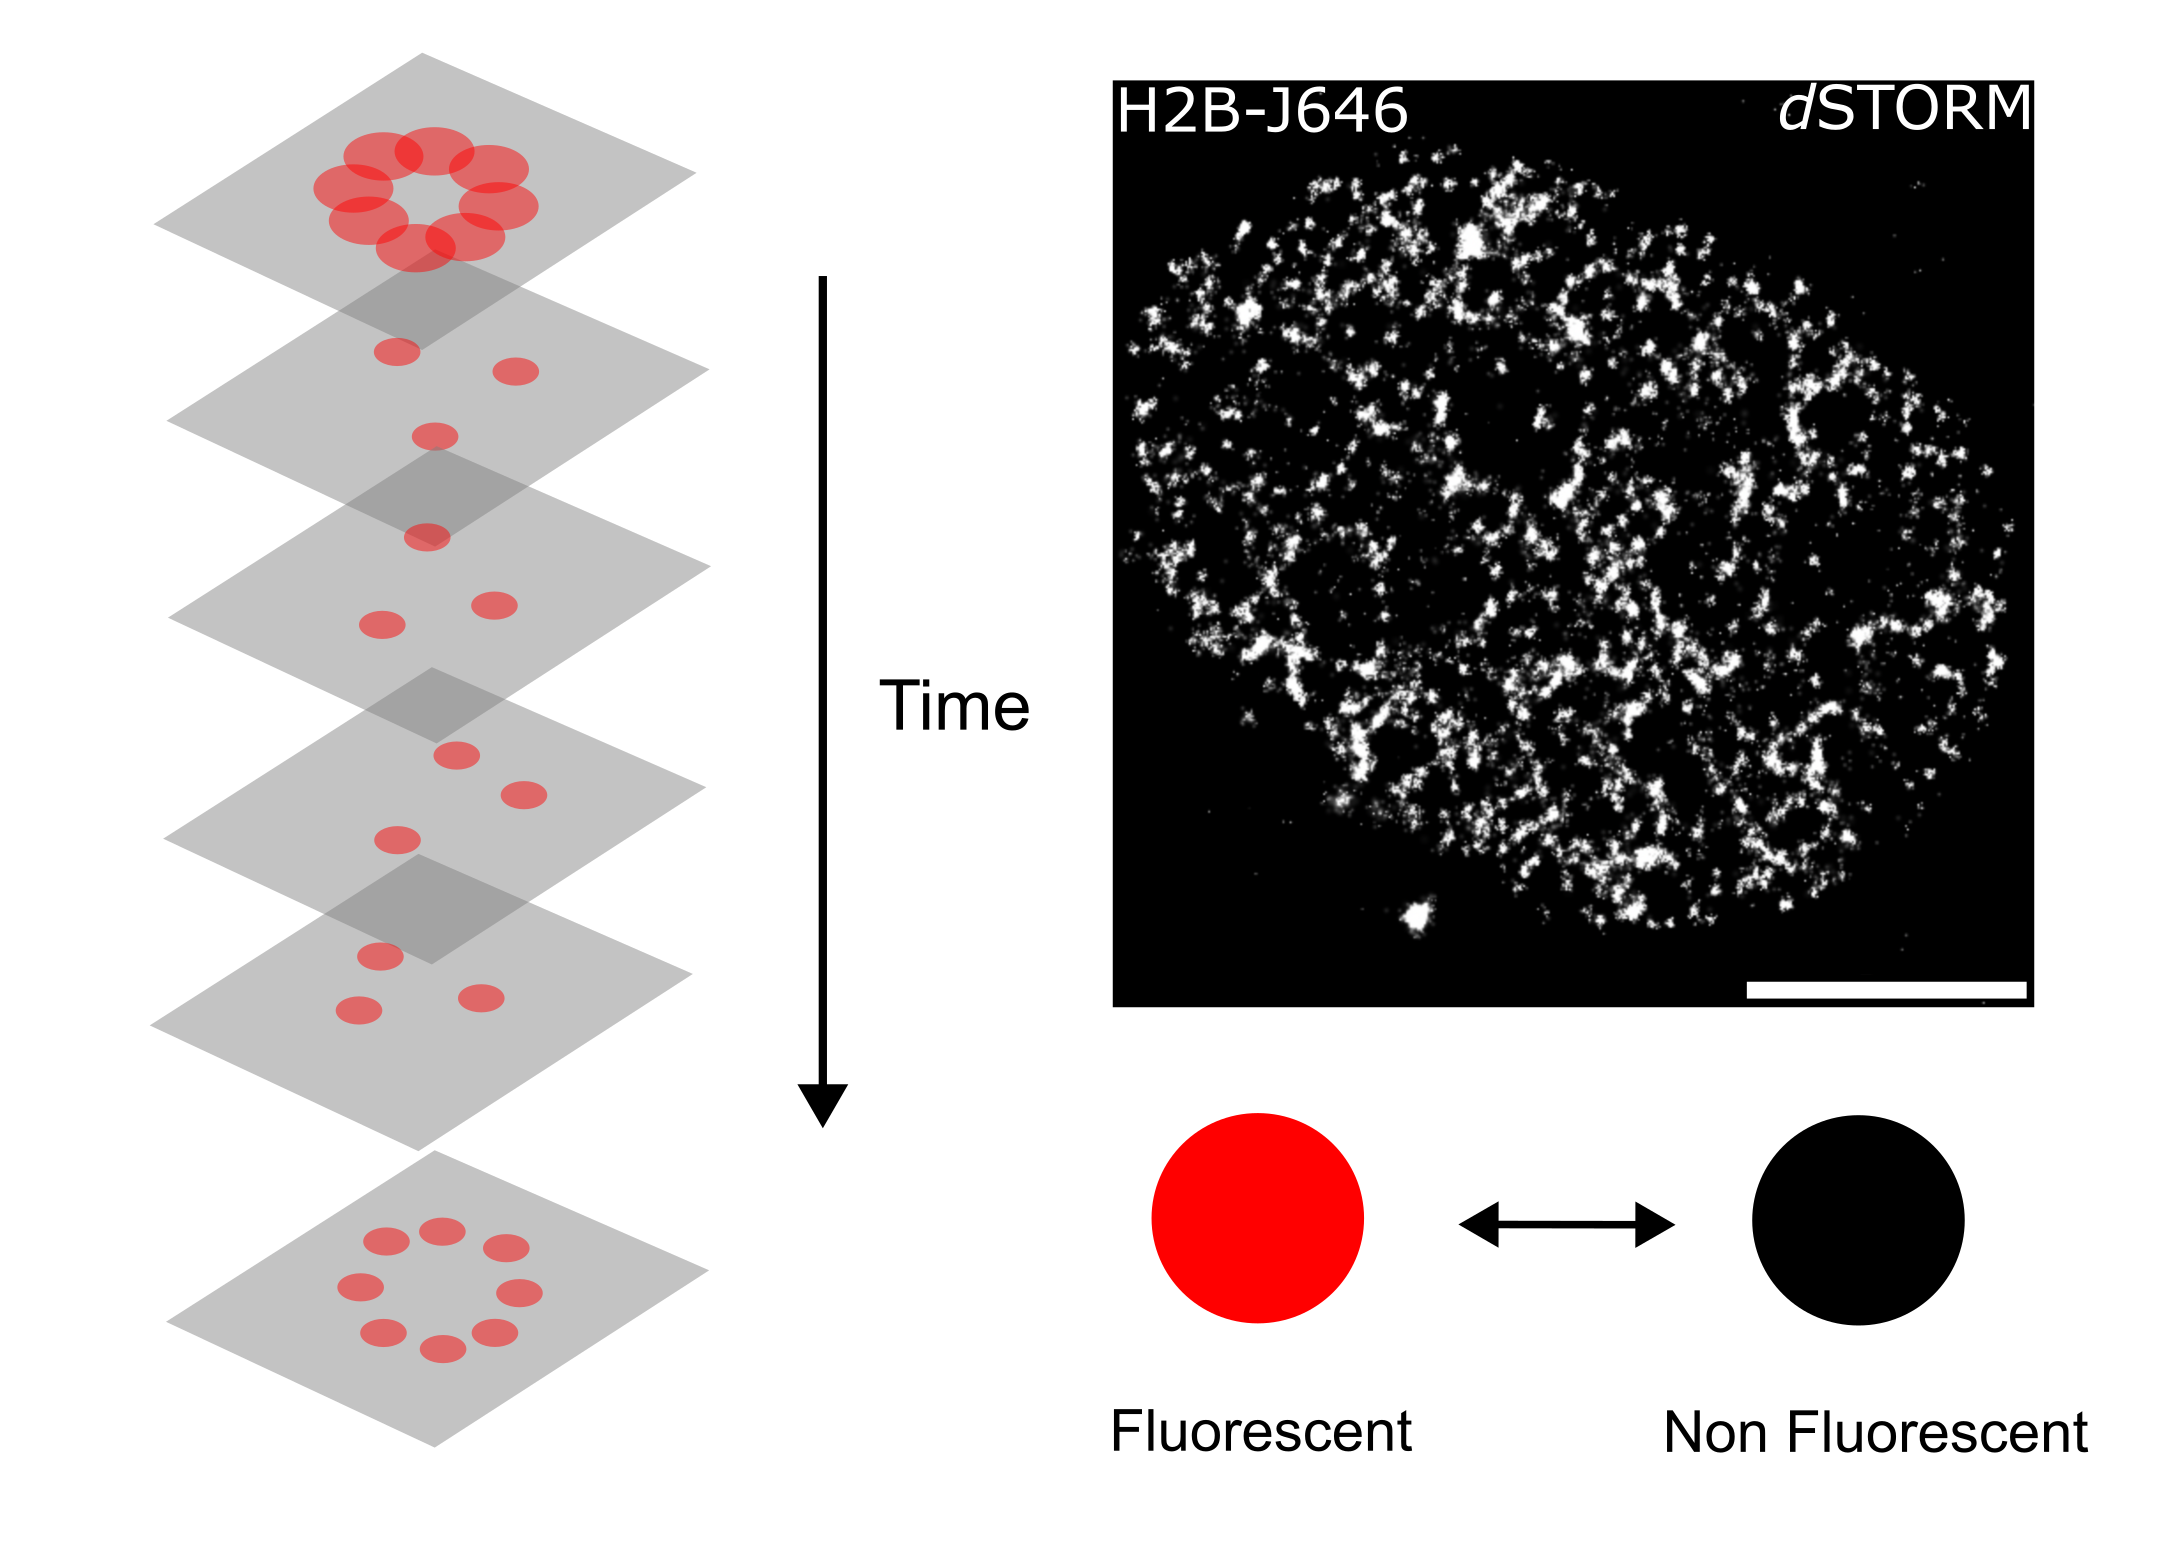
\includegraphics[width=12cm]{media/Intro.png}
\caption{\textbf{Stochastic optical reconstruction microscopy (STORM)}. (A) Single molecules are resolved by separating their fluorescent emission in time, using fluorophores with multiple photophysical states (B) Example super-resolution image of H2B protein in a living Hela cell nucleus at 37C, 5 percent CO2. Image reconstructed from $10^{3}$ 10ms frames. Scalebar 5um.}
\end{figure}

\begin{figure}[t]
\centering
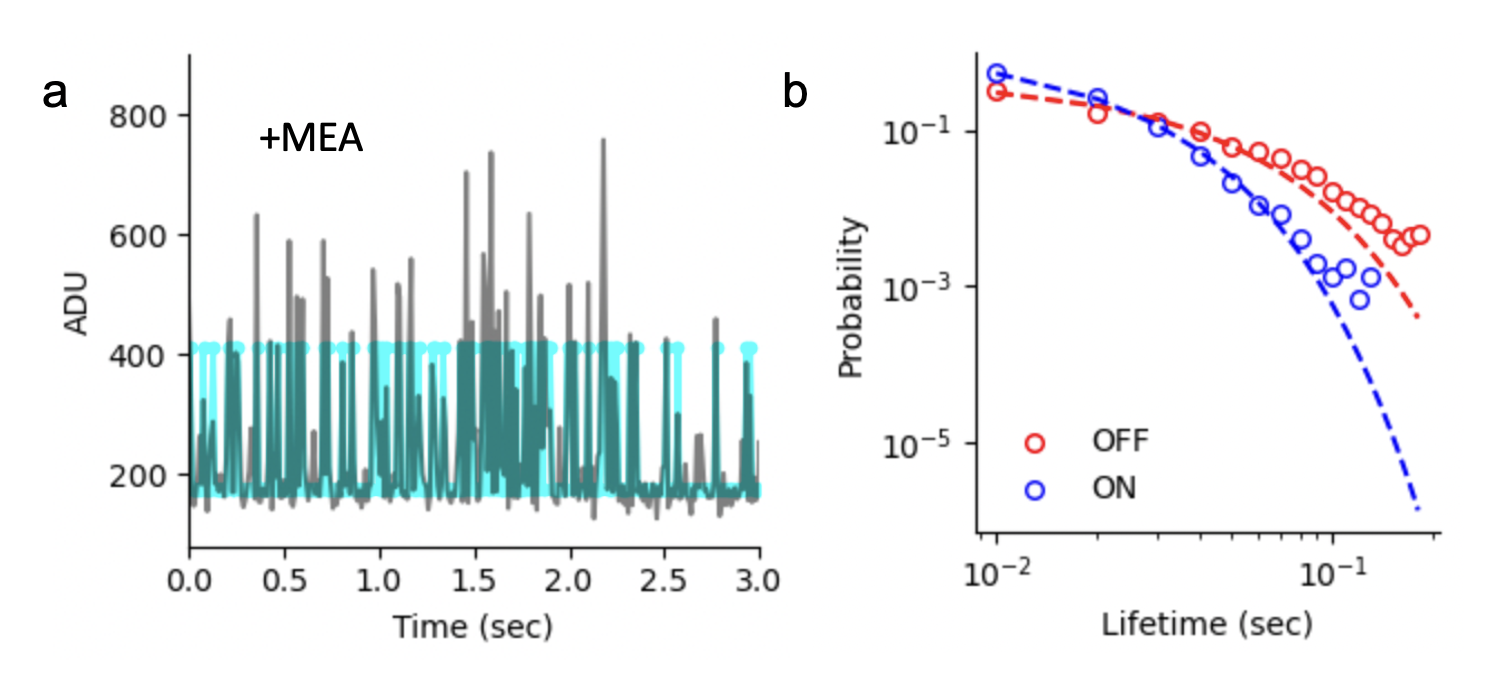
\includegraphics[width=13cm]{media/Lifetime.png}
\caption{Photoswitching of JF646 bound to H2B-HaloTag. (a) Peak intensity fluctuations of a putatively isolated JF646 molecule exicted at 640nm and imaged with 10ms exposure time in the presence of 100mM MEA buffer. Fit of a Poisson HMM is shown in cyan (b) ON and OFF state lifetime distributions found by pooling data from 16 JF646 spots in a single HeLa cell nucleus. Single component exponential fits shown as solid lines.}
\end{figure}


\section{The Image Likelihood}

It is common to describe the optical impulse response of a microscope as a two-dimensional isotropic Gaussian \parencite{Zhang2007}. This is an approximation to the more rigorous diffraction models given by \parencite{Richards1959,Gibson1989}. Over a continuous domain, the impulse response reads

\begin{equation*}
O(u,v) = \frac{1}{2\pi\sigma_{\bold{x}}^{2}}e^{-\frac{(u-\theta_{u})^{2}+(v-\theta_{v})^{2}}{2\sigma_{\bold{x}}^{2}}}
\end{equation*}

The above expression can be interpreted as a probability distribution over locations where a photon can be detected. Therefore, for discrete detectors, we discretize this expression by integrating over pixels. The number of photon arrivals will follow Poisson statistics, with expected value

\begin{equation*}
\mu_{k} = i_{0}\left(\int_{u_{k}-\delta /2}^{u_{k}+\delta /2} O(u; \theta_{u})du \right)\left(\int_{v_{k}-\delta /2}^{v_{k}+\delta /2} O(v;\theta_{v})dv \right)
\end{equation*}

The scalar quantity $i_{0}$ represents the amplitude of the signal, which is proportional the quantum efficiency of a pixel $\eta$, the duration of exposure, $\Delta$, and the number of photons emitter by a fluorescent molecule $N_{0}$. With no loss of generality, $\Delta = \eta = 1$ and there is a single free parameter $N_{0}$. Terms above in parentheses are simply integrals of Gaussian functions and can be evaluated analytically. I define them as $\Gamma_{u},\Gamma_{v}$, respectively. For example,

\begin{align*}
\Gamma_{u} &\vcentcolon  \int_{0}^{u_{k}+\delta /2 - \theta_{u}} O(u)du - \int_{0}^{u_{k}-\delta /2 - \theta_{u}} O(u)du\\
&= \frac{1}{2}\left(\mathrm{erf}\left(\frac{u_{k}+\frac{\delta}{2}-\theta_{i}}{\sqrt{2}\sigma_{\bold{x}}}\right) -\mathrm{erf}\left(\frac{u_{k}-\frac{\delta}{2}-\theta_{i}}{\sqrt{2}\sigma_{\bold{x}}}\right)\right)
\end{align*}

where we have used the common definition $\mathrm{erf}(z) = \frac{2}{\sqrt{\pi}}\int_{0}^{z}e^{-t^{2}}dt$. Recall the central objective of SMLM is to infer a set of molecular coordinates $\theta=(\theta_{u},\theta_{v})$ from measured low resolution images $\bold{x}$. In general, the likelihood on a particular pixel $p(\bold{x}_k\lvert\theta)$ is taken to be a convolution of Poisson and Gaussian distributions, due to shot noise $p(s_{k}) = \mathrm{Poisson}(\mu_{k})$ and sensor readout noise $p(\xi_{k}) = \mathcal{N}(o_{k},w_{k}^{2})$ 

\begin{figure}[t]
\begin{center}
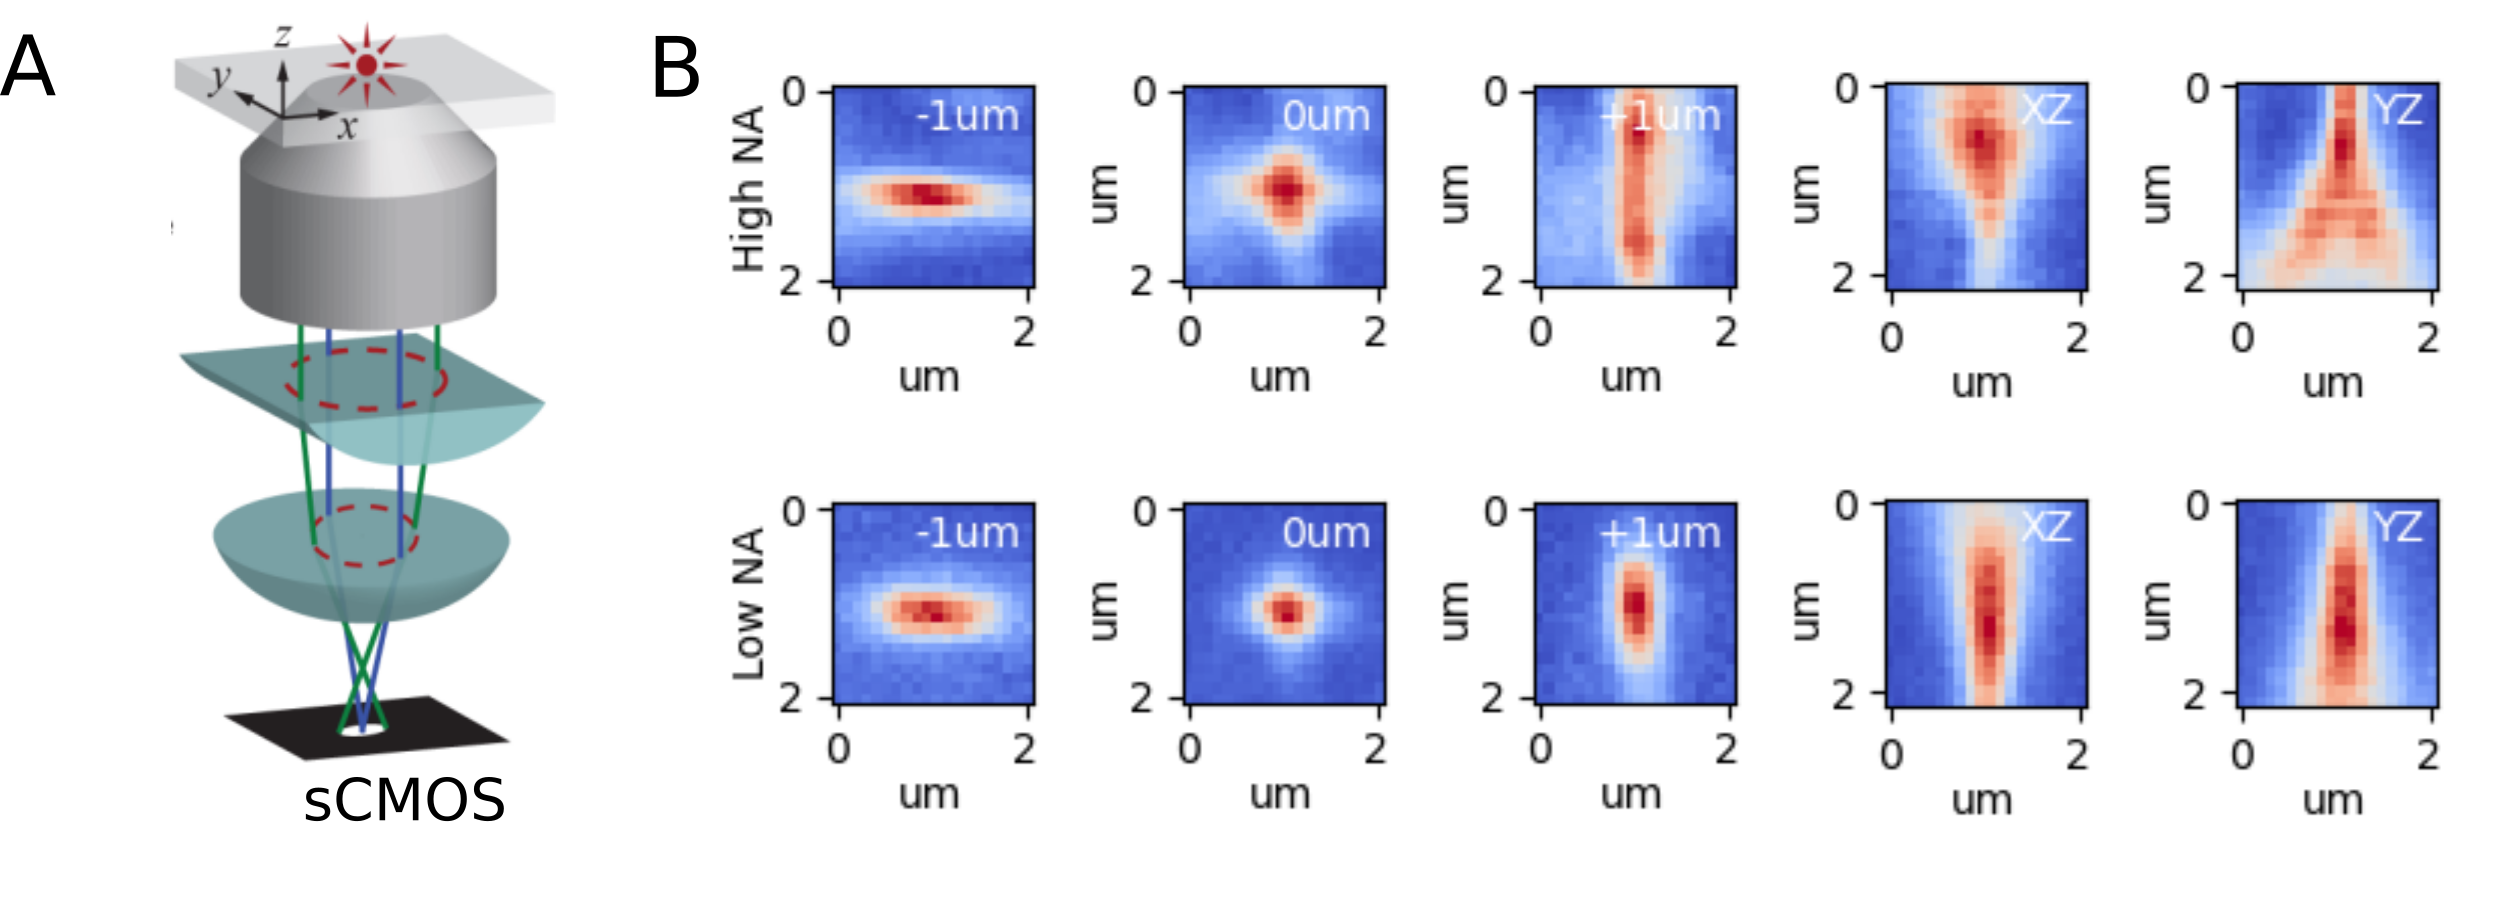
\includegraphics[width=14cm]{media/Astigmatism-Crop.png}
\end{center}
\caption{}
\end{figure}


\begin{figure}[t]
\begin{center}
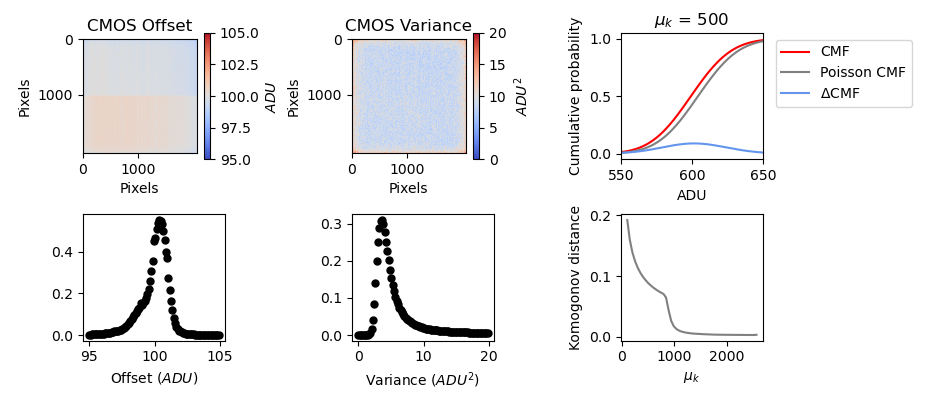
\includegraphics[width=16cm]{media/Noise.png}
\end{center}
\caption{\textbf{Noise model for CMOS cameras used for MLE}. (left)) CMOS offset for zero incident photons (middle) CMOS variance for zero incident photons (upper right) Cumulative mass function for the convolution distribution and its Poisson approximation for rate parameter $\mu_{k} = 500$ counts (lower right) Komogonov distance measured as a function of rate parameter $\mu_{k}$}
\end{figure}


\begin{equation}
p(\bold{x}_{k}\lvert\theta) = A\sum_{q=0}^{\infty} \frac{1}{q!}e^{-\mu_{k}}\mu_{k}^{q}\frac{1}{\sqrt{2\pi}w_{k}}e^{-\frac{(\bold{x}_{k}-g_{k}q-o_{k})^2}{2 w_{k}^{2}}} \approx \mathrm{Poisson}(\mu_{k}')
\end{equation}

where $A$ is some normalization constant. For the sake of generality, we include a per-pixel gain factor $g_{k}$, which is often unity. Sampling from $p(\bold{x}_{k}\lvert\theta)$ is trivial; however, for computation of a lower bound on uncertainty in $\theta$, the summation in (1) can be difficult to work with. Therefore, we choose to use a Poisson approximation for simplification, valid under a range of experimental conditions (Huang2013). After subtraction of a known offset $o_{k}$ of the pixel array, which can be easily measured, we have $\mu_{k}' = \mu_{k} + w_{k}^{2}$.

Under the Poisson approximation in the likelihood, the model negative log-likelihood is

\begin{equation}
\ell(\bold{x}\lvert\theta) = -\log \prod_{k} \frac{e^{-\left(\mu_{k}'\right)}\left(\mu_{k}'\right)^{n_{k}}}{n_{k}!} = \sum_{k}  \log n_{k}! + \mu_{k}' - n_{k}\log\left(\mu_{k}'\right)
\end{equation}

Localization then proceeds by minimization of $\ell(\bold{x}\lvert\theta)$. 


\subsection{Maximization of density, minimization of error}

The distribution of a particular biomolecule in the cell can be described as a probability density over a two-dimensional space, casting super-resolution as a density estimation problem. Intuitively, the spatial resolution of SMLM images then increases as we draw more samples from this density - a concept which is made mathematically precise by the so-called Fourier ring correlation or FRC. Using FRC, one can compute image resolution as the spatial frequency at which a correlation function in the frequency domain drops below a threshold, typically taken to be $1/7$ (See Supplement). According to this theory, reducing localization uncertainty while increasing the number of samples, results in an increase in image resolution (Nieuwenhuizen 2013). However, there remains a fundamental limit to the the minimal localization uncertainty which can be obtained.


\begin{equation*}
\mathrm{FRC}(q) = \frac{\sum_{\vec{q}\in\mathrm{circle}}\tilde{f_{1}}(\vec{q})\tilde{f_{2}}(\vec{q})^{*}}{\sqrt{\sum_{\vec{q}\in\mathrm{circle}}\lvert f_{1}(\vec{q})\lvert^{2}}\sqrt{\sum_{\vec{q}\in\mathrm{circle}}\lvert f_{2}}(\vec{q})\lvert^{2}}
\end{equation*}


\begin{figure}[t]
\begin{center}
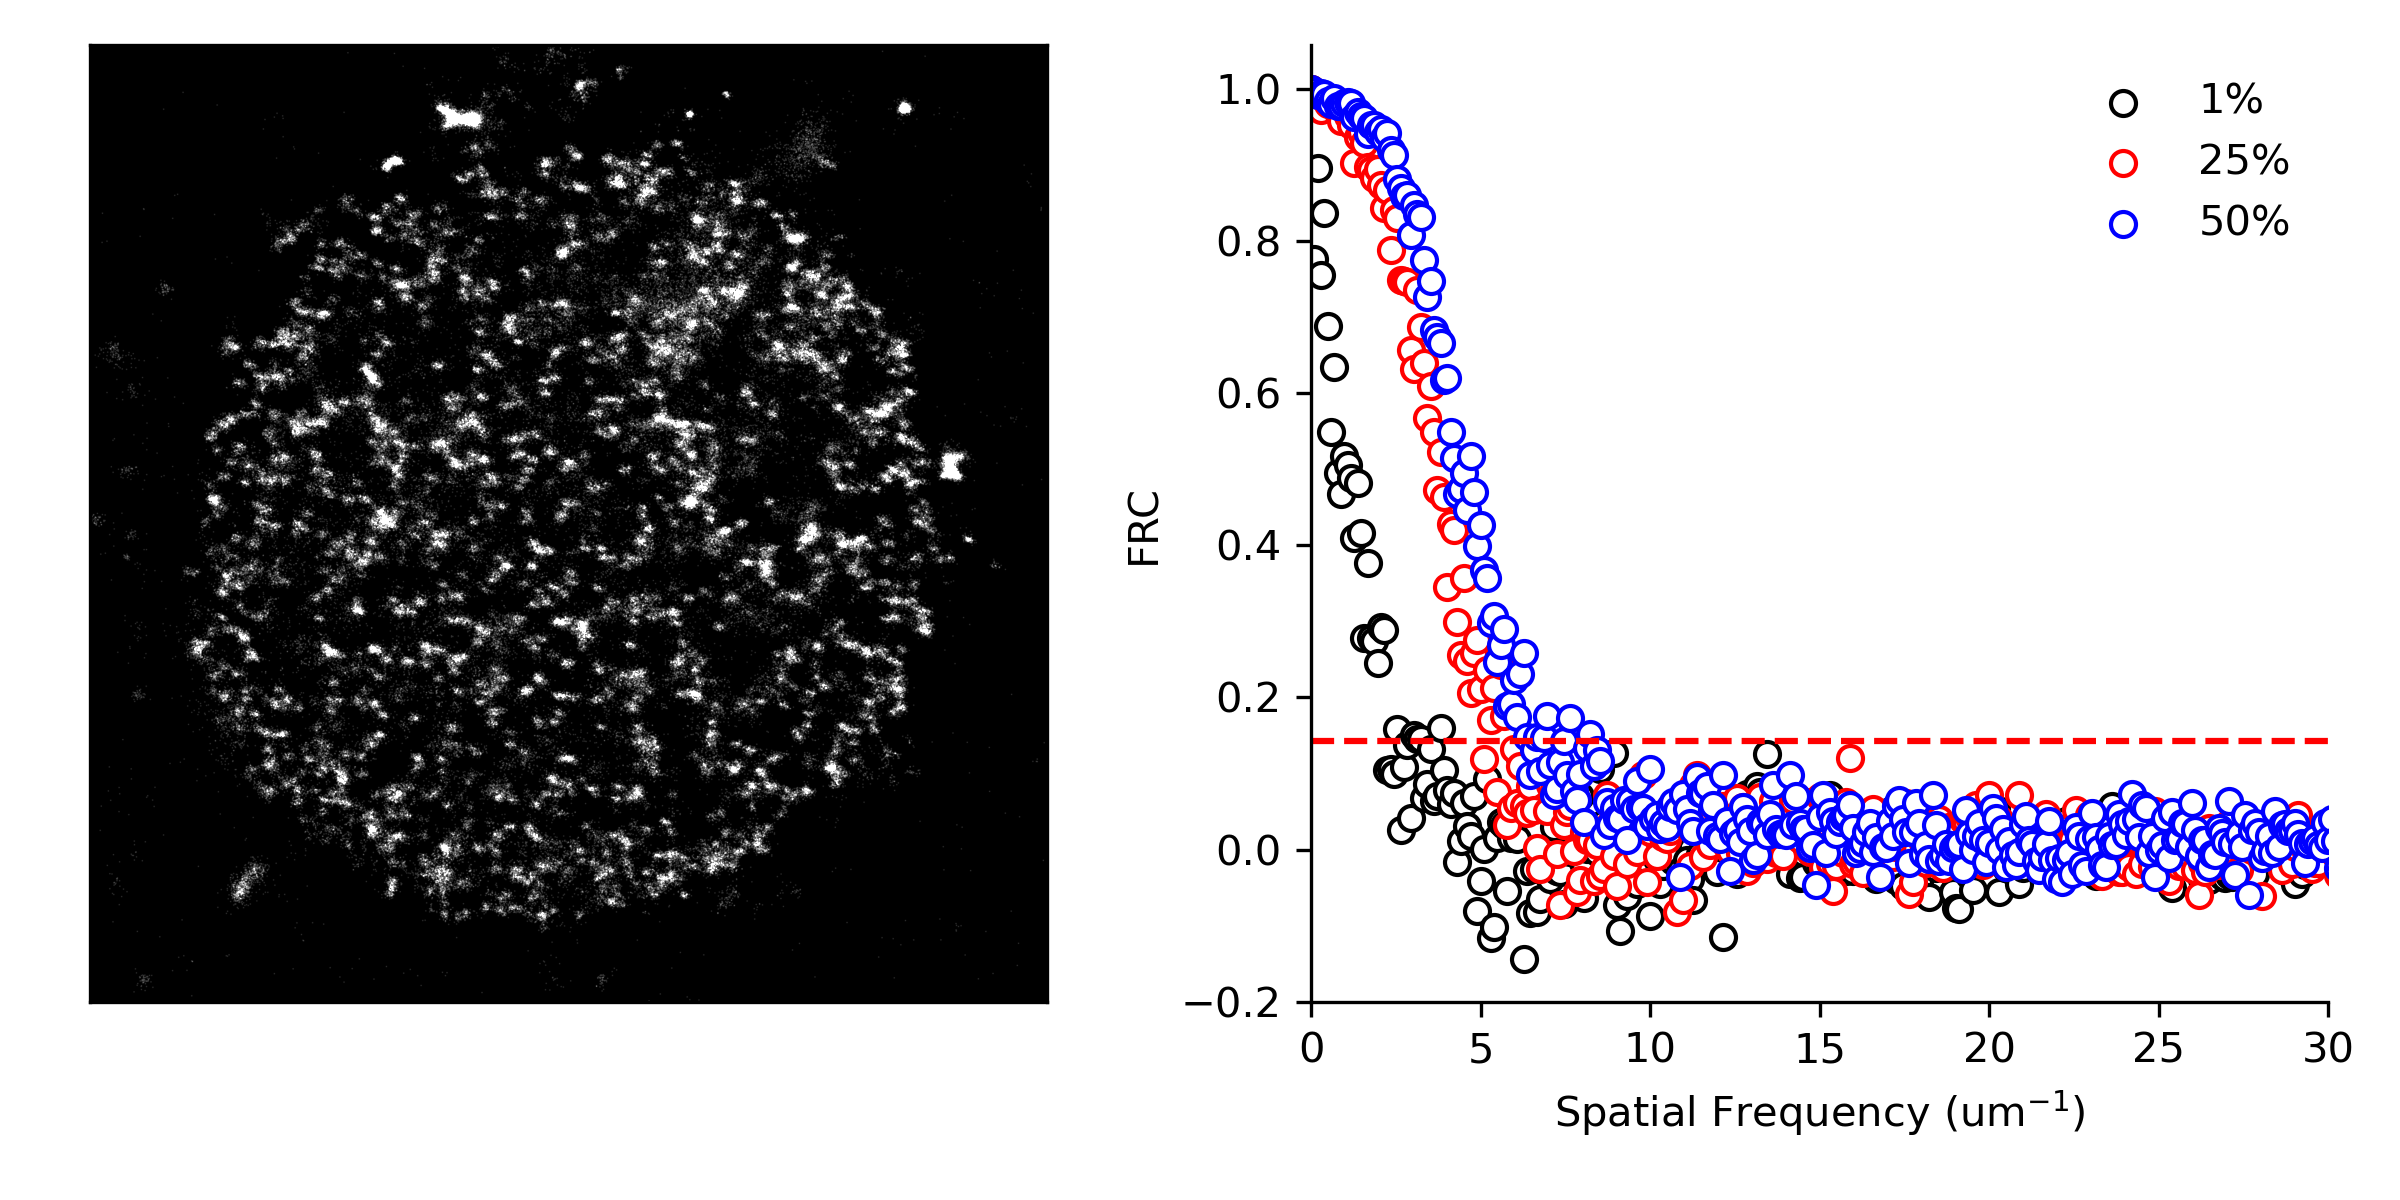
\includegraphics[width=14cm]{media/FRC.png}
\end{center}
\caption{\textbf{Noise model for CMOS cameras used for MLE}. (left)) CMOS offset for zero incident photons (middle) CMOS variance for zero incident photons (upper right) Cumulative mass function for the convolution distribution and its Poisson approximation for rate parameter $\mu_{k} = 500$ counts (lower right) Komogonov distance measured as a function of rate parameter $\mu_{k}$}
\end{figure}


Localization uncertainty, typically the RMSE of a maximum likelihood or similar statistical estimator, is bounded from below by the inverse of the Fisher information matrix, known as the Cramer-Rao lower bound (Chao 2016). Localization uncertainties in sparse conditions are often tens of nanometers, although recent work on integration of Bayesian priors with modulation enhanced SMLM (meSMLM) or structured illumination with MINFLUX, has reduced spatial resolution below to a few nanometers (Kalisvaart 2022, Gwosh 2020). Nevertheless, managing the increase in localization uncertainty at high labeling density remains a major bottleneck to SMLM. Static uncertainty due to molecular crowding can be partially amelioriated by using pairwise or higher-order temporal correlations within a pixel neighborhood, known as stochastic optical fluctuation imaging or SOFI (Dertinger 2009). Other approaches such as stimulated emission and depletion (STED) imaging bring control over the photophysical state of a chosen subset of the sample, yet the need for laser scanning prevents widespread application in live-cell studies. The spatial resolution and relative simplicity of SMLM techniques remains unmatched, inciting an effort to increase the resolution of SMLM techniques and explore avenues towards time resolved SMLM.



\ProvidesFile{ch3.tex}[Chapter3]
\chapter{QUANTUM ENHANCED LOCALIZATION MICROSCOPY WITH A SINGLE PHOTON AVALANCHE DIODE ARRAY}
\ix{physics//Physics appendix}

\section{Background}

\subsection{A brief introduction to quantum optics}

Experimental techniques have surfaced which take advantage of the quantum nature of light to enhance imaging methods. The advent of fast and sensitive detectors allows us to measure electromagnetic fields at a timescale where quantum effects can be seen. We often speak of methods such as photon counting or photon statistics, and it is prudent to briefly define the photon and how it can be measured with this technology.

Quantization of the electromagnetic field generally begins by writing a Fourier expansion of solutions to Maxwell's equations called \emph{modes} and identifying the canonical position and momentum variables. This procedure is out of the scope of this thesis. Instead, we start by stating the major result of quantization, in which each mode of the field is quantized as a quantum harmonic oscillator. As such, the Hamiltonian for one particular mode has energy eigenvalues $E_{k} = \hbar\omega_{k}(n + \frac{1}{2})$ for mode $k$ with frequency $\omega_{k}$. Since there may be infinitely many modes, the wavefunction is $\ket{\psi} = \ket{n_{1},n_{2},...}$ where $n_1$ is the number of photons in the first mode, $n_2$ is the number of photons in the second mode, and so on. The number operator for the $k$-th mode gives $\hat{n}_k\ket{\psi} = n_{k}\ket{\psi}$.

The number operator $\hat{n}_k = \hat{a}_k^\dagger\hat{a}_k$ is defined in terms of operators $\hat{a}_k$ and $\hat{a}_k^\dagger$ which are photon annihilation and creation operators for the $k$-th mode, respectively. These operators satisfy the commutation relations $[\hat{a}_k, \hat{a}_{k'}^\dagger] = \delta_{kk'}$ and $[\hat{a}_k, \hat{a}_{k'}] = [\hat{a}_k^\dagger, \hat{a}_k^\dagger] = 0$. The action of the annihilation and creation operators on the joint number states is:

\begin{equation*}
\hat{a}_k \ket{n_1, n_2, ...} = n_k \ket{n_1, n_2, ...} \;\;
\hat{a}_k^\dagger \ket{n_1, n_2, ...} = (n_k +1) \ket{n_1, n_2, ...}
\end{equation*}

\subsection{Photon statistics}

\begin{figure*}[t]
\centering
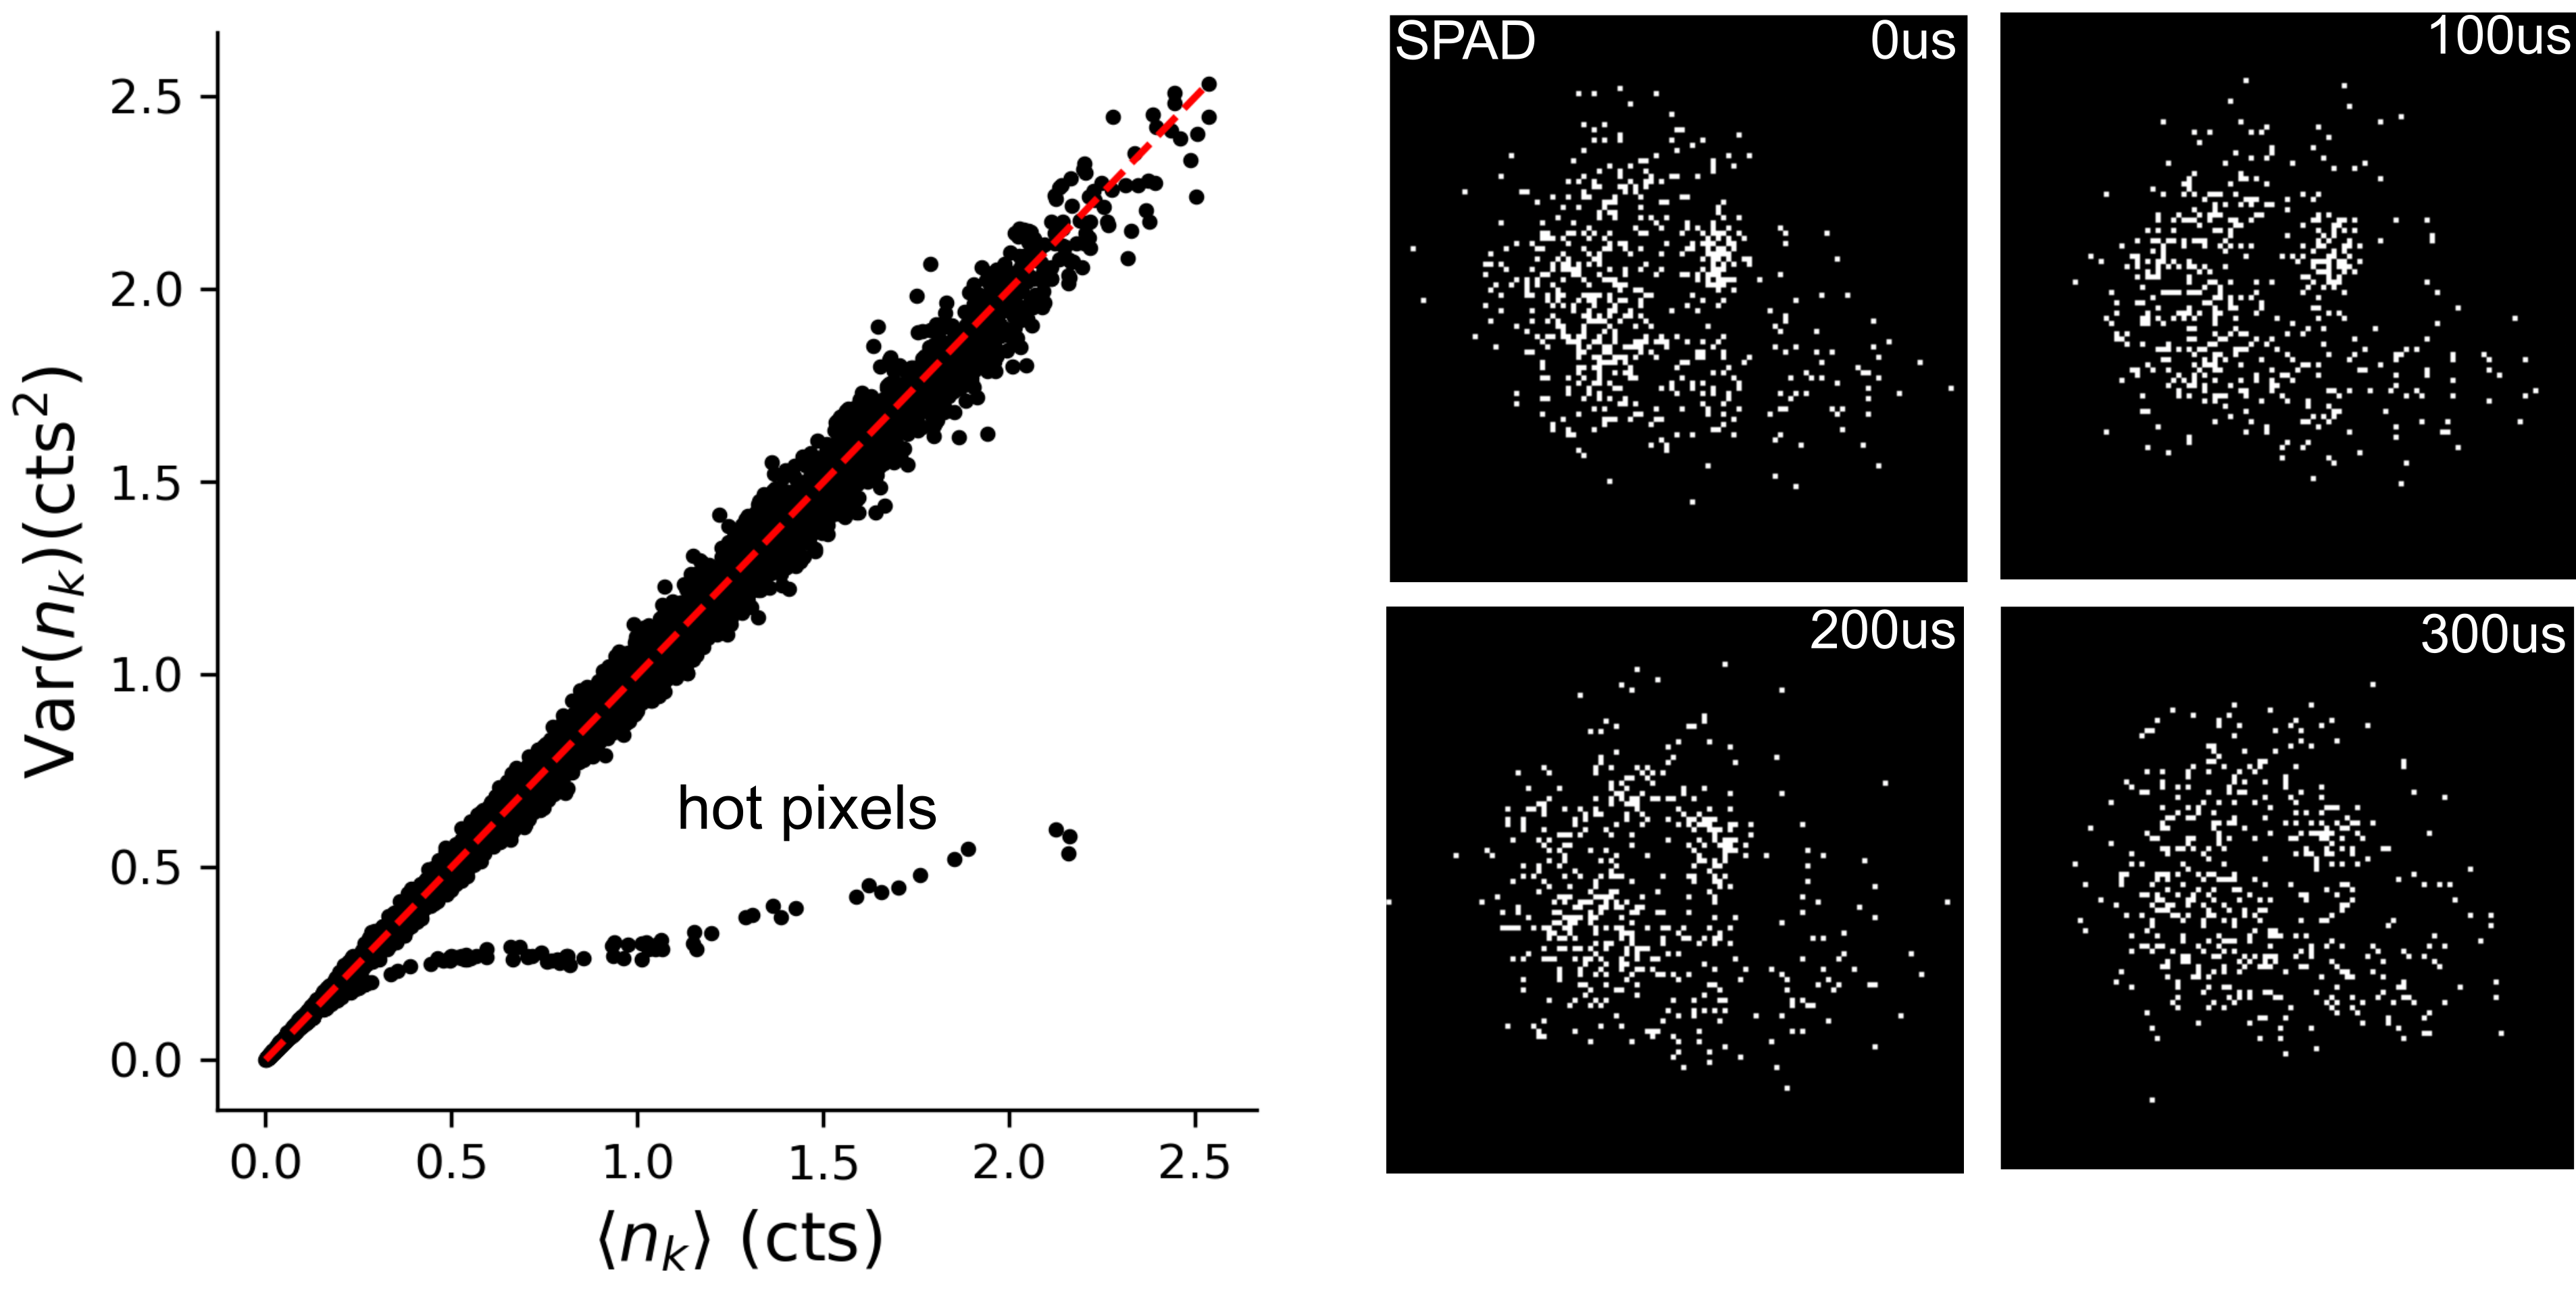
\includegraphics[width=16cm]{/Users/cwseitz/git/cwseitz.github.io/docs/phd/spad/spad/media/Laser-Stats.png}
\caption{\textbf{Poissonian photon statistics of a Gaussian laser spot}. (left) Fano factor plot of pixel-wise variance in photon counts with respect the average photon counts, for 100$\mu$s exposures of a Gaussian beam pulsed at 10MHz. Equal mean and variance (Poisson statistics) showed as a dashed red line. (right) Example images taken in sequence with the SPAD array.}
\label{fig:fig29}
\end{figure*}    

There are certain states $\ket{\psi}$ which have special properties, such as the coherent state. Coherent states resemble classical oscillations of the EM field. A coherent state $\ket{\alpha}$ is defined as the eigenstate of the annihilation operator $\hat{a}$:

\begin{equation*}
\hat{a} \ket{\alpha} = \alpha \ket{\alpha}
\end{equation*}

where $\alpha$ is a complex number. The coherent state for a single mode field is given by:

\begin{equation*}
\ket{\alpha} = e^{-\frac{\lvert\alpha\lvert^2}{2}} \sum_{n=0}^\infty \frac{\alpha^n}{n!} \ket{n}
\end{equation*}

It turns out that if we measure a number of photons in this state, we would find that the number of photons has Poisson statistics. To see this, we calculate the probability $p(n)$ of finding $n$ photons in a coherent state $\ket{\alpha}$:

\begin{equation*}
p(n) = \lvert \bra{n} \ket{\alpha} \lvert^2 = \lvert e^{-\frac{\lvert\alpha\lvert^2}{2}} \frac{\alpha^n}{n!} \lvert^2 = e^{-\lvert\alpha\lvert^2} \frac{\lvert\alpha\lvert^{2n}}{n!}
\end{equation*}

This is simply the Poisson distribution with mean $\langle \hat{n} \rangle = \lvert\alpha\lvert^2$. The variance of the photon number distribution in a coherent state is also $\lvert\alpha\lvert^2$, characteristic of Poisson statistics, where the mean and variance are equal. Poissonian fluctuations of a Gaussian beam can be spatially resolved using a single photon avalanche diode (SPAD) array (Figure \ref{fig:fig29}).

In contrast, single photon states, such as $\ket{1}$, do not necessarily follow Poisson statistics. This state could be prepared by an isolated single photon source such as a fluorescent dye molecule, quantum dot, or nitrogen vacancy, which can produce only a single photon at at time. This phenomenon is referred to as \emph{fluorescence antibunching} where photons tend to be detected as isolated events rather than in bursts or bunches. Single photon sources have a fluorescence lifetime, typically on the order of nanoseconds, which results in a sequence of photon arrivals with a more regular structure than would be expected under Poisson statistics. Note that for such a single photon source the single-mode field can be in state $\ket{1}$ but not state $\ket{2}$ at any given time. If more single photon sources are present or multi-level relaxations occur, states beyond $\ket{1}$ are possible. This has led to the introduction of binomial states of the quantized field \parencite{Stoler1985}. This fact is leveraged in the following sections, to count the number of single photon sources in a region of interest using a SPAD array.

\section{Second-order coherence}

The second-order coherence function, $ g^{(2)}(\tau) $, is a fundamental tool in quantum optics, providing insight into photon statistics. It can be expressed in terms of photon counts $ n(t) $ as:

\begin{equation}
g^{(2)}(\tau) = \frac{\langle n(t) n(t+\tau) \rangle}{\langle n(t) \rangle^2}
\end{equation}

This formulation highlights how the intensity correlations between photons detected at times $ t $ and $ t+\tau $ are normalized by the square of the mean photon count rate, providing a dimensionless measure of the correlation. The value of $ g^{(2)}(\tau) $ and its dependence on $ \tau $ reveal essential characteristics of the light source. For sub-Poissonian statistics, which is synonymous with photon antibunching, $ g^{(2)}(0) < 1$ and the likelihood of detecting two photons in quick succession is reduced. This behavior is closely related to the fluorescence lifetime of the emitters; after emitting a photon, a fluorophore requires a characteristic time to re-enter the excited state, leading to a dip in $ g^{(2)}(\tau) $ at short $ \tau $. Coherent light, discussed in the previous section, shows no correlation between photon arrival times, resulting in $ g^{(2)}(\tau) = 1 $ for all $ \tau $. Super-Poissonian statistics, seen in thermal light, exhibit photon bunching, where $ g^{(2)}(\tau) $ starts high at $ \tau = 0 $ and decays to 1 as $ \tau $ increases, indicating a higher probability of photons arriving close together in time.

Techniques such as Hanbury Brown and Twiss (HBT) interferometry are commonly employed to measure $ g^{(2)}(\tau) $, using two single photon sensitive detectors and a beam splitter. In the following sections, we will incorporate an empirical estimate of $g^{(2)}(\tau)$ into a framework for inference of the number of fluorescent emitters in a diffraction limited region. 

\section{Quantum-enhanced localization microscopy}

Single photon avalanche diodes (SPADs) have long been the detector of choice for highly sensitive biological imaging and sensing, such as single molecule imaging and single molecule spectroscopy. Its fast temporal response and low background noise allow for the registration of a single photon with a temporal resolution as precise as several picoseconds \parencite{Bruschini2019}. However, standard SPAD detectors lack spatial resolution and are typically integrated in laser scanning microscopes for biological imaging, which significantly limits the imaging speed. Recently developed SPAD arrays removed this limitation and extended the high spatiotemporal imaging to widefield microscopy. SPAD arrays can achieve orders of magnitude higher temporal resolutions than standard cameras while preserving the SPAD detector‘s original signatures, such as single photon sensitivity, low dark count rates, and time-gated photon collection. Furthermore, the reduced readout noise and large fill-factor of recently commercialized SPAD arrays suggests their use for precision widefield bioimaging for single molecule studies. Such technologies have also attracted considerable attention in the bioimaging community for various applications including widefield fluorescence lifetime imaging \parencite{Nedbal2024,Ulku2019,Zickus2020}.

The spatial configuration of the SPAD array can also function as a two-dimensional and on-chip Hanbury-Brown and Twiss setup that measures the antibunching effect, which is a purely quantum optical phenomenon \parencite{Tenne2019,Treussart2001,Schwartz2012,Ta2010} that reports the single photon emission signature of a quantum emitter. A simplified SPAD array has been previously discussed for localization microscopy in non-sparse scenes \parencite{Israel2017} to image quantum dots beyond the diffraction limit. However, this imaging modality was challenged by a general issue encountered in fluorescent labeling, i.e., how to quantify multiple fluorophores in a diffraction-limited spot? 

The antibunching property is manifest in both the second-order coherence of photon arrivals as well as the photon counting histogram (PCH) \parencite{Chen1999,Huang2004} i.e., the distribution of the number of photons collected from a diffraction-limited volume. Importantly, the number of photons detected during high-speed imaging provides evidence for the number of single photon sources present in the imaged region. Previous studies have used the PCH to quantify the number of active fluorescent emitters by using conventional SPAD detectors in confocal setups. However, using a SPAD array, the PCH can be measured over a large field of view with spatial resolution by fast acquisition of binary images synchronized with pulsed laser excitation. 

Here, we demonstrate that the PCH can be parameterized by the number of active fluorescent emitters in a region of interest (ROI) and their associated molecular brightness. Then, by integrating the PCH into a Bayesian inference scheme, the relative probability of various numbers of fluorescent emitters can be compared, while expressing uncertainty in the molecular brightness. We experimentally demonstrate the model by counting quantum dots and varying numbers of fluorescent dye molecules attached to DNA origamis. In parallel, we theoretically examine second-order coherence of single-molecule fluorescence as a validation metric in both background-free environments and in the presence of a coherent background signal. Our findings indicate that sensitivity of the second order coherence to background conditions limits its effectiveness to scenarios with high signal-to-background ratios.

%Far-field optical microscopy is fundamentally limited by diffraction, with the maximum attainable resolution being limited to approximately half the wavelength of light. Several schemes to beat the diffraction limit have been developed in recent years. Many of these schemes utilize the concept of precise localization of isolated fluorescent emitters which blink over a time series of frames \parencite{Rust2006,Betzig2006}. An inherent problem with such methods is the requirement that fluorescent emitters be isolated, slowing down the acquisition of super-resolved images. To begin to address this issue, we leverage the fact that many fluorophores are intrinsically single photon sources and exhibit fluorescence antibunching. This property can constrain the number of active fluorescent emitters in a region of interest (ROI) and can potentially enable localization in non-sparse scenes \parencite{Ta2010,Israel2017}. 

%\begin{figure*}[t]
%\centering
%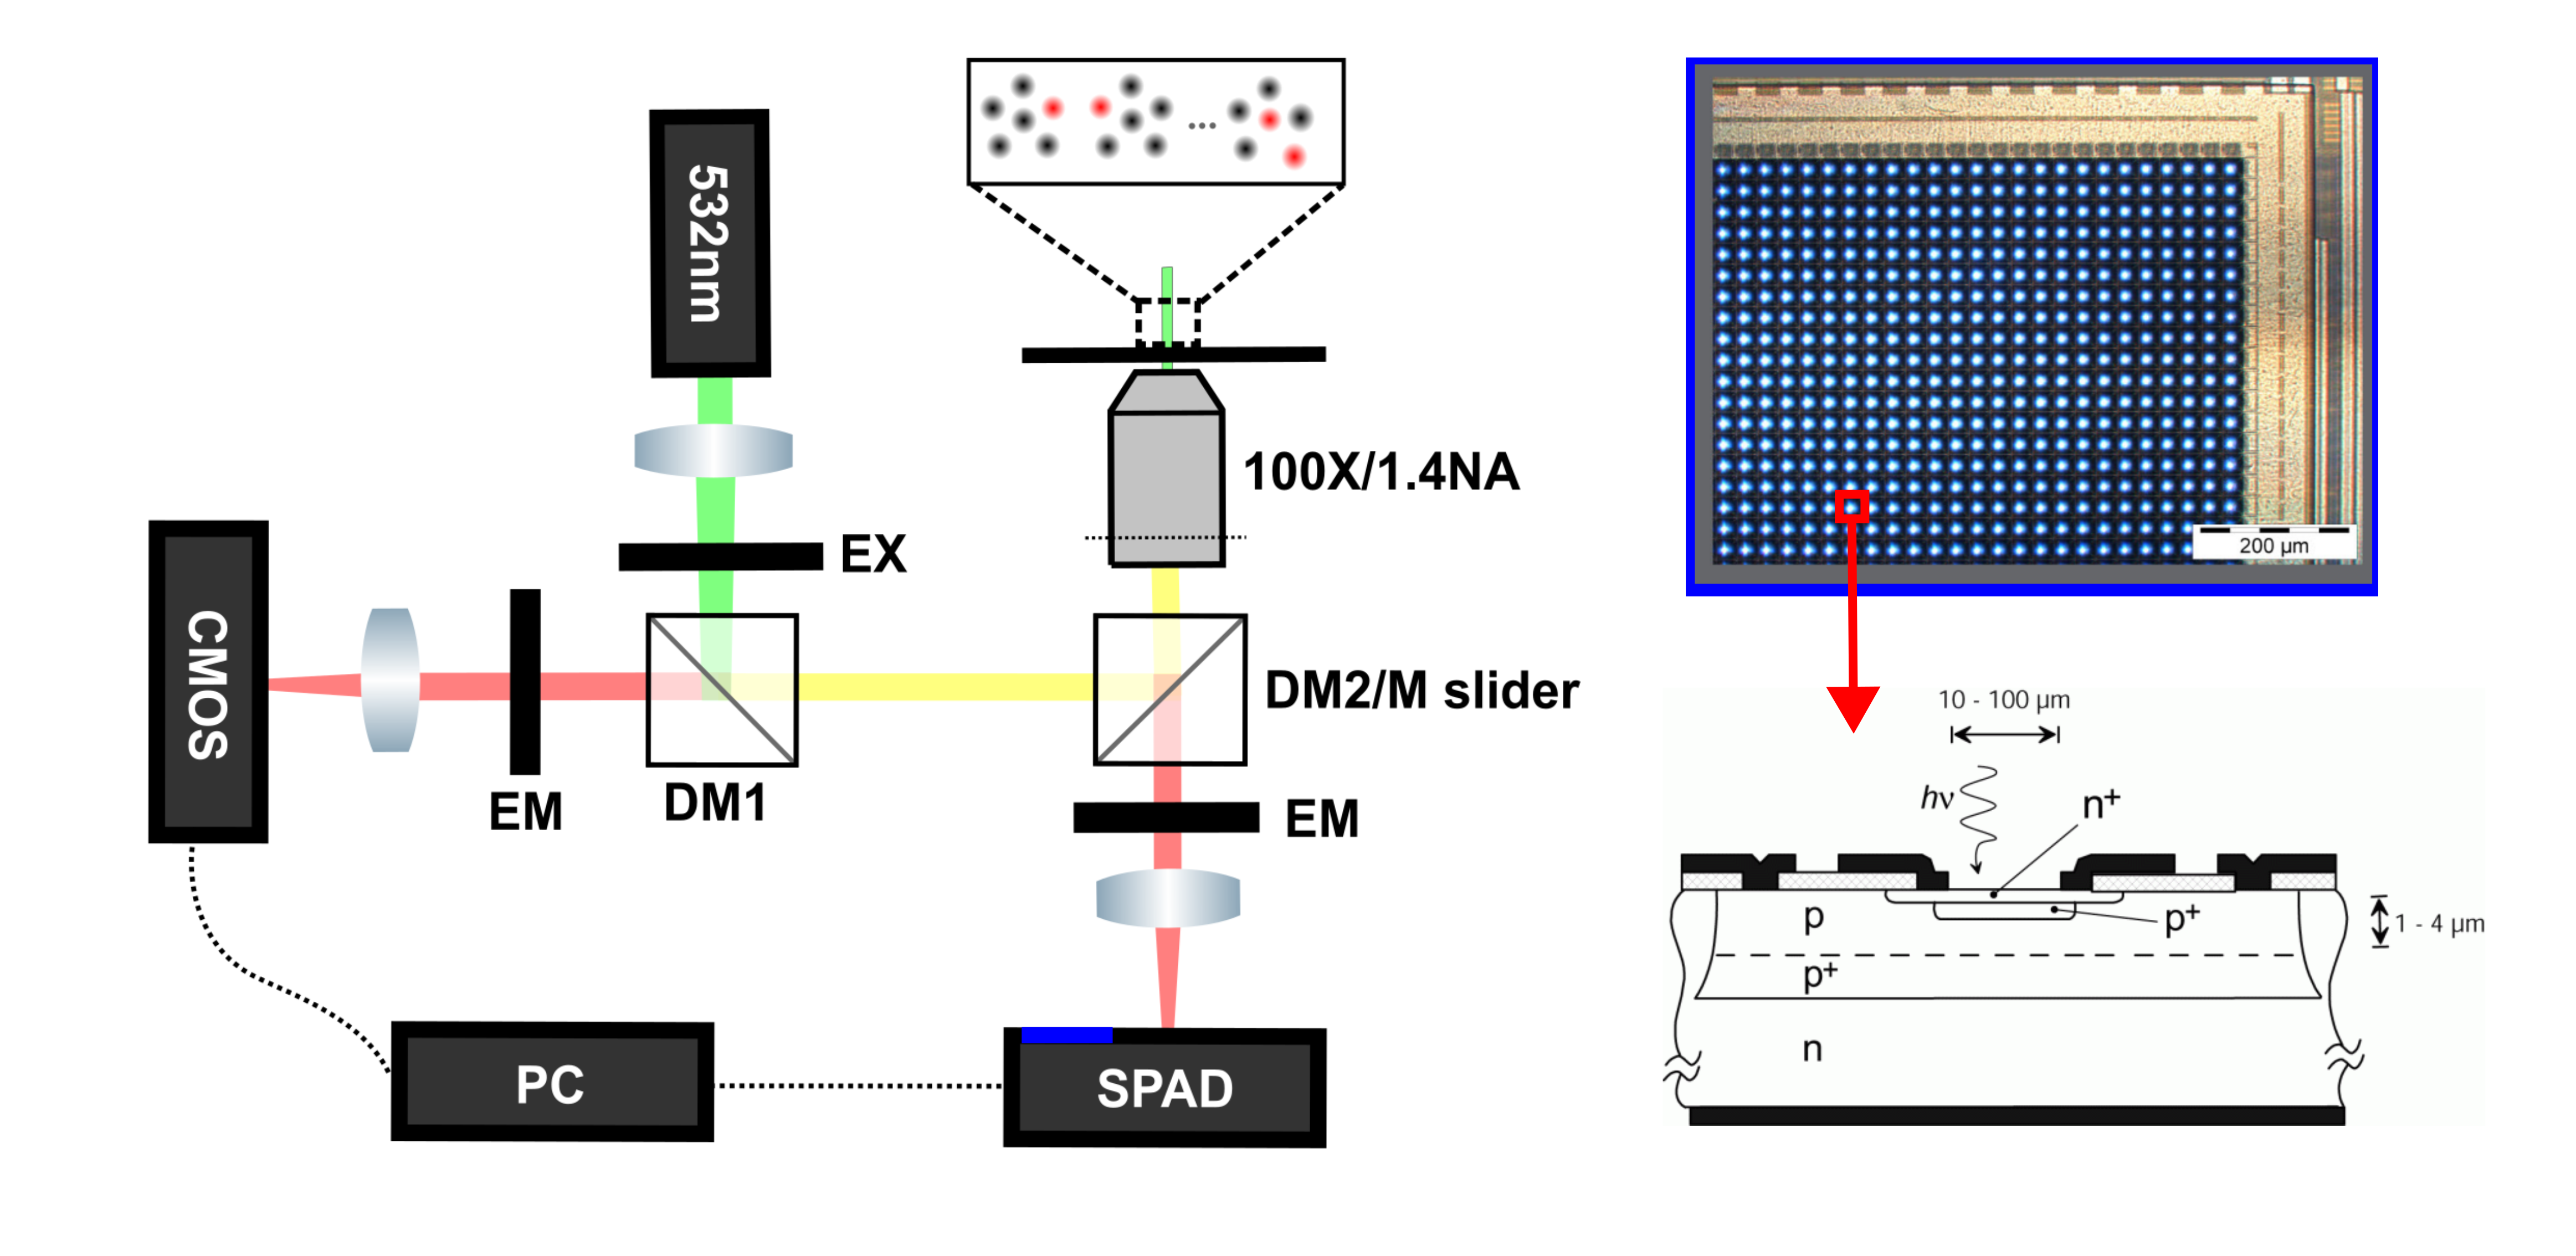
\includegraphics[width=15cm]{/Users/cwseitz/git/cwseitz.github.io/docs/phd/spad/spad/media/SPADD.png}
%\caption{\textbf{Experimental setup for widefield photon counting}. (left) A 532nm pulsed laser is directed through filtering and focusing optics to a 100X oil-immersion objective. Emisson light is collected by a CMOS or SPAD sensor. (right) Diagram of the diode at each pixel of the SPAD array. Sensor micrograph courtesy of Pi Imaging Technologies}
%\label{fig:fig00}
%\end{figure*}    

%\begin{figure*}[t]
%\centering
%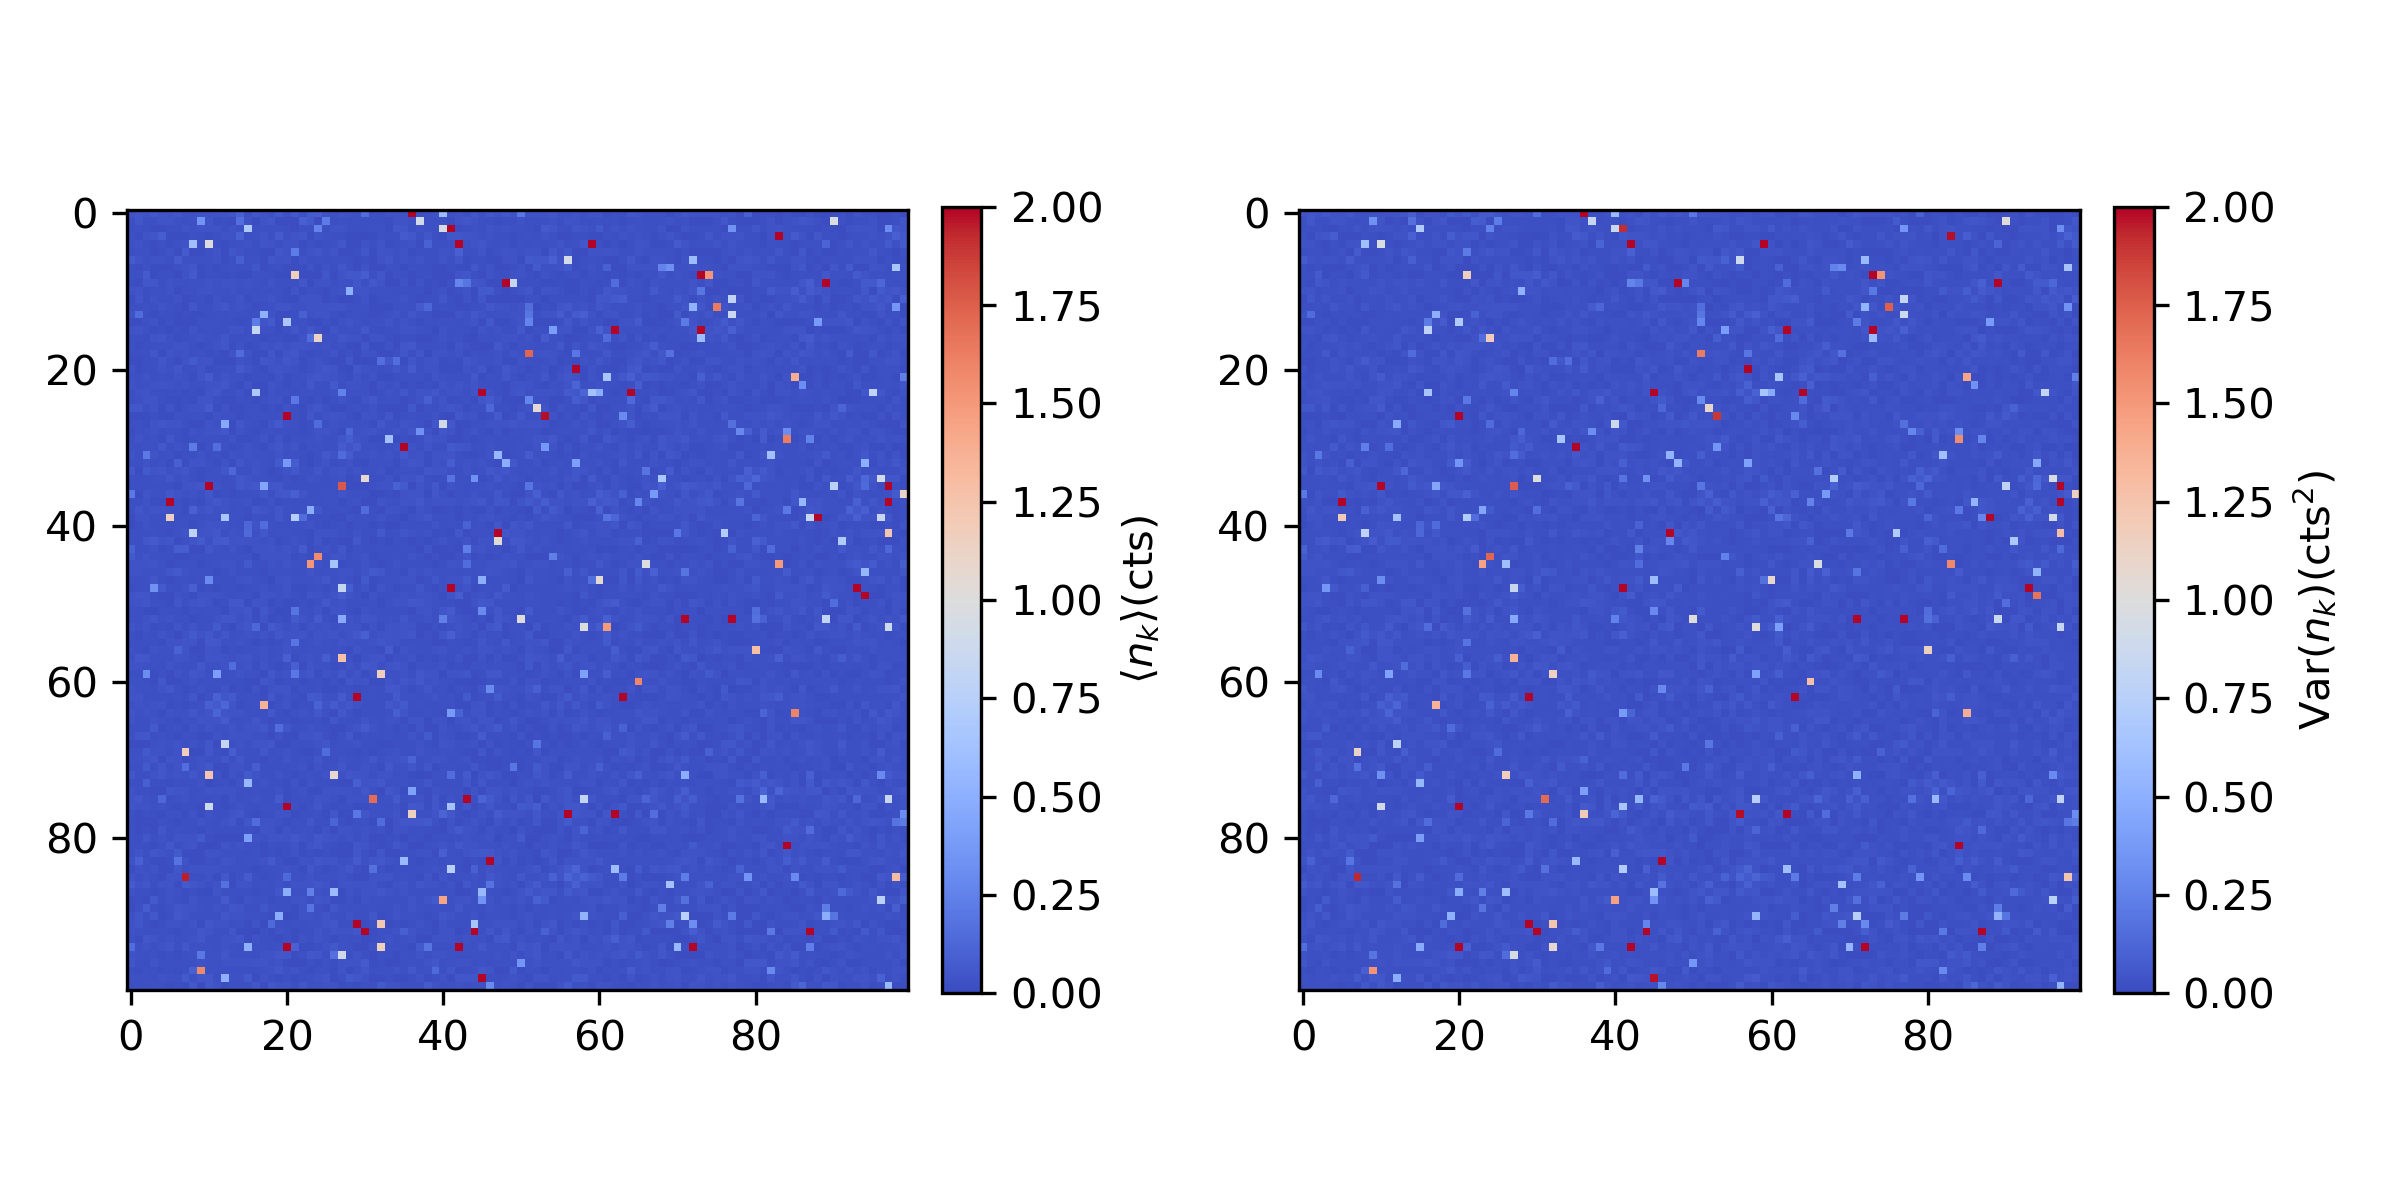
\includegraphics[width=14cm]{/Users/cwseitz/git/cwseitz.github.io/docs/phd/spad/spad/media/Dark.png}
%\caption{\textbf{Dark counts of the SPAD array}. (left) Average pixel-wise dark counts for a 100x100 pixel region exposed for 100ms (right) Variance of dark counts for 100ms exposure.}
%\label{fig:fig30}
%\end{figure*}


\begin{figure*}[t]
\centering
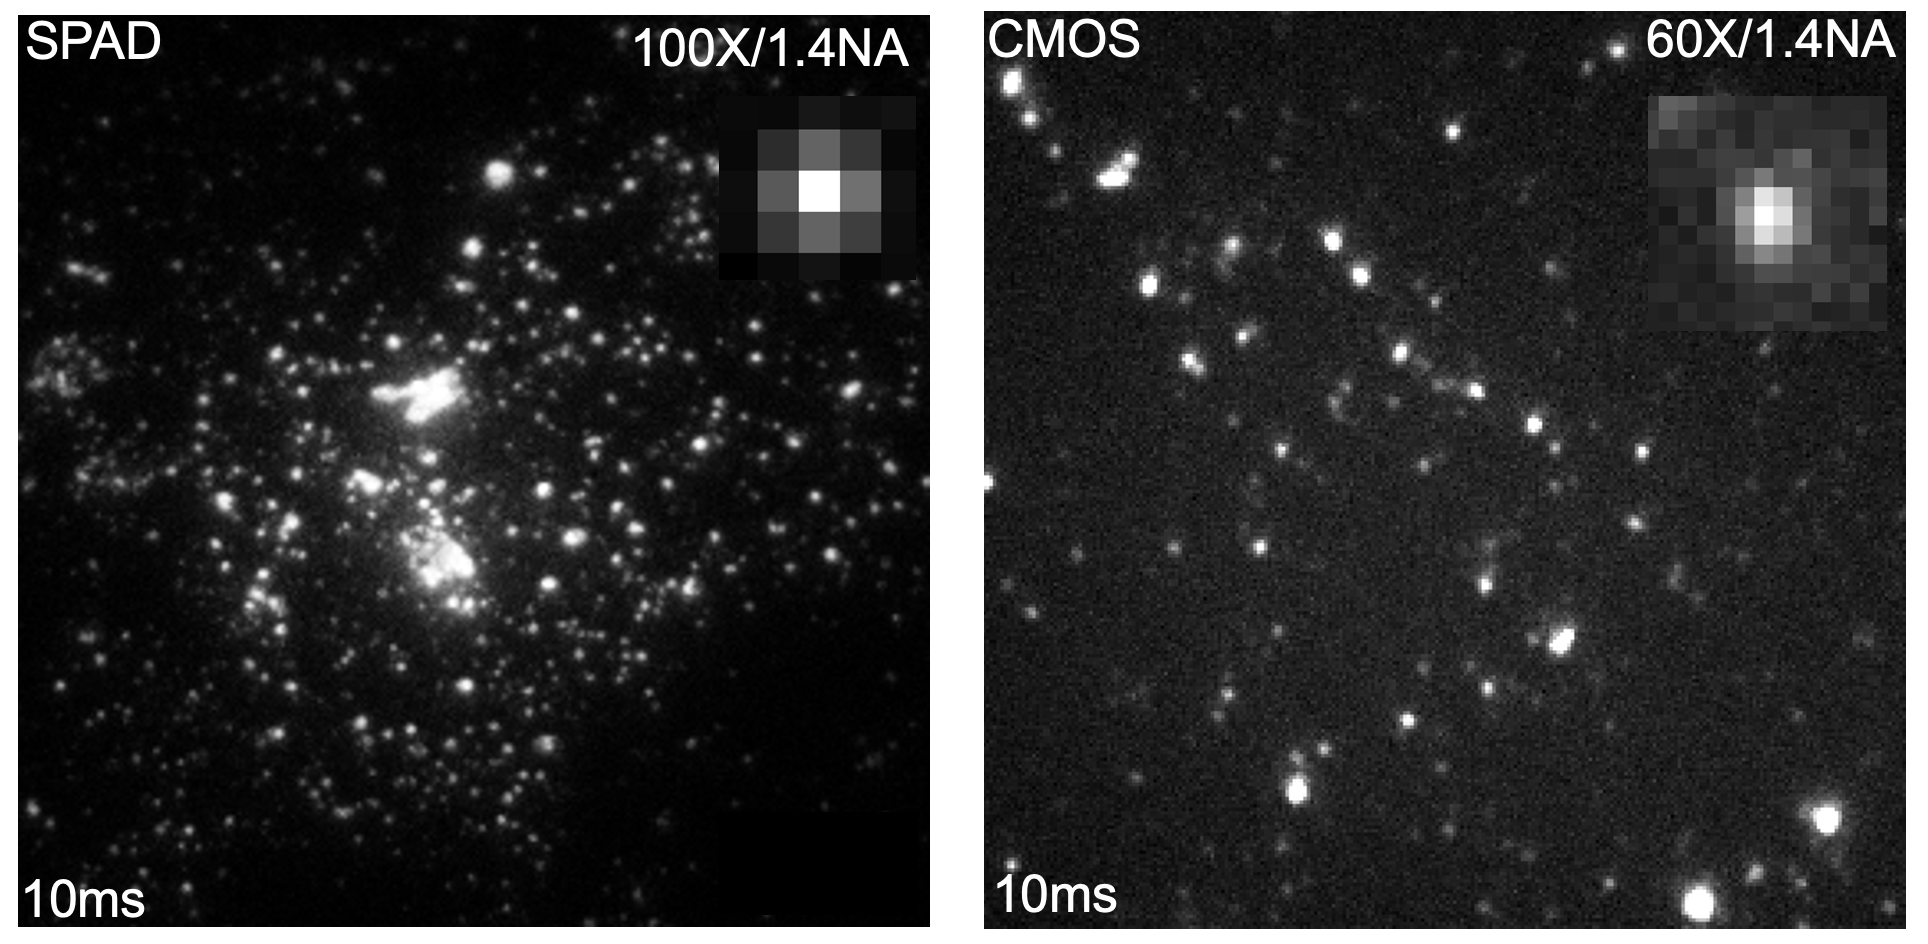
\includegraphics[width=14cm]{/Users/cwseitz/git/cwseitz.github.io/docs/phd/spad/spad/media/SPADvCMOS.png}
\caption{\textbf{Comparison of quantum dot images between CMOS and SPAD cameras}. (left) SPAD image of Qdot655 coated on a glass coverslip using a 100X/1.4NA oil-immersion objective (Nikon) and a 10ms exposure time. (right) CMOS image of Qdot655 using a 60X/1.4NA oil-immersion objective (Olympus) and a 10ms exposure time. Both use continuous-wave 640nm excitation}
\label{fig:fig4}
\end{figure*}    

%Molecular counting with fluorescence antibunching has a fairly simple motivation: coincidence of photons at multiple detector elements during high speed imaging provides evidence for the number of single photon sources present in the imaged region. Combining the ideas of conventional super-resolution approaches with photon statistics may prove to be a powerful set of methods for bioimaging. SPAD cameras achieve orders of magnitude higher temporal resolutions than standard CMOS cameras, single photon sensitivity, and dark count rates less than 25 counts per second (Figure \ref{fig:fig30}). Furthermore, the reduced readout noise and large fill-factor of recently commercialized SPAD arrays suggests their use for single molecule localization with reduced uncertainty.

%Here, we present a method for widefield single photon counting in order to count fluorophores in the sample and subsequently constrain single molecule localization. We investigate the theoretical properties of the zero-lag, second-order coherence function $g^{(2)}(0)$ for widefield photon counting and its spatial properties (Figure \ref{fig:fig5}). Using Bayesian analysis, we derive a posterior distribution on the number of active fluorescent emitters in a region of interest. This result is then combined with single molecule localization algorithms.  We demonstrate resolution of multiple emitters using a multi-emitter fitting algorithm and report localization errors with respect to the CRLB.


\subsection{Results}

\subsubsection{Model}

\begin{figure*}[t]
\centering
\includegraphics[width=16cm]{/Users/cwseitz/git/cwseitz.github.io/docs/phd/spad/spad/media/Figure-0.png}
\caption{\textbf{Single photon counting with a SPAD array} (a) Simplified diagram of the widefield photon counting setup (b) Single photon imaging scheme using 1$\mu$s exposures containing a picosecond laser pulse (c) Sum of photon counts over a 5x5 region of interest (ROI), taken with $N_{\mathrm{frames}}=5\times 10^{5}$}
\label{fig:fig5}
\end{figure*}    

Consider a simplified description of widefield photon counting for a a single photon source in the object plane labeled by a continuous-valued coordinate $\theta=(\theta_u,\theta_v)$. The spatial profile $O$ of the field in image space is again presumed to have a Gaussian shape \parencite{Zhang2007,Richards1959,Gibson1989}. 

\begin{equation}
I(t)=\frac{W(t)}{2\pi\sigma^2}e^{-\frac{\left(u-\theta_u\right)^2+\left(v-\theta_v\right)^2}{2\sigma^2}}  
\end{equation}

In general, fluorescent emission is a doubly stochastic process \parencite{Chen1999}, due to temporal fluctuations in the intensity $W(t)$ as well as the quantum nature of light. We therefore define the molecular brightness $\zeta(t)\propto W(t)$ as the probability a photon is detected from a fluorescent emitter at a time $t$ . All factors that affect the photon count rate, such as laser power, absorption cross section, fluorescence quantum yield, detector efficiency, etc., are absorbed into $\zeta(t)$. Under stationary conditions in which $W(t)$ and $\zeta(t)$ are constants, we write $\zeta(t)=\zeta$. In this case, for an isolated single photon source, the PCH will follow a Bernoulli distribution: 

%A similar theoretical exposition to follows to Section 1.2; however, slight modifications are made to the notation to relate it to the quantum theory. Since our SPAD detectors at the image plane must also be discrete, the intensity at a detector element $k$ centered in image space at $s_k=(u_k,v_k)$ is given by integrating over pixels of width $\delta=1$. Using the definitions of $\Gamma_u,\Gamma_v$ from Section 1.2, we define

%\begin{equation}
%\zeta_{k}\vcentcolon = \langle n_{k} \rangle = \Gamma_{u}(u_k,\theta_u)\Gamma_{v}(v_k,\theta_v)\zeta
%\end{equation}

%where $\langle n_{k} \rangle$ is the expected number of photons detected at pixel $k$. We now consider the case of pulsed excitation where the interval between pulses is much longer than the fluorescence lifetime. Upon excitation of an isolated fluorescent emitter, a photon is detected at a particular detector element $k$ with probability $\zeta_{k}$. Similarly, the probability of detection in a region of interest collecting all photons is $\zeta$. Here, we are primarily concerned with the latter quantity, and its application in counting fluorescent emitters.

\begin{equation}
\mathcal{L}_{\mathrm{signal}}^{(1)}(n_{\mathrm{signal}}\lvert\zeta)\ =\ \mathrm{Bernoulli}(\zeta)
\end{equation}

If N fluorescent emitters are present in the ROI, the PCH will be the $N$-th convolution of the single emitter PCH with itself \parencite{Chen1999}

\begin{equation}
\mathcal{L}_{\mathrm{signal}}(n_{\mathrm{signal}})=\mathcal{L}_{signal}^{(1)}(\zeta_1)\otimes\mathcal{L}_{\mathrm{signal}}^{(2)}(\zeta_2)\otimes\ \cdots\otimes\mathcal{L}_{\mathrm{signal}}^{(N)}(\zeta_N)
\end{equation}

Therefore, for $N$ identical fluorophores emitting photons which can be detected within a ROI of the array, the number of signal photons measured $n_{\mathrm{signal}}$ following a single excitation pulse will have Binomial statistics $n_{\mathrm{signal}}\sim \mathrm{Binom}\left(N,\zeta\right)$. Photon pile-up at a single detector element can be safely neglected in this model due to its relatively low likelihood. Coherent background signal will follow Poissonian statistics $n_{\mathrm{bg}}\sim\mathrm{Poisson}\left(\lambda\right)$ for an expected number $\lambda$ of background counts in the ROI per frame. The total number of counts $n=n_{\mathrm{signal}}+n_{\mathrm{bg}}$ detected in the region of interest following a single pulse is then distributed by the PCH:

\begin{equation}
\mathcal{L}\left(n\mid N,\zeta,\lambda\right)=\mathcal{L}_{\mathrm{signal}}(n_{\mathrm{signal}}\lvert N,\zeta)\otimes\mathcal{L}_{\mathrm{bg}}(n_{\mathrm{bg}}\lvert \lambda)=\sum_{i=0}^{\infty}\binom{N}{i}\zeta^i\left(1-\zeta\right)^{N-i}\frac{\lambda^{n-i}}{\left(n-i\right)!}e^{-\lambda} 
\end{equation}

The expression above represents a convolution of Poisson and Binomial probability mass functions. This result is the primary means of inference of the number of active emitters $N$ in a ROI as well as theoretical analysis of the second-order coherence. 


%\begin{figure}[t]
%\centering
%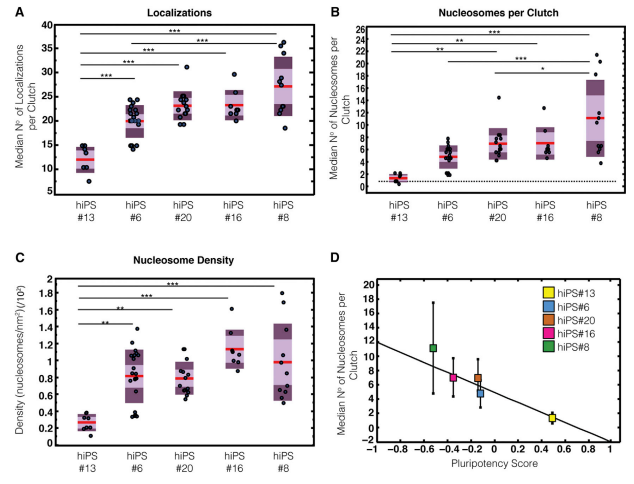
\includegraphics[width=12cm]{/Users/cwseitz/git/cwseitz.github.io/docs/phd/spad/spad/media/Figure-4.png}
%\caption{\textbf{Posteriors on the number of fluorescent emitters $N$ and localization for $N^{*}=1$} (left) and $N^{*}=2$ (right) quantum dots. Scalebars 360nm}
%\label{fig:fig7}
%\end{figure}


%By temporarily ignoring the spatial profile described by (2.3), we derive a likelihood on the number of fluorophores in a small ROI with a lateral dimension $d = 5$ pixels. For $N$ fluorophores emitting photons which can be detected within a ROI of the SPAD array, the number of signal photons measured $n_{\mathrm{signal}}$ following a single excitation pulse will have Binomial statistics $n_{\mathrm{signal}} \sim \mathrm{Binom}(N,\zeta)$. Photon pile-up at a single detector element can be safely neglected in this model due to its relatively low likelihood. We then model the background signal within the ROI as a coherent state, which we have shown follows Poissonian statistics $n_{\mathrm{background}} \sim \mathrm{Poisson}(\lambda)$ for an expected number $\lambda$ of background counts in the ROI, per frame. The total number of counts $n=n_{\mathrm{signal}}+n_{\mathrm{background}}$ detected in the ROI following a single pulse is then distributed by the likelihood

%\begin{equation}
%p(n \mid N,\zeta,\lambda) = \sum_{i=0}^{\infty} \binom{N}{i} \zeta^i (1-\zeta)^{N-i} \frac{\lambda^{n-i}}{(n-i)!} e^{-\lambda}
%\end{equation}

%The expression above represents a convolution of Poisson and Binomial probability mass functions. This result is the primary means of inference of the number of active emitters $N$ in a ROI.

%In order to begin to perform localization in non-sparse ROIs, we write a posterior distribution on the Binomial parameters used in the likelihood, using Bayes rule. Presuming $\lambda$ can be reliably estimated, we have

\subsubsection{Empirical estimation of second-order coherence}

To measure fluorescence antibunching in experiments, the second order coherence function $g^{(2)}(m)$ is used \parencite{Israel2017}. An empirical estimate of $g^{(2)}(m)$ is made, based on the number of coincidences $G^{(2)}(m)$ at a lag time $m$

\begin{equation}
g^{(2)}(m)=\frac{G^{(2)}(m)}{\langle G^{(2)}(m)\rangle }
\end{equation}


The function $G^{(2)}(m)$ counts the number of coincidences at a lag time $m$ and is normalized by its expectation $\langle G^{(2)}(m)\rangle$. It is well known that, for coherent (Poissonian) light, the second order coherence function $g^{(2)}(m)$ is approximately unity for all lags $m$. This is not necessarily the case, however, for binomial states \parencite{Stoler1985} of the quantized radiation field. To investigate the properties of the $g^{(2)}(0)$ dip for binomial photon statistics, we compared the expected number of coincidences at zero-lag $G^{(2)}(0)$ as well as the $g^{(2)}(0)$ value for purely binomial or Poissonian photon statistics, with the same mean. As expected, we found that binomial statistics gave a dip below $g^{(2)}(0) =0.5$ for small fluorophore numbers while Poissonian statistics gave a value of $g^{(2)}(0) =0.5$ (Figure \ref{fig:binomvpoiss}a). This result was also seen for pure binomial statistics (zero background signal) over a range of $\zeta$ values (Figure \ref{fig:binomvpoiss}b). For nonzero background signal, we find that the signal to background ratio becomes relevant, with decreasing $\zeta$ values raising the expected dip to $g^{(2)}(0) =0.5$ (Figure \ref{fig:binomvpoiss}c).


\subsubsection{Bayesian inference of the number of active emitters}

When the number of fluorescent emitters $N$ is unknown, the PCH (likelihood function) can be used in a Bayesian inference scheme to construct a posterior distribution on the binomial parameters:

\begin{equation}
p(N,\zeta\lvert n) \propto p(n\lvert N,\zeta)p(\zeta)
\end{equation}

We use a Gaussian prior on $\zeta$, i.e. $p(\zeta) = \mathcal{N}(\mu_{\zeta},\sigma_{\zeta}^2)$. Prior uncertainty in the value of $\zeta$ stems from fluorophores with potentially complex photophysical properties. This posterior can be integrated over $\zeta$ to produce a posterior distribution on the fluorophore number $N$. That is, $p(N=N'\lvert n) \propto \int_{0}^{1} \mathcal{L}(n\lvert N',\zeta)p(\zeta) d\zeta$ for $\mathcal{L}(n\lvert N',\zeta)=\prod_{j=1}^{N\mathrm{frames}} p(n_{j}\lvert N',\zeta)$. The likelihood is made tractable by a log-sum-exponential trick: $\mathcal{L}(n\lvert N',\zeta) = e^{\left(\sum_{j}\ell (n_{j}\lvert N',\zeta) + C\right)}$, where $C$ is an arbitrary constant determined empirically. This same constant $C$ is used for all $N'$. Monte Carlo integration is then employed to integrate out $\zeta$. This involves sampling many $\zeta$ values from the Gaussian prior and, for each sampled $\zeta$, the Poisson-Binomial likelihood $\mathcal{L}(n\lvert N',\zeta)$ is computed. These likelihood values are then weighted by the prior probabilities $p(\zeta_i)$. The final result is obtained by averaging these weighted likelihoods over all sampled $\zeta$, which approximates the integral:

\begin{equation}
p(N=N'\lvert n) = \int_{0}^{1} \mathcal{L}(n\lvert N',\zeta) p(\zeta) \, d\zeta \approx \frac{1}{S} \sum_{i=1}^S \mathcal{L}(n\lvert N',\zeta_i) p(\zeta_i)
\end{equation}

where $S$ is the number of samples from the prior. This method provides a powerful way to handle the integration of complex or high-dimensional functions, especially when analytical solutions are intractable. The final posterior can then be estimated by minibatching the data and averaging the posterior $p(N\lvert n)$ over minibatches. An estimate of the fluorophore number $N$ within each ROI is found by the maximum aposteriori (MAP) estimate $N^{*}$ given by this distribution.

%For localization, we notice that the Poisson-Binomial likeliood is well approximated by a Poisson distribution for $\zeta << 1$, making the localization procedure similar to conventional maximum likelihood methods discussed in Chapter 1. Therefore, we have the following log-likelihood on the image $\bold{x}$:


%\begin{equation}
%\ell(\bold{x}\lvert \theta) = -\log \prod_{k} \frac{e^{-\left(\mu_{k}\right)}\left(\mu_{k}\right)^{n_k}}{n_k!}\\
%= \sum_{k}  \log n_k! + \mu_{k} - n_k\log\left(\mu_{k}\right)
%\end{equation}

%\begin{figure*}[t]
%\centering
%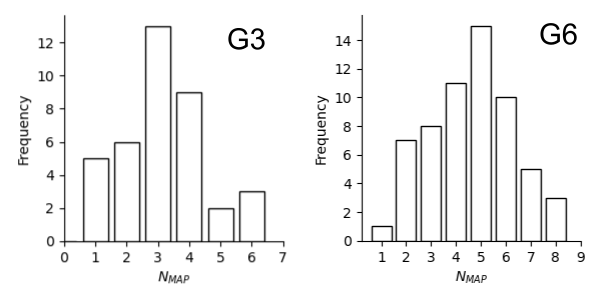
\includegraphics[width=12cm]{/Users/cwseitz/git/cwseitz.github.io/docs/phd/spad/spad/media/Figure-5.png}
%\caption{\textbf{Single and multi-emitter localization error on sums of photon counts}. (left) Localization uncertainty for simulated data for different values of $N$, plotted with respect to the Cramer-Rao lower bound, shown in dashed gray. (right) Multi-emitter localization by MCMC sampling for $N=3$, colors indicate a cluster of samples i.e., a single localization. All data was generated with a background rate $\langle n_{\mathrm{background}} \rangle = \lambda N_{\mathrm{frames}}/d^{2}$ per pixel. Scalebar 360nm}
%\label{fig:fig6}
%\end{figure*}   

%where, in the multi-emitter regime the expected photon count at a pixel is $\mu_{k} = \sum_{m=1}^{N^{*}} \mu_{k,m}$ and $\mu_{k,m}=\zeta N_{\mathrm{frames}}\Gamma_{x}(u_k,\theta_{u,m})\Gamma_{y}(v_k,\theta_{v,m}) + \lambda N_{\mathrm{frames}}/d^{2}$. In the multi-emitter regime, optimization of the likelihood can be more challenging, and sampling is a more suitable choice compared to gradient-based methods (see Results). 

\subsubsection{Simulations}

\begin{figure}
\centering
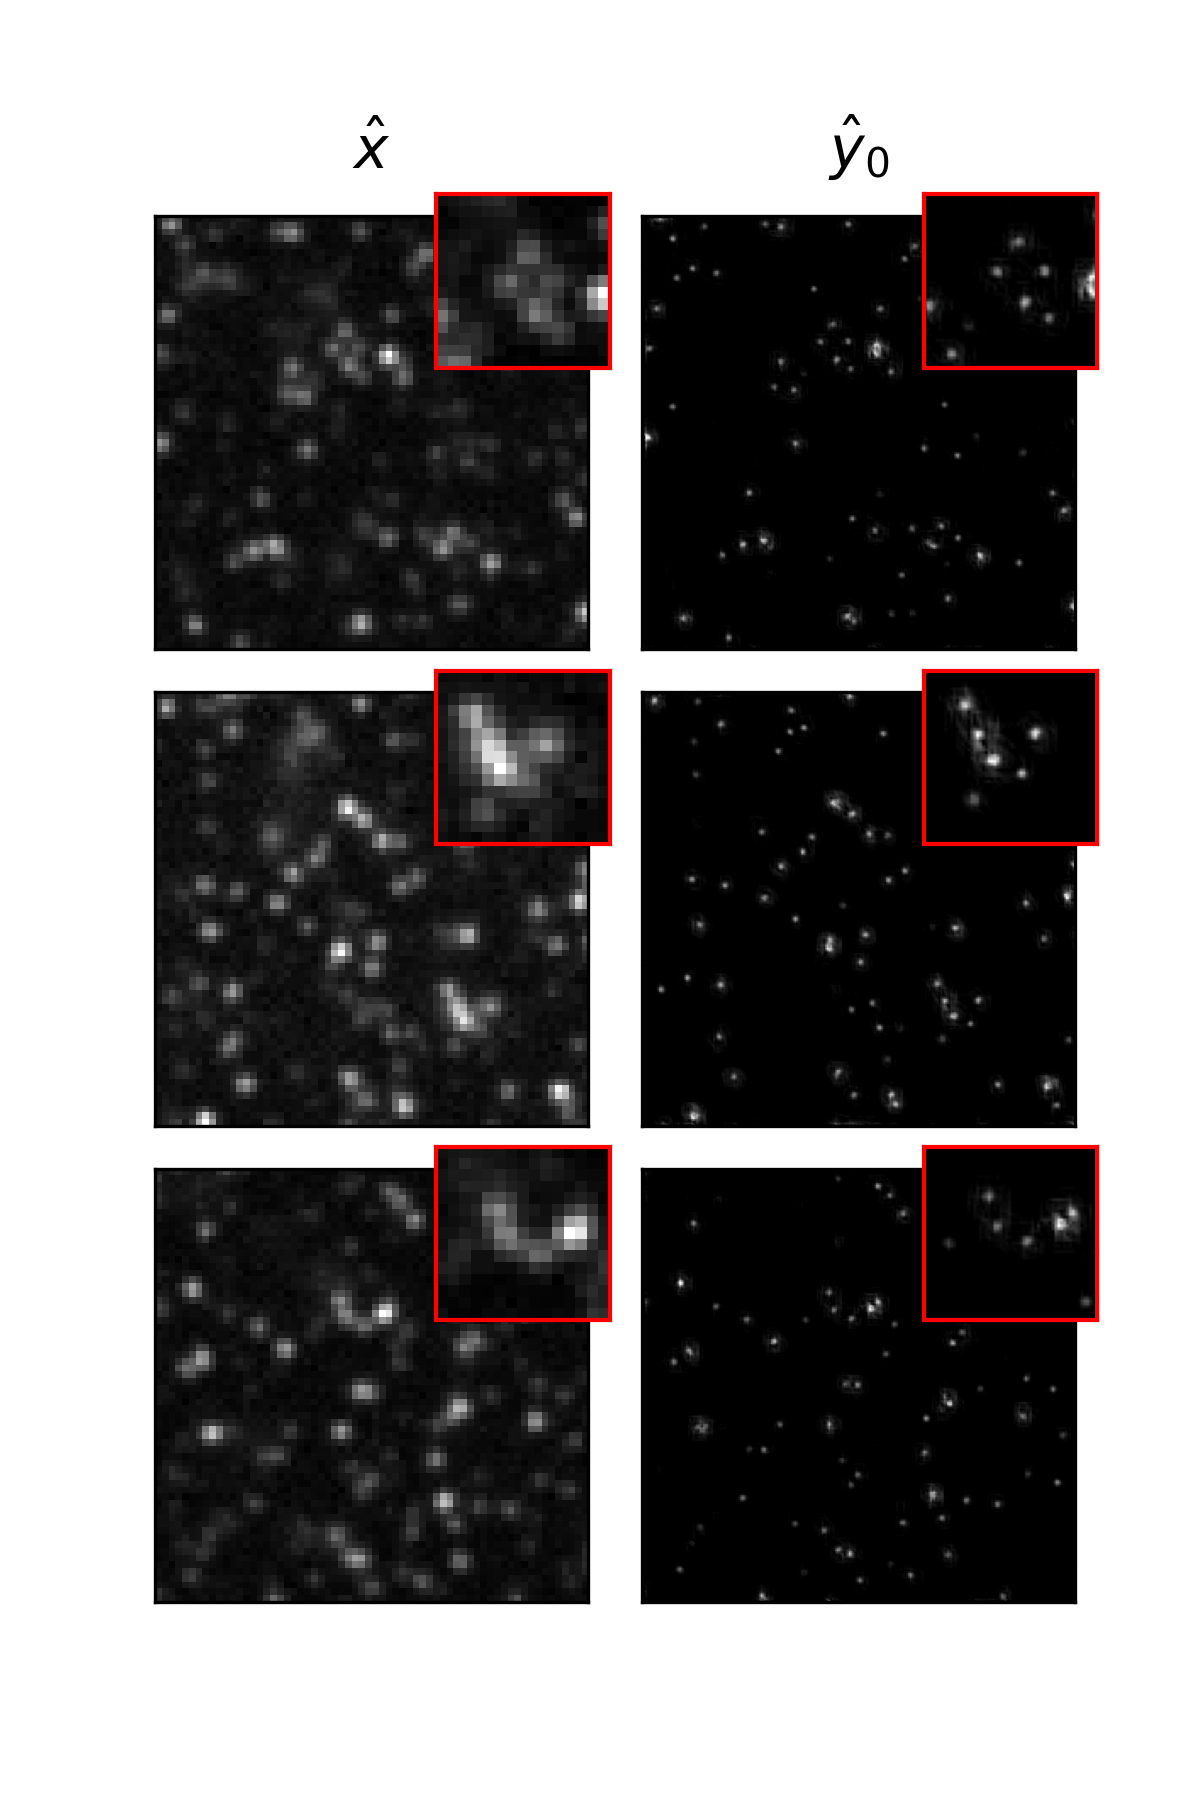
\includegraphics[width=16cm]{/Users/cwseitz/git/cwseitz.github.io/docs/phd/spad/spad/media/Figure-6.png}
\caption{\textbf{Photon counting histogram and analysis on zero-background simulations} (a) Simulated photon counts in 1us exposure for N=1 and $\zeta=0.01$ (b) Photon counting histogram for counts in (a) (c) Second-order coherence function for data in (a) (d) Posterior distribution for data in (a). (e) Simulated photon counts in 1us exposure for N=1 and $\zeta=0.01$ (f) Photon counting histogram for counts in (e) (g) Second-order coherence function for data in (e) (h) Posterior distribution for data in (e). (i) Simulated photon counts in 1us exposure for N=1 and $\zeta=0.01$ (j) Photon counting histogram for counts in (i) (k) Second-order coherence function for data in (i) (l) Posterior distribution for data in (i). Inference in (d,h,l) use $\mu_\zeta=0.01,\sigma_\zeta=0.001$}
\label{fig:pch}
\end{figure}  

To validate our model, we apply it on the simulated photon emissions from single and multiple quantum emitters. Simulated photon count time-series were generating by sampling from the Poisson-Binomial PCH described using variable values for $N$ and $\zeta=0.01$ (Figure \ref{fig:pch}a,e,i). As expected, we found that $g^{(2)}(0)<0.5$  while for increasing values of $N$, $g^{(2)}(0)$ approached $g^{(2)}(0)=0.5$ (Figure \ref{fig:pch}c,g,k). Analysis of the posterior distribution on $N$ successfully recovered the value of $N$ used to parameterize simulations (Figure \ref{fig:pch}d,h,l). 

\subsubsection{Distinguishing single quantum dots from assemblies}

A custom widefield fluorescence microscope was built for widefield photon counting by synchronization of laser pulses with 1-bit exposures of a SPAD array. This excitation scheme permits the computation of the second order coherence function  $g^{(2)}(m)$ and visualization of the spatial intensity distribution by summing photon counts over time. The acquisition scheme and analytical methods were then applied in two experimental contexts. First, we examined the posterior distribution and $g^{(2)}(m)$ function for putatively isolated quantum dots and then examined quantum dot aggregates. Quantum dots exhibit temporally heterogeneous photoluminescence (PL) due to nonradiative transitions of electrons in the conduction band giving rise to a phenomenon known as blinking \parencite{Stoler1985,Furuta2022}. Quantum dots showing clear two-state PL fluctuations exhibited $g^{(2)}(0)<0.5$ and a posterior distribution maximized at $N=1$ (Figure \ref{fig:qdagg}a-d). Aggregates of quantum dots with more complex PL fluctuations showed $g^{(2)}(0)=0.5$ and a posterior distributed around larger values of $N$ (Figure \ref{fig:qdagg}e-h) 

\begin{figure}
\centering
\includegraphics[width=16cm]{/Users/cwseitz/git/cwseitz.github.io/docs/phd/spad/spad/media/Figure-1.png}
\caption{\textbf{Distinguishing single and multiple quantum dots} (a) Photon counts in 1us exposure using 532nm pulsed excitation of a putatively isolated QD (b) Photon counts in 10ms exposure using 488nm continuous-wave excitation (c) Second-order coherence function for data in (a) (d) Posterior distribution for data in (a) (e) Photon counts in 1us exposure using 532nm pulsed excitation of a QD aggregate (f) Photon counts in 10ms exposure using 488nm continuous-wave excitation (g) Second-order coherence function for data in (e) (h) Posterior distribution for data in (e). Inference parameters can be found in Table 1.}
\label{fig:qdagg}
\end{figure}  

\clearpage
\begin{figure}
\centering
\includegraphics[width=16cm]{/Users/cwseitz/git/cwseitz.github.io/docs/phd/spad/spad/media/Figure-3.png}
\caption{\textbf{Counting ATTO532 dye bound to DNA origamis}. (a) Example DNA origami with three ATTO532 binding sites. (b) Photon counts in 1us exposure using 532nm pulsed excitation of G3 sample and sum of counts (inset). (c) Second order coherence for the spot in (b). (d) Posterior distribution for the spot in (b). (e) Example DNA origami with three ATTO532 binding sites. (f) Photon counts in 1us exposure using 532nm pulsed excitation of G3 sample and sum of counts (inset). (g) Second order coherence for the spot in (f). (h) Posterior distribution for the spot in (f). (i) Example DNA origami with six ATTO532 binding sites (G6 sample). (j) Photon counts in 1us exposure using 532nm pulsed excitation of G6 sample and sum of counts (inset). (k) Second order coherence for the spot in (j). (l) Posterior distribution for the spot in (j).}
\label{fig:atto}
\end{figure}  

\clearpage
\begin{figure}
\centering
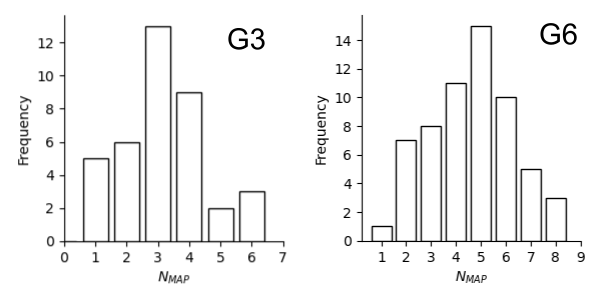
\includegraphics[width=12cm]{/Users/cwseitz/git/cwseitz.github.io/docs/phd/spad/spad/media/Figure-5.png}
\caption{\textbf{Distributions of the maximum aposteriori estimate of N} (left) Distribution of estimate of N for DNA origamis with three ATTO532 binding sites (G3 sample) (right) Distribution of estimate of N for DNA origamis with six ATTO532 binding sites (G3 sample). Prior mean set to $\mu_\zeta=0.002$ for both G3 and G6 samples.}
\label{fig:atto2}
\end{figure}  

\subsubsection{Counting fluorophores bound to DNA origamis}


In a second series of experiments, we examined the posterior distribution and $g^{(2)}(m)$ function for DNA origamis which can bind up to $N=3$ or $N=6$ ATTO532 fluorescent dye molecules, referred to as G3 and G6, respectively (Figure \ref{fig:atto}a,f,j) For origamis which can bind up to $N=3$ ATTO532 dyes, no clear $g^{(2)}(0)$ dip was observed, due to the low signal to background ratio at this signal level (Figure \ref{fig:atto}c,g). For origamis which can bind up to $N=6$ ATTO532 dyes, no clear $g^{(2)}(0)$ dip was observed, due to the large $N$ character of the $g^{(2)}(0)$ dip predicted by the theory (Figure \ref{fig:atto}k). We conclude that the $g^{(2)}(0)$ dip may lead to ambiguous interpretations at low signal levels. However, the posterior distribution can recover the known $N$ value from the photon count distribution for G3 (Figure \ref{fig:atto}d,h) and G6 (Figure \ref{fig:atto}l). Maximum aposteriori (MAP) estimates of the fluorophore number showed consistency with the known value of $N$ for G3 and G6 (Figure \ref{fig:atto2}). 

\clearpage
\begin{table}
\centering
\begin{tabular}{lccccc}
\multicolumn{6}{c}{\textbf{Table 1 - Posterior Parameters}} \\ \hline
\multicolumn{1}{c}{\textbf{Sample}}  & $\mu_{\zeta}$ & $\sigma_{\zeta}$ & $\lambda$ & Samples & Batches \\
Qdot655 & 0.01 & 0.005 & 0.008 & 100 & 50 \\
ATTO532 & 0.002 & 0.001 & 0.006 & 100 & 50 \\
\end{tabular}
\end{table}

\section{Materials and Methods}

\subsection{Quantum dots and DNA origamis preparation}

Fluorescent samples used here were either Quantum dots (Qdot655, ThermoFisher) coated on a glass coverslip, or ATTO532 tagged DNA origamis (GATTAquant). Fluorophores in a region with quasi-uniform laser power were selected for analysis to simplify the prior distribution on the molecular brightness. DNA origami samples contained origamis with either three or six ATTO532 binding sites for testing the Bayesian inference scheme and second-order coherence analysis. 

\subsection{Single molecule imaging with the SPAD array}

A 512x512 Fluorescent SPAD512 array (Pi Imaging Technologies) was connected to the customize-built single molecule imaging system (ASI). A picosecond 532nm pulsed laser (Picoquant) was triggered at 500 KHz as the excitation source. Laser power was set at 300uW at the back focal plane of the microscope objective for all experiments. Emission light was collected using an oil-immersion 100X/1.4NA objective (Nikon). The emission signal was filtered to exclude the laser line (Semrock) and projected onto the SPAD512 sensor using a tube lens. The acquisition of the SPAD assay is synchronized with the pulsed laser frequency. Each acquisition consists of a series of 1-bit frames, using a 1us exposure per frame. For quantum dot imaging, 30ms total exposure was used (30k frames). For DNA origami imaging, 100ms total exposure was used (100k frames). To obtain time-course data of photon counts, we (i) summed binary images over the entire acquisition (ii) estimated spot centroids using the Laplacian of Gaussian (LoG) detection algorithm, and (iii) extracted total counts in a 5x5 pixel region of interest around each detected spot. 


%Quantum dots coated on a glass coverslip were excited using a picosecond $532\mathrm{nm}$ pulsed laser triggered at $500\mathrm{kHz}$. Emission light was collected using an oil-immersion 100$\times$ objective with numerical aperture (NA) 1.4 (Nikon). The emission signal was then filtered to exclude the laser line (Semrock) and projected onto the SPAD512 sensor (Pi Imaging Technologies) using a tube lens. A simplified diagram of the complete system is depicted in (Figure \ref{fig:fig5} a). Each acquisition consists of $N=5\times 10^{5}$ frames, synchronized with each laser pulse, using a $1\mathrm{us}$ exposure per frame (Figure \ref{fig:fig5} b,d). Example posteriors and multi-emitter fitting on experimental quantum dot data are found in (Figure \ref{fig:fig7}). To measure fluorescence antibunching in the sample, we investigated properties of the zero-lag second order coherence function $g^{(2)}(0)$. The following empirical estimate of $g^{(2)}(0)$ is used \parencite{Israel2017}

%\begin{equation}
%g^{(2)}(0) = \frac{G^{(2)}(0)-B}{\langle G^{(2)}(m\neq 0)\rangle -B}
%\end{equation}

%\begin{figure}[t]
%\centering
%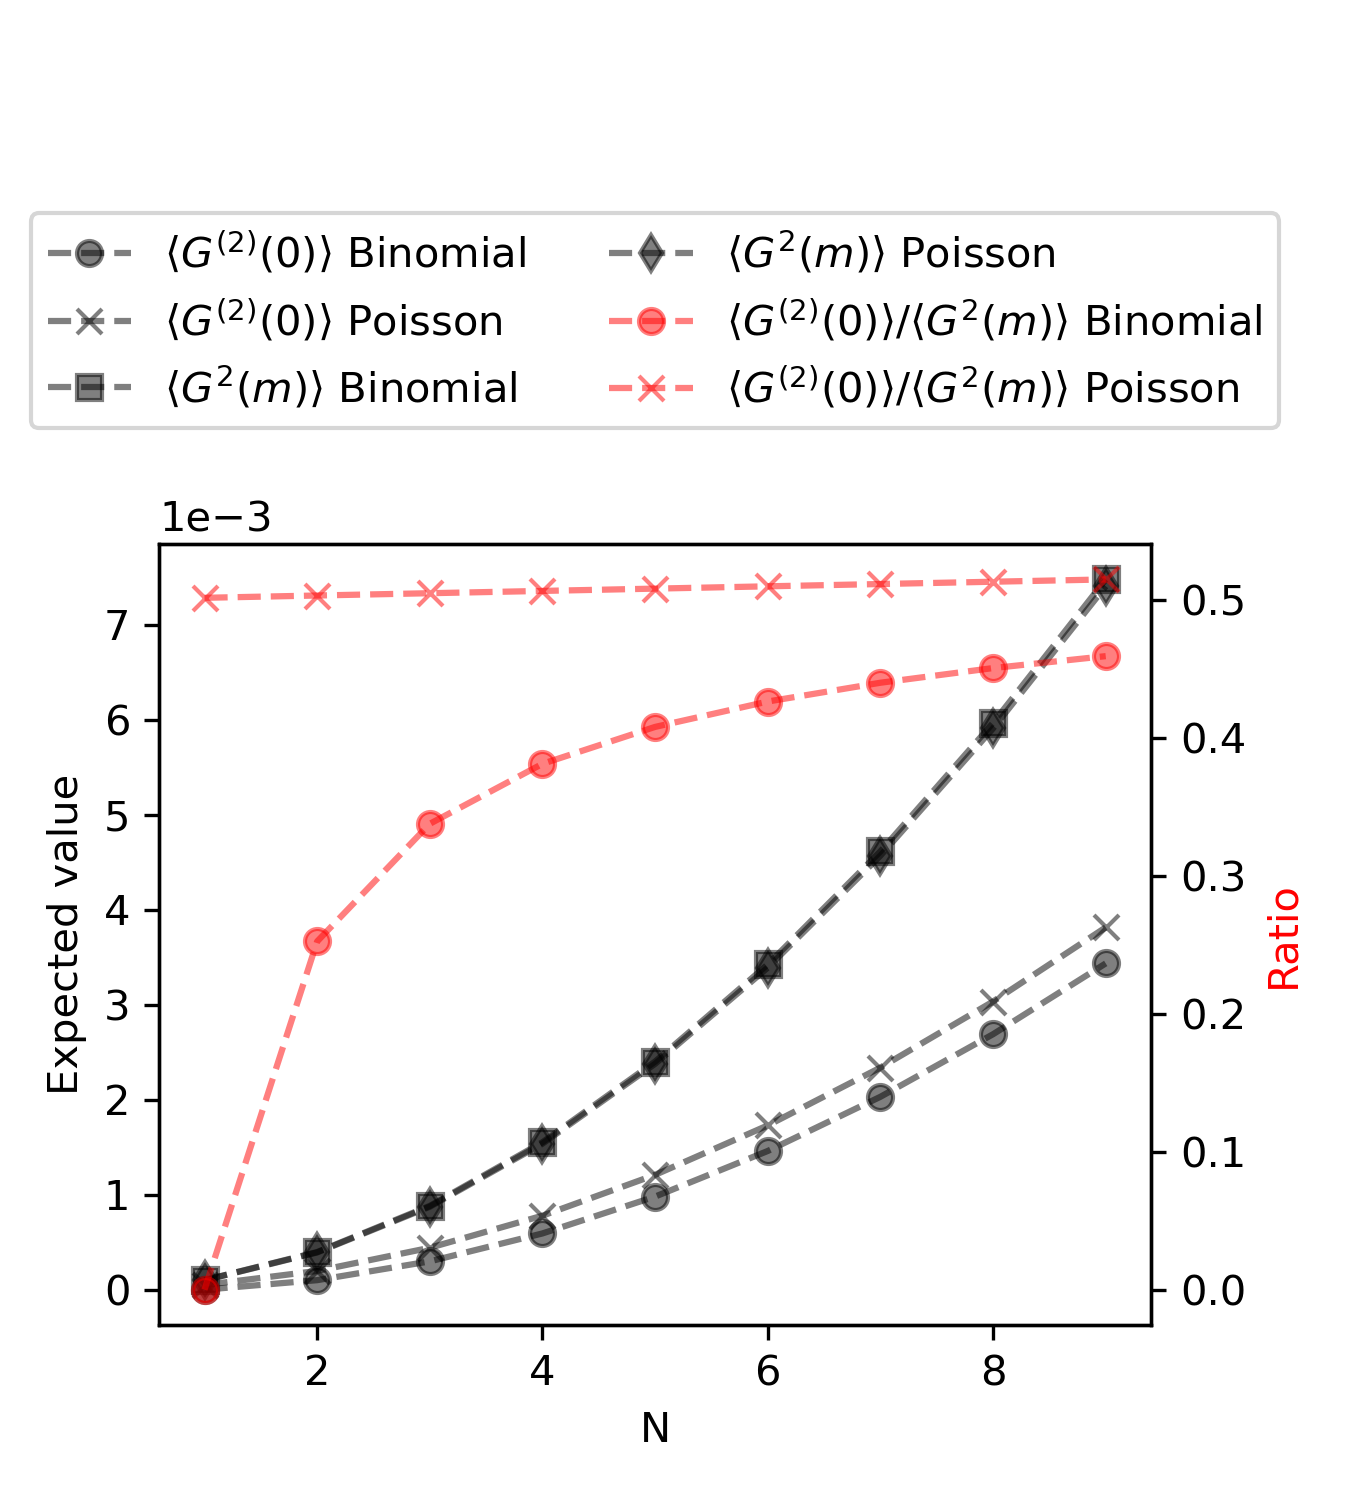
\includegraphics[width=12cm]{/Users/cwseitz/git/cwseitz.github.io/docs/phd/spad/spad/media/binomvpoiss.png}
%\caption{\textbf{Discrepancy of $g^{(2)}(0)$ for pure Binomial or Poissonianian data}. Binomial and Poisson distributions are similar for small $\zeta$ and large $N$. However, for small $N$, the Binomial $g^{(2)}(0)$ deviates from the Poisson $g^{(2)}(0)$ due to a small reduction in $\langle G^{(2})(0)\rangle$ (probability of zero-lag coincidence) in the Binomial case.}
%\label{fig:binomvpoiss}
%\end{figure}   

%\begin{figure}[t]
%\centering
%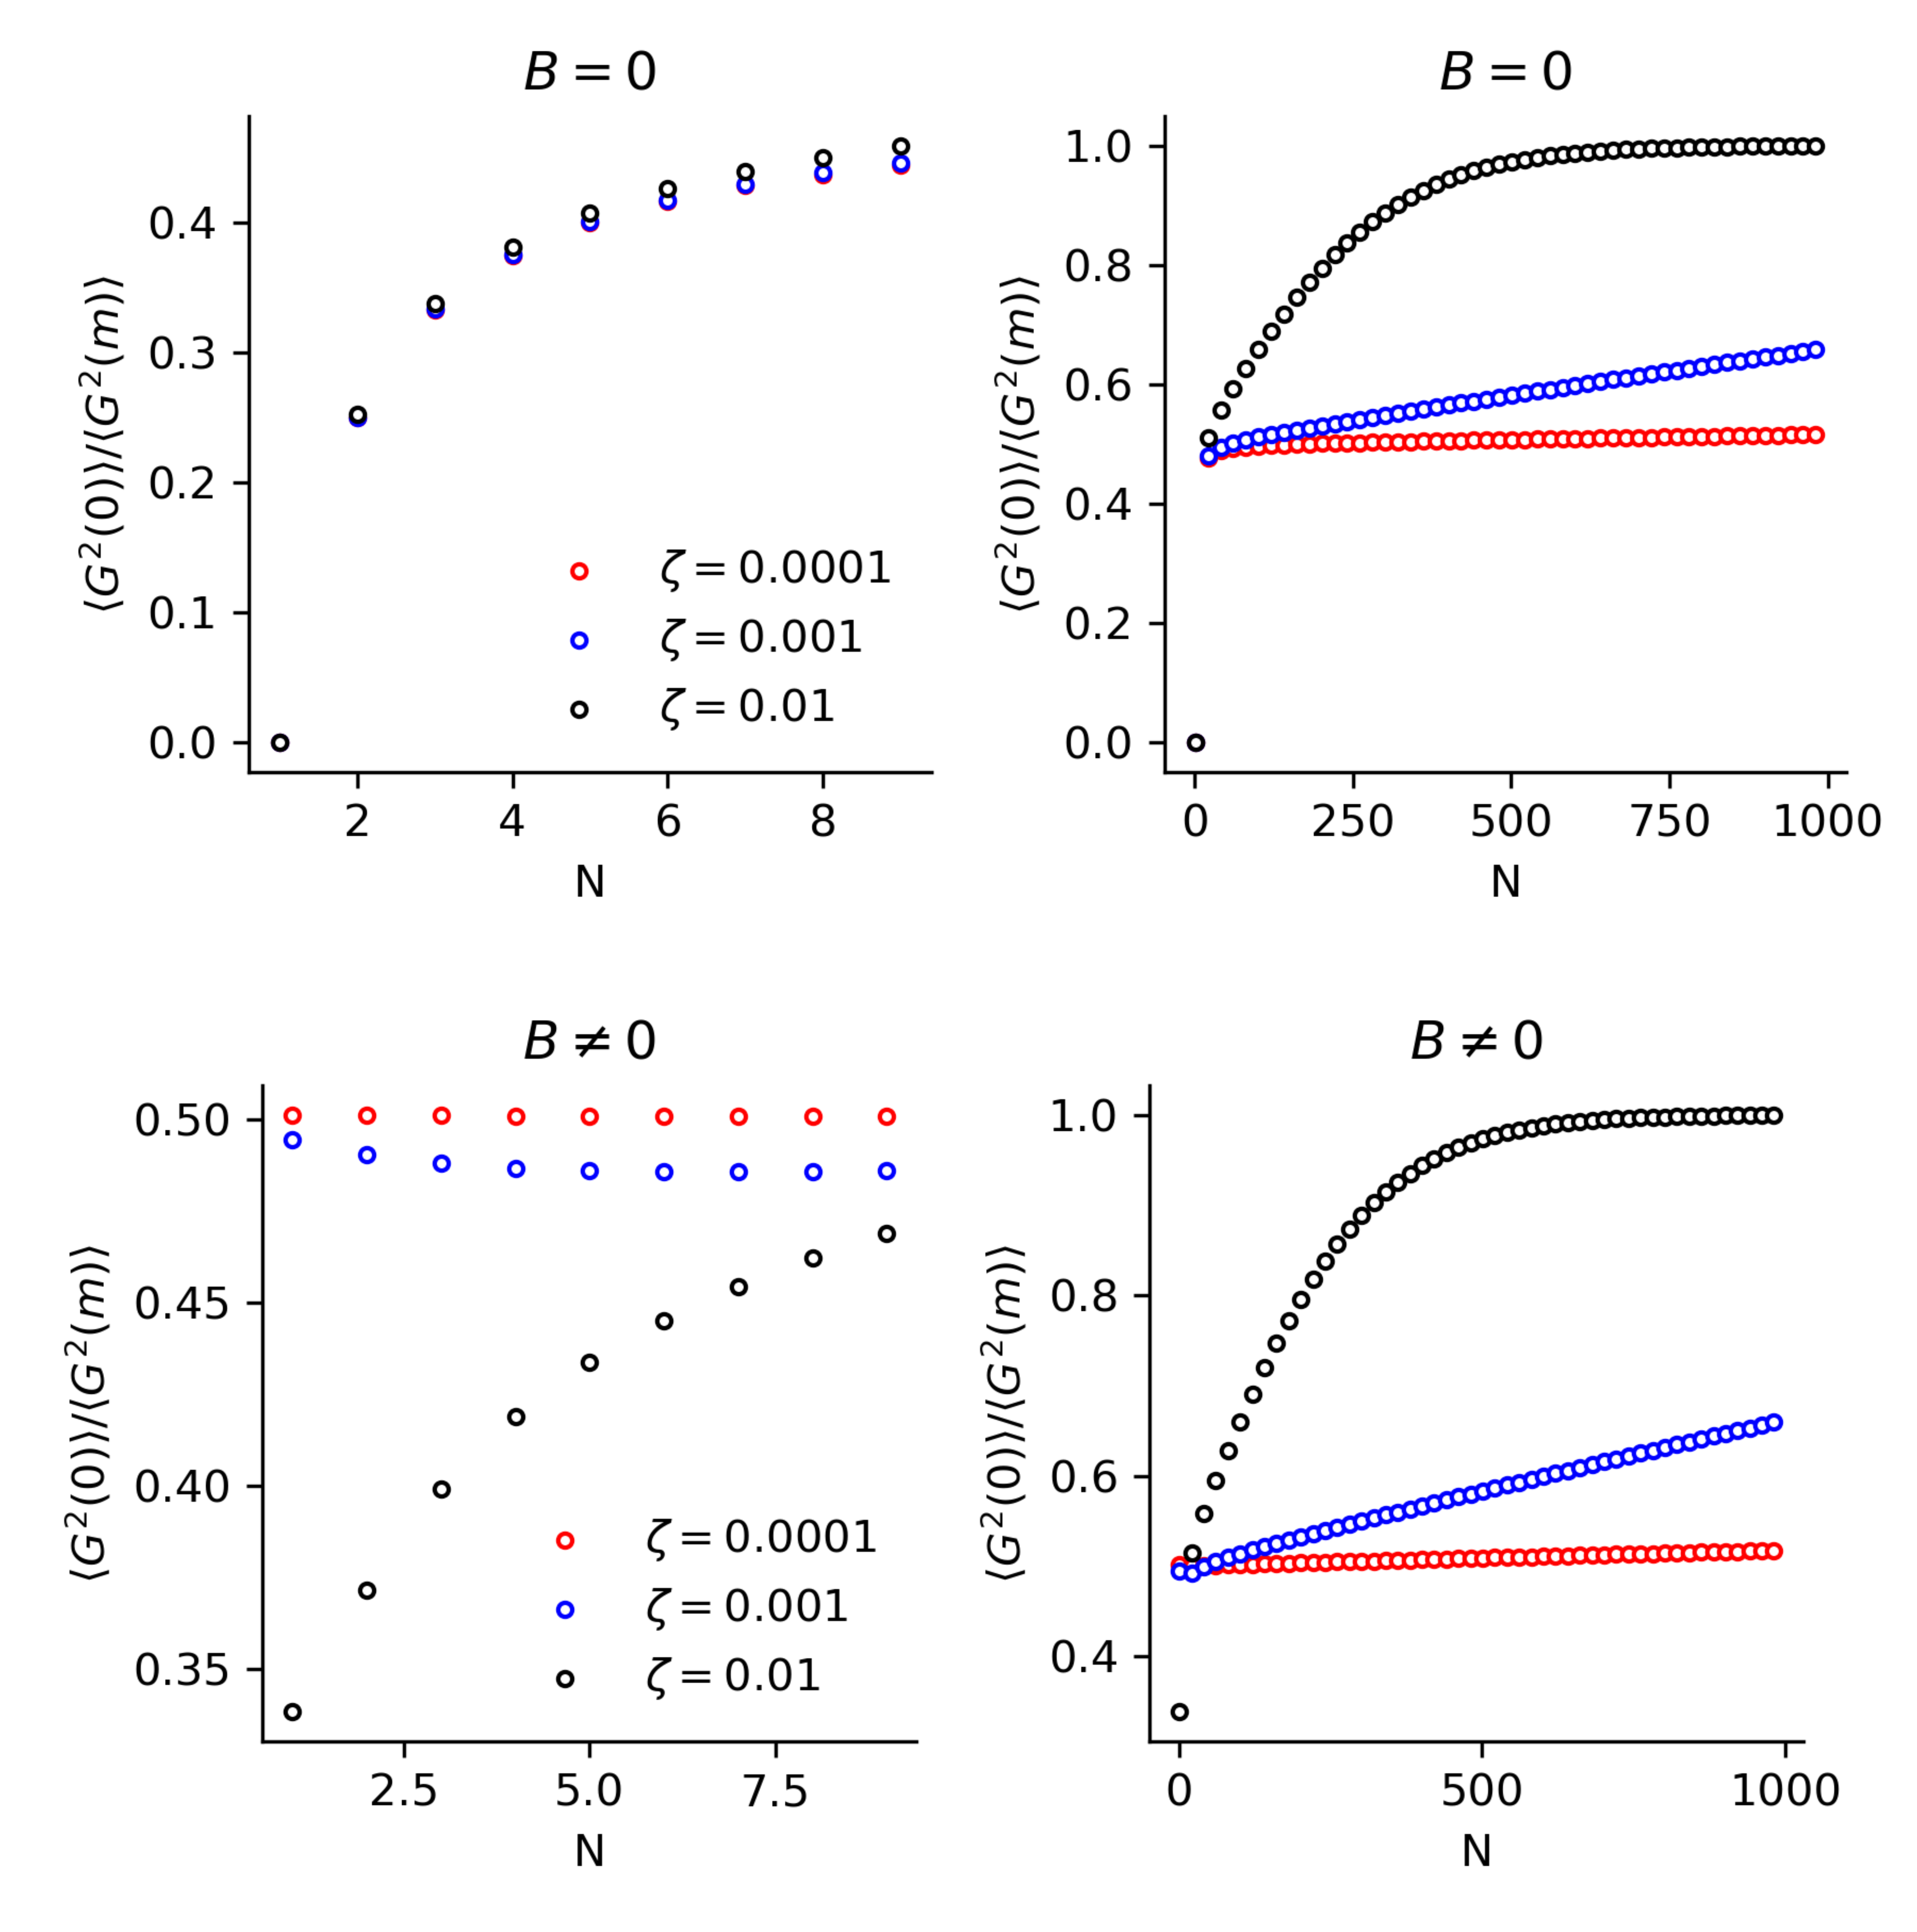
\includegraphics[width=12cm]{/Users/cwseitz/git/cwseitz.github.io/docs/phd/spad/spad/media/g20g2m_full.png}
%\caption{\textbf{Theoretical scaling of $g^{(2)}(0)$ under zero and non-zero background conditions without correction}. (left) Scaling of $g^{(2)}(0)$ for small $N$. (right) Scaling of $g^{(2)}(0)$ for large $N$. For non-zero background conditions, $\lambda = 0.0075$. For small $\zeta$, $g^{(2)}(0)\approx 0.5$, which is the value for Poisson statistics}
%\label{fig:fig8}
%\end{figure}   

%where $B = N_{\mathrm{frames}}\lambda\zeta$ is the expected number of background-signal coincidences in the region of interest. The quantity $G^{(2)}(m)$ represents the number of signal-signal coincidences in the region of interest at a lag time $m$. The quantity $\langle G^{(2)}(m\neq 0)\rangle$ is the average number of coincidences in pairs of frames at nonzero lag $m \in [1,100]$, in units of frames. Averaging $G^{(2)}(0)$ over many realizations (sequences of $N_{\mathrm{frames}}$), gives the expected value $\langle G^{(2)}(0)\rangle $

%\begin{equation}
%\langle G^{(2)}(0)\rangle = N_{\mathrm{frames}}(1 - (1-\zeta)^N - N\zeta (1-\zeta)^{N-1})
%\end{equation}

%Since $G^{(2)}(m)$ is already averaged over $m$, $\langle G^{(2)}(m) $ is effectively a constant over realizations, and must be

%\begin{equation}
%\langle G^{(2)}(m)\rangle =  N_{\mathrm{frames}} \left(1 - \left((1-\zeta)^N\right)\right)^2
%\end{equation}

%Ignoring the effect of background signal $\langle g^{(2)}(0)\rangle =\langle G^{(2)}(0)\rangle/\langle G^{(2)}(m)\rangle$, which rapidly approaches $1/2$ as a function of $N$, and then saturates and slowly while approaching a maximum value of 1 (Figure \ref{fig:fig8}). This is consistent with the idea that for very large number of active fluorescent emitters, the statistics should become Poisson. Lastly, $G^{(2)}(0),G^{(2)}(m),B$ all will have Binomial statistics, which can approximated as Poisson for $\zeta << 1$. Error estimates are then $\delta G^2(0) = \sqrt{G^2(0)}, \delta E(G^2(m)) = \sqrt{\frac{\mathbb{E}(G^2(m))}{M}}, \delta B = \sqrt{B}$. This gives the following error in the value of $g^{(2)}(0)$:

\subsection{Computation of the second order coherence}

In practice, we compute the second order coherence at zero lag using

\begin{equation*}
G^{(2)}(0) =\ \sum_{t}{\mathbb{I}(n_t>1)}
\end{equation*}

where $\mathbb{I}$ is an indicator function. The value of this function at nonzero lag $m$ is given by

\begin{equation*}
G^{(2)}(m) =\ \sum_{t}{\mathbb{I}(n_t n_{t+m}\geq1)}
\end{equation*}

The second order coherence $g^{(2)}(m)$ is then computed over a range $-m_{min}\le m\le m_{max}$. Theoretical estimates of $g^{(2)}(0)$ can be obtained by determining the generating model of $G^{(2)}(m)$. We find that for a sequence of $M$ frames,

\begin{equation*}
G^{(2)}(0)\sim \mathrm{Binomial}(M,p)\ \ \ \ p=\sum_{n\geq2}{\mathcal{L}(n\lvert N,\zeta)}
\end{equation*}

\begin{equation*}
G^{(2)}(m)\sim \mathrm{Binomial}\left(M,q\right)\ \ \ \ \ q=\left(\sum_{n\geq1}{\mathcal{L}(n\lvert N,\zeta)}\right)^2
\end{equation*}

Fluorescence antibunching is conventionally characterized by a dip in the $g^{(2)}(m)$ function for $m=0$, indicating a reduced coincidence probability. Error in the estimate of $g^{(2)}(0)$ are found by the expression


\begin{equation}
\sigma = \text{RMSE}[g^{(2)}(0)] = \sqrt{
    \left[
    \frac{\partial g^{(2)}(0)}{\partial \langle G^{(2)}(m) \rangle} \delta \langle G^{(2)}(m) \rangle
    \right]^2 +
    \left[
    \frac{\partial g^{(2)}(0)}{\partial G^{(2)}(0)} \delta G^{(2)}(0)
    \right]^2
}
\end{equation}

One can then integrate a Gaussian with this $\sigma$ below a threshold e.g, $g^{(2)}(0)=0.5$ to obtain the confidence interval. Lastly, $G^{(2)}(0),G^{(2)}(m)$ will have Binomial statistics, which we approximate as Poisson for simplicity. Error estimates are then $\delta G^2(0) = \sqrt{G^2(0)}, \delta \langle G^2(m)\rangle = \sqrt{\frac{\langle G^2(m)\rangle}{M}}$.This expression simplifies considerably in the case that $\delta \langle G^{(2)}(m)\rangle$ i.e., certainty in $G^{(2)}(m)$. 

\begin{equation}
\sigma_{g^{(2)}(0)}=\sqrt{\frac{p(1-p)}{M q^{2}}}
\end{equation}

The value of $\sigma_{g^{(2)}(0)}$ is therefore a function of $\zeta$ as well as the number of frames in the acquisition $M$. 



%For localization, we use Goodman and Weare's Markov Chain Monte Carlo (MCMC) algorithm \parencite{Goodman2010} to sample from the posterior on fluorophore locations. In all simulations we assume a uniform prior on coordinates over the ROI and $\zeta$ is known and identical over fluorophores. Fluorophore locations can then be estimated from the posterior samples by K-means clustering of the $(\theta_u,\theta_v)$ coordinates of the first particle and identification of cluster centers. To validate our estimator, we compare its RMSE to the single emitter CRLB. We find that for thousands of expected signal photon counts, localization uncertainty lies in an acceptable range for localization microscopy (Figure \ref{fig:fig6}).



%\begin{figure}
%\centering
%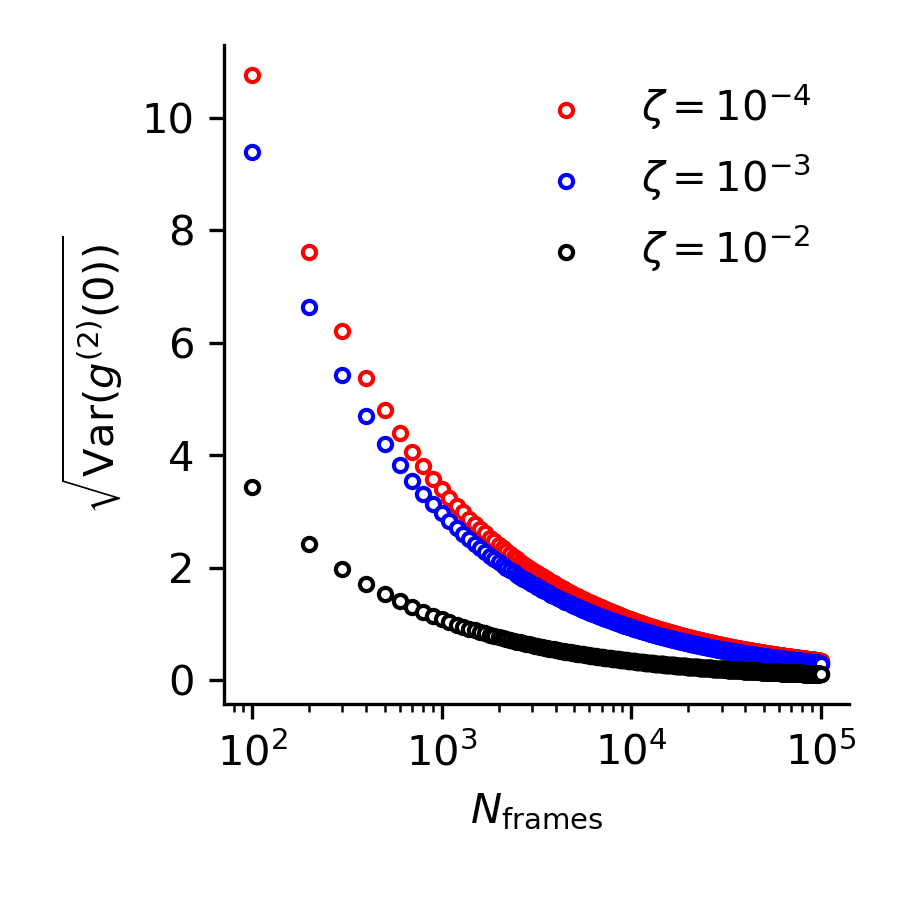
\includegraphics[width=8cm]{/Users/cwseitz/git/cwseitz.github.io/docs/phd/spad/spad/media/g20g2m_3.png}
%\caption{\textbf{Error in the second-order coherence dip}. Precision of the $g^{(2)}(0)$ estimate depends on the number of total frames (total photons) collected in the sequence. }
%\label{fig:atto}
%\end{figure}  



%\begin{figure*}[t]
%\centering
%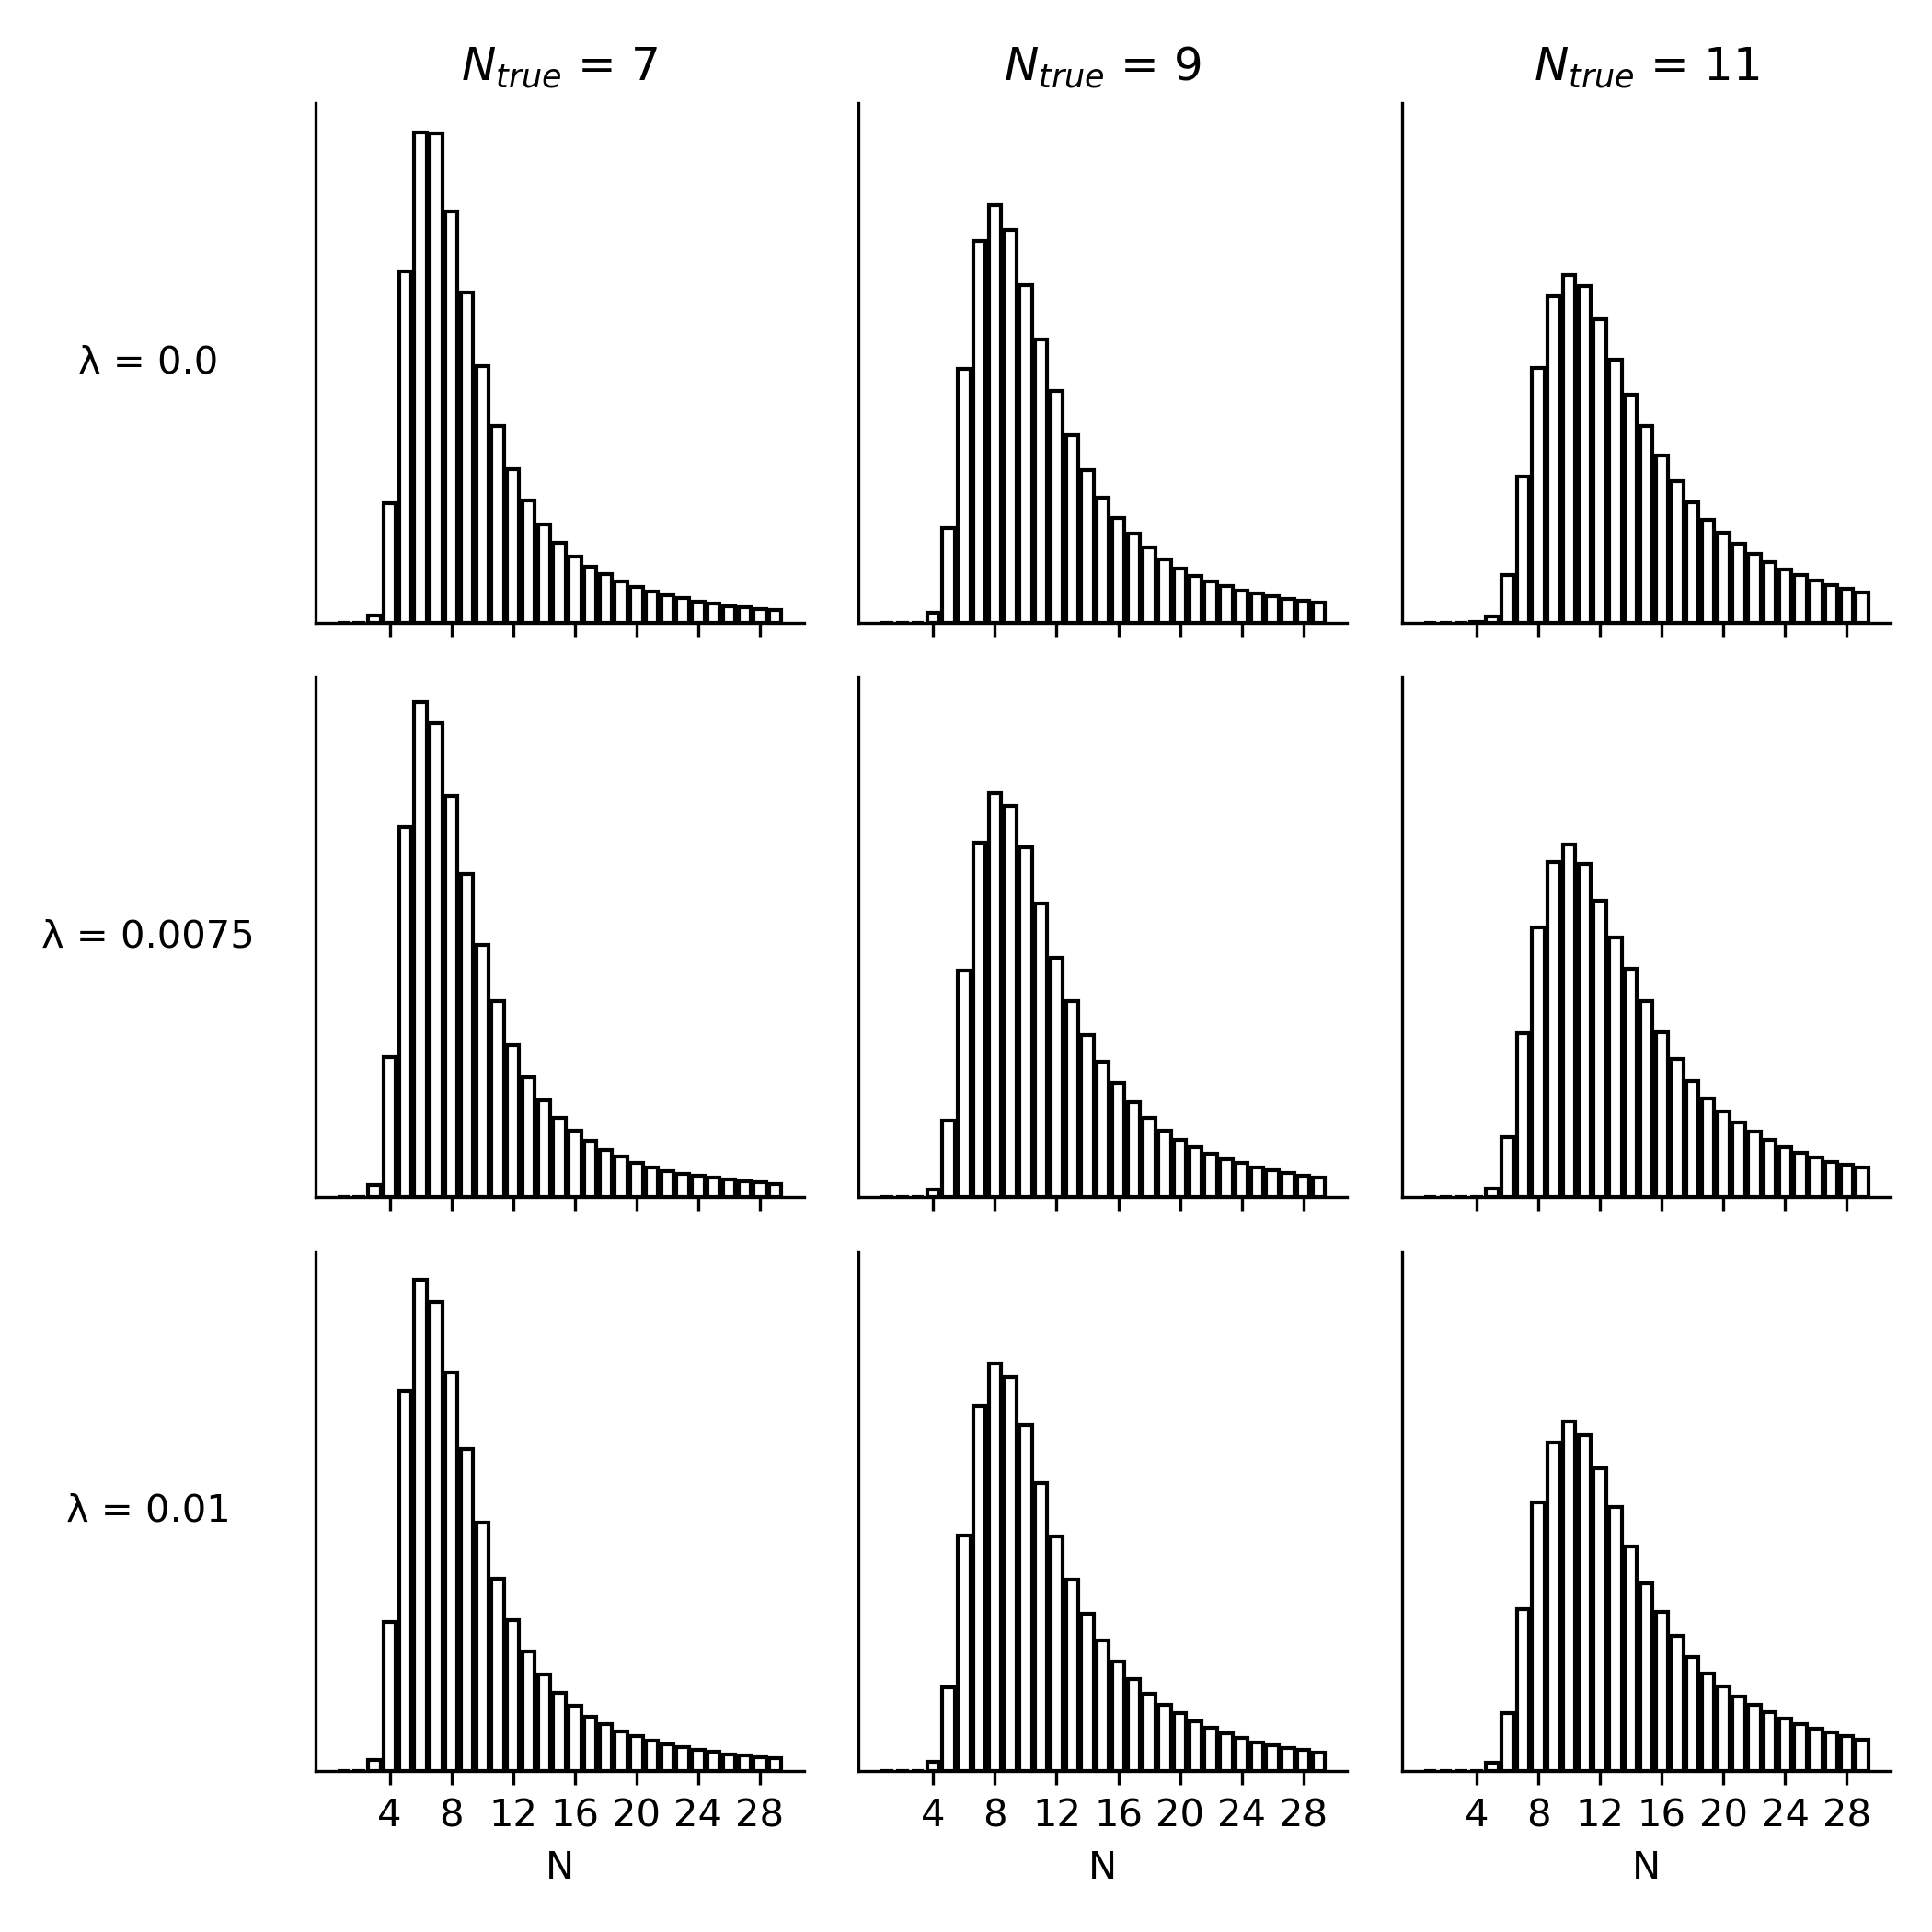
\includegraphics[width=14cm]{/Users/cwseitz/git/cwseitz.github.io/docs/phd/spad/spad/media/PoissonBinomialPost-2.png}
%\caption{\textbf{Posterior distributions of the fluorophore number}. Samples from the Poisson-Binomial convolution distribution using $\zeta=0.01$ for various values of $\lambda$ and $N=7,9,11$ were simulated. The variable $\zeta$ was integrated out by Monte Carlo integration, sampling 1000 $\zeta$ values from the posterior distribution (see main text for details)}
%\label{fig:fig10}
%\end{figure*}    

%\begin{figure*}[t]
%\centering
%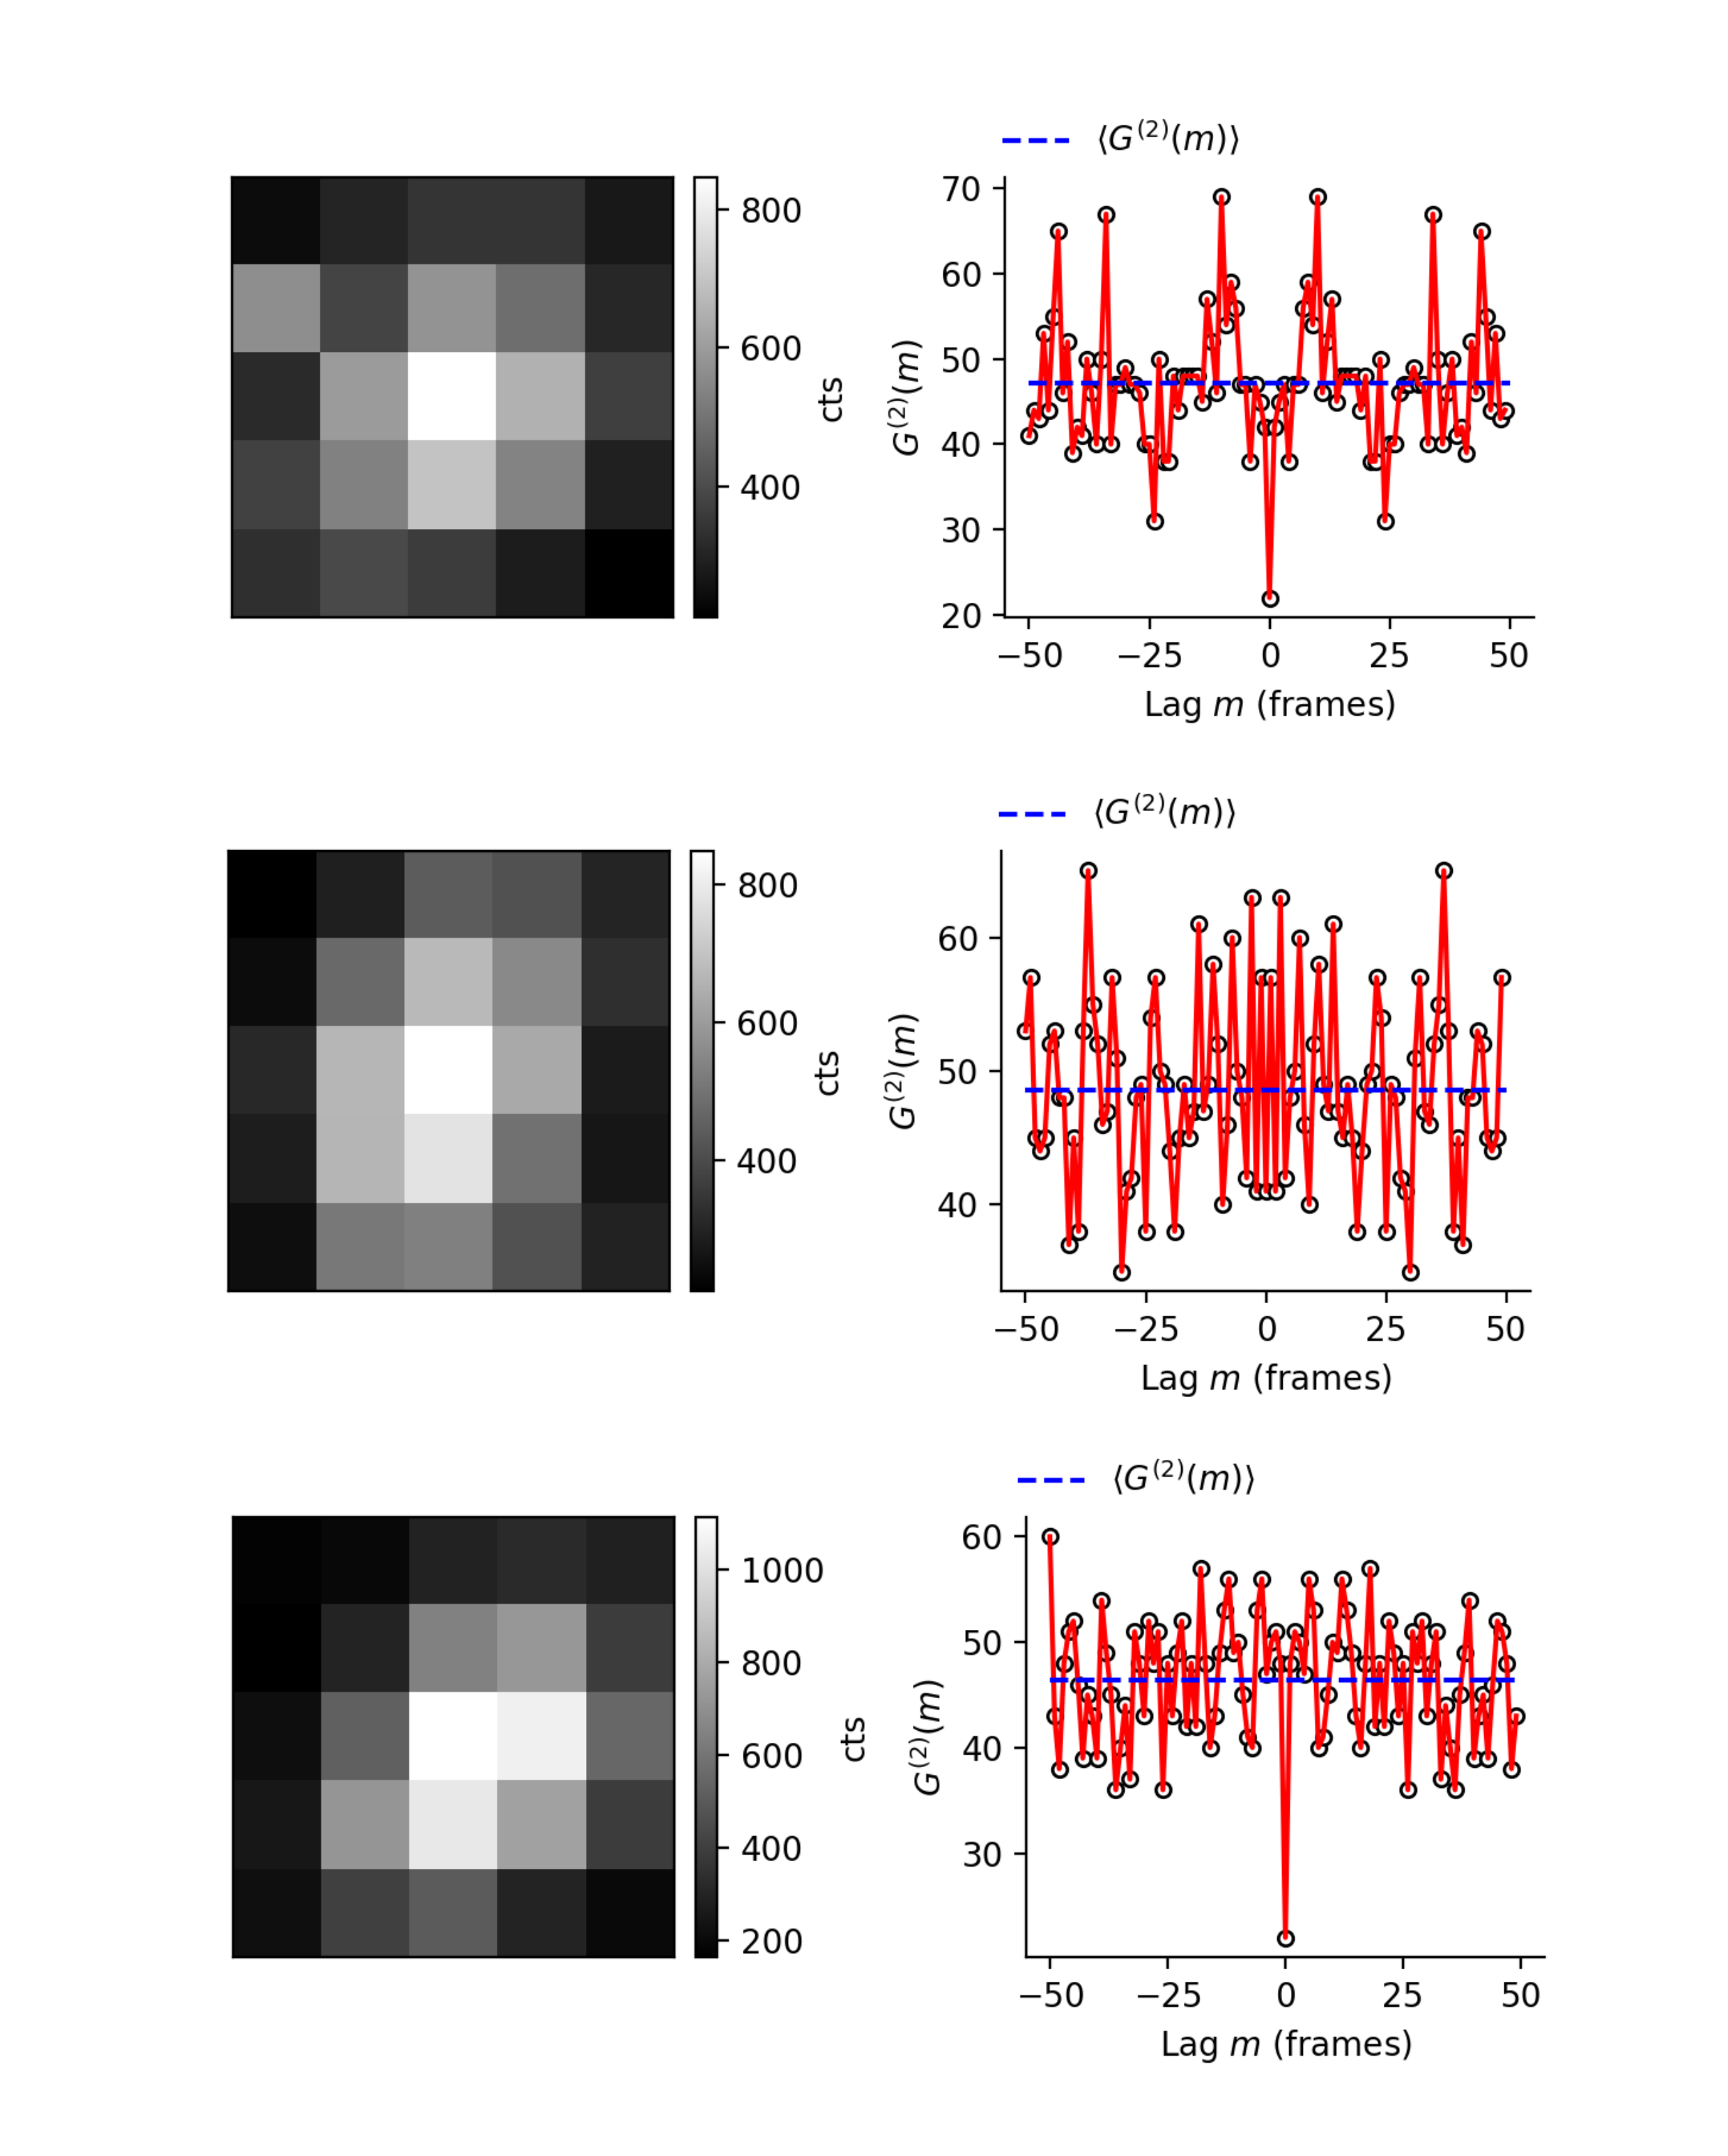
\includegraphics[width=14cm]{/Users/cwseitz/git/cwseitz.github.io/docs/phd/spad/spad/media/G2.png}
%\caption{\textbf{Example $G^{(2)}(m)$ functions}. Example quantum dot images and respective $G^{(2)}(m)$ functions, taken with 1us frames 500kHz laser repetition rate.}
%\label{fig:fig32}
%\end{figure*}    

\subsection{Discussion}

%Fluorescence intermittency can affect the observed photon-number fluctuations and could be expected to affect the value of $g^{(2)}(0)$ or the posterior on the number of active fluorescent emitters. However, the signal photon number per frame will follow Binomial statistics even in the presence of blinking, the only consequence of which is an effective reduction of the detection probability $\zeta$. If the effect of censoring photons by blinking and lowering the quantum yield can be accounted for, the technique used here may be compatible with common super-resolution techniques such as stochastic optical reconstruction microscopy (STORM). 

%The acquisition times necessary to obtain sufficient photon counts for computing the necessary statistics can potentially be very short. Most fluorophores have relaxation times in the nanosecond range and thus photons can be collected at a rate of at tens of millions of excitation pulses per second. These rates are currently difficult to obtain, however, due to limitations in triggering frequency and detector throughput. The SPAD camera used in this study has a minimum exposure time of 20 nanoseconds. Furthermore, the data volume can quickly become intractable due to the need for several thousands of frames for a millisecond-scale exposure time. This is currently a complication for techniques like STORM and advancements in the automation for data acquisitions are necessary. The speed of MCMC based localization remains a limitation for post-processing, and optimization of the processing time for localization is left for future work. 

%In conclusion, we propose a single molecule imaging technique that allows for counting of fluorescent molecules by modeling the quantum properties of fluorescence emission. The technique does not require a nonclassical light source and is designed to supplement standard single molecule localization microscopy techniques. The proposed method can be implemented with a standard widefield fluorescence microscope.

Here, we leveraged the recently developed SPAD array to spatially resolve the photon counting histogram with a widefield microscope. The PCH was integrated into a Bayesian inference scheme to extract the number of fluorescent emitters throughout the field of view and measure the second order coherence function. We demonstrated accurate counting of fluorescent quantum dots and fluorescent dyes bound to DNA origami, suggesting that this is a capable method for quantitative widefield fluorescent microscopy. Future work may assess more complex fluorescent imaging scenarios. 

For example, fluorescence intermittency or photobleaching leads to a $\zeta(t)$ which is not constant and can be fluorophore specific. This may affect the observed photon-number fluctuations and the PCH function $\mathcal{L}_{signal}(n_{\mathrm{signal}})$ used here may no longer be stationary. Therefore, due to the unique dynamics of $\zeta(t)$ for each fluorophore, the use of (2) is no longer appropriate and one can expect more complex behavior of $g^{(2)}(0)$. As an example, challenges may arise in distinguishing one homogeneously emitting fluorophore and several blinking fluorophores. If the effect of censoring photons by blinking can be accounted for, the technique used here may be compatible with common nanoscopy methods which rely on fluorescence intermittency. However, neither of these effects need be considered here. The tested quantum dots are photostable and photobleaching of ATTO532 could be mitigated under the experimental conditions used. Moreover, the on and off state lifetime of tested quantum dots and are significantly longer than the acquisition sequence, making fluorescence intermittency negligible. 
 
The acquisition times necessary to obtain sufficient photon counts for computing the necessary statistics can potentially be very short. Most fluorophores have relaxation times in the nanosecond range and thus photons can be collected at a rate of tens of millions of excitation pulses per second. These rates are currently difficult to obtain, however, due to limitations in detector throughput. Moreover, the data volume can quickly become intractable due to the need for several thousands of frames for a millisecond-scale exposure time. 

Theoretical and experimental estimation of $g^{(2)}(0)$ demonstrate that the suitability of this measure can depend on experimental conditions. Collection of thousands of photons is necessary to reduce the error in the $g^{(2)}(0)$ value to its minimal value. Furthermore, we showed experimentally that low signal to background ratios results in loss of the binomial character of the data. This suggests the compatibility of bright fluorophores (such as quantum dots) for antibunching-based measurements. On the other hand, the Bayesian inference scheme of the fluorophore number will not be as sensitive to the fluorophore brightness in this way, as the PCH can effectively model various $\zeta$ values. 

Lastly, the method proposed here may lead to significant advances in localization microscopy. Many of these schemes utilize the concept of precise localization of fluorescent emitters to produce super-resolved images \parencite{Rust2006,Betzig2006}. However, an inherent problem with such methods is the assumption that fluorescent emitters are isolated, which can lead to undercounting and localization errors. Various models for multi-emitter localization have been developed to approach this issue statistically \parencite{Nehme2020,Speiser2021,Li2019,Fazel2019}, which necessarily treat the number of fluorescent emitters as an unknown. The approach proposed here provides a physical means to quantifying active fluorescent emitters based on widefield photon counting.

In conclusion, we propose a single molecule imaging technique that allows for counting of fluorescent molecules by modeling the quantum properties of fluorescence emission. The technique does not require a nonclassical light source and is designed to supplement standard single molecule localization microscopy techniques. The proposed method can be implemented with a standard widefield fluorescence microscope.

\clearpage
\begin{figure}
\centering
\includegraphics[width=16cm]{/Users/cwseitz/git/cwseitz.github.io/docs/phd/spad/spad/media/Figure-2.png}
\caption{\textbf{Theoretical scaling of the second-order coherence with the fluorophore number}. (a) Expected number of coincidences at zero-lag (black) and the $g^{(2)}(0)$ ratio (red) in the case of pure binomial or pure Poisson photon statistics, as a function of the fluorophore number. Poisson and Binomial data are assumed to have an identical mean of 0.01 (b) $g^{(2)}(0)$ as a function of the fluorophore number for zero background conditions (pure binomial statistics) and various $\zeta$ values. (c) $g^{(2)}(0)$ as a function of the fluorophore number for nonzero background conditions (Poisson-Binomial statistics, $\lambda=0.0075$) and various $\zeta$ values.}
\label{fig:binomvpoiss}
\end{figure}  


\begin{figure*}
\centering
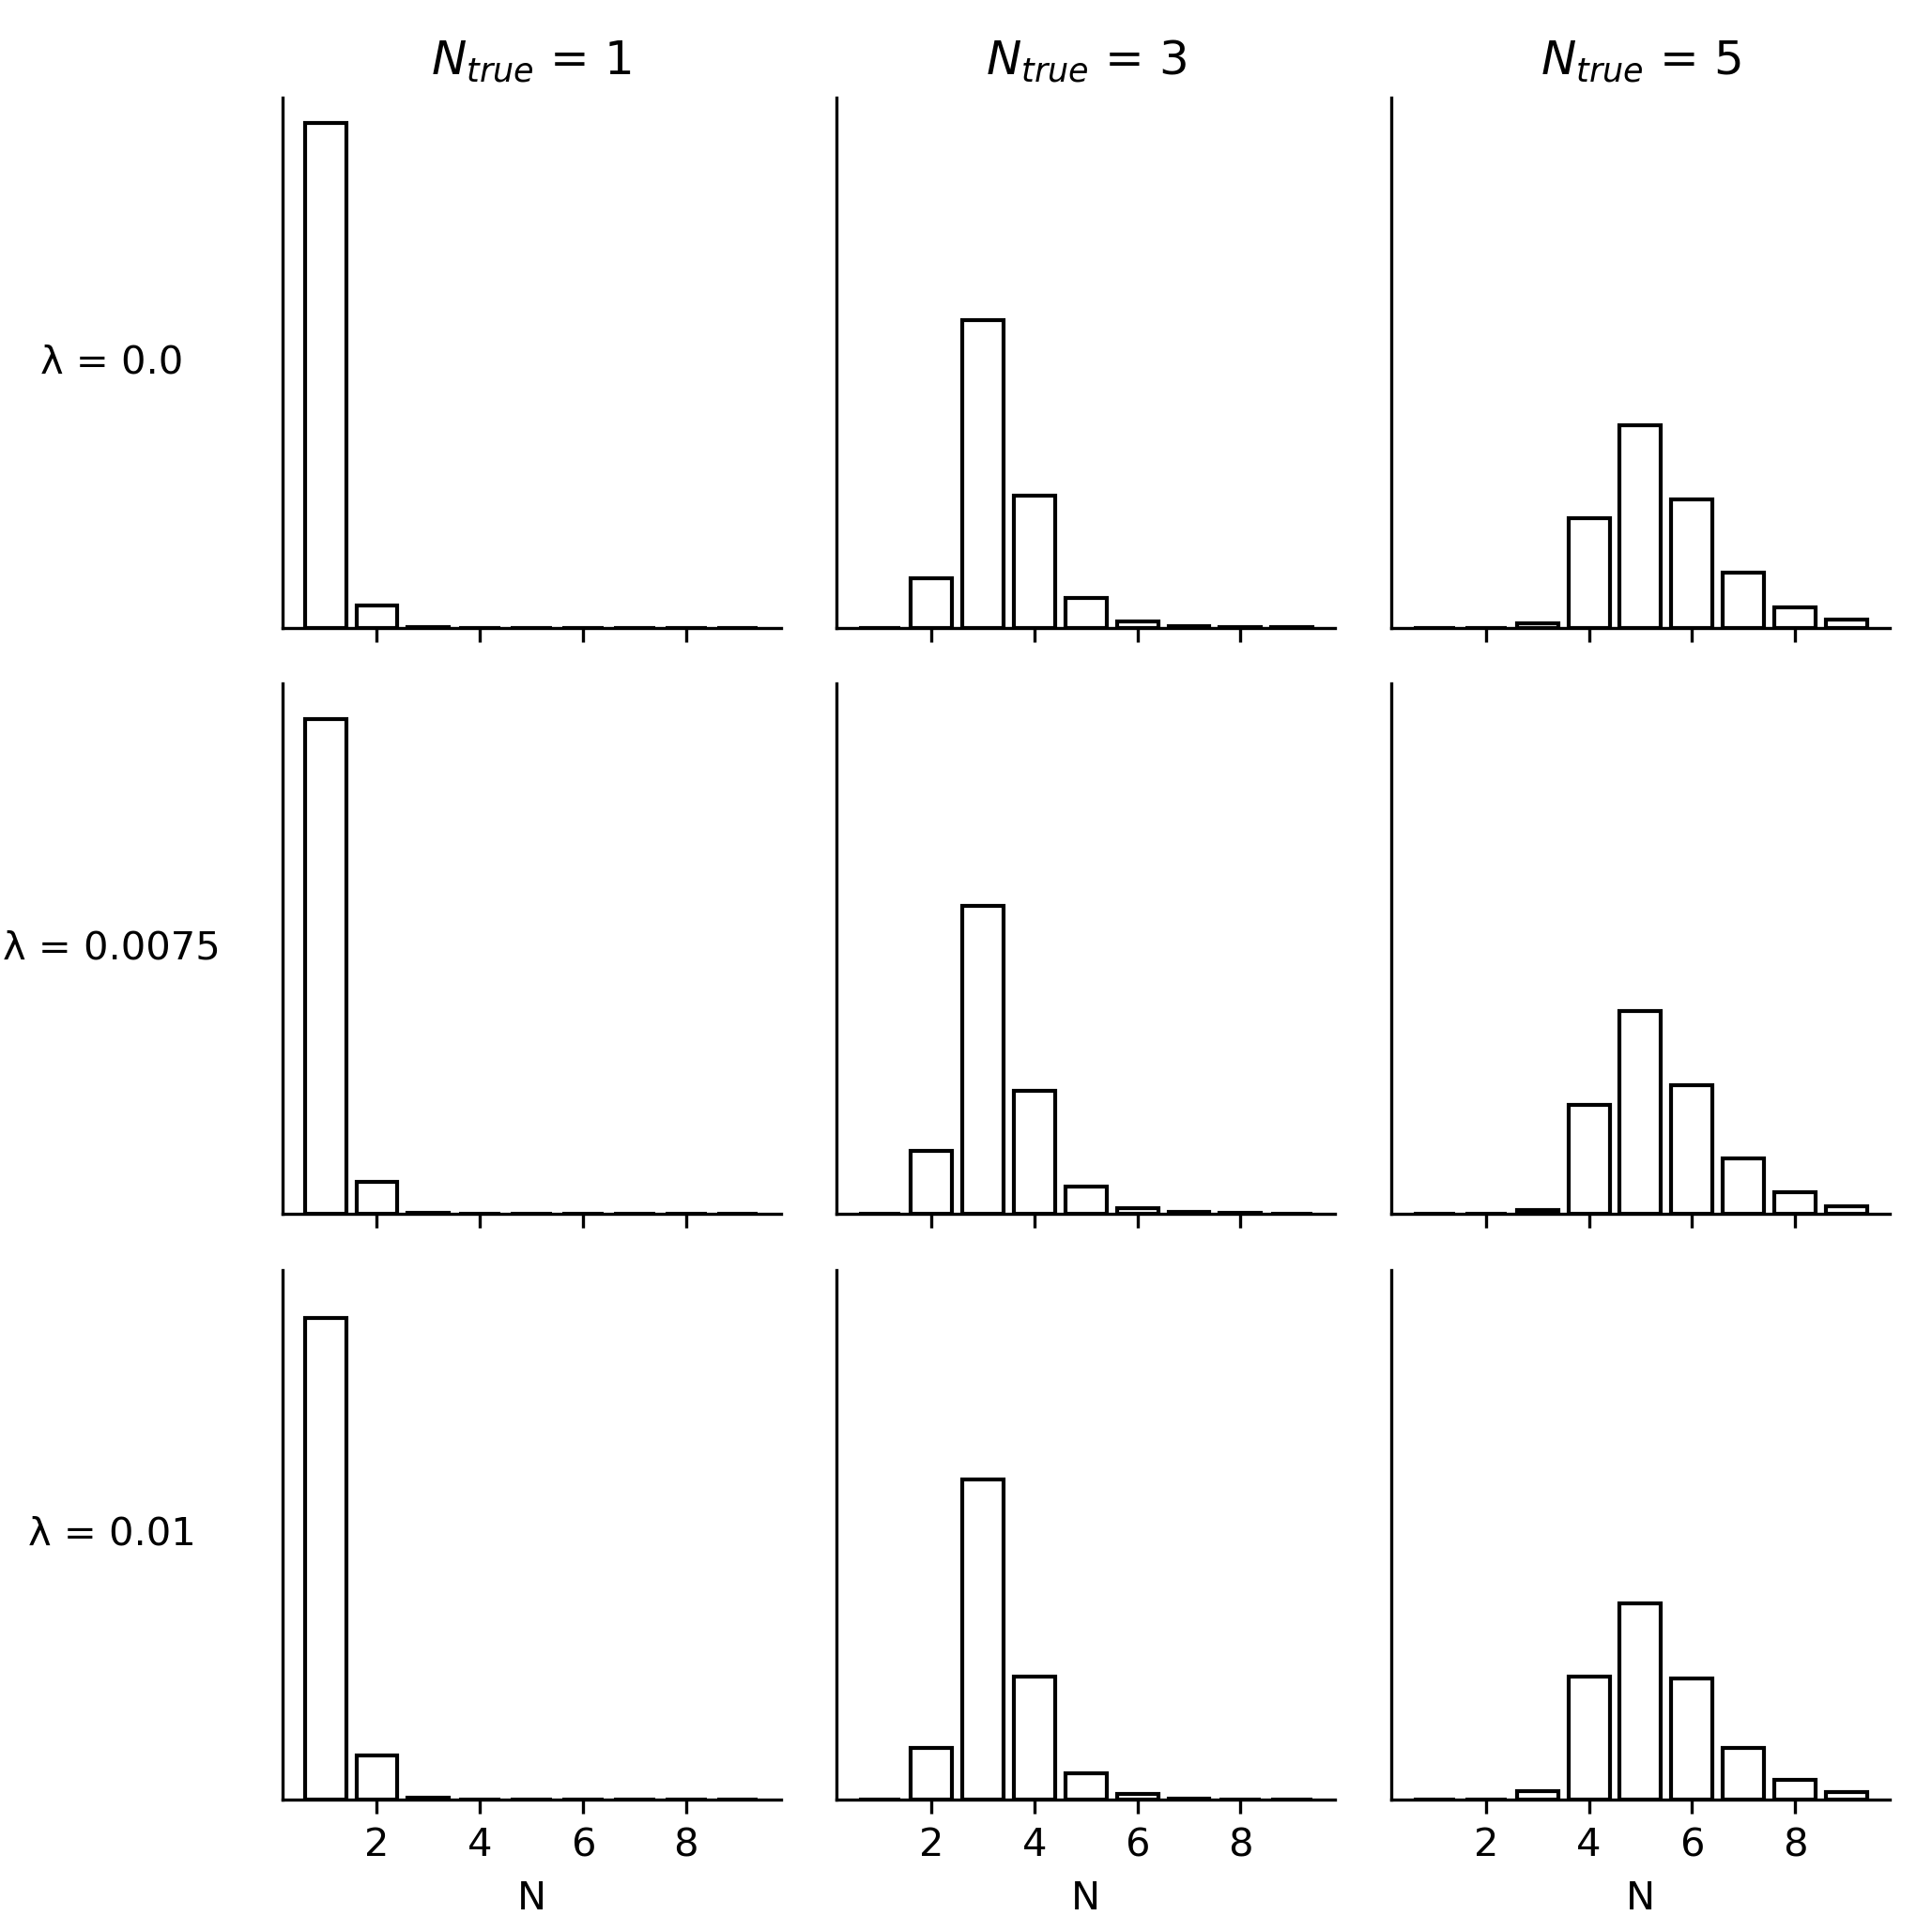
\includegraphics[width=14cm]{/Users/cwseitz/git/cwseitz.github.io/docs/phd/spad/spad/media/PoissonBinomialPost-1.png}
\caption{\textbf{Posterior distributions of the fluorophore number}. Samples from the Poisson-Binomial convolution distribution using $\zeta=0.01$ for various values of $\lambda$ and $N=1,3,5$ were simulated. The variable $\zeta$ was integrated out by Monte Carlo integration, sampling 1000 $\zeta$ values from the posterior distribution (see main text for details)}
\label{fig:fig9}
\end{figure*}    

\clearpage
\section{Future directions: quantum illumination strategies}

In recent years, novel quantum illumination strategies have leveraged spatial correlations between downconverted photon pairs to demonstrate the first quantum illumination full-field imaging protocol. These spatial quantum correlations are generated by a nonlinear optical process referred to as spontaneous parametric downconversion (SPDC). SPDC is typically realized using a nonlinear crystal such as Beta Barium Borate (BBO) or $\beta$-BaB$_2$O$_4$. BBO crystals are highly anisotropic and exhibit nonlinear optical properties, which means that polarization of the crystal varies nonlinearly with electric field strength. This nonlinear behavior can lead to a number of useful effects such as second harmonic generation, third harmonic generation, or SPDC \parencite{Boyd2020}. In the SPDC process, a pump photon typically in the ultraviolet range is downconverted into a pair of lower-energy photons, with wavelengths in the visible range. These photons are known as signal and idler photons. This process is a purely quantum mechanical one, and the daughter photons born in this process possess useful quantum mechanical properties. Indeed, physical principles such as conservation of energy and momentum require that the daughter photons born in this nonlinear process are spatially entangled in several degrees of freedom \parencite{Boyd2020}. 


A relatively straightforward application of SPDC is prediction of photon arrival times of the signal beam by measurement of the idler beam with a single photon sensitive detector. For example, this has been applied to improve the signal-to-noise ratio for measuring the absorption of objects through sub–shot-noise measurements \parencite{Brida2010} or imaging through detector noise and background signal \parencite{Gregory2020,Wolley2022}. In such applications, twin beams produced through the SPDC process are directed to different regions of a spatially resolved detector such as a CCD camera or single-photon avalanche diode (SPAD) array detector. By performing a pixel-by-pixel AND-operation between two regions of the array detector containing the SPDC beams, we can preferentially select correlated photon-pair events and reject uncorrelated background light and sensor noise events. Heralding photons using the signal and idler beams involves detecting one photon (either the signal or idler) and using this detection to infer the presence of its entangled counterpart. This method enhances the precision of photon detection and significantly improves the signal-to-noise ratio in quantum imaging.

This methodology has yet to be fully demonstrated in single molecule imaging or localization microscopy, which is generally quite sensitive to background signal or detector noise. Moreover, typical CCD	 technologies do not possess the time resolution of novel SPAD arrays, which may permit spatially resolved coincidence detection of photon pairs with nanosecond time resolution. Incorporating this technique into fluorescence imaging may further enhance the imaging quality and localization precision. By utilizing the known fluorescence lifetime of a single photon source such as a fluorescent dye molecule, one can possibly herald a fluorescence photon by measurement of the idler beam.


\ProvidesFile{ch2.tex}[]

\chapter{UNCERTAINTY AWARE LOCALIZATION MICROSCOPY BY VARIATIONAL DIFFUSION}
\ix{physics//Physics appendix}

\section{Background}

\subsection{The curse of dimensionality}

Dimensionality refers to the number of variables or features in a dataset. In conventional fluorescence nanoscopy, an image generated by (1.1) containing $M$ fluorophores has $2M$ parameters. Similarly, the image itself is a high dimensional variable where the number of pixels is the number of dimensions. As the number of dimensions in the parameter space increases, it becomes increasingly difficult to infer the parameters from the data. The curse of dimensionality is a term coined to describe various phenomena that arise when working with high-dimensional data, making statistical analysis and machine learning more challenging. Mathematically, the curse of dimensionality can be described through the following issues.

As dimensionality increases, the volume of the space grows exponentially. For instance, the volume of a hypercube with side length $l$ in $d$-dimensional space is given by $l^d$. This rapid increase in volume means that data points become sparser, making it difficult to estimate densities and find meaningful patterns. Furthermore, in high-dimensional spaces, the concept of distance becomes less informative. The difference between the minimum and maximum distance between data points tends to shrink as dimensionality increases, which can make clustering and nearest-neighbor algorithms less effective. With a large number of dimensions, models can easily become overly complex, capturing noise instead of the underlying signal. This leads to overfitting, where the model performs well on training data but poorly on unseen data.

Deep models have captured the attention of many researchers, as they can perform inference tasks in high dimensional spaces without an excessive computational burden. These models are not entirely immune to the curse of dimensionality or the complexity of data distributions, however, and overfitting is still an important problem. Simultaneously, many deep models are deterministic neural networks, which give a single output given an input. This is in sharp contrast to classical statistical inference methodologies such as Bayesian inference, which model a distribution on their outputs, allowing one to express uncertainties during inference. Bayesian methods such as Markov Chain Monte Carlo (MCMC) or variational inference lack the scaling of deep learning but maintain a scientific value \parencite{Kingma2013}.

\subsection{The Bayesian calculation}

Bayesian inference provides a rigorous framework for updating beliefs about the world in light of new data. It leverages the principles of probability theory to combine prior knowledge with empirical evidence, resulting in updated, posterior beliefs. In parametric modeling, we assume that the data $x$ are generated from a distribution with a set of parameters $y$. Parametric models simplify the problem by assuming a specific form for the underlying distribution of the data, characterized by a finite set of parameters. This approach allows us to use mathematical functions to describe complex systems and make inferences about the parameters based on observed data.

At the heart of Bayesian inference is Bayes' rule, which allows us to update our beliefs based on new evidence. Bayes' rule is derived from the definition of conditional probability. The conditional probability of $y$ given $x$ is defined as $p(y \lvert x) = \frac{p(x,y)}{p(y)}$ provided that $p(y) > 0$. Similarly, the conditional probability of $x$ given $y$ is $p(x \lvert y) = \frac{p(x,y)}{p(x)}$. Rearranging these equations and solving for $p(y\lvert x)$ gives us Bayes' rule:

\begin{equation*}
p(y \lvert x) = \frac{p(x \lvert y) p(y)}{p(x)}.
\end{equation*}

Here, $p(y \lvert x)$ is the called the posterior distribution, representing our updated beliefs about the parameters after observing the data. $p(x \lvert y)$ is the likelihood, the probability of the observed data given the parameters. $p(y)$ is the prior distribution, representing our beliefs about the parameters before observing the data. $p(x)$ is the marginal likelihood or evidence, which normalizes the posterior distribution and ensures it sums to one.

One of the main challenges in Bayesian inference is the computation of the posterior distribution. The denominator in Bayes' rule, $p(x)$, involves an integral over all possible values of the parameters:

\begin{equation*}
p(x) = \int p(x \lvert y) p(y) \, dy.
\end{equation*}

In many practical applications, this integral is intractable due to the high dimensionality of the parameter space. To address this challenge, various approximation methods have been developed. One such method is Markov Chain Monte Carlo (MCMC), which generates samples from the posterior distribution by constructing a Markov chain that has the desired distribution as its equilibrium distribution. MCMC algorithms were originally developed for applications in statistical physics but were eventually adapted to a broader range of statistical problems. Well known MCMC algorithms include the Metropolis-Hastings algoritm, Gibbs sampler \parencite{Geman1984}, and gradient-based algorithms inspired by Langevin dynamics. In general, MCMC is asymptotically exact but can be computationally expensive for large datasets and high dimensional parameter spaces. Variational inference is an alternative approach, which is not exact, but reduces the computational burden in these scenarios.

\subsection{Variational inference}

Variational inference involves approximating the true posterior distribution \( q(y \lvert x) \) with a simpler, parameterized distribution \( p_{\psi}(y) \) by minimizing the Kullback-Leibler (KL) divergence between them. The KL divergence \( D_{KL}(q(y \lvert x) \lvert\lvert p_{\psi}(y)) \) measures how one probability distribution diverges from a second probability distribution. To minimize the KL divergence, we first express it as

\begin{equation}
D_{KL}(q(y \lvert x) \lvert\lvert p_{\psi}(y)) = \mathbb{E}_{q(y \lvert x)}\left[\log \frac{q(y \lvert x)}{p_{\psi}(y)}\right]
\end{equation}

This can be rewritten using Bayes' rule as

\begin{align*}
D_{KL}(q(y \lvert x) \lvert\lvert p_{\psi}(y\lvert x)) &= \mathbb{E}_{q(y \lvert x)}\left[\log \frac{q(y \lvert x)}{p_{\psi}(y\lvert x)}\right] \\
&= \mathbb{E}_{q(y \lvert x)}\left[\log \frac{q(y\lvert x)p_{\psi}(x)}{p_{\psi}(x,y)} \right]\\
&= \mathbb{E}_{q(y \lvert x)}\left[\log \frac{q(y\lvert x)}{p_{\psi}(x,y)} \right] + \mathbb{E}_{q(y \lvert x)}\left[\log p_{\psi}(x) \right]
\end{align*}

Defining $\mathcal{L} = -\mathbb{E}_{q(y \lvert x)}\left[\log \frac{q(y\lvert x)}{p_{\psi}(x,y)} \right]  = \mathbb{E}_{q(y \lvert x)}\left[\log \frac{p_{\psi}(x,y)}{q(y\lvert x)} \right] $, we can write,

\begin{equation}
\mathbb{E}_{q(y \lvert x)}\left[\log p_{\psi}(x) \right] = D_{KL}(q(y \lvert x) \lvert\lvert p_{\psi}(y\lvert x)) + \mathcal{L} \geq \mathcal{L}
\end{equation}

which is often called a variational objective. Given that \( \log p_{\psi}(x) \) is constant, minimizing $D_{KL}(q(y \lvert x) \lvert\lvert p_{\psi}(y\lvert x))$ is equivalent to maximizing $\mathcal{L}$. For practical reasons, we often instead solve a minimization problem with respect to $\psi$

\begin{equation}
\mathbb{E}_{q(y \lvert x)}\left[-\log p_{\psi}(x) \right] \leq -\mathcal{L} = \mathbb{E}_{q(y \lvert x)}\left[-\log \frac{p_{\psi}(x,y)}{q(y\lvert x)} \right]
\end{equation}

This approach provides a practical way to perform Bayesian inference, especially in high-dimensional settings. It is worth noting that this derivation often begins by taking the expectation with respect to the model distribution, since the true distribution is unknown. However, for the following application, the target distribution is known and thus the objective is formulated in this way. 


%\subsection{A note on variational inference for functions}

%For some applications, we would like to perform inference when the mapping between latents and observed data is deterministic. For example, there might be a determinisitic mapping $f$ between high resolution images and low-resolution ones, and we want to infer the high resolution image from the low resolution image. In that case, we find

%\begin{align*}
%\mathbb{E}_{q(y \lvert x)}\left[-\log p_{\psi}(x) \right] &\leq \mathbb{E}_{q(y \lvert x)}\left[-%\log \frac{p_{\psi}(x,y)}{q(y\lvert x)} \right]\\
%&= \mathbb{E}_{q(y \lvert x)}\left[-\log \frac{p_{\psi}(y)}{q(y\lvert x)} \right] + \mathbb{E}_{q(y \lvert x)}\left[-\log p_{\psi}(x\lvert y) \right] \\
%&= \mathbb{E}_{q(y \lvert x)}\left[-\log \frac{p_{\psi}(y)}{q(y\lvert x)} \right] + \mathbb{E}_{q(y \lvert x)}\left[-\log \delta(x-f(y)) \right] 
%\end{align*}

%The second term is to be safely neglected, as it is undefined and provides no meaningful information during optimization. 

\section{Uncertainty-aware localization microscopy}

Deep models have attracted tremendous attention from researchers in the natural sciences, with several foundational applications arising in microscopy \parencite{Weigert2018,Falk2019}. In particular, the application of deep models for image restoration in single-molecule localization microscopy (SMLM) has received considerable interest. The use of deep models in localization microscopy has been proposed as an alternative to traditional localization algorithms to increase imaging speed and enhance spatial resolution. For example, localization in dense scenes has been performed using traditional convolutional networks to reduce the total acquisition time to generate a super-resolution image \parencite{Nehme2020,Speiser2021}.

Localization in dense scenes is a difficult inverse problem, and a single measurement can underdetermine the number of spots and their respective locations. Since this problem is ill-posed, we choose to model the uncertainty directly. Therefore, we approach localization in dense scenes by predicting high-resolution kernel density (KD) estimates from low resolution images using a diffusion model. Diffusion models can model the conditional probability distribution on high-resolution images given low-resolution inputs. This contrasts with traditional methods based on convolutional networks, which provide point estimates and preclude computation of uncertainty at test time under a fixed model. 

Our implementation is based on the conditional variational diffusion model (CVDM) – a type of continuous-time diffusion model developed in the context of image super-resolution \parencite{Maggiora2023}. CVDM is inspired by recent variational perspectives on diffusion \parencite{Dirmeier2023,Ribeiro2024,Kingma2021,Kingma2023}. Variational diffusion models provide a mechanism for scalable inference, which can be trained using a variational bound written in terms of the signal-to-noise ratio of the diffused data, and a simple noise estimation loss. In the remainder of this paper, we introduce a generative model on dense localization microscopy images and use it to simulate data for training and validation of CVDM. The model is then tested on experimental images of the nuclear pore complex protein 96 (Nup96) tagged with mMaple. 

\subsection{Approach}

\begin{figure}[t]
\centering
\includegraphics[scale=0.6]{/Users/cwseitz/git/cwseitz.github.io/docs/phd/ddpm/ddpm/media/Figure-0.png}
\caption{Generative model of single molecule localization microscopy images. Low resolution images $\bold{x}$ are generated from coordinates $\theta$ by integration of the optical transfer function $O$ and sampling from the likelihood (1): $\bold{x}\sim p(\bold{x}\lvert\theta) = \prod_{k} p(\bold{x}_k\lvert\theta)$. A kernel density estimate $\bold{y}$ is inferred from $\bold{x}$}
\label{fig:fig60}
\end{figure}


Direct optimization of the image likelihood from observations $\bold{x}$ alone is challenging when fluorescent emitters are dense within the field of view and fluorescent signals significantly overlap. However, CNNs have recently proven to be powerful tools fluorescence microscopy to extract parameters describing fluorescent emitters such as color, emitter orientation, $z$-coordinate, and background signal \cite{Zhang2018,Kim2019,Zelger2018}. For localization tasks, CNNs typically employ upsampling layers to reconstruct Bernoulli probabilities of emitter occupancy \parencite{Speiser2021,Nehme2020}. We choose to instead infer KDEs, denoted by $\bold{y}$, which are latent in the low-resolution data $\bold{x}$. KDEs are a common data structure used in nanoscopy, and can be easily generated from molecular coordinates, alongside observations $\bold{x}$.

To go beyond point estimation of the KDE given the low-resolution data, we seek a generative model for the posterior. Unfortunately, the posterior can be intractable, since molecules cannot be easily resolved and therefore its dimensionality is not well-defined. To address this issue, we instead model a conditional distribution on the latent $\bold{y}$: $p(\bold{y}\lvert\bold{x})$, where $\bold{y}$ is of known dimensionality. We choose to model $p(\bold{y}\lvert\bold{x})$ with a diffusion model, given that the distribution $p(\bold{y}\lvert\bold{x})$ is expensive to compute.

%Sampling from diffusion models can be computationally expensive, given that generation amounts to solving a complex stochastic differential equation, effectively mapping a simple base distribution to the complex data distribution. The solution of such equations requires numerical integration with very small step sizes, resulting in thousands of neural network evaluations \parencite{Saharia2021,Vahdat2021}. For conditional generation tasks in high-risk applications, generation complexity is further exacerbated by the need for the highest level of detail in generated samples. Therefore, we propose that sampling is preceded by an augmentation network $\phi$, which in essence generates an initial estimate to guide the diffusion process. Reasoning for this choice in our application is two-fold:

%\textbf{Synthesis Speed}. By training the augmentation network $\phi$ to obtain an approximate estimate of the KDE, we can reduce the number of iterations, since the diffusion model only needs to model the remaining mismatch, resulting in a less complex model from which sampling becomes easier. Speed is critical in SMLM applications, which can produce thousands of images in a single experiment.

%\textbf{Sample Fidelity}. Since diffusion will often be initialized in low-density regions of the data distribution, inaccurate score estimation in these regions will negatively affect the sampling process. Moreover, mixing can be difficult because of the need of traversing low density regions to transition between modes of the distribution \parencite{Song2019}.

\subsection{Variational diffusion}

Diffusion models \parencite{Ho2020,Song2021} are a class of generative models originally inspired by nonequilibrium statistical physics, which slowly destroy structure in a data distribution via a fixed Markov chain referred to as the \emph{forward process}, which is characterized by a variance schedule $\gamma(t,\bold{x})$:

\begin{equation*}
q(\bold{y}(t)\lvert\bold{y}_{0}) = \mathcal{N}(\sqrt{\gamma(t,\bold{x})}\bold{y}_{0},(1-\gamma(t,\bold{x}))I)
\end{equation*}

which uses the variance-preserving conditions defined in previous models. Note that the continuous-time variance schedule $\gamma(t,\bold{x})$ is analogous to the discrete-time product of variances used in discrete models \parencite{Ho2020}. However, the relationship between the variance schedule $\gamma(t,\bold{x})$ and the variance between fixed time points is more complex in the continuous-time formalism. Following \parencite{Maggiora2023}, we define

\begin{equation*}
q(\bold{y}(t+\Delta t)\lvert\bold{y}(t)) = \mathcal{N}(\sqrt{1-\beta(t,\bold{x})}\bold{y}_{0},\beta(t,\bold{x})I)
\end{equation*}

where $\beta(t,\bold{x}) = 1 - \frac{\gamma(t+\Delta t,\bold{x})}{\gamma(t,\bold{x})}$. The value of $\beta(t,\bold{x})$ controls the variance of the transition of $\bold{y}(t)$ over a period of time $\Delta t$. The reverse process reads:

\begin{equation*}
p\left(\mathbf{y}\left(t\right)\lvert\mathbf{y}\left(t+\Delta t\right)\right)=\mathcal{N}\left(\mathbf{\mu}_\psi\left(\mathbf{y}\left(t+\Delta t\right)\right),\gamma\left(t,\mathbf{x}\right)I\right),
\end{equation*}

where $\mathbf{\mu}_\psi\left(\mathbf{y}\left(t+\Delta t\right)\right)$ is the estimated expected value of the transition distribution by a neural network $\psi$. Notice that, by the definition of the forward process, $\mathbf{y}\left(t+\Delta t\right)\sim q\left(\mathbf{y}(t+\Delta t)\lvert\mathbf{y}_0\right)$ can be reparametrized as 

\begin{equation*}
\mathbf{y}\left(t+\Delta t\right)=\sqrt{\gamma\left(t+\Delta t,\mathbf{x}\right)}\mathbf{y}_\mathbf{0}+\sqrt{1-\gamma\left(t+\Delta t,\mathbf{x}\right)}\boldsymbol{\epsilon},
\end{equation*}

where $\boldsymbol{\epsilon}\sim\mathcal{N}\left(0,\mathbf{I}\right)$. We can estimate $\mathbf{y}_\mathbf{0}$ by rearranging this expression and estimating the noise $\hat{\boldsymbol{\epsilon}}$:

\begin{equation*}
{\hat{\mathbf{y}}}_\mathbf{0}=\frac{1}{\sqrt{\gamma\left(t+\Delta t,\mathbf{x}\right)}}\left(\mathbf{y}\left(t+\Delta t\right)-\sqrt{1-\gamma\left(t+\Delta t,\mathbf{x}\right)}\hat{\boldsymbol{\epsilon}}\right).
\end{equation*}

To sample from the reverse process, we can sample from the forward process starting at ${\hat{\mathbf{y}}}_\mathbf{0}$. We find that $\mathbf{\mu}_\psi\left(\mathbf{y}\left(t+\Delta t\right)\right)$ can be computed from the noise estimate:

\begin{equation*}
\mathbf{\mu}_\psi\left(\mathbf{y}\left(t+\Delta t\right)\right)=\frac{1}{\sqrt{\gamma\left(t+\Delta t,\mathbf{x}\right)}}\left(\mathbf{y}\left(t+\Delta t\right)-\sqrt{1-\gamma\left(t+\Delta t,\mathbf{x}\right)}\hat{\boldsymbol{\epsilon}}\right).
\end{equation*}


%\begin{equation}
%q(\bold{y}_{T}\lvert\bold{y}_{0}) = \prod_{t=1}^{T}q(\bold{y}_{t}\lvert\bold{y}_{t-1}) \;\;\; q(\bold{y}_{t}\lvert\bold{y}_{t-1}) = \mathcal{N}\left(\sqrt{1-\beta_{t}}\bold{y}_{t-1},\beta_t I\right)
%\end{equation}


%\begin{figure}
%\includegraphics[scale=0.5]{/Users/cwseitz/git/cwseitz.github.io/docs/phd/ddpm/ddpm/media/%Diffusion.png}
%\caption{\textbf{Uncertainty estimation by variational diffusion}. Example diffusion process of the %latent high resolution image $\bold{y}$ conditioned on the low resolution image $\bold{x}$. The %terminal $\bold{y}_{0}$ represents a sample from $p(\bold{y}\lvert\bold{x})$.}
%\label{fig:fig11}
%\end{figure}


\begin{figure}[t]
\centering
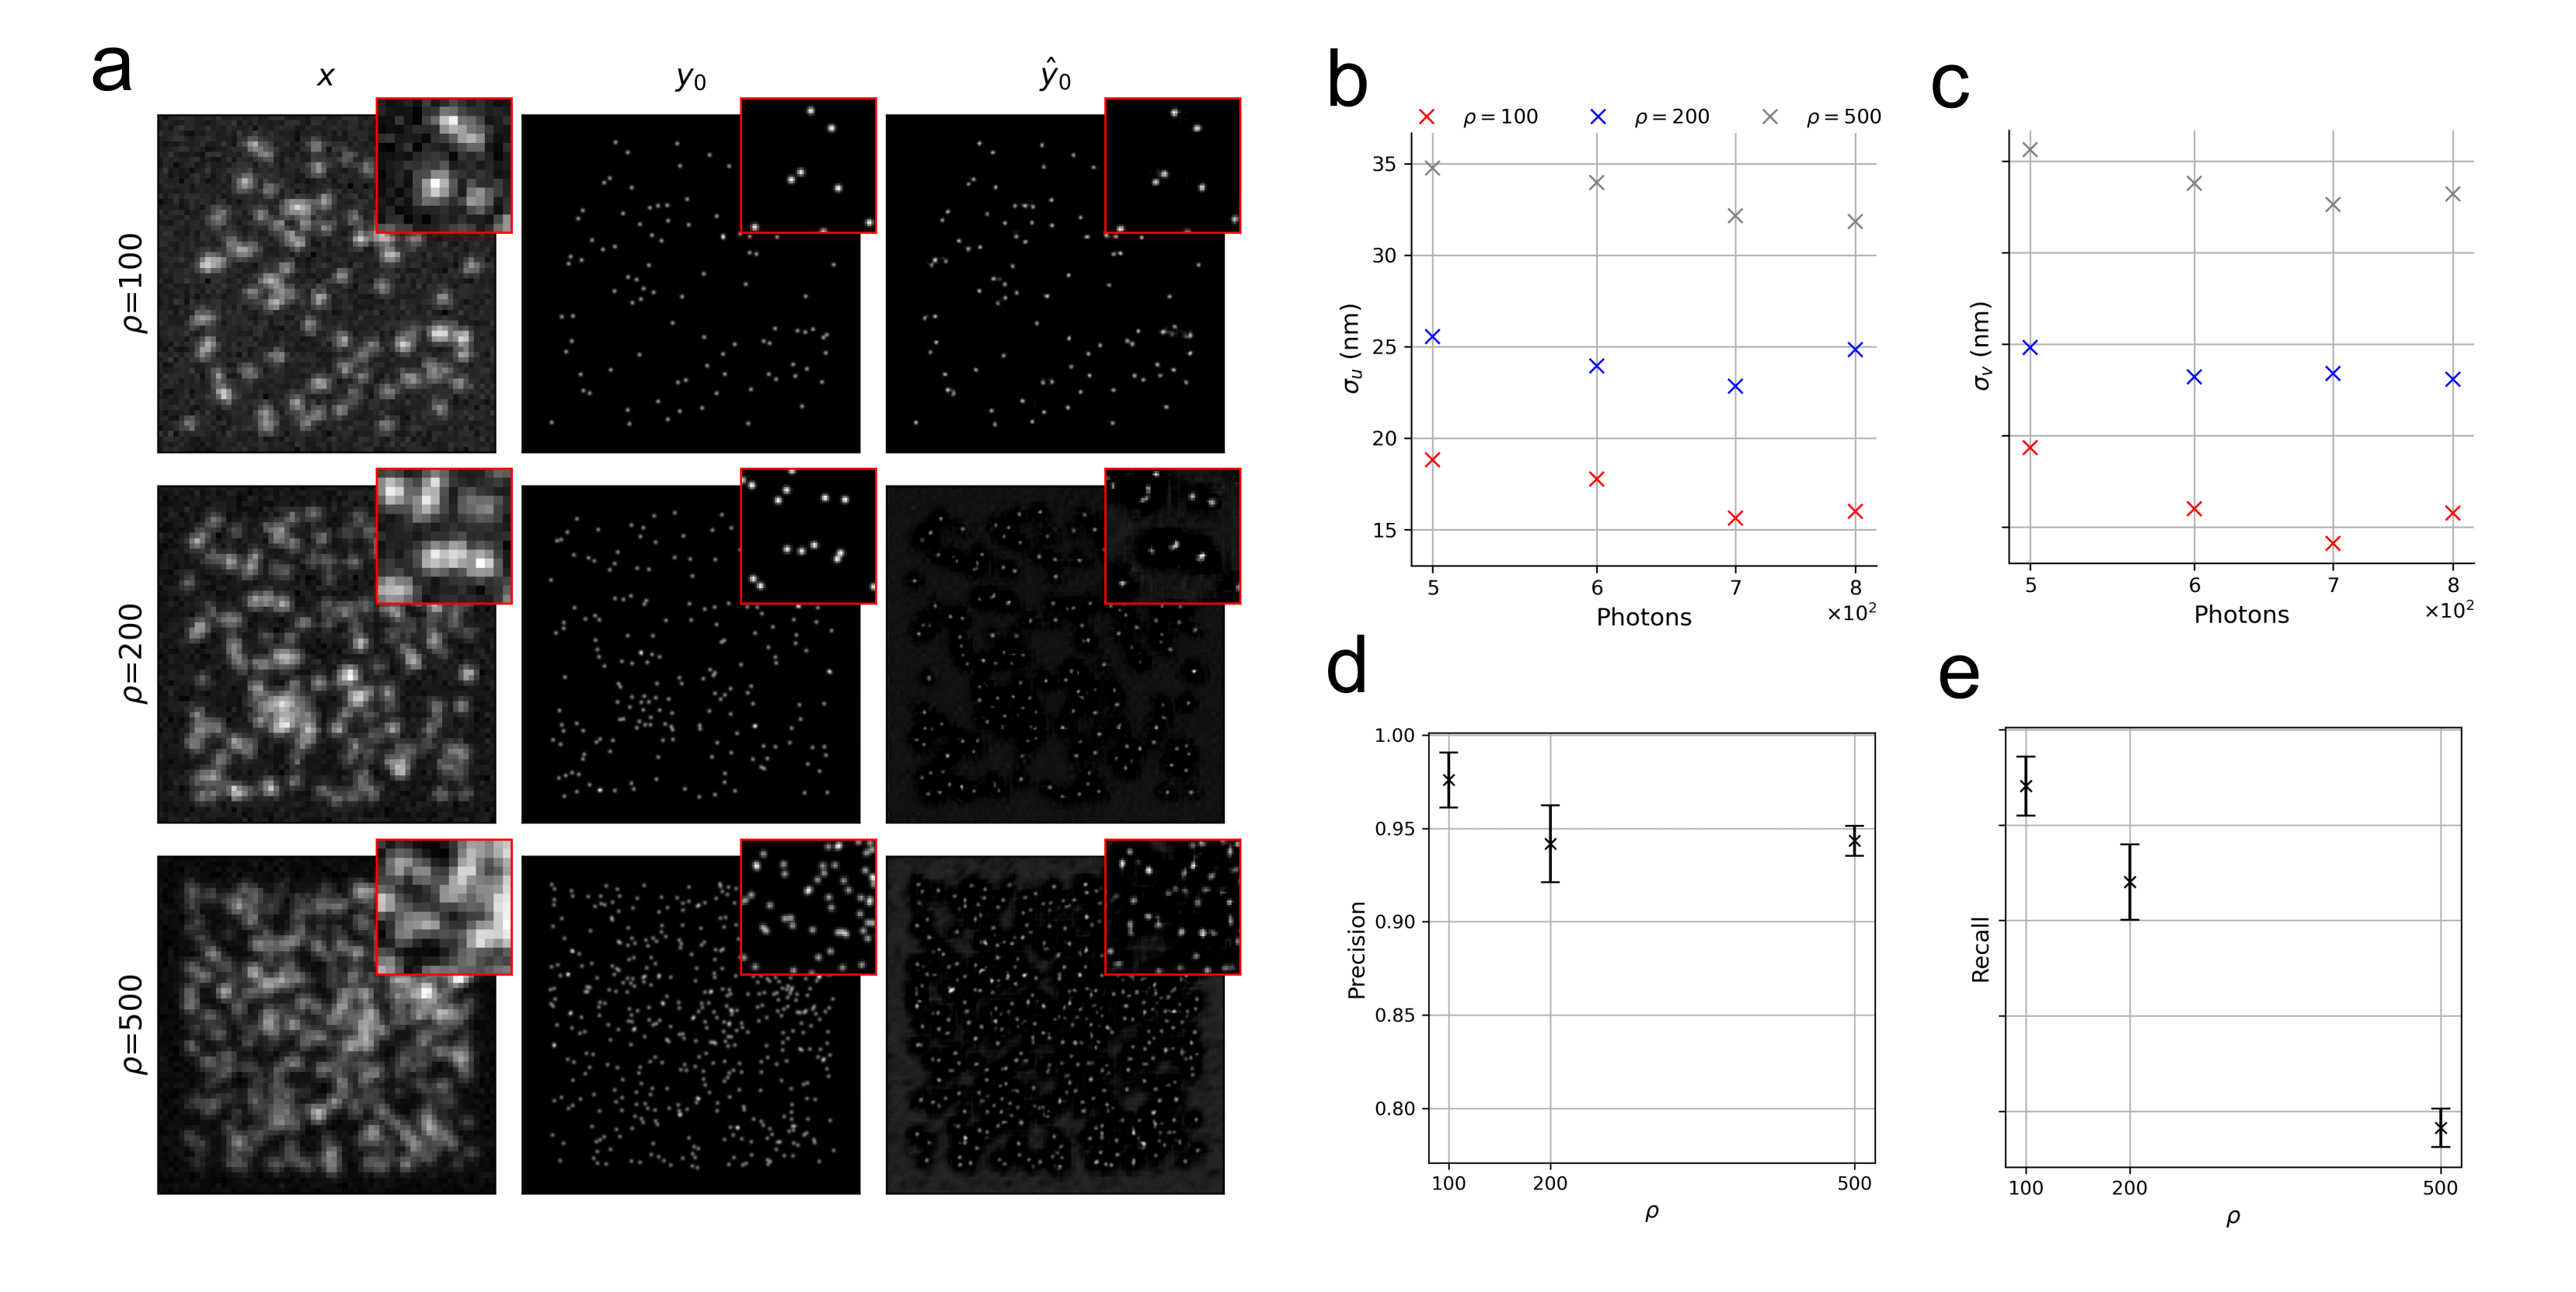
\includegraphics[scale=0.18]{/Users/cwseitz/git/cwseitz.github.io/docs/phd/ddpm/ddpm/media/Figure.png}
\caption{\textbf{Performance of conditional variational diffusion on simulated data}. (a) Example low resolution (left), high resolution (middle), and estimated high resolution (right) localization microscopy images at various densities (b,c) Localization uncertainty in the u and v directions as a function of incident photon count, for various densities. (d,c) Precision and recall of localized spots as a function of density.}
\label{fig:cvdmsim}
\end{figure}

%An important property of the forward process is that it admits sampling $\bold{y}_t$ at an arbitrary timestep $t$ in closed form \parencite{Ho2020}. Using the notation $\alpha_t := 1 - \beta_t$ and $\gamma_t := \prod_{s=1}^{t} \alpha_s$, we have $q(\bold{y}_t\lvert\bold{y}_0) = \mathcal{N} \left(\sqrt{\gamma_{t}} \bold{y}_{0}, (1 - \gamma_t)I \right)$ or $\bold{y}_{t} = \sqrt{\gamma_{t}}\bold{y}_{0} + \sqrt{1-\gamma_{t}}\bold{\epsilon}$ for $\epsilon \sim \mathcal{N}(0,I)$. The signal to noise ratio (SNR) as defined in \parencite{Kingma2023}, at a time step $t$ reads $\mathrm{SNR}_t = \gamma_{t}/(1-\gamma_{t})$.

%The usual procedure is then to learn a parametric representation of the \emph{reverse process}, and therefore generate samples of the latent $\bold{y}_{0}$ from  $p(\bold{y}_{0}\lvert\bold{x})$. Formally, $p_{\psi}(\bold{y}_{0}\lvert\bold{x}) = \int p_{\psi}(\bold{y}_{0:T}\lvert\bold{x})d\bold{y}_{1:T}$ where $\bold{y}_{t}$ is a latent representation with the same dimensionality of the data and $p_{\psi}(\bold{y}_{0:T}\lvert\bold{x})$ is a Markov process, starting from a noise sample $p_{\psi}(\bold{y}_{T}) = \mathcal{N}(0,I)$. Writing this Markov process gives

%\begin{equation}
%p_{\psi}(\bold{y}_{0:T}\lvert\bold{x}) = p_{\psi}(\bold{y}_{T})\prod_{t=1}^{T} p_{\psi}(\bold{y}_{t-1}\lvert\bold{y}_{t},\bold{x}) \;\;\; p_{\psi}(\bold{y}_{t-1}\lvert\bold{y}_{t},\bold{x}) = \mathcal{N}\left(\mu_{\psi}(\bold{y}_{t},\gamma_{t}),\beta_{t}I\right)
%\end{equation}

%where we reuse the variance schedule of the forward process \parencite{Ho2020}. From (5) it can be seen that the learnable parameter in the reverse process is the expectation of the transition $\mu_{\psi}$ where $\psi$ is a neural network. 

%Learning the reverse process can be approached by either regressing noise $\bold{\epsilon}$ from the forward process, or the true latent $\bold{y}_{0}$, as there is a deterministic relationship between them. We adopt the former for consistency with other work, and define $\psi$ as a neural denoising function which regresses the noise $\bold{\epsilon}$ from a noisy $\bold{y}_{t}$. A relation between the noise estimate $\epsilon_{\psi}$ and $\mu_{\psi}$ is given in the Appendix, which gives an intuition for sampling. The proposed sampling scheme is depicted in (Figure \ref{fig:fig60}). 


%\textbf{Variational Objective}. Following \parencite{Kingma2021}, we interpret the reverse process as a hierarchical generative model that samples a sequence of latents $\bold{y}_{t}$, with time running backward. Training of the model is achieved through the variational bound

%\begin{align}
%-\log p(\bold{y}_{0}) &\leq -\mathbb{E}_{q(\bold{y}_{1:T}\lvert\bold{y}_{0})} \log \left(\frac{p_{\psi}(\bold{y}_{1:T},\bold{y}_{0})}{q(\bold{y}_{1:T}\lvert\bold{y}_{0})}\right) \\
%&=  D_{KL}(q(\bold{y}_{T}\lvert\bold{y}_{0}) \lvert\lvert p(\bold{y}_{T})) + \mathbb{E}_{q(\bold{y}_{1}\lvert\bold{y}_{0})} \log p(\bold{y}_{0}\lvert\bold{y}_{1}) + \mathcal{L}_{T}
%\end{align}

%where we have omitted conditioning on the low-resolution $\bold{x}$ to simplify the notation. Note that, this is similar to a hierarchical VAE, but in a diffusion model $q(\bold{y}_{1:T}\lvert\bold{y}_{0})$ is fixed by the forward process rather than learned. The so-called diffusion loss $\mathcal{L}_{T}$ is shown in the Appendix, and is the term of interest as the first two terms do not contribute meaningfully to the loss \parencite{Ho2020}. Furthermore, it has become standard to use simplified forms of $\mathcal{L}_{T}$, such as a noise estimation loss, as this has shown superior performance. Importantly, $\mathcal{L}_{T}$ is simply a reweighted variant of a family of diffusion objectives \parencite{Kingma2021,Kingma2023}. We use the following Monte Carlo estimate of $\mathcal{L}_{T}$, which demonstrates that the variational bound can be written in terms of the common noise-estimation loss


%\begin{equation}
%\mathcal{L}_{T} = \mathbb{E}_{\epsilon\sim \mathcal{N}(0,I),t\sim U(1,T)}\left[\left(\frac{\mathrm{SNR}_{t-1}}{{\mathrm{SNR}_{t}}}-1\right)\lvert\lvert \bold{\epsilon}-\bold{\epsilon}_{\psi}\lvert\lvert_{2}^{2}\right]
%\end{equation}

%A full derivation of this objective is outlined in the Appendix. Note that $\mathrm{SNR}_{t}$ is monotonically decreasing with $t$, and thus $\frac{\mathrm{SNR}_{t-1}}{{\mathrm{SNR}_{t}}} = \frac{\gamma_{t-1}}{\gamma_{t}}\frac{1-\gamma_{t}}{1-\gamma_{t-1}} \geq 1$, ensuring $\mathcal{L}_{T}\geq 0$. In this paper, we choose to use a uniformly weighted loss and leave the exploration of the weighted loss to future work.

\subsection{Results}

\subsubsection{Localization error}

\begin{figure}[t]
\centering
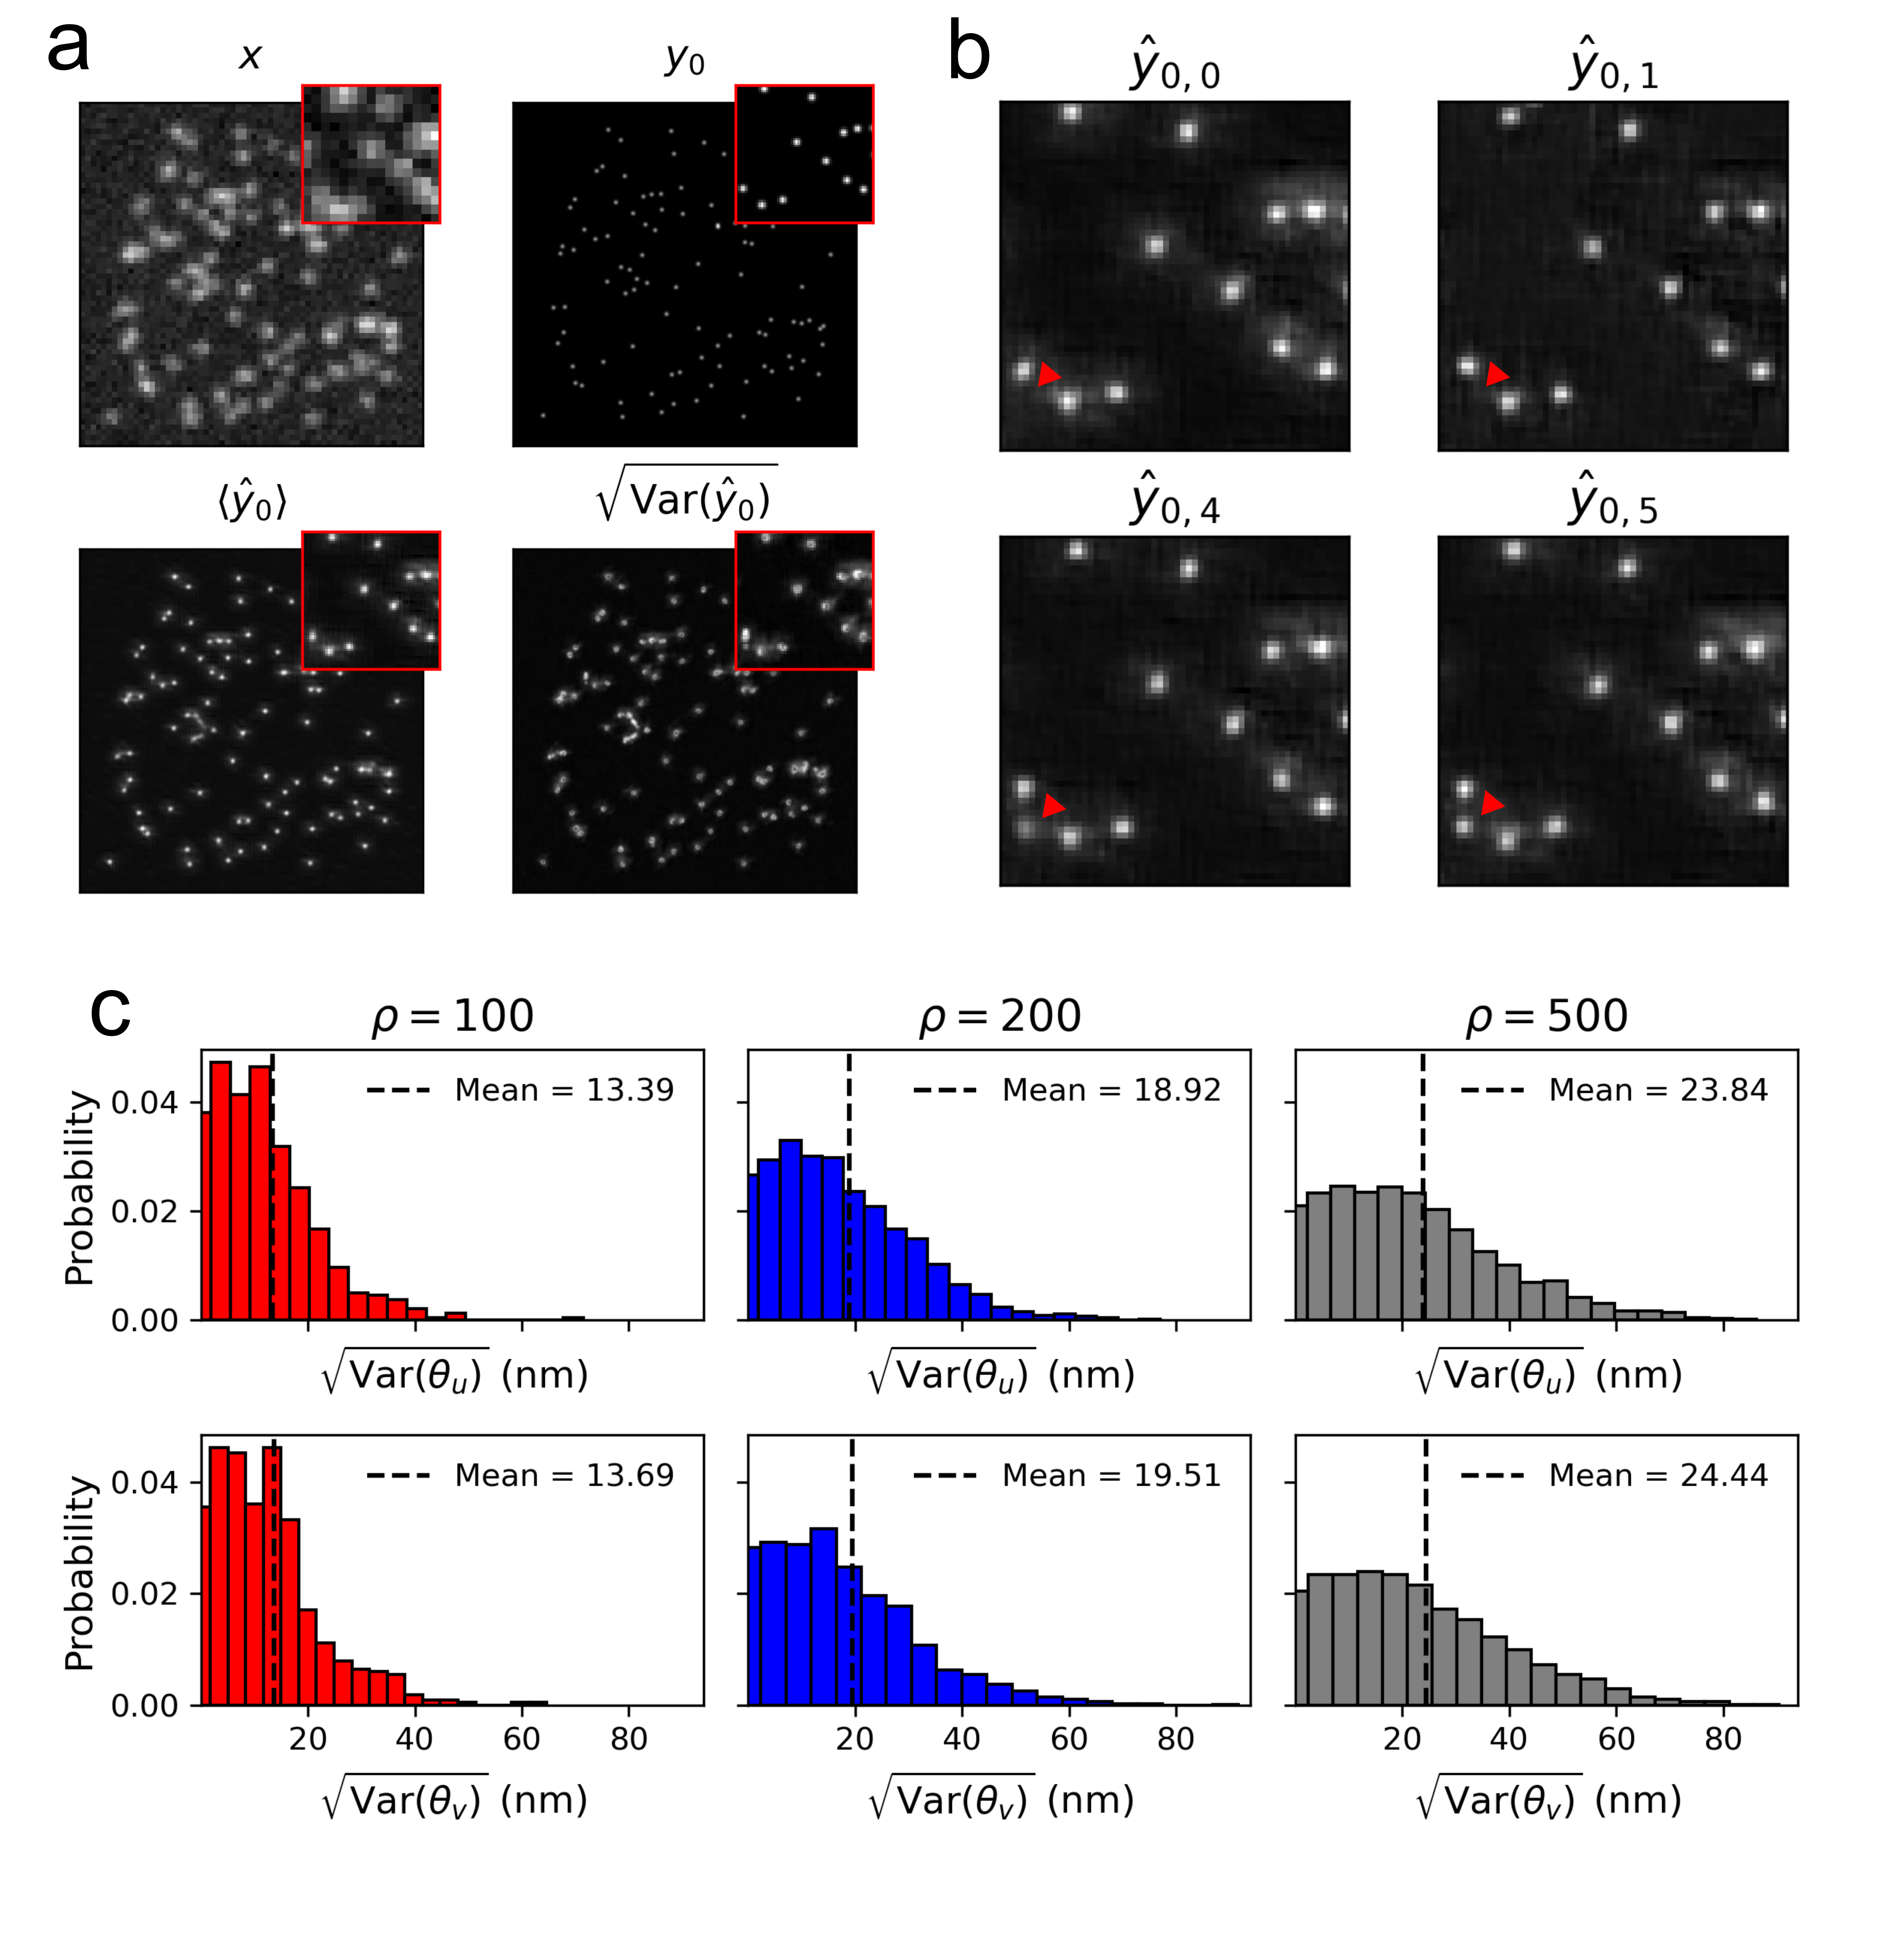
\includegraphics[scale=0.2]{/Users/cwseitz/git/cwseitz.github.io/docs/phd/ddpm/ddpm/media/Figure-2-1.png}
\caption{\textbf{Sample variation for simulated localization microscopy data} (a) Low-resolution, high resolution target, pixel-wise averaged prediction, and pixel-wise standard deviation (b) Samples from the diffusion model on high resolution images (c) Distribution of the standard deviation in emitter locations for various densities}
\label{fig:locobayes}
\end{figure}

\begin{figure}[t]
\centering
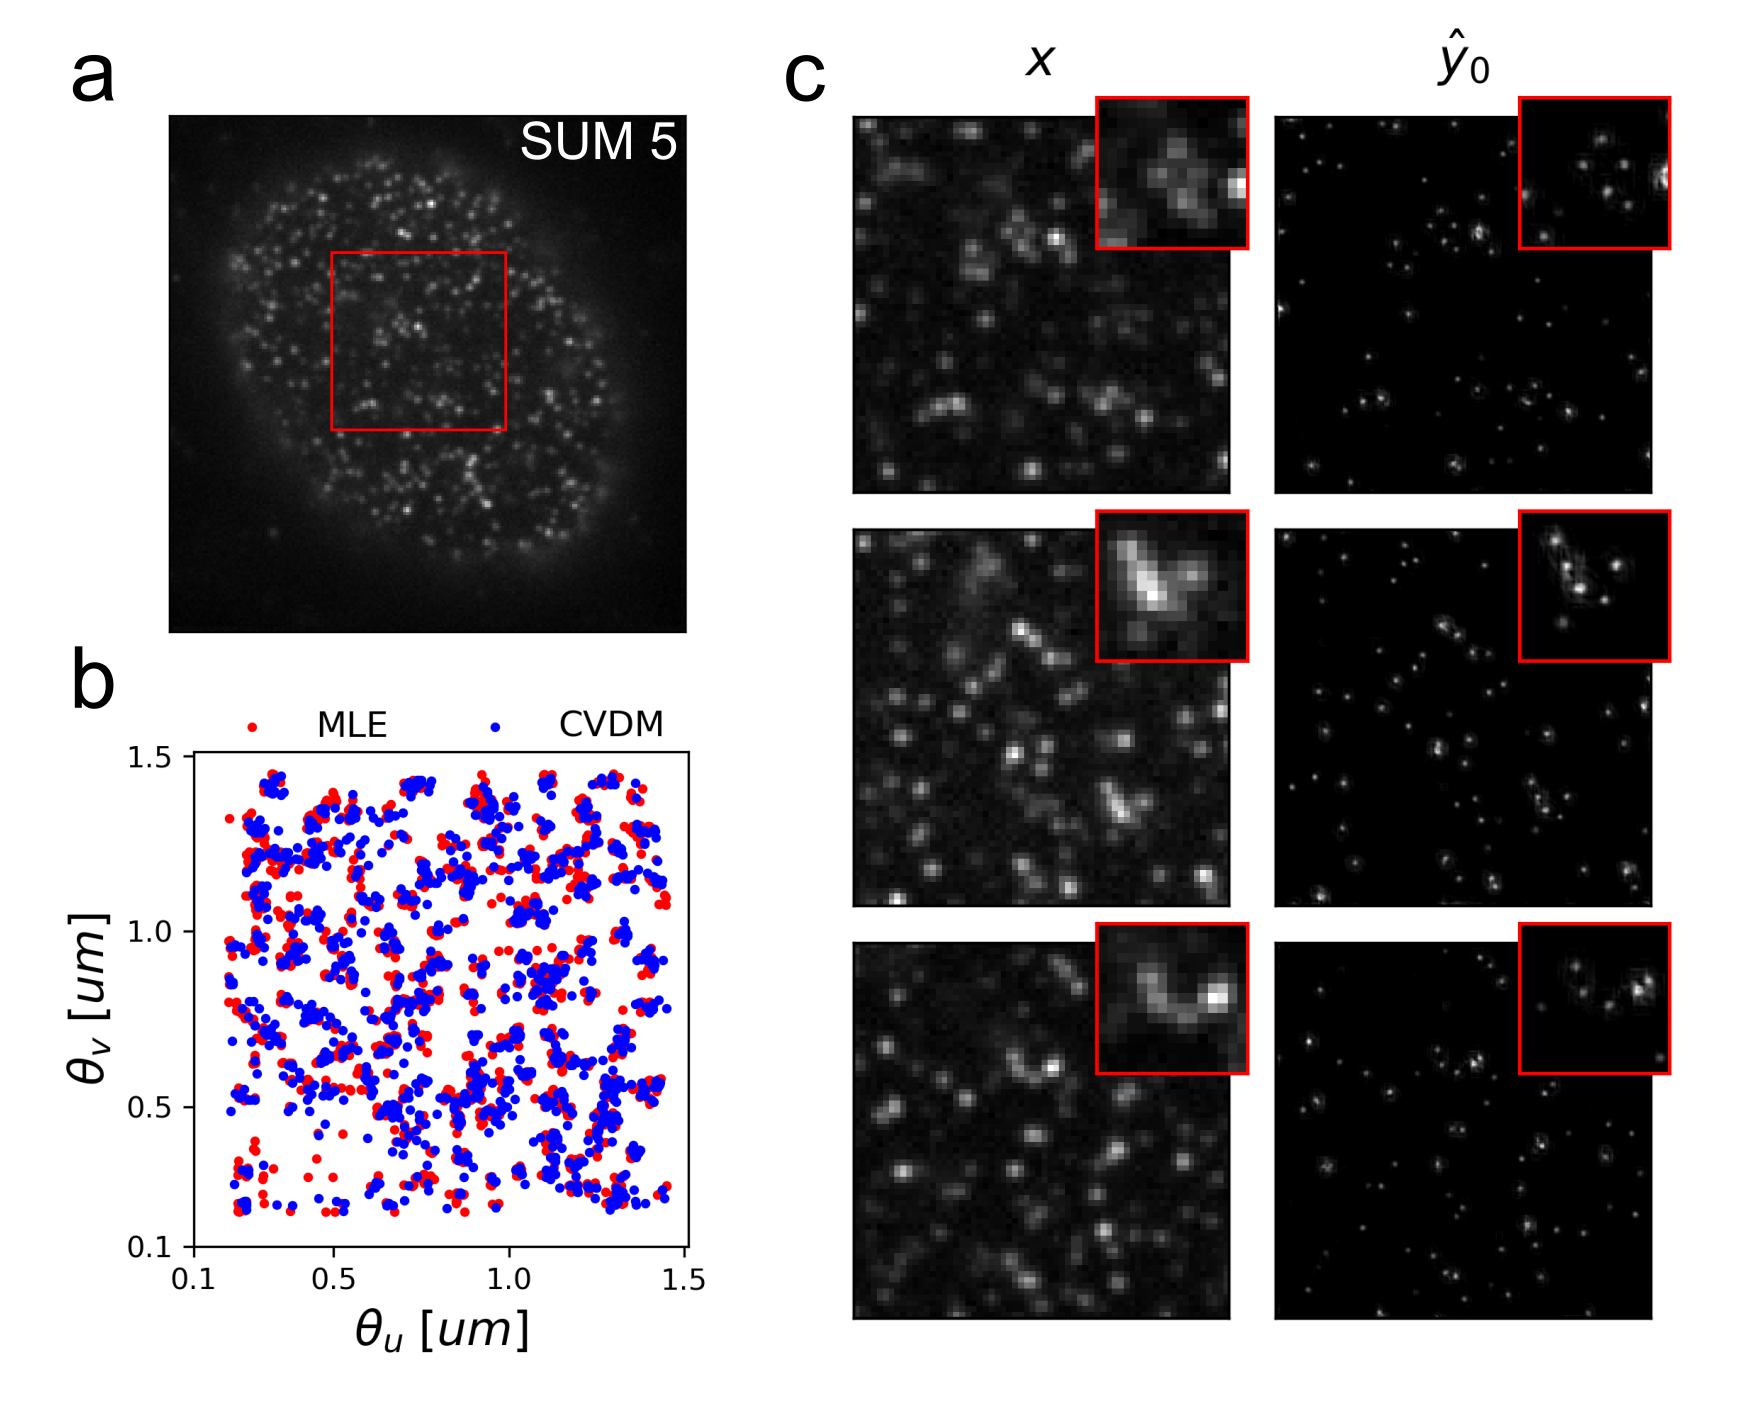
\includegraphics[scale=0.6]{/Users/cwseitz/git/cwseitz.github.io/docs/phd/ddpm/ddpm/media/Nup96.png}
\caption{\textbf{Super resolution of Nup96-mMaple} (a) Low-resolution frame of Nup96-mMaple obtained by summing five consecutive images (SUM 5) (b) Scattered coordinates found by maximum likelihood estimation on individual frames and the CVDM model on SUM 5 data. (c) Zoomed in regions from the data shown in (a) and corresponding samples from the model on high-resolution images}
\label{fig:nup96}
\end{figure}


To verify the localizations made by the diffusion model, we simulated localization microscopy datasets with various densities (Figure \ref{fig:cvdmsim}a). For a KDE predicted by the diffusion model, objects are detected using the Laplacian of Gaussian (LoG) detection algorithm, which permits more direct computation of localization error, compared to image similarity measures. Moreover, localization with sub-pixel precision can be easily implemented by identification of local maxima in the predicted KDE \parencite{Nehme2020}. A particular LoG localization in the KDE is paired to the nearest ground truth localization and is unpaired if a localization is not within 5 KDE pixels (125nm) of any ground truth localization. As expected, we find a density dependence to localization error in the $u$ and $v$ directions, and a weak relationship to signal to noise ratio, over the tested signal range (Figure \ref{fig:cvdmsim}b,c). In addition to localization error, we measure a density-dependent precision P = TP/(TP+FP) and precision P= TP/(TP+FN) where TP denotes true positive localizations, FP denotes false positive localizations, and FN denotes false negative localizations (Figure \ref{fig:cvdmsim}d,e). 

\subsubsection{Sample variation for simulated localization microscopy data}

Leveraging the ability of a diffusion process to model a distribution on high-resolution KDEs $p\left(\bold{y}_0\lvert \bold{x}\right)$ as opposed to a deterministic point estimate of $\bold{y}_0$, we assess the sample variation on simulated localization microscopy data. Upon inspection of samples from the diffusion model, we find that computing a pixel-wise average and standard deviation can summarize model predictions (Figure \ref{fig:locobayes}a). However, careful inspection of the individual samples can reveal the appearance/disappearance of predicted spots in the KDE across samples, expressing uncertainty in the number of spots in the KDE due to the many to one nature of image restoration tasks (Figure \ref{fig:locobayes}b). Furthermore, variation in the predicted locations of spots in the KDE is apparent, with more variation in higher density samples (Figure \ref{fig:locobayes}c). 

\subsubsection{Application to Nup96 localization microscopy data}

To validate the model on experimental localization microscopy data, we create dense images by summing five consecutive frames of sparsely labeled nuclear pore complex protein 96 (Nup96) tagged with mMaple \parencite{Speiser2021} (Figure \ref{fig:nup96}a). Scattered localizations predicted by the CVDM model showed strong agreement with standard maximum likelihood estimation (MLE) based fitting of single low-resolution frames (Figure \ref{fig:nup96}b). An obvious resolution enhancement was observed in CVDM predictions compared to low-resolution inputs (Figure \ref{fig:nup96}c). By matching CVDM predicted coordinates to MLE localizations using a search radius of 50nm, we find that over 99 percent of CVDM localizations match to a MLE coordinate. Moreover, ~60 percent of MLE coordinates were recovered, which is an acceptable result since MLE often detects the same fluorescent emitter multiple times with localization differences far below the minimum resolvable distance of CVDM. 


%All training data consits of low-resolution $20\times 20$ images, setting $\sigma_{\bold{x}}=0.92$ in units of low-resolution pixels, for consistency with common experimental conditions with a 60x magnification objective lens and numerical aperture (NA) of 1.4. We multiply $\omega_{k}$ by a constant $i_{0}=200$ for experiments for consistency with typical fluorophore emission rates. All KDEs have dimension $80\times 80$, are scaled between $[0,1]$, and are generated using $\sigma_{\bold{y}}=3.0$ pixels in the upsampled image (Figure \ref{fig:fig12}). For a typical CMOS camera, this results in KDE pixels with lateral dimension of $\approx 27\mathrm{nm}$. Initial coordinates $\theta$ were drawn uniformly over a two-dimensional disc with a radius of 7 low-resolution pixels.


%\begin{figure}
%\centering
%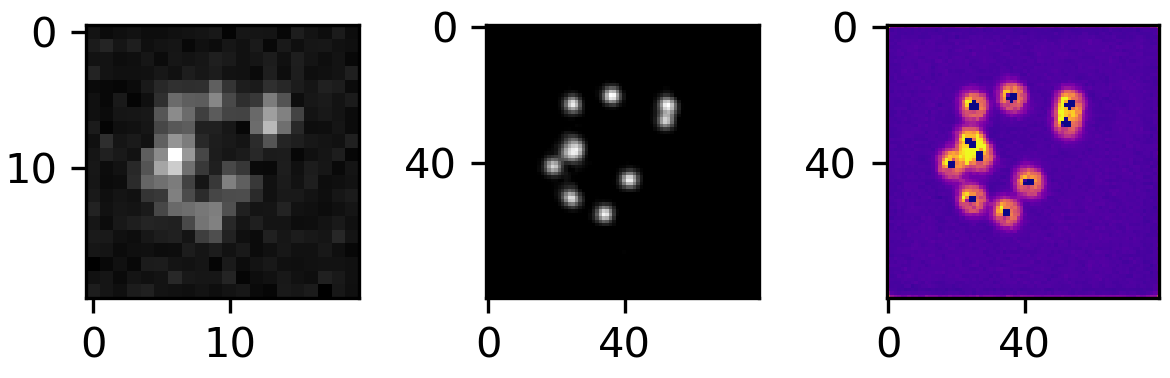
\includegraphics[scale=1.1]{/Users/cwseitz/git/cwseitz.github.io/docs/phd/ddpm/ddpm/media/Bayes.png}
%\caption{\textbf{Non cherry-picked estimation of marginal variances}. A low-resolution image $\bold{x}$ (left column) is transformed by $\phi$ to produce a KDE estimate $\hat{\bold{y}}$ (middle column) and a DDPM $\psi$ computes a map of marginal variances (right column)}
%\label{fig:fig12}
%\end{figure}


%\textbf{Localization RMSE}. In order to verify the initial predictions made by the augmentation model $\phi$, we simulated a dataset $(\bold{x}_i,\bold{y}_{0,i},\hat{\bold{y}}_{i})_{i=1}^{N}$ with $N=1000$. Objects in the KDE $\hat{\bold{y}}_{i}$  are detected using the Laplacian of Gaussian (LoG) detection algorithm \parencite{Kong2013}, which permits more direct comparison of model predictions to the Cramer-Rao lower bound on localization error, compared to other image similarity measures (Figure \ref{fig:fig15}). Localization is carried out from scale-space maxima directly in LoG, as opposed to fitting a model function to KDEs. A particular LoG localization in the KDE is paired to the nearest ground truth localization and is unpaired if a localization is not within 5 KDE pixels of any ground truth localization. In addition to localization error, we measure a precision $\mathrm{P = TP/(TP + FP)} = 1.0$ and recall $\mathrm{R = TP/(TP + FN)} = 0.85$, where $\mathrm{TP}$ denotes true positive localizations, $\mathrm{FP}$ denotes false positive localizations, and $\mathrm{FN}$ denotes false negative localizations.


%\textbf{Variational Diffusion}. We set $T = 100$ for all experiments and treat forward process variances $\beta_{t}$ as hyperparameters, with a linear schedule from $\beta_{0}=10^{-4}$ to $\beta_{T}=10^{-2}$.
%These constants were chosen to be small relative to ground truth KDEs, which are scaled to $[-1,1]$, ensuring that forward process distribution $\bold{y}_{T}\sim q(\bold{y}_{T}\lvert\bold{y}_{0})$ approximately matches the reverse process $\bold{y}_T\sim \mathcal{N}(0, I)$ at $t=T$. Example KD estimates from low-resolution images and the marginal variances obtained from sampling $N=100$ samples from $p_{\psi}(\bold{y}_{0}\lvert\bold{x})$ are shown in (Figure \ref{fig:fig12}). 


%\begin{figure}[t]
%\centering
%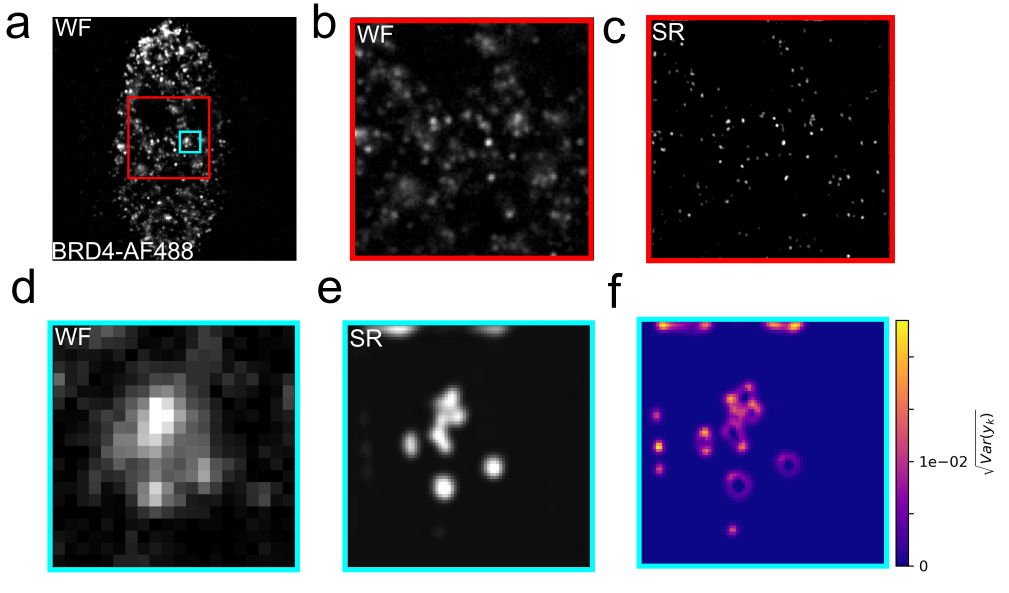
\includegraphics[scale=0.6]{/Users/cwseitz/git/cwseitz.github.io/docs/phd/ddpm/ddpm/media/BRD4/Deep2.png}
%\caption{\textbf{Super-resolution of BRD4 in a HeLa cell}. (a) Immunofluorescence image of BRD4 labeled with Alexa488 secondary antibody. (b) Zoomed widefield image of the inset highlighted in red and the super-resolved image (SR) after application of an encoder $\phi$. (c) Multi-step photobleaching profile of the inset highlighted in blue.}
%\label{fig:fig50}
%\end{figure}

%\textbf{Super Resolved Immunofluorescence}. To test our model in an experimental context, we performed immunofluorescence staining of endogeneous BRD4 protein in HeLa cells. Cells were grown in a 35mm dish and fixed with Formaldehyde in 1X PBS at room temperature incubator for 10 minutes, and then permeabilized in 70 percent ethanol. Cells were blocked for 1h with 0.3 percent (v/v) Triton-X100 (Sigma-Aldrich) and 5 percent (w/v) nonfat dry milk at 4C. Cells were incubated overnight at 4C using anti-BRD4 primary antibody (Cell Signaling, clone E2A7X; 1:1000) in blocker. Cells were then washed and stained with secondary antibodies for BRD4 (Cell Signaling Anti-Mouse IgG-Alexa488, 1:1000). For imaging, cells were imaged using a 60X 1.4NA oil immersion objective. Images were projected onto a CMOS Fusion camera (Hamamatsu) with a 40ms exposure time, using a 488nm continuous-wave laser aligned for oblique illumination. After background subtraction, the encoding network and diffusion model were used to estimate the super-resolved immunofluorescence image and its corresponding uncertainty (Figure \ref{fig:fig50}). 


\section{Discussion}

Application of the CVDM model to localization microscopy showed that the model is capable of not only enhancing the resolution of fluorescence images but also performing localization tasks. Indeed the model can maintain approximately 30nm localization error and high precision/recall on dense images. This result suggests that this model could be used to speed up localization microscopy acquisitions and enhance their resolution, while expressing uncertainty in the predicted outputs. 

Importantly, the principles underlying this method resonate across various fields, suggesting its potential applicability in domains beyond localization. For instance, the extension of similar techniques to general image processing tasks highlights the potential to address uncertainty in a wide range of applications in bioimaging or medical imaging. Moreover, the utilization of diffusion models for uncertainty estimation aligns with a broader trend in leveraging probabilistic frameworks for enhancing deep learning applications. By bridging these interdisciplinary boundaries, this method not only addresses a critical need in localization microscopy but also contributes to the advancement of uncertainty-aware deep learning methodologies.


\section{Appendix}

\subsection{Loss derivation in discrete-time}

The complete loss given in \parencite{Maggiora2023} reads

\begin{equation}
\mathcal{L} = \mathcal{L}_{\mathrm{prior}} + \mathcal{L}_{\infty} + \alpha\mathcal{L}_{\gamma} + \mathcal{L}_{\beta}
\end{equation}

where $\alpha$ is a constant controlling the contribution of $\mathcal{L}_{\gamma}$ to the total loss. We now derive the first two terms and discuss the latter two terms in the following section. Similar derivations can be found in \parencite{Maggiora2023,Kingma2021,Ribeiro2024}. The approach starts with writing the ELBO for a discrete-time diffusion model, and then taking the limit $T\rightarrow \infty$. In the discrete-time formalism time is indexed as $t\in \{1,2,...,T\}$. The ELBO reads

\begin{align*}
-\log p(\bold{y}_{0}) &\leq - \mathbb{E}_{q(\bold{y}_{1:T}\lvert\bold{y}_{0})} \log \frac{p(\bold{y}_{0:T})}{q(\bold{y}_{1:T}\lvert\bold{y}_{0})}\\
&= -\mathbb{E}_{q(\bold{y}_{1:T}\lvert\bold{y}_{0})} \log \frac{p(\bold{y}_{T})p(\bold{y}_0\lvert\bold{y}_1) \prod_{t=2}^{T}p(\bold{y}_{t-1}\lvert\bold{y}_t)}{q(\bold{y}_T\lvert\bold{y}_0)\prod_{t=2}^{T}q(\bold{y}_{t-1}\lvert\bold{y}_t,\bold{y}_0)}\\
&= -\mathbb{E}_{q(\bold{y}_{1:T}\lvert\bold{y}_{0})} \left[ p(\bold{y}_0\lvert\bold{y}_1) + \log \frac{p(\bold{y}_{T})}{q(\bold{y}_T\lvert\bold{y}_0)} + \sum_{t=2}^{T} \log \frac{p(\bold{y}_{t-1}\lvert\bold{y}_t)}{q(\bold{y}_{t-1}\lvert\bold{y}_t,\bold{y}_0)}\right]\\
&= -\mathbb{E}_{q(\bold{y}_{1:T}\lvert\bold{y}_{0})} \left[ p(\bold{y}_0\lvert\bold{y}_1)\right] + D_{KL}\left(q(\bold{y}_T\lvert\bold{y}_0) \lvert\lvert p(\bold{y}_{T})\right) \\
&+ \sum_{t=2}^{T} \mathbb{E}_{q(\bold{y}_{t}\lvert\bold{y}_{0})} D_{KL}\left(q(\bold{y}_{t-1}\lvert\bold{y}_t,\bold{y}_0)\lvert\lvert p(\bold{y}_{t-1}\lvert\bold{y}_t) \right)
\end{align*}

As before, we omit conditioning on $\bold{x}$ to simplify the notation. The first term is typically ignored, as it does not contribute meaningfully to the loss \parencite{Ribeiro2024}. Therefore we are last two terms, called the prior loss $\mathcal{L}_{\mathrm{prior}}$ and diffusion loss $\mathcal{L}_{T}$. The former is straightforward to optimize using analytical expressions \parencite{Maggiora2023}. Furthermore, define $\beta_{t}$ as the variance at time step $t$, $\alpha_{t}=1-\beta_{t}$ and $\gamma_{t}=\prod_{t}\alpha_{t}$. The latter KL-divergence of $q$ and $p$ is between two Gaussians with identical variances $\sigma^{2} = \frac{(1-\gamma_{t-1})(1-\alpha_{t})}{1-\gamma_{t}}$, and expectations

\begin{align*}
\mu = \frac{\sqrt{\gamma_{t-1}}(1-\alpha_{t})}{1-\gamma_{t}}\bold{y}_{0}+ \frac{\sqrt{\alpha_{t}}(1-\gamma_{t-1})}{{1-\gamma_{t}}}\bold{y}_{t} \quad \hat{\mu} = \frac{\sqrt{\gamma_{t-1}}(1-\alpha_{t})}{1-\gamma_{t}}\hat{\bold{y}}_{0}+ \frac{\sqrt{\alpha_{t}}(1-\gamma_{t-1})}{{1-\gamma_{t}}}\bold{y}_{t}
\end{align*}

for a fixed noise schedule \parencite{Saharia2021}. Therefore, we have

\begin{align*}
D_{KL}\left(q(\bold{y}_{t-1}\lvert\bold{y}_t,\bold{y}_0)\lvert\lvert p(\bold{y}_{t-1}\lvert\bold{y}_t) \right) &= \frac{1}{2\sigma^{2}} \lvert\lvert \mu - \hat{\mu} \lvert\lvert_{2}^{2} \\
&= \frac{1}{2}\frac{\gamma_{t-1}(1-\alpha_{t})}{(1-\gamma_{t-1})(1-\gamma_{t})}\lvert\lvert \bold{y}_{0} - \hat{\bold{y}}_{0} \lvert\lvert_{2}^{2}\\
&= \frac{1}{2}\frac{\gamma_{t-1}((1-\gamma_{t})-\alpha_{t}(1-\gamma_{t-1}))}{(1-\gamma_{t-1})(1-\gamma_{t})}\lvert\lvert \bold{y}_{0} - \hat{\bold{y}}_{0} \lvert\lvert_{2}^{2}\\
&= \frac{1}{2}\frac{\gamma_{t-1}((1-\gamma_{t})-\frac{\gamma_{t}}{\gamma_{t-1}}(1-\gamma_{t-1}))}{(1-\gamma_{t-1})(1-\gamma_{t})}\lvert\lvert \bold{y}_{0} - \hat{\bold{y}}_{0} \lvert\lvert_{2}^{2}\\
&= \frac{1}{2}\left(\frac{\gamma_{t-1}}{1-\gamma_{t-1}}-\frac{\gamma_{t}}{1-\gamma_{t}}\right)\lvert\lvert \bold{y}_{0} - \hat{\bold{y}}_{0} \lvert\lvert_{2}^{2}\\
&= \frac{1}{2}\left(\mathrm{SNR}_{t-1}-\mathrm{SNR}_{t}\right)\lvert\lvert \bold{y}_{0} - \hat{\bold{y}}_{0} \lvert\lvert_{2}^{2}
\end{align*}

%Reparameterizing the loss in terms of the noise, using $\lvert\lvert \bold{y}_{0} - \hat{\bold{y}}_{0} \lvert\lvert_{2}^{2} = \frac{1-\gamma_{t}}{\gamma_{t}}\lvert\lvert \bold{\epsilon}_{0} - \epsilon_{\psi} \lvert\lvert_{2}^{2}$ \parencite{Ribeiro2024}, we arrive at 

%\begin{equation}
%\mathcal{L}_{T} = \frac{1}{2}\sum_{t=2}^{T} \mathbb{E}_{q(\bold{y}_{t}\lvert\bold{y}_{0})}\left(\frac{\mathrm{SNR}_{t-1}}{{\mathrm{SNR}_{t}}}-1\right)\lvert\lvert \bold{\epsilon}-\bold{\epsilon}_{\psi}\lvert\lvert_{2}^{2}
%\end{equation}

where we have defined $\mathrm{SNR}_{t} = \frac{\gamma_{t}}{1-\gamma_{t}}$. Putting it all together gives that 

\begin{equation}
\mathcal{L}_{T} = \frac{1}{2}\sum_{t=2}^{T} \mathbb{E}_{q(\bold{y}_{t}\lvert\bold{y}_{0})}\left(\mathrm{SNR}_{t-1}-\mathrm{SNR}_{t}\right)\lvert\lvert \bold{y}_{0} - \hat{\bold{y}}_{0} \lvert\lvert_{2}^{2}
\end{equation}

Using a Monte Carlo estimate of $\mathcal{L}_{T}$ \parencite{Kingma2023} which optimizes random terms of the summation to avoid calculating all terms simultaneously, we arrive at the objective written in the main text (8)

%\begin{equation}
%\mathcal{L}_{T} = \mathbb{E}_{\epsilon\sim \mathcal{N}(0,I),t\sim U(1,T)}\left[\left(\frac{\mathrm{SNR}_{t-1}}{{\mathrm{SNR}_{t}}}-1\right)\lvert\lvert \bold{\epsilon}-\bold{\epsilon}_{\psi}\lvert\lvert_{2}^{2}\right]
%\end{equation}

\begin{equation}
\mathcal{L}_{T} = \frac{T-1}{2} \mathbb{E}_{\boldsymbol{\epsilon}\sim \mathcal{N}(0,I),t\sim U(1,T)}\left(\mathrm{SNR}_{t-1}-\mathrm{SNR}_{t}\right)\lvert\lvert \bold{y}_{0} - \hat{\bold{y}}_{0} \lvert\lvert_{2}^{2}
\end{equation}

Taking the limit $T\rightarrow\infty$, this becomes:

\begin{align*}
\mathcal{L}_\infty &= -\frac{1}{2} \mathbb{E}_{\boldsymbol{\epsilon} \sim \mathcal{N}(0,I)} \int_{0}^{1} \mathrm{SNR}'(t) \lvert\lvert \bold{y}_{0} - \hat{\bold{y}}_{0} \lvert\lvert_{2}^{2} dt \\
&= -\frac{1}{2} \mathbb{E}_{\boldsymbol{\epsilon} \sim \mathcal{N}(0,I),t \sim U([0,1])} \left[\mathrm{SNR}'(t) \lvert\lvert \bold{y}_{0} - \hat{\bold{y}}_{0} \lvert\lvert_{2}^{2}\right]
\end{align*}

Moving to continuous time is a critical step, as it has been shown that increasing the number of time steps $T$ should reduce to diffusion loss \parencite{Kingma2023}. This diffusion loss is often recast as a noise estimation loss by making use of the relationship given in (3.9). Indeed, after some algebra we find that

\begin{equation*}
\mathcal{L}_\infty = \frac{1}{2} \mathbb{E}_{\boldsymbol{\epsilon} \sim \mathcal{N}(0,I),t \sim U([0,1])} \lvert\lvert \boldsymbol{\epsilon} - \hat{\boldsymbol{\epsilon}} \lvert\lvert_{2}^{2}
\end{equation*}

which gives us the continuous-time diffusion loss used in the complete objective $\mathcal{L}$. Note that in the continuous-time framework, time is instead uniformly sampled over an interval $[0,1]$. 

\subsection{Regularization of the noise schedule}

The second two terms of $\mathcal{L}$, namely $\mathcal{L}_{\gamma}$ and $\mathcal{L}_{\beta}$, act to constrain the learned noise schedule. Their full mathematical justification is out of the scope of this thesis and the following is a brief introduction to the full argument given in \parencite{Maggiora2023}. In the continuous-time framework the noise schedule is given now by a continuous function $\gamma(t,\bold{x})$. A first constraint is placed on $\gamma(t,\bold{x})$ in order to preserve the similarity between discrete and continuous time implementations 

\begin{equation*}
\mathcal{L}_{\gamma} = \lvert\lvert \gamma''(t,\bold{x}) \lvert\lvert_{2}^{2}
\end{equation*}

Furthermore, in their generalization to continuous time, \parencite{Maggiora2023} introduced the continuous function $\beta(t,\bold{x})$ such that

\begin{equation*}
\frac{\partial \gamma(t,\bold{x})}{\partial t} = -\beta(t,\bold{x})\gamma(t,\bold{x})
\end{equation*}

where $\beta(t,\bold{x})$ is a separable function of time and space: $\beta(t,\bold{x}) = \tau_{\Theta}(t)\lambda_{\Phi}(\bold{x})$, which are computed by neural networks $\Theta$ and $\Phi$, respectively. The equation above acts as a constraint on the noise schedule,    ensuring the diffusion process is smooth and free of sudden jumps

\begin{equation*}
\mathcal{L}_\beta = \mathbb{E}_{t \sim U([0,1])} \left[
\lVert \frac{\partial \gamma(t,\bold{x})}{\partial t} + \beta(t,\bold{x})\gamma(t,\bold{x}) \rVert_2^2
+ \lVert \gamma(0,\bold{x}) - 1 \rVert_2^2 
+ \lVert \gamma(1,\bold{x}) - 0 \rVert_2^2
\right]
\end{equation*}

The last two terms codify the soft constraints $\gamma(0,\bold{x})= 1$ and $\gamma(1,\bold{x}) = 0$, which help to ensure that the forward process starts at $\bold{y}_{0}$ and ends in a standard Gaussian variable \parencite{Maggiora2023}. 

\subsection{Sampling}

Sampling from the reverse process $p(\bold{y}(t)\lvert\bold{y}(t+\Delta t)$ is achieved by estimation of the noise $\hat{\boldsymbol{\epsilon}}$ from $\bold{y}_{t}$ by the denoising model, and therefore estimation of $\bold{y}_{0}$

\begin{equation}
\hat{\mathbf{y}}_{0} = \frac{1}{\sqrt{\gamma(t, \mathbf{x})}} \left( \mathbf{y}(t) - \sqrt{1-\gamma(t, \mathbf{x})} \, \hat{\boldsymbol{\epsilon}} \right)
\end{equation}

followed by sampling from the forward process $\bold{y}(t) \sim q(\bold{y}(t)\lvert\hat{\bold{y}}_{0}) = \mathcal{N}(\sqrt{\gamma(t,\bold{x})},(1-\gamma(t,\bold{x}))I)$. 

%Sampling from the reverse process $p_{\psi}(\bold{y}_{t-1}\lvert\bold{y}_{t},\bold{x})$ is achieved by estimation of the noise $\hat{\epsilon}$ from $\bold{y}_{t}$ by the denoising model $\psi$, and therefore estimation of $\bold{y}_{0}$

%\begin{equation}
%\hat{\bold{y}}_{0} = \frac{1}{\sqrt{\gamma_{t}}}(\bold{y}_{t} - \sqrt{1-\gamma_{t}}\hat{\epsilon})
%\end{equation}

%followed by sampling from the forward process $\bold{y}_{t-1} \sim q(\bold{y}_{t-1}\lvert\hat{\bold{y}}_{0}) = \mathcal{N}(\sqrt{\gamma_{t-1}},(1-\gamma_{t-1})I)$. 



%\begin{figure}[t]
%\centering
%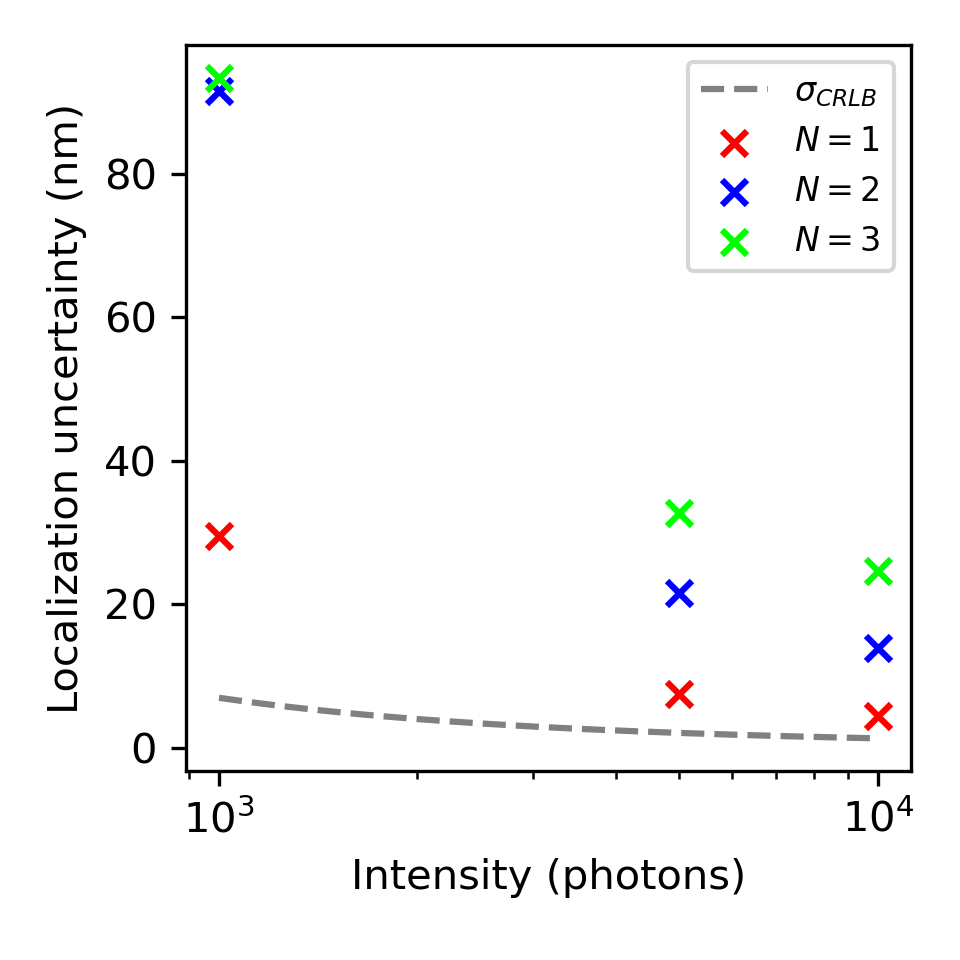
\includegraphics[scale=0.7]{/Users/cwseitz/git/cwseitz.github.io/docs/phd/ddpm/ddpm/media/Errors.png}
%\caption{\textbf{Localization errors of the trained model $\phi$}. The Cramer-Rao lower bound is shown in red, computing by taking the diagonal elements of $I^{-1}(\theta)$.}
%\label{fig:fig15}
%\end{figure}


%\subsection{Neural network architectures}

%\begin{figure}[t]
%\centering
%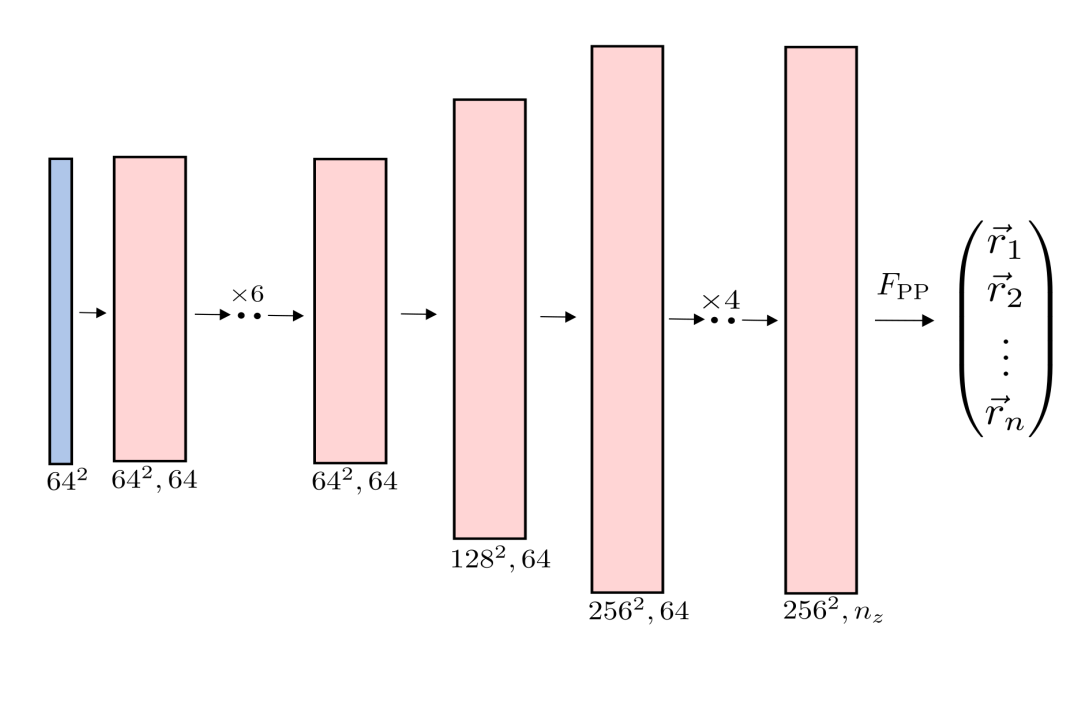
\includegraphics[scale=0.4]{/Users/cwseitz/git/cwseitz.github.io/docs/phd/ddpm/ddpm/media/DeepSTORM.png}
%\caption{\textbf{Architecture of the augmenation model $\phi$}. A $20\times 20$ single-channel image is processed by eight convolutional blocks followed by a 4x upsampling module utilizing linear interpolation and a refinement module with six convolutional blocks. The number of output channels $n$ is set to one, but can be set to values greater than one to obtain axial resolution in three-dimensional localization microscopy}
%\label{fig:fig13}
%\end{figure}


%\begin{figure}[t]
%\centering
%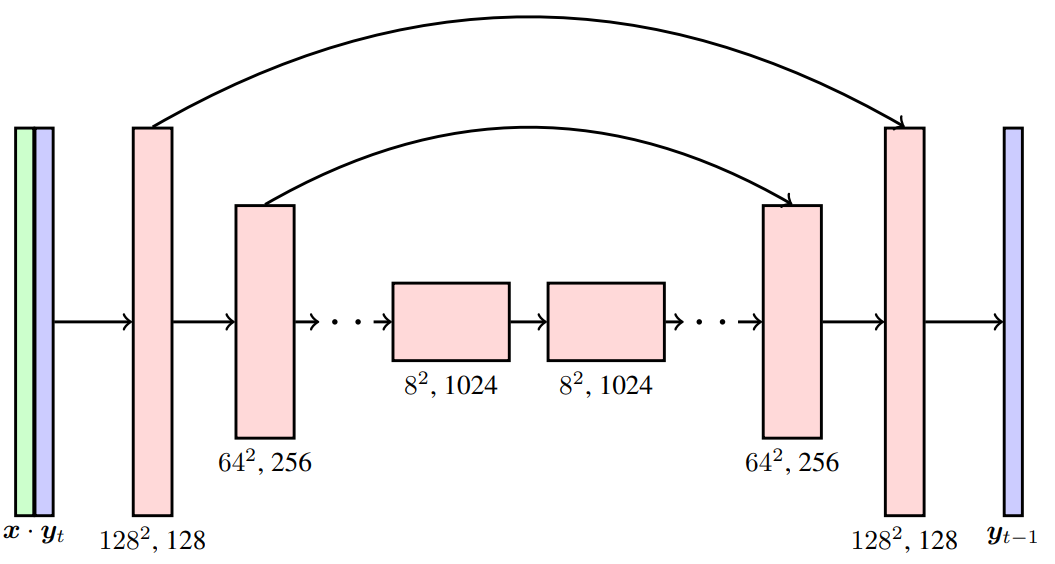
\includegraphics[scale=1.5]{/Users/cwseitz/git/cwseitz.github.io/docs/phd/ddpm/ddpm/media/DiffusionArch.png}
%\caption{\textbf{Architecture of the denoising diffusion model}. A U-Net style architecture with channel multipliers of [1,2,4,8,16] downsamples and then upsamples the input image $\bold{y}_{t}$ to estimate $\bold{y}_{t-1}$}
%\label{fig:fig14}
%\end{figure}

%\textbf{DeepSTORM CNN $\phi$}. The DeepSTORM CNN (Figure \ref{fig:fig13}), for 3D localization, can be viewed as a deep kernel density estimator, reconstructing kernel density estimates $\bold{y}$ from low-resolution inputs $\bold{x}$. We utilize a simplified form of the original architecture \parencite{Nehme2020} for 2D localization, which we denote $\phi$ in this paper, which consists of three main modules: a multi-scale context aggregation module, an upsampling module, and a prediction module. For context aggregation, the architecture utilizes dilated convolutions to increase the receptive field of each layer. The upsampling module is then composed of two consecutive 2x resize-convolutions, computed by nearest-neighbor interpolation, to increase the lateral resolution by a factor of 4. Additional details regarding this architecture can be found in the original paper \cite{Nehme2020}. The terminal prediction module contains three additional convolutional blocks for refinement of the upsampled image, followed by an element-wise HardTanh. The architecture is trained using the objective $\mathcal{L}_{\phi} = \frac{1}{N}\sum_{n=1}^{N} (\bold{y}_{0,n}-\bold{\hat{y}}_{n})^{2}$. 

%\textbf{DDPM $\psi$}. To represent the reverse process, we used a DDPM architecture (Figure \ref{fig:fig14}) originally proposed in \parencite{Saharia2021}. We chose the U-Net backbone to have channel multipliers $[1,2,4,8,8]$ in the downsampling and upsampling paths of the architecture. In this architecture, parameters are shared across time, which is specified to the network using the Transformer sinusoidal position embedding, and uses self-attention at the $16 \times 16$ feature map resolution. To condition the model on the input $\bold{\hat{y}}$, we concatenate the $\bold{\hat{y}}$ estimated by DeepSTORM along the channel dimension, which are scaled to $[0,1]$, with $\bold{y}_T\sim \mathcal{N}(0, I)$. Others have experimented with more sophisticated methods of conditioning, but found that the simple concatenation yielded similar generation quality \parencite{Saharia2021}. 

\ProvidesFile{ch4.tex}[Chapter4]

\chapter{FLUORESCENCE NANOSCOPY IN THE STUDY OF CHROMATIN ORGANIZATION}
\ix{physics//Physics appendix}

\section{Background}

Chromatin is a complex and dynamic structure that packages eukaryotic DNA with histones. The higher-order structure of chromatin is highly non-random and plays an important role in regulation of genomic functions such as gene expression, DNA synthesis, and DNA repair. Chromatin structure is strictly controlled and constantly remodeled as cells differentiate, divide, and respond to genomic insults \parencite{Auerbach2009,Chien2009,Clapier2009,Misteli2007,Vidi2014}.

\begin{figure}[t]
\centering
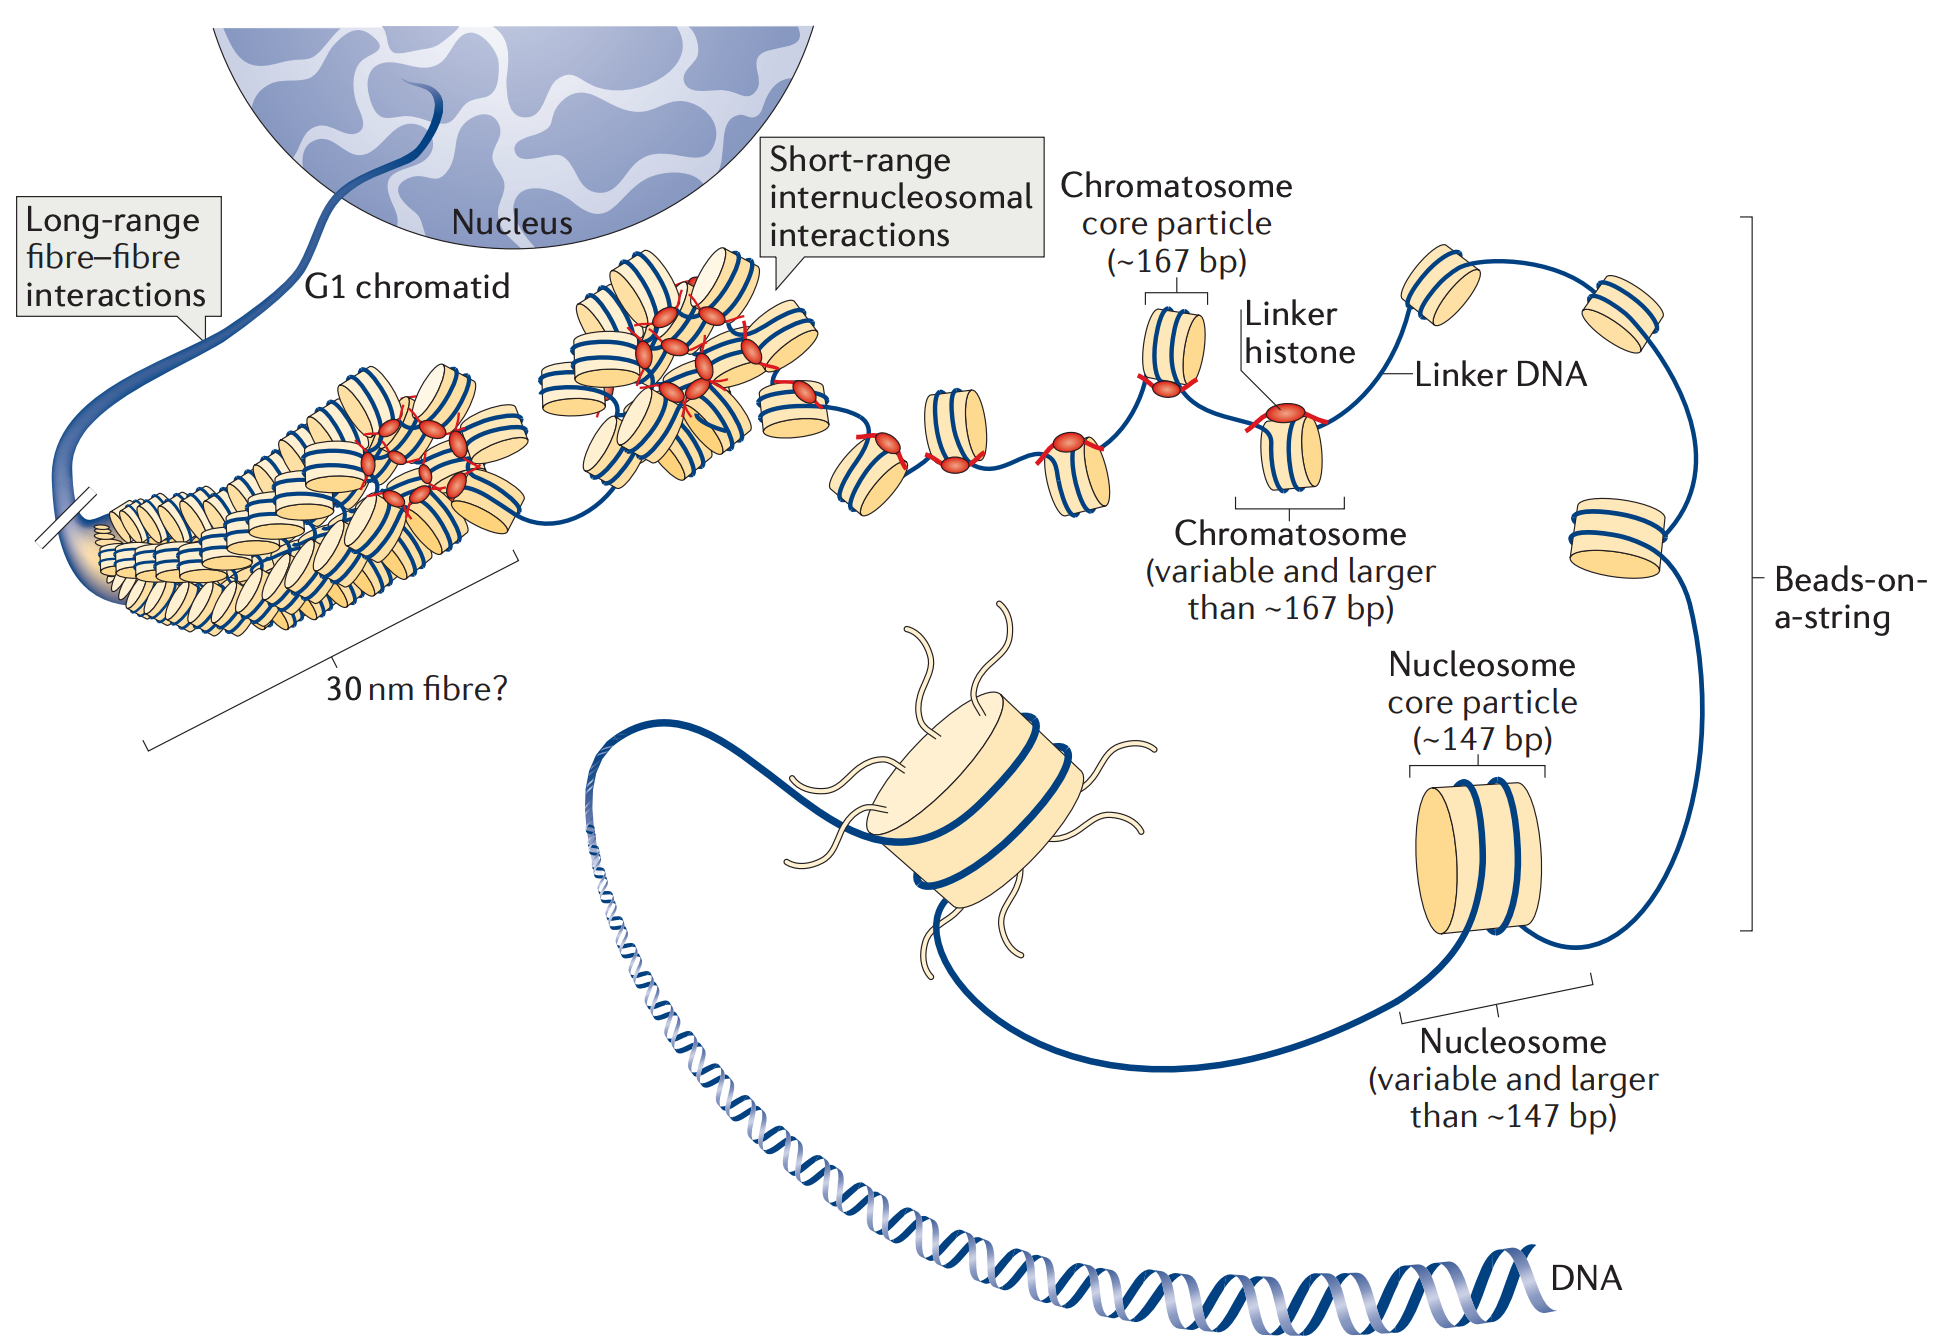
\includegraphics[width=13cm]{media/Chromatin.png}
\caption{\textbf{The hierarchical structure of chromatin} DNA compaction within the interphase nucleus occurs through multiple levels of histone-dependent interactions. This includes the formation of the nucleosome core particle, strings of nucleosomes, the chromatosome core particle, the debated 30nm fibers, and the association of individual fibers, which eventually produces tertiary structures. Retrieved from \parencite{Fyodorov2018}.}
\label{fig:fig16}
\end{figure}

While DNA linearly encodes genetic information, serving as a template for RNA and protein production, the spatial and temporal organization of chromatin plays a fundamental role in determining intranuclear activities and gene stability \parencite{Cuvier2017,Dion2013}. For example, local structural fluctuations in nucleosomes on microsecond to second timescales transiently expose buried DNA sites, thus providing temporary access to interaction sites \parencite{Choy2012}. Similarly, chromatin fibers are subject to rapid conformational dynamics \parencite{Li2016}. This intrinsic motion of chromatin is closely linked to the underlying polymeric structure and directly affects molecular interactions at the local level by dictating the accessibility of DNA for various epigenetic effectors, chromatin regulators, and transcription factors (TFs). Indeed, the nanoscale spatiotemporal profile of chromatin may modulate the interaction of DNA with regulatory molecules, impacting the global patterns of gene expression \parencite{Bintu2018,Boettiger2016,Grant2018,Xu2018}. The dynamics of chromatin are best described by anomalous diffusion models \parencite{Fierz2019,Shukron2019}.

Most of what we know about local chromatin motion in chromatin remodeling has been derived from ensemble measurements, which provide a picture of biochemical access to chromatin over large populations of cells. Recently, advances using localization microscopy approaches have enabled the direct observation of the dynamics of individual molecules and the structure of chromatin domains in a single cell nucleus. These techniques, when paired with functional bioassays, permit the use of spatiotemporal localizations to make functional conclusions about genomic activities.

\subsection{Chromatin-associated-protein based labeling strategies}

Core histones (H2A, H2B, H3, and H4), the fundamental units of chromatin tightly wrapped by DNA molecules, are common targets for imaging. In fixed cells, chromatin-associated proteins can be visualized through immunostaining with antibodies \parencite{Conic2018,Ricci2015,Xu2018}. In live cells, histones can be directly fused with fluorescent proteins (FPs) \parencite{Belmont2001,Das2003,Kanda1998}. Photo-activatable fluorescent proteins have been developed, allowing real-time control and quantitative characterization of protein clustering. Such strategies can be combined with other technical advancements such as single-molecule tracking and super-resolution imaging \parencite{Cisse2013,Manley2008,Nozaki2017}. Alternatively, histone labeling in live cells can utilize prevalent self-label tags \parencite{Liss2015,Stagge2013}, such as Halo Tag, Snap Tag, CLIP tag, and TMP Tag. These offer advantages like small size, brightness, photostability, monomerization, and adjustable fluorescent dye concentration, demonstrating superior performance in single-molecule imaging \parencite{Grimm2017,Nagashima2019,Nozaki2017}. Other genomic elements can also be fluorescently labeled to assess structure and dynamics, including telomeres \parencite{Avogaro2018}, centromeres \parencite{Avogaro2018,Gasser2002}, H-NS or HU in E. coli \parencite{Wang2011}, heterochromatin proteins \parencite{Hu2013}, and transcription factors (TFs) \parencite{Elf2007,Gebhardt2013}.

\subsection{Sequence specific labeling strategies}

For fixed cell applications, fluorescence in situ hybridization (FISH) can detect and locate sequence-specific DNA or RNA in fixed cells using probes complementary to the target sequence \parencite{Bayani2004,Beliveau2015}. Primarily due to the need for cell permeabilization and sensitive hybridization conditions, FISH is limited to fixed cell samples.

Locus-specific labeling in live cells remains highly sought after. This can be achieved by either inserting artificial DNA sequences next to target genes, such as the repressor–operator array system (Lac operator (LacO) and Tet operator (TetO) systems), or by using modified genome-editing tools with inactive nucleases like zinc finger proteins (ZFPs), transcription activator-like effectors (TALEs), and clustered regularly interspaced short palindromic repeats (CRISPRs). The LacO-LacI-FP and TetO-TetI-FP systems are derived from the lactose and tetracycline operons of E. coli, respectively. Lac and Tet repressor proteins, fused to FPs, serve as tracking foci by recognizing repressor tandem repeat sequences inserted next to the position of interest \parencite{Ding2017,Loiodice2014}. Multiple systems and repressor segments can be utilized concurrently within a single cell to increase system multiplicity and fluorescent amplification \parencite{Backlund2014,Roukos2013,Tasan2018}.

Point accumulation for imaging in nanoscale topography (PAINT) techniques are appealing for localization microscopy due to their lack of photon budget restrictions. DNA-based PAINT \parencite{Jungmann2016} has been explored and refined over the past decade. Variants like Quantitative PAINT (qPAINT), Förster resonance energy transfer PAINT (FRET-PAINT) \parencite{Jungmann2016}, and Exchange PAINT have been developed to generalize the use of DNA origami for revealing cellular interactions. However, any intrusive DNA insertion can potentially disrupt function and alter chromatin locus position and mobility. 

Non-intrusive methods, such as ZFPs, TALEs, and CRISPR-dCas9, avoid these constraints by operating without artificial DNA insertion \parencite{Chen2016,Lindhout2007,Ma2013}. These systems rely on modular proteins with specific DNA recognition, with endonuclease-deficient proteins typically fused with FPs to serve as detectable signals. Among these strategies, CRISPR imaging systems are gaining considerable attention. Chen et al. re-engineered the type II system to visualize both repetitive elements in telomeres and the non-repetitive MUC4 \parencite{Chen2013}. For multicolor imaging within the CRISPR system, one strategy involves using fluorescent Cas9 orthologs from different bacterial species simultaneously, such as Streptococcus pyogenes (SpCas9), Neisseria meningitidis (NmCas9), and Streptococcus thermophilus (St1Cas9) \parencite{Ma2015}. Another strategy involves engineering single-guide RNA (sgRNA) into a scaffold RNA (scRNA) to encode information about the gene of interest and multiple fluorescent reporters \parencite{Zalatan2015}. Recent modifications to CRISPR imaging systems, such as CRISPR-display \parencite{Shechner2015} and CRISPR-rainbow \parencite{Ma2016}, indicate promising applications for investigating chromatin organization and visualizing genome instability and rearrangement \parencite{Chen2016}.


\subsection{Instrumentation for chromatin imaging}

Spatial and temporal resolution of nuclear imaging strategies are critical experimental conditions which dominate the reliability of downstream biophysical analysis \parencite{Burov2013}. Therefore, for most reported work in intranucleus chromatin imaging, objectives with high numerical aperture are employed. For many imaging experiments, an epi-illumination fluorescent microscope equipped with a modern camera (EMCCD or sCMOS) can provide time-course recording of live cells. Additionally, emerging LED light sources are replacing laser excitation in these microscopes, which significantly reduces the cost of the microscope \parencite{Albeanu2008,Hattori2009,Zheng2013}. Confocal microscopy is another widely applicable imaging system for chromatin imaging, which offers quality z-sectioning capability to reduce out-of-focus background. However, the applicability of confocal microscopy for the study of chromatin structure can be limited do to the reduced frame rate \parencite{Shukron2019}. Confocal microscopy suffers from intrinsic limitations such as photo-bleaching/photo-toxicity and poor temporal resolution, which restrict their applications for sensitive chromatin imaging at the single-molecule level.

Light sheet illumination offers solutions to the aforementioned challenges and achieves a balance among spatiotemporal resolution, photo-bleaching effects, and background reduction. The technique has garnered tremendous attention for its advantages in reducing phototoxicity, enhancing sectioning capability, and enabling live-cell three-dimensional (3D) imaging. Early iterations of light sheet microscopy has shown great performance for 3D imaging of tissues, embryos, and organs \parencite{Keller2015,Keller2010,Keller2008,Tomer2011}. However, its application has been limited by the geometric hindrance of using two objectives. Single objective live sheet methods such as the oblique plane microscope \parencite{Sapoznik2020}, as well as light-sheet analogues which generate a highly inclined and laminated optical sheet (HILO) for single-molecule imaging \parencite{Tokunaga2008}. An AFM cantilever was initially used to reflect the illumination light sheet by 90 degrees to bypass geometric hindrance \parencite{Gebhardt2013}. A similar idea was proposed using a microfabricated reflecting chip next to the sample reservoir \parencite{Galland2015}. Furthermore, the lattice light sheet (LLS) microscope, which generates the light sheet with a Bessel beam, significantly reduces the thickness of the light sheet to 300 nm \parencite{Chen2014}. The LLS has demonstrated superior performance in terms of spatial resolution, temporal resolution, phototoxicity, and sensitivity \parencite{Gao2019}.


It is worth noting that a significant portion of studies address chromatin structure and dynamics in only two dimensions. While two-dimensional measurements (i.e., positions or trajectories projected in a single plane) are practical and generally well-suited for flat nuclei in monolayer cell cultures, 3D measurements are necessary to improve accuracy, particularly for round nuclei where the relationship between 2D and 3D distances deteriorates, and for short distances (<5 um) where the average 2D/3D discrepancy is ~30 percent \parencite{Finn2017}. Moreover, nuclear inhomogeneity in all 3 dimensions must be considered. For motion measurements, the 2D/3D discrepancy of ~30 percent might not be very significant, but considering local fluctuations of ~50 nm, the 3D nature cannot be ignored.

Advances in super-resolution imaging will also benefit intranuclear chromatin imaging. For example, aspherical optics were initially utilized in super-resolution imaging to convert the z-axis position of a single molecule into a distorted point spread function (PSF) on the x-y plane using a cylindrical lens \parencite{Huang2008}. This method was further developed in single-molecule imaging/tracking to register the 3D position of a moving molecule through a rotational PSF \parencite{Greengard2006,Pavani2009,Badieirostami2010,Thompson2010}. Additionally, applying super-resolution imaging to live-cell single-molecule imaging produces high-density trajectories of molecules, enabling the integration of biophysical analysis such as stochastic models of nonequilibrium motions to recover forces, subcellular organizations, diffusion kinetics, and other biophysical features at unprecedented spatiotemporal resolution \parencite{Hoze2012,Holcman2015,Hoze2015}.


\section{The structure of chromatin nanodomains}

\begin{figure}[t]
\centering
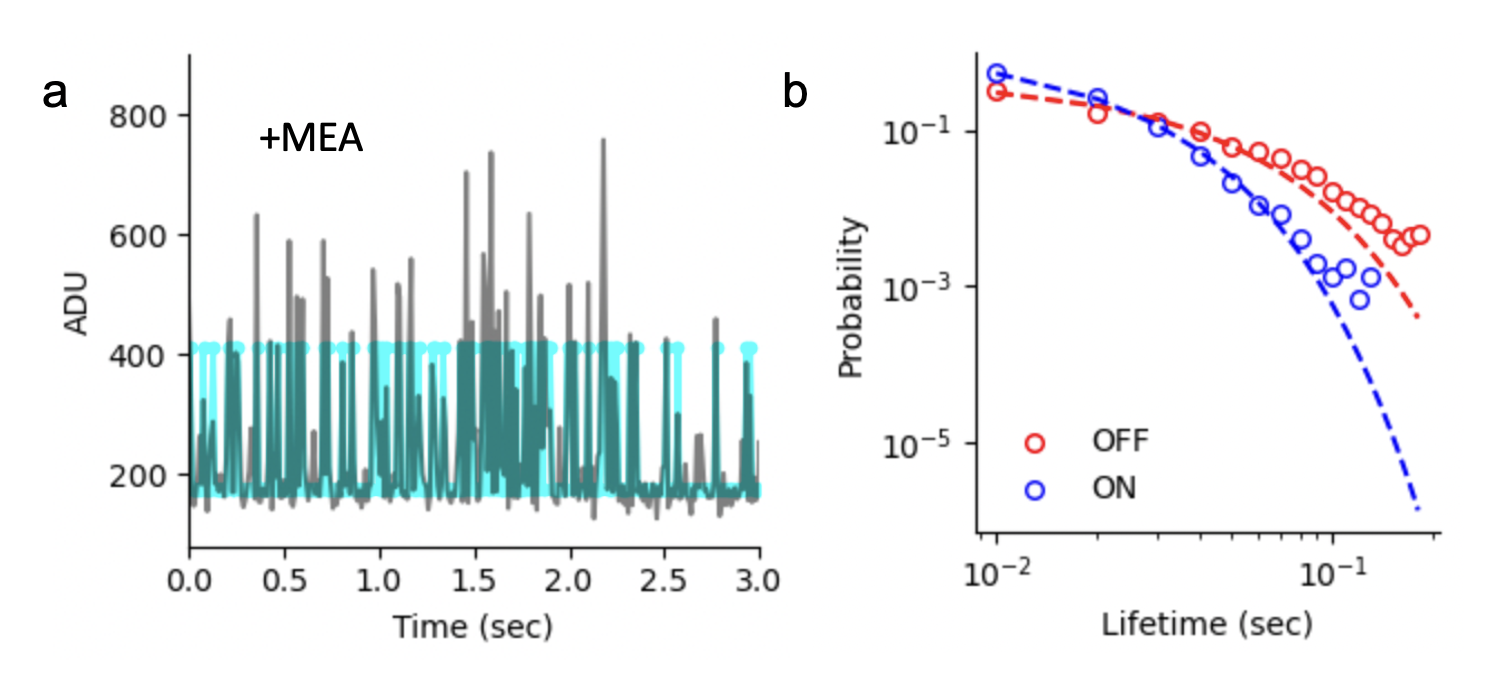
\includegraphics[width=13cm]{media/Lifetime.png}
\caption{\textbf{Photoswitching of JF646 bound to H2B-HaloTag} (a) Peak intensity fluctuations of a putatively isolated JF646 molecule exicted at 640nm and imaged with 10ms exposure time in the presence of 100mM MEA buffer. Fit of a Hidden Markov Model is shown in cyan (b) ON and OFF state lifetime distributions found by pooling data from 16 JF646 spots in a single HeLa cell nucleus. Single component exponential fits shown as dashed lines.}
\label{fig:fig16}
\end{figure}


Super-resolved nucleosome organization has been studied extensively in fixed cells to reveal segregated
nanodomains hundreds of nanometers in size, including dispersed nanodomains and compact large aggregates. Nucleosomes are now known to assemble into heterogeneous clusters of variable sizes, interspersed with nucleosome-depleted regions \parencite{Ricci2015}. However, our current understanding of nucleosome patterning in the nucleus is limited by the need for fixation. Chemical fixation with paraformaldehyde, glutaraldehyde, methanol, or other chemical fixatives may alter the structure of chromatin, introducing error in our measurements \parencite{Maeshima2020}. Live cell imaging carries its own issues, particularly due to local and long-range chromatin motions in the nucleus. At the nanoscale, local chromatin motion appears to be isotropic and driven by thermal fluctuation \parencite{Maeshima2020}. Therefore, we presume that for sufficiently brief imaging duration (tens of seconds) nanodomain structure is approximately static. As a consequence, vibrations of single nucleosomes are, in effect, an addition of low amplitude noise to the localization dataset. 

To perform live cell super-resolution imaging of chromatin nanodomains, we adopt the HaloTag system, a modified haloalkane dehalogenase designed to covalently bind to synthetic ligands (Los 2008). The HaloTag protein is fused to nucleosome H2B and is then bound by a rhodomine-derived fluorescent ligand, JF646. JF646 undergoes fluorescence intermittency (blinking) in the presence of a cysteamine (MEA) containing buffer (Figure \ref{fig:fig16}). Once precise positions of the fluorophores are obtained, Besag’s L-function $L(r)$ is used to analyze the clustering. The L-function $L(r)= \sqrt{\frac{K(r)}{\pi}}$ is a transformation of Ripley’s K-function $K(r)$. The function $K(r)$ is designed such that $K(r)$ is the number of localizations within a radius $r$ of a randomly chosen localization. Importantly, in the case of complete spatial randomness, $L(r)=r$. Thus, in general, to quantify the degree of clustering, one uses $L(r)-r$, which measures the deviation of a point pattern from CSR. To demonstrate this, example point patterns have been generated using complete spatial randomness (Figure \ref{fig:fig17}) or a Thomas point process (Figure \ref{fig:fig18}). Note that $\sigma=0$ is used to denote CSR. The Thomas process is parameterized by the standard deviation of a point from its cluster center $\sigma$. under CSR  and a Thomas point process. 


\begin{figure}
\centering
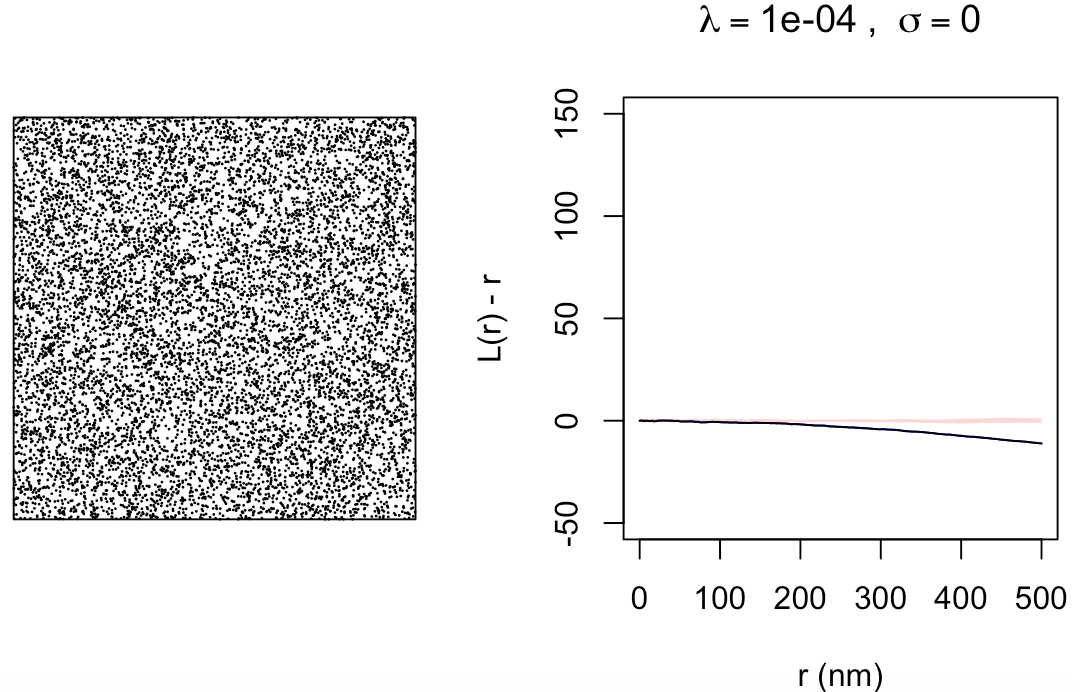
\includegraphics[width=10cm]{/Users/cwseitz/git/cwseitz.github.io/docs/phd/brd4/brd4/media/ppp/csr-1e4-0.png}
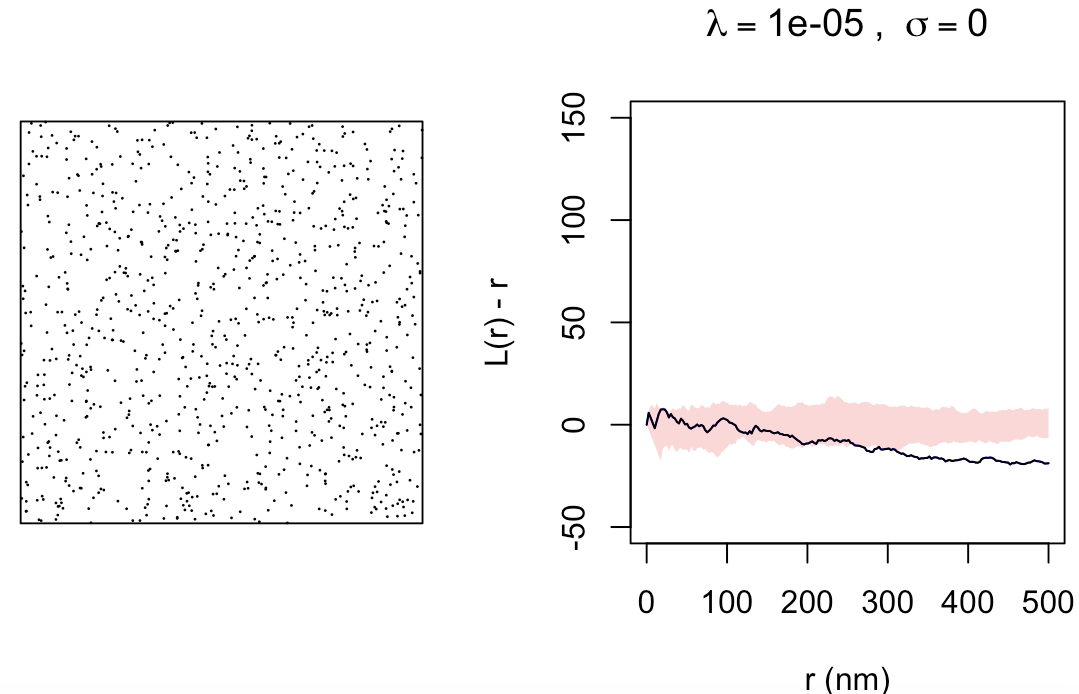
\includegraphics[width=10cm]{/Users/cwseitz/git/cwseitz.github.io/docs/phd/brd4/brd4/media/ppp/csr-1e5-0.png}
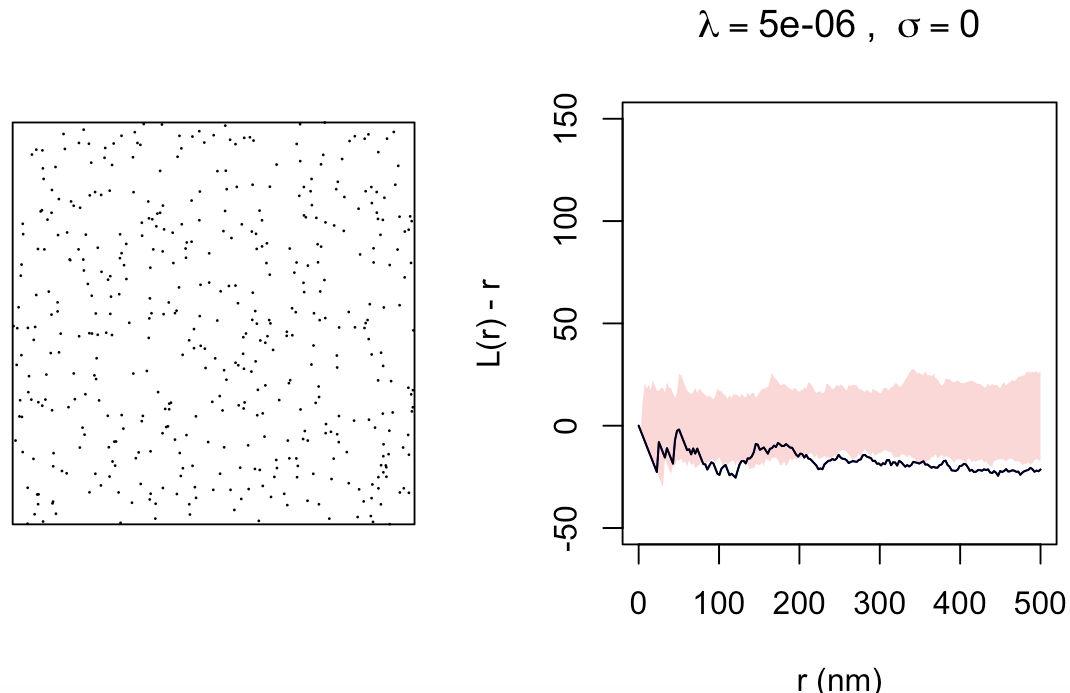
\includegraphics[width=10cm]{/Users/cwseitz/git/cwseitz.github.io/docs/phd/brd4/brd4/media/ppp/csr-5e6-0.png}
\caption{\textbf{Besag's L-function under complete spatial randomness (CSR)} Point pattern simulations for CSR for various intensities of the point process. Simulation envelopes are shown in pink, which represent the significance band of the estimated $L(r)-r$}
\label{fig:fig17}
\end{figure}

\begin{figure}
\centering
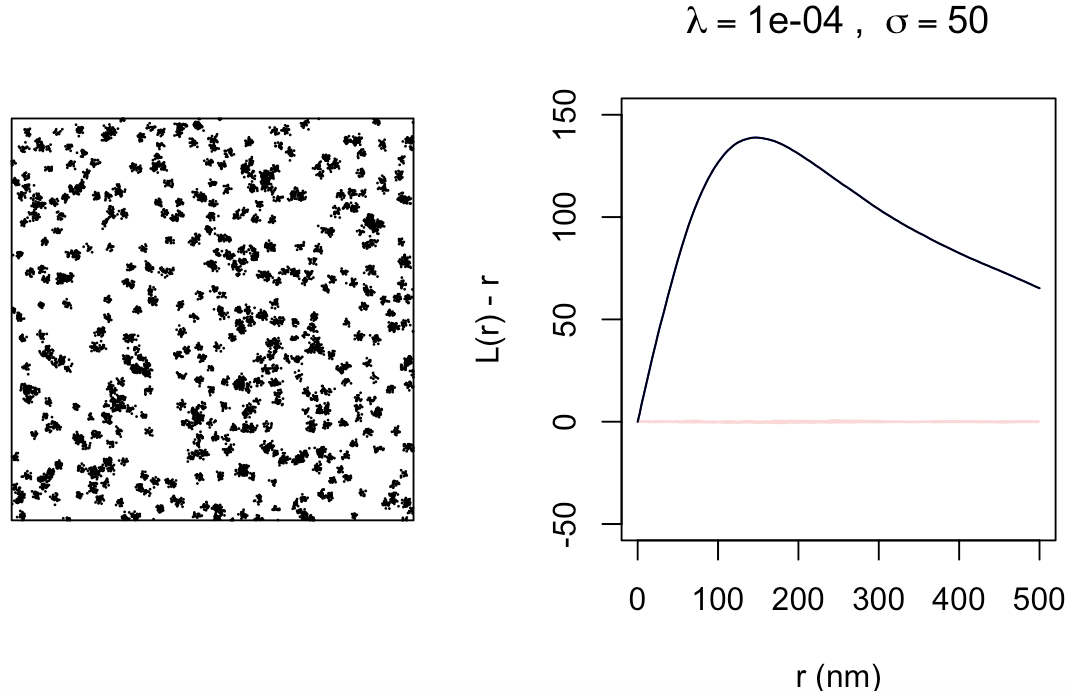
\includegraphics[width=10cm]{/Users/cwseitz/git/cwseitz.github.io/docs/phd/brd4/brd4/media/ppp/tom-1e4-50.png}
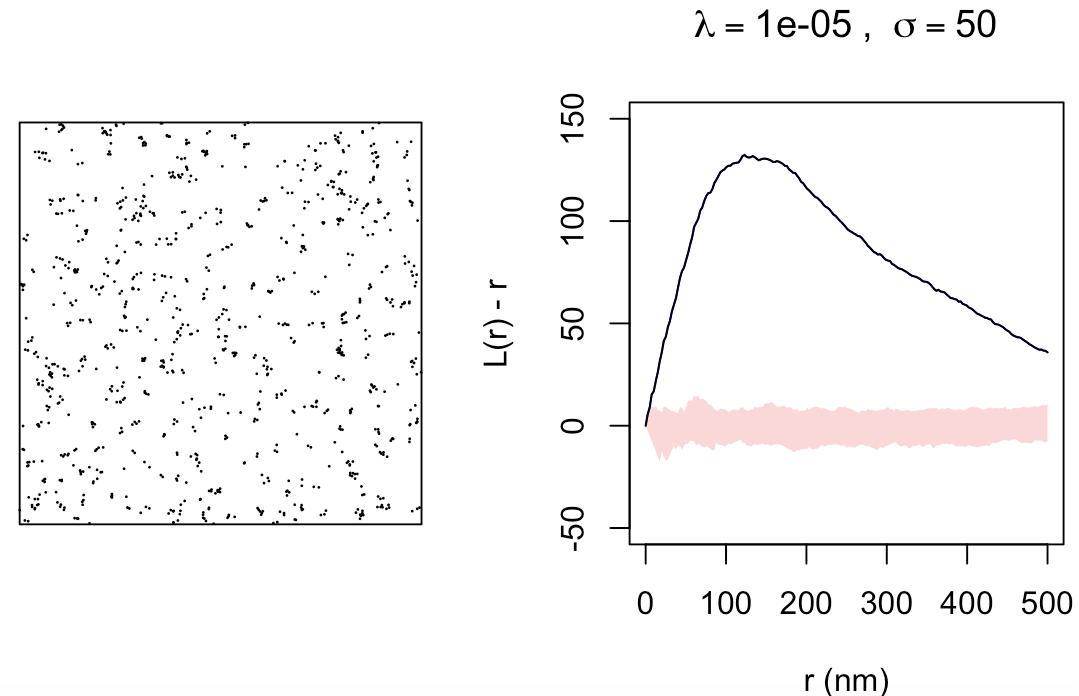
\includegraphics[width=10cm]{/Users/cwseitz/git/cwseitz.github.io/docs/phd/brd4/brd4/media/ppp/tom-1e5-50.png}
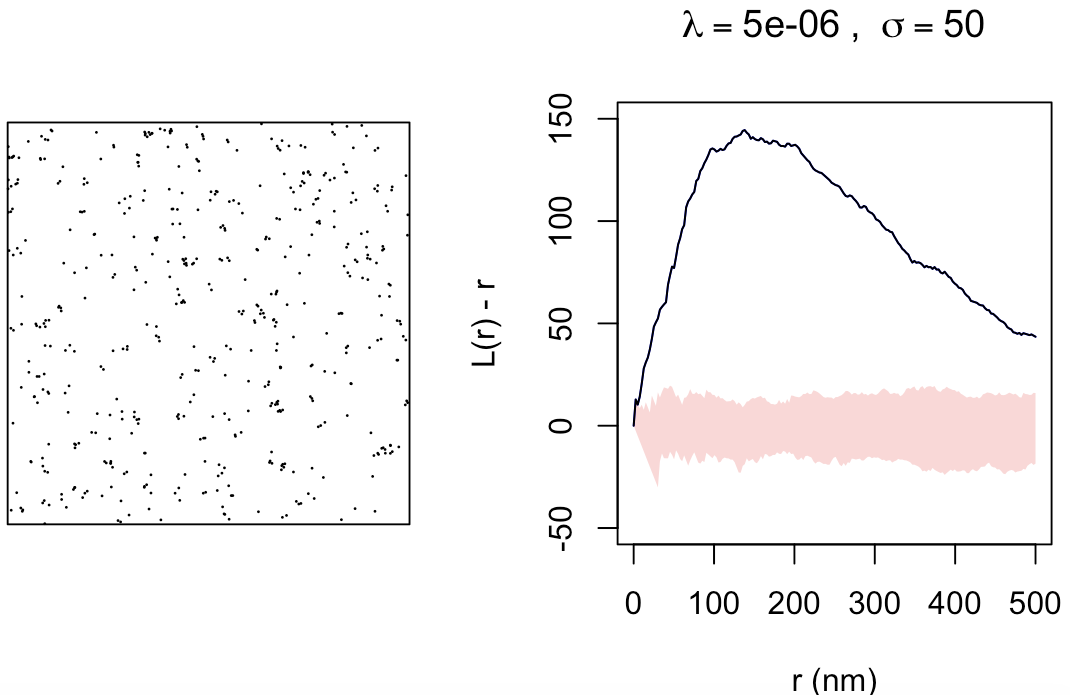
\includegraphics[width=10cm]{/Users/cwseitz/git/cwseitz.github.io/docs/phd/brd4/brd4/media/ppp/tom-5e6-50.png}
\caption{\textbf{Besag's L-function for a Thomas process} Point pattern simulations for the Thomas process ($\sigma=50\mathrm{nm}$) for various intensities of the point process. Simulation envelopes are shown in pink, which represent the significance band of the estimated $L(r)-r$}
\label{fig:fig18}
\end{figure}
\clearpage


\section{Polymer models and chromatin dynamics}

By accumulating single molecule localizations over a time series of frames, quantitative information regarding the motion of the particle can be extracted and related to experimental conditions. It is important to note that the chromatin structure is highly complex and cannot be exactly represented by the diffusion of individual particles. However, by treating each fluorescent spot as a point mapped in space and time, we can extract parameters of the diffusion and classify tracks as sub-diffusive, Brownian, or super diffusive. 

The well-known diffusion equation is a special case of the more general Kramers-Moyal expansion, which describes the dynamics of the probability density of a stochastic process $P(x,t)$ \parencite{Gardiner2009}. Pure diffusion is the case where transitions in the process are drawn from a distribution with zero mean (zero drift) and constant variance. 

\begin{equation}
\frac{\partial P(x,t)}{\partial t}  = D\frac{\partial^{2}P(x,t)}{\partial x^{2}}
\end{equation}

The diffusion coefficient $D$ is in fact just half of the variance of the transition distribution $D = \sigma^{2}/2$. We would like to solve the above equation, but it is a PDE which usually require some tricks to solve e.g., integral transforms. This particular PDE can be solved by Fourier transformation. For brevity, I simply state the result

\begin{equation}
P(x,t) = \frac{1}{\sqrt{2Dt}}\exp\left(- \frac{(x-x_{0})^{2}}{4Dt}\right)
\end{equation}

which is a Gaussian distribution will time-dependent variance $\sigma=4Dt$, given originally by Einstein in his famous paper on Brownian motion in 1905. The most common method to analyze single particle trajectories is to calculate the mean square displacement (MSD), which can be used to determine the diffusion coefficient $D$.

\begin{equation}
\text{MSD} = \frac{1}{N} \sum_{i=1}^{N} \left[ \mathbf{r}(t + \tau) - \mathbf{r}(t) \right]^2
\end{equation}

The sampling time given by $\tau$ is interpreted as the frame rate of the camera. Certain studies have shown that the observed motion varies with different values of $\tau$ \parencite{Amitai2017,Shukron2017}. It is not difficult to see that the solution to the diffusion equation has a MSD which is linear: $\text{MSD}(\tau) = 4Dt$. A linear MSD is therefore a defining characteristic of Brownian motion. Sub-diffusive and super-diffusive diffusion can be classified by use of the more general anamalous diffusion model:

\begin{equation}
\text{MSD}(\tau) = 2mD\tau^\alpha
\end{equation}

where $m$ is the number of dimensions. For trajectories with $\alpha = 1$, the motion is considered to be Brownian motion; when $\alpha > 1$, it is said to be superdiffusive; and $\alpha < 1$ is classified as subdiffusive. Importantly, different parameter values allow for further interpretation and classification of different diffusion modes of particles \parencite{Wasim2018,Zhong2020}.

By comparing the $D$ values of all particles within the nucleus, spatial heterogeneity can be clarified. While the calculation of $D$ and $\alpha$ is particularly reliant on the length of the trajectory and the number of data points, recent investigations have built diffusion color maps of fluorescently labeled histones by computing vast amounts of super-resolution trajectories \parencite{Amitai2017,Barth2020,Nozaki2017}.

\subsection{Trajectory linking}

A diverse set of particle tracking algorithms utilize probabilistic models of particle motion in order to add detected particles to existing tracks. Perhaps the most fundamental particle tracking method in this category is the nearest neighbor linking algorithm first introduced by Crocker and Grier \parencite{Crocker1996}. The algorithm constructs particle trajectories by assuming that the ensemble consists of non-interacting indistinguishable particles undergoing Brownian motion. As a result, the displacement of each particle follows a Gaussian distribution, parameterized by the diffusion coefficient and the time-resolution of the sequence. The most probable assignment of detected particles to existing tracks can then be found by maximizing the product of several Gaussian distributions \parencite{Crocker1996}. An attractive feature of this algorithm is that it is relatively simple to implement; however, assumptions that underlie the method impose limitations. In particular, if a typical displacement $\delta$ in one time step is comparable to the typical inter-particle spacing, tracking becomes highly error-prone \parencite{Crocker1996}. In other words, when particles are simultaneously densely distributed and undergoing fast diffusion, the algorithm can fail to build accurate trajectories due to the ambiguity introduced by overlapping trajectories. This also applies to the limit of low frame rates when small displacements are not recorded by the sensor. Importantly, the method alone cannot handle cases where particles disappear permanently, temporarily disappear due to blinking, photo-bleaching, or missed localization \parencite{Sbalzarini2005}.

\subsection{Chromatin polymer models}

\begin{figure}[t]
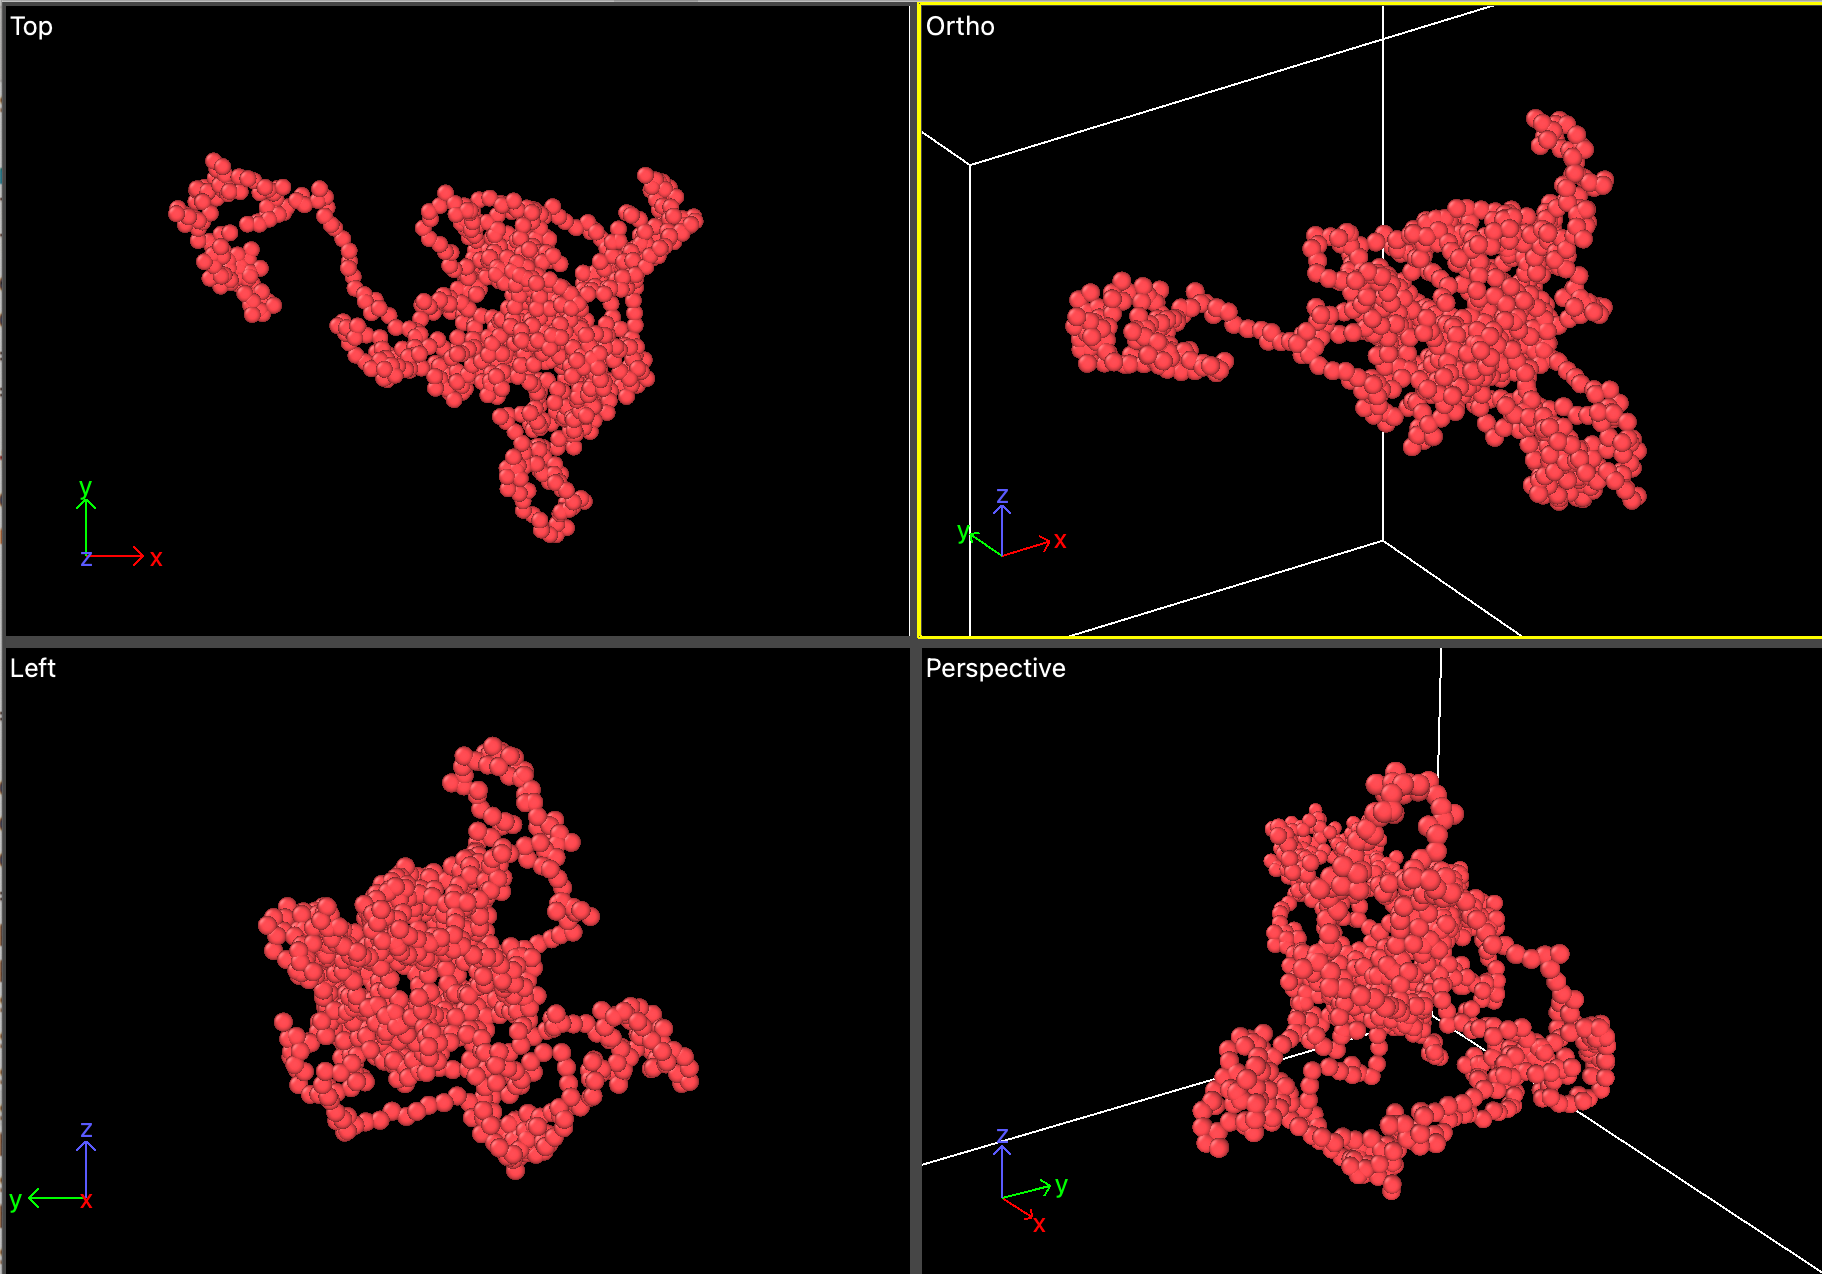
\includegraphics[width=\textwidth]{/Users/cwseitz/git/cwseitz.github.io/docs/phd/brd4/brd4/media/Rouse.png}
\caption{\textbf{Snapshots of the Rouse polymer} Four perspectives of the Rouse polymer generated with $N=2000$ beads connected with harmonic bonds with equilibrium length $200\mathrm{nm}$. Polymer is initialized with all harmonic bonds at equilibrium}
\label{fig:fig19}
\end{figure}


It is well-known that the DNA double helix structure consists of millions of base pairs chained together by the sugar-phosphate backbone. DNA, being a molecule built from many similar monomers bonded together, is naturally analyzed using a polymer model. The simplest polymer model for chromatin is the Rouse polymer model, which utilizes monomers connected by springs, resembling the string-of-beads structure observed under the electron microscope (Figure \ref{fig:fig19}). Forces acting on a bead by neighboring beads results in confinement and subdiffusive dynamics (Figure \ref{fig:fig20}). To refine the modeling of chromatin properties according to the exponent $\alpha$, the $\beta$-polymer model was introduced. This model accounts for mid-range and long-range interactions between monomers. Indeed, the $\beta$-polymer model can be selected to address cases where $\alpha$ is in the range of 0 to 0.5 \parencite{Amitai2013,Amitai2017,Hajjoul2013}.


\begin{figure}[t]
\centering
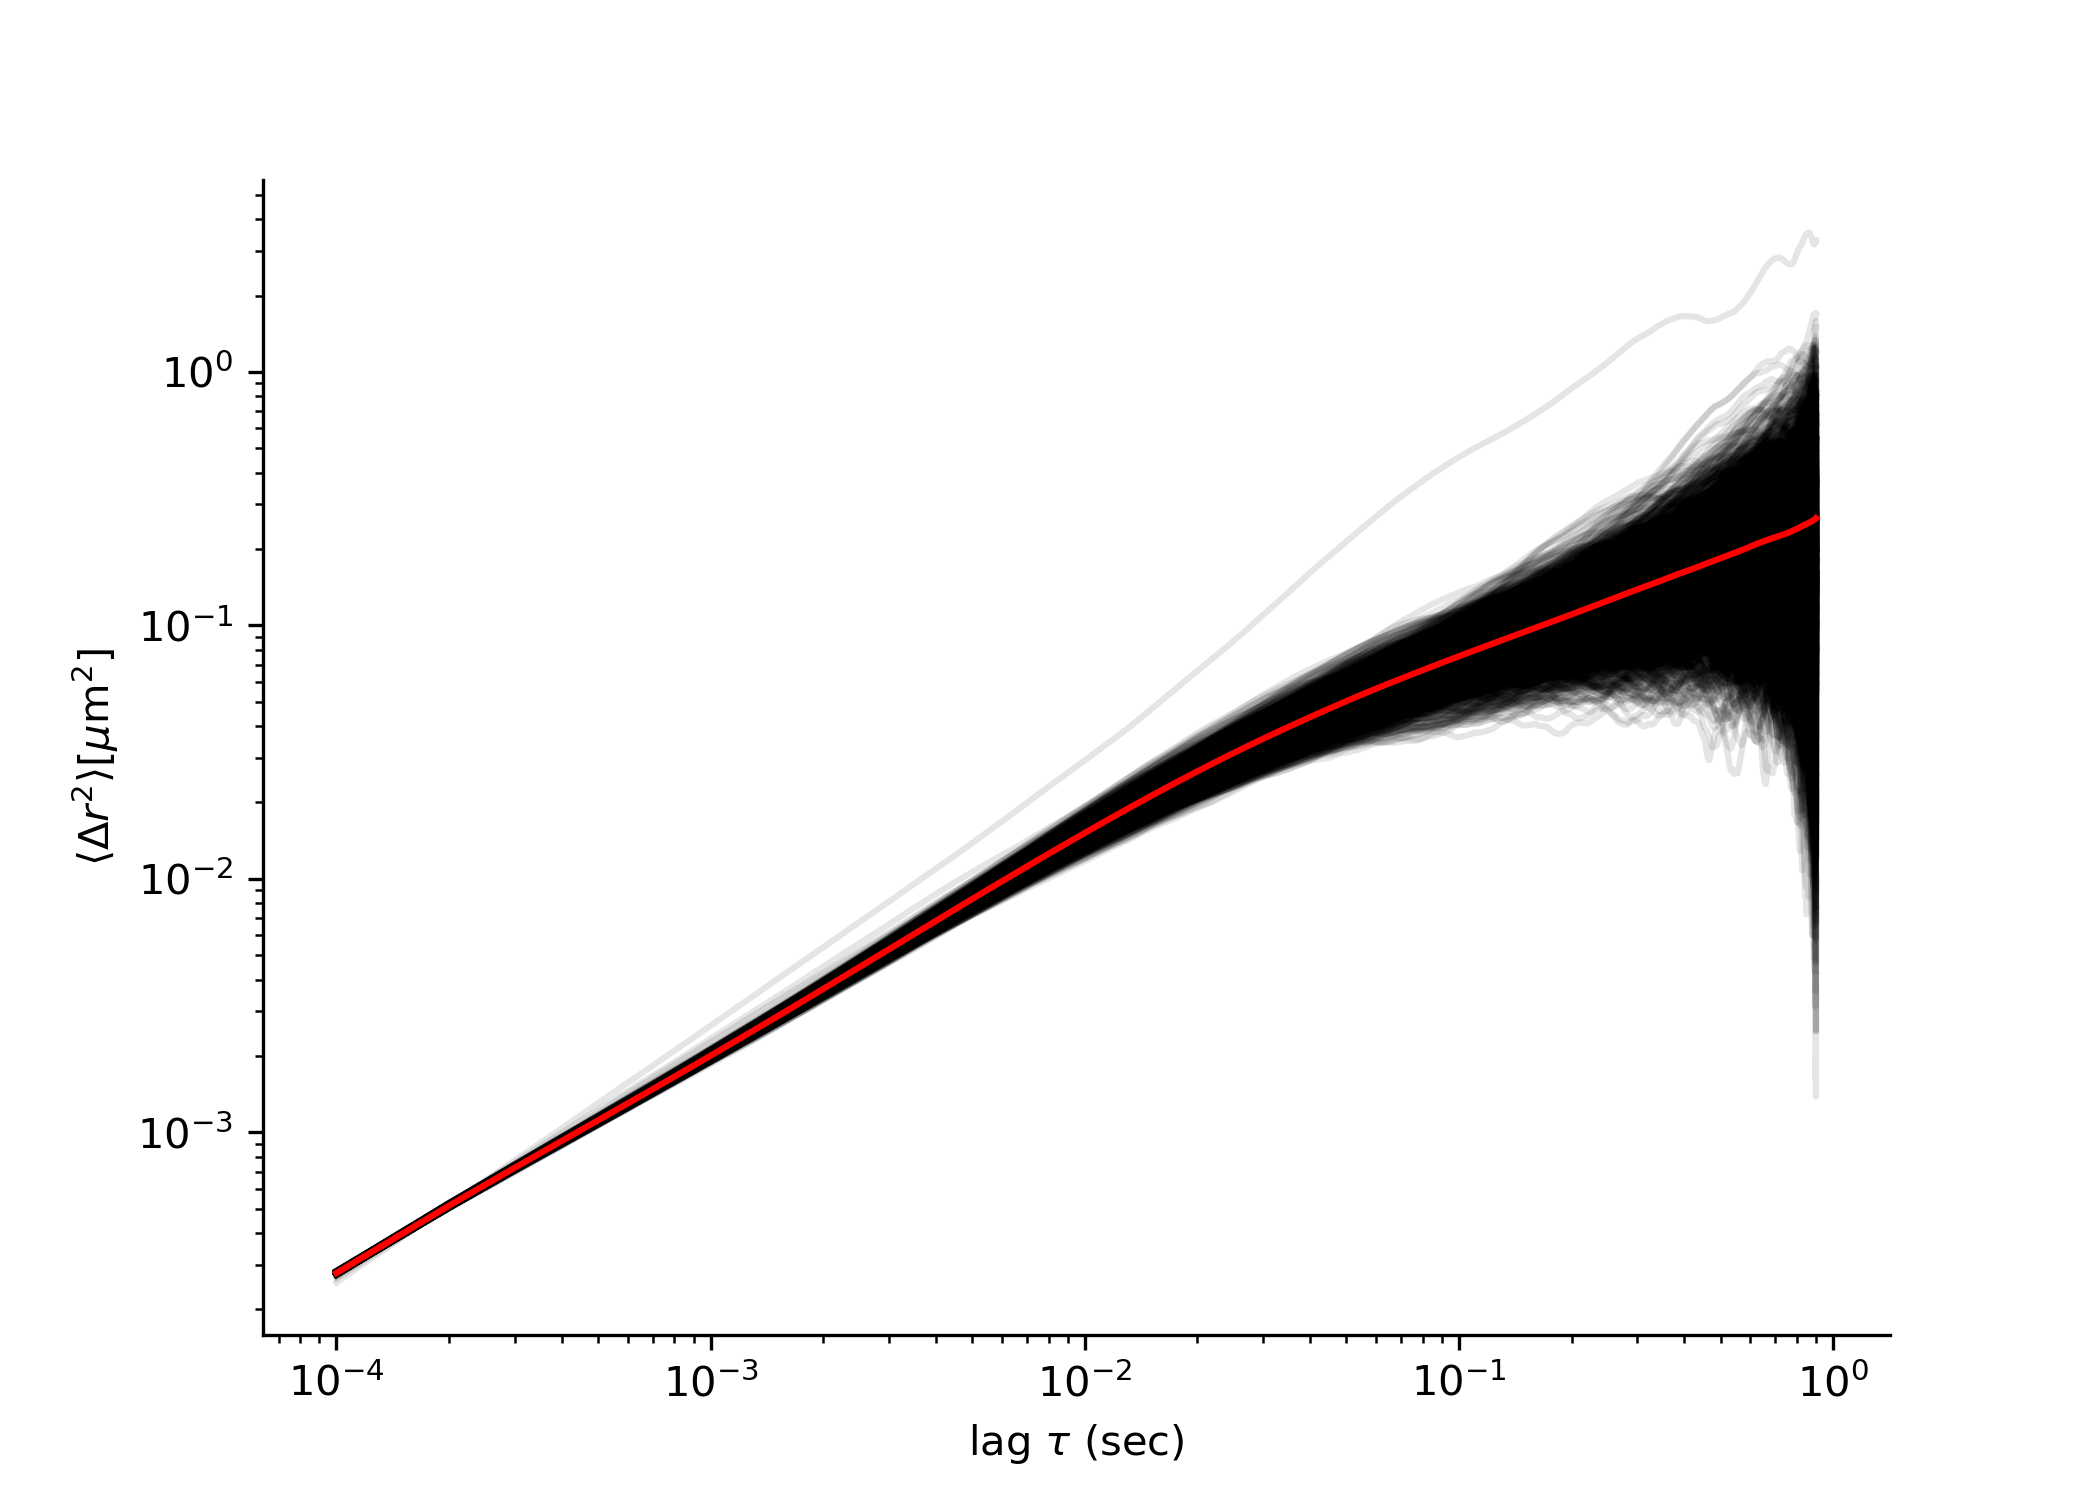
\includegraphics[width=13cm]{/Users/cwseitz/git/cwseitz.github.io/docs/phd/brd4/brd4/media/Rouse-Dynamics-1.png}
\caption{\textbf{Subdiffusive dynamics of a Rouse polymer} Mean squared displacement (MSD) of 2k beads shown in black, average MSD shown in red.}
\label{fig:fig20}
\end{figure}


\begin{table}[h!]
\centering
\begin{tabular}{|c|c|}
\hline
\textbf{Parameter} & \textbf{Value} \\ \hline
Temperature ($T$) & 310 K \\ \hline
Bond Length ($\sigma$) & $200 \times 10^{-9}$ m \\ \hline
Cutoff Distance & $500 \times 10^{-9}$ m \\ \hline
Spring Constant ($\kappa$) & 90.0 $k_{B}T/\sigma^2$ \\ \hline
Neighbor Distance & $500 \times 10^{-9}$ m \\ \hline
Damping Coefficient ($\gamma$) & $10^{-4}$ \\ \hline
Time Step & 1s\\ \hline
Number of Time Steps & $10^4$ \\ \hline
Number of Atoms & 2000 \\ \hline
\end{tabular}
\caption{\textbf{Rouse polymer parameters}}
\end{table}

%\begin{figure}[th]
%\centering
%\includegraphics[width=13cm]{/Users/cwseitz/git/cwseitz.github.io/docs/phd/brd4/brd4/media/Rouse-%Dynamics-2.png}
%\caption{\textbf{Subdiffusive dynamics of the Rouse polymer}. (left) Histogram of the diffusion %coefficient of individual beads. (right) Histogram of the anamalous exponent. Fitting of %individual bead MSDs performed by linear regression in log-space using the first 5000 time points}
%\label{fig:fig21}
%\end{figure}

Furthermore, as the polymer model usually folds at different spatial scales and generates various sizes of loops, a simulation model adding connectors between randomly chosen non-nearest neighbor monomer pairs, known as the randomly cross-linked (RCL) polymer model, was presented. In this model, $\alpha$ is reduced to below 0.5 by adding connectors. Recent evidence suggests that the number and distribution of connectors impact physical parameters in various ways, but this domain remains underexplored. Notably, the RCL polymer model may be crucial for studying dynamics in processes such as CTCF and cohesion regulating chromatin loop stability \parencite{Hansen2017}.

\clearpage
\section{BRD4 phosphorylation regulates the structure of chromatin nanodomains}

The cell nucleus is a densely packed environment with chromatin comprising a dominant component. The compartmentalization of chromatin with other intranuclear components by phase separation is therefore an efficient strategy to ensure precise spatial and temporal coordination of complex dynamics. A growing number of phase separated nuclear bodies have been identified, including transcriptional condensates \parencite{Sabari2018,Hnisz2017}, nuclear speckles \parencite{Brown2008}, and DNA damage repair foci \parencite{Wang2023}; however, the interplay of phase separated condensates with the underlying chromatin structure remains poorly understood. Transcriptional condensates have been identified as an ideal model to study the kinetic and thermodynamic contributions of chromatin substrate binding, as the ability of transcriptional activators to both condense and bind chromatin is well established \parencite{Sabari2018,Wagh2021,Plys2018,Strom2024,Ma2021}. Here, we extend this effort by investigating the regulation of chromatin structure by phase separated transcriptional condensates. We focus on the BRD4 protein - a well-studied transcriptional activator that localizes to acetylated chromatin sites \parencite{Wu2018}, recruits pTEF-b, and initiates transcription of key genes involved in signal response, immunity, and oncogenesis \parencite{Itzen2014}.

The BRD4 long isoform is characterized by structured N-terminal tandem acetyl-lysine binding bromodomains and an extra-terminal domain, connected by intrinsically disordered regions \parencite{Han2020}. Perhaps the most fundamental of BRD4 functions is the ability to bind to acetylated chromatin through bromodomain 1 (BD1) and bromodomain 2 (BD2) that are in tandem within the N-terminal part of the protein (Figure \ref{fig:fig22}). BRD4 inhibitors such as (+)-JQ1 competitively bind to the acetyl-binding pocket of BRD4, displacing BRD4 from chromatin \parencite{Filippakopoulos2010}. It is also well known that BRD4 association with acetylated chromatin is enhanced by casein kinase II (CK2)-mediated phosphorylation of seven N-terminus phosphorylation sites (NPS), followed by intramolecular rearrangement of BRD4 protein and/or BRD4 dimerization \parencite{Wu2013,Malvezzi2021}.

\begin{figure}[t]
\centering
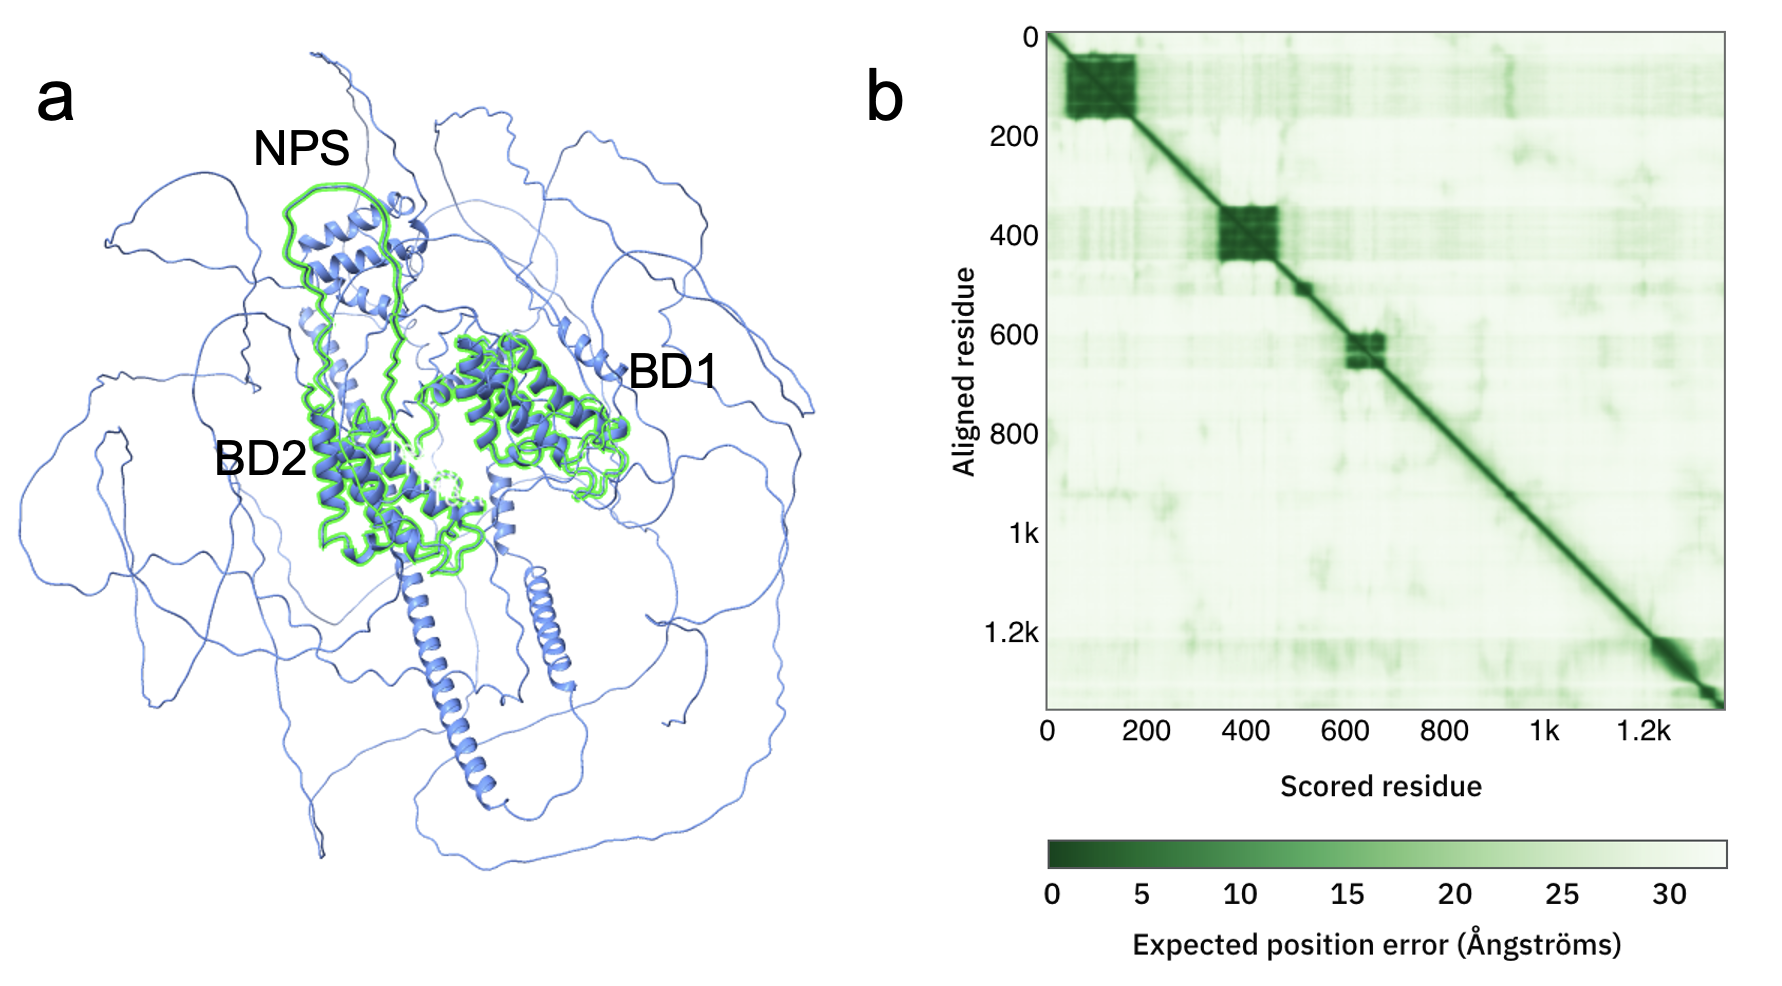
\includegraphics[width=14cm]{/Users/cwseitz/git/cwseitz.github.io/docs/phd/brd4/brd4/media/Structure.png}
\caption{\textbf{Bromodomain protein 4 (BRD4) structure prediction} (a) AlphaFold predicted structure of BRD4 long isoform (blue) with bromodomain 1 (BD1) aa58-163, bromodomain 2 (BD2) aa349-456, and N-terminus phosphorylation sites (NPS) aa462-506 highlighted in green (b) Heat map of expected position error in AlphaFold prediction}
\label{fig:fig22}
\end{figure}

Recent studies have demonstrated that BRD4 is present in discrete nuclear bodies that occur at super-enhancers, which exhibit properties of other well-studied biomolecular condensates, including rapid recovery of fluorescence after photobleaching and sensitivity to 1,6-hexanediol, which disrupts liquid-like condensates \parencite{Sabari2018}. Both BRD4 long and short isoform are found in phase separated condensates in the nucleus and are associated with active gene transcription. Importantly, CK2-mediated NPS phosphorylation state regulates chromatin binding activity of BRD4 as well as BRD4 phase separation \parencite{Han2020}. This has led to the conclusion that phosphorylation of BRD4 inhibits interaction with chromatin and reduces phase separation, while remaining necessary for active gene transcription. Moreover, phosphorylated and unphosphorylated BRD4 form different molecular associations – transient polyvalent associations of unphosphorylated BRD4 contrast with the stable dimeric interaction and chromatin binding of phosphorylated BRD4 \parencite{Malvezzi2021}. Therefore, we speculated that BRD4 phosphorylation can modulate a multivalent binding interaction between the transcriptional condensate with NNs, making BRD4 phosphorylation necessary for the maintenance of NN structure and dynamics.


\subsection{Results}

\subsubsection{Colocalization of BRD4 mutants with nucleosome nanodomains}

To address the role of BRD4 binding and phase separation on chromatin structure, we express FLAG-tagged BRD4 mutants with NPS or bromodomain mutations in HeLa cells and measure their effects on chromatin organization. In particular, we express a constitutively phosphorylated (7D mutant), constitutively unphosphorylated (7A mutant), and bromodomain-deactivated (BD mutant) protein (Figure \ref{fig:fig23} a,b,c). Colocalization analysis of BRD4 mutants with NNs using nearest neighbor distance distribution showed an obvious colocalization of these mutants with NNs. The 7D mutant showed the closest proximity to NNs relative to wild type, followed by BD and 7A mutants (Figure \ref{fig:fig23} d).  This result is consistent with known dependence of BRD4 chromatin binding on phosphorylation state. 

\begin{figure}[t]
\includegraphics[width=\textwidth]{/Users/cwseitz/git/cwseitz.github.io/docs/phd/brd4/brd4/media/Figure-0.png}
\caption{\textbf{BRD4 mutants colocalize with nucleosome nanodomains} (a) Schematic of the BRD4 protein sequence and mutations shown in red. (b) Anti-FLAG western blot of bulk expression of BRD4 mutants (c) Combined immunofluorescence of FLAG-tagged BRD4 mutants with JF646-tagged H2B-Halo (d) Histograms of nearest neighbor distances of H2B puncta to FLAG puncta over 10 cells for each mutant. Red dashed lines are drawn at the mean, statistical significance determined by Welch t-test for each mutant relative to wild-type (WT) * p<0.05, *** p<0.001}
\label{fig:fig23}
\end{figure}
	
\subsubsection{BRD4 condensates regulate chromatin structure and dynamics}

To assess the functional role of BRD4 in maintaining the NN environment, we interrogated the dynamics of NNs, as well as their structure, in the presence of BRD4 mutants. Histone H2B was tagged with HaloTag \parencite{Los2008} (H2B-Halo), to which a fluorescent ligand JaneliaFluor646 (JF646) can bind specifically in a living cell. Low concentrations of JF646 were used to obtain sparse labeling of nucleosomes for single-nucleosome imaging (Figure \ref{fig:fig26} a,b). JF646-labeled nucleosomes in HeLa cells were recorded at 10fps (∼200 frames, 20 s total) and a reduced diffusion coefficient was measured in cells expressing 7A, 7D, and BD mutants, with respect to cells expressing the wild-type BRD4 protein (Figure \ref{fig:fig26} c). HeLa cells exposed to (+)-JQ1 in DMSO for 8h showed an increase in nucleosome dynamics with respect to DMSO alone (Figure \ref{fig:fig26} d). We then conducted super resolution imaging of NN using direct stochastic optical reconstruction microscopy (dSTORM) by promoting JF646 fluorescence intermittency with a cysteamine buffer (Figure \ref{fig:fig25} a,b). JF646 is known to exhibit a transient fluorescent state lasting tens to hundreds of milliseconds and stable dark state lasting hundreds of milliseconds to seconds \parencite{Grimm2015}. Two color imaging of H2B-Halo-JF646 and GFP-tagged BRD4 shows that BRD4 and NNs form complementary biomolecular condensates in the nucleus, consistent with current models of BRD4 chromatin reading mechanism (Figure \ref{fig:fig25} c). Ensemble averages of Besag’s L-function showed an increase in nucleosome clustering in cells expressing the 7D BRD4 mutants, while all other groups were consistently indistinguishable from WT cells (Figure \ref{fig:fig25} e). HeLa cells exposed to (+)-JQ1 in DMSO for 8h showed a reduction in nucleosome clustering with respect to DMSO alone (Figure \ref{fig:fig25} f).  

\begin{figure}[t]
\includegraphics[width=\textwidth]{/Users/cwseitz/git/cwseitz.github.io/docs/phd/brd4/brd4/media/Figure-1.png}
\caption{\textbf{Strong multivalent chromatin binders reduce diffusion of nucleosome nanodomains} (a) Heteropolymer model of chromatin consisting of A-type, B-type, and C-type particles (b) Interaction potentials $U_{BC}(r_{ij})$ of multivalent chromatin binders with B-type chromatin beads (c,d) Example free heteropolymer and heteropolymer with a number density of C-type particles of $\rho=500/\mu m^3$ in a 10um periodic box (e) Scaled diffusion coefficient $D$ for various chromatin binding energies of C-type particles, averaged over ten independent simulations, with burn-in discarded.}
\label{fig:fig24}
\end{figure}

\begin{figure}[t]
\includegraphics[width=\textwidth]{/Users/cwseitz/git/cwseitz.github.io/docs/phd/brd4/brd4/media/Figure-2.png}
\caption{\textbf{Expression of constitutively phosphorylated BRD4 compacts nucleosome nanodomains} (a,b) Direct stochastic optical reconstruction microscopy (dSTORM) imaging strategy of single nucleosomes and an example super-resolution image (c) Two-color image of super-resolved H2B-JF646 with diffraction-limited GFP-tagged BRD4 (d) Quantification of degree of clustering using the L-function (e) L-function for BRD4 mutants (f) L-function after 8h exposure to 1uM (+)-JQ1 in DMSO and DMSO only. All scalebars 3um. ** p<0.01, *** p<0.001}
\label{fig:fig25}
\end{figure}

\subsubsection{Heteropolymer model}

To interpret our experimental findings, we adopt a heteropolymer chromatin model to capture the interaction of chromatin with multivalent BRD4-like binders (Figure \ref{fig:fig24} a). The heteropolymer consists of a coarse-grained bead-and-spring chain composed of $N_b=200$ beads, connected by harmonic bonds with equilibrium length $r_0$ whose energy is defined as

\begin{equation}
U_{AB}(r_{ij})=\frac{\kappa}{2}(\lvert r_{ij}\lvert-r_0)^2
\end{equation}

where $r_{ij}$ is a vector connecting the center of a bead of type $i$ to a bead of type $j$ and $i,j \in (A,B)$. In all simulations, we assume $\kappa=90k_{B}T{r_0}^2$ where $k_{B}$ is the Boltzmann constant and $r_0=200$nm. Random beads in the chain are selected to represent locally unacetylated (A-type particles) and acetylated chromatin (B-type particles).  B-type particles undergo multivalent interactions with a third group of C-type particles, which can promote cross-linking of the polymer. We presume a Bernoulli probably of $p=0.3$ for any given bead to be in an acetylated-like state. Interaction of multivalent chromatin binders with chromatin beads are then mediated by the following potential:

\begin{equation}
U_{BC}\left(r_{ij}\right)=\epsilon\left(1-\left(\frac{\lvert r_{ij}\lvert}{R_0}\right)^2\right)^3
\end{equation}

where $R_0=200$nm. The potential $U_{BC}$ is considered over a domain $0\leq\lvert r_{ij}\lvert\leq 2 R_0$ In all simulations, ten replicates were run for each condition tested. A and B type particles within the chromatin polymer have repulsive interactions with $\epsilon = +10k_{B}T$. Binding energy of the acetylated beads with binders was varied with $\epsilon_{I} = 0 k_{B}T,\epsilon_{II} = -20k_{B}T,\epsilon_{III}=-40k_{B}T$ (Figure \ref{fig:fig24} a). The dynamics of chromatin chains are approximated by Brownian dynamics within a cubic box with side length of 10um and periodic boundary conditions. Brownian dynamics follows the stochastic differential equation.

\begin{figure}[t]
\includegraphics[width=\textwidth]{/Users/cwseitz/git/cwseitz.github.io/docs/phd/brd4/brd4/media/Figure-3.png}
\caption{\textbf{BRD4 mutants reduce single nucleosome dynamics in living cells} (a,b) Sparse labeling of single nucleosomes in a living HeLa cell (scalebar 5um) (c) Average mean squared displacement (MSD) of single nucleosomes for wild-type and mutated BRD4, error bars represent the standard error of the mean (d) Average MSD of single nucleosomes after 8h exposure to 1uM (+)-JQ1 in DMSO and DMSO only, error bars represent the standard error of the mean}
\label{fig:fig26}
\end{figure}

\begin{table}[h!]
\centering
\begin{tabular}{|c|c|}
\hline
\textbf{Parameter} & \textbf{Value} \\ \hline
Bond Length ($\sigma$) & $200 \times 10^{-9}$ m \\ \hline
Cutoff Distance & $500 \times 10^{-9}$ m \\ \hline
Spring Constant ($\kappa$) & 90.0 $k_{B}T/\sigma^2$ \\ \hline
Neighbor Distance & $500 \times 10^{-9}$ m \\ \hline
Damping Coefficient ($\gamma$) & $10^{-7}$ \\ \hline
Time Step & $10^{-4}$s\\ \hline
Number of Time Steps & $10^4$ \\ \hline
Number of Atoms & 200 \\ \hline
\end{tabular}
\caption{\textbf{Multivalent binder model parameters}}
\end{table}

\begin{equation}
\dot{\bold{r}} = \gamma^{-1}\nabla U(\bold{r}) +\sqrt{2 k_{B}T}\gamma^{-1/2}\xi(t)
\end{equation}

where $\gamma$ is a diagonal friction tensor and $\xi(t)$ is a three-dimensional delta-correlated white noise $\langle \xi(t)\xi(t+\tau)  = \delta(t,t+\tau)$. Integrating the Brownian dynamics showed an overall reduction of the variance of the diffusion coefficient $D$ of single beads, and quasi-linear scaling of the diffusion coefficient with respect to temperature (Figure \ref{fig:fig24} e).

\subsection{Discussion}

Our data support the model that phosphorylated and unphosphorylated BRD4 form different molecular associations in the nucleus. BRD4 nuclear localization is only weakly affected by bromodomain inhibition with monovalent BET inhibitors, while exposure to phase separation inhibitors such as 1,6 Hexanediol have a significant effect on BRD4 localization in the nucleus. Colocalization activity of 7A/7D mutants relative to wild type measured here is consistent with this model of BRD4 localization to NNs. Strong colocalization of the BD mutant relative to the wild type suggests a possible link between bromodomain structure with localization of BRD4. 

Concurrently, reduced diffusivity of single nucleosomes with all mutants tested suggests a relationship between elevated colocalization and the degree of confinement of nanodomain diffusion. At the same time, increased nucleosome diffusivity and reduced nucleosome clustering after (+)-JQ1 exposure indicate BRD4 condensate formation is necessary in maintaining the nanodomain architecture. We further hypothesize effects of BRD4 localization on the viscosity of the nanodomain environment and potentially increased cross-linking of nanodomains. Indeed, we find this to be a natural result of molecular crowding resulting from overexpression of a constitutively phase separating protein, capable of multivalent interactions. Substantial colocalization of the 7D mutant with nanodomains along with increased chromatin compaction points towards a BRD4-mediated cross-linking mechanism of nucleosomes within the nanodomain. This result of increased affinity can also be seen in coarse grained simulations of chromatin interactions with multivalent binders.
 
We conclude that nascent BRD4 condensates are likely seeded by promiscuous interactions of BRD4 with cofactors, followed by phosphorylation followed by chromatin interactions mediated by the phosphorylated form. The stable dimeric interaction and binding of phosphorylated BRD4 to acetylated chromatin would then mediate control of the chromatin architecture by promoting cross-linking of the chromatin fiber and acting a molecular ‘bridge’ between transcriptional condensates with chromatin. 



\subsection{Materials and Methods}

\subsubsection{Cell lines, cell culture conditions, and transfection}

HeLa cells were cultured in DMEM supplemented with 10 percent fetal bovine serum (Gibco) at 37C 5 percent CO2 in a humidified incubator. Cultures were tested routinely for mycoplasma contamination; all tests were negative. For super-resolution experiments, cells were seeded in a 35mm FluoroDish (WPI), and transiently transfected using Lipofectamine 3000 with pBREBACK-H2BHalo plasmid (Addgene plasmid 91564) (ThermoFisher), pcDNA5-Flag-BRD4-7A (Addgene Plasmid 90006), pcDNA5-Flag-BRD4-7D (Addgene Plasmid 90007), pCDNA5-Flag-BRD4-BD (Addgene Plasmid 90005), pcDNA5-Flag-BRD4-WT (Addgene Plasmid 90331)

\subsection{Plasmid DNA purification}

Plasmids were transformed in E. coli at 4C and selected using an antibiotic agar plate. A single colony from the plate was selected and placed into sterile antibiotic LB Broth followed by incubation with shaking at 37C for 12h. After amplification, DNA was purified using a Miniprep kit (Promega). Following extraction, the concentration and purity were measured using the NanoDrop 2000 software. Plasmids were stored with optimal concentration and purity at -20C.

\subsubsection{Super-resolution imaging of nucleosome nanodomains in living cells}

After transient transfection, H2B-Halotag HeLa cells were incubated with 3pM JF646 HaloTag ligand overnight. Cells were imaged in a dSTORM photoswitching buffer containing 100mM MEA, 50 ug/ml Glucose Oxidase, and 3.4 mg/ml Catalase (Sigma). Buffer pH was adjusted to ~8 using HCl. Movies were collected using a custom Olympus IX83 microscope body equipped with an Olympus 60X 1.25NA oil-immersion objective. During imaging cells were maintained at 37C and 5 percent CO2 in a stage top incubator (Tokai Hit). Images were projected onto an ORCA-Fusion sCMOS camera (Hamamatsu) and 2000 frames were captured at 100fps. The microscope was controlled using Micromanager software. HaloTag-JF646 molecules were imaged using oblique illumination with a 640nm laser (Excelitas) held at 20mW, as measured at the back focal plane of the objective. Super resolution reconstructions were obtained using the ThunderSTORM ImageJ plugin. Background signal was subtracted using a rolling ball filter with radius of 10 pixels. Spots were fit using an integrated Gaussian point spread function model with maximum likelihood estimation \parencite{Smith2010,Huang2013}. Experimental conditions for single molecule tracking are nearly identical. However, H2B-Halotag HeLa cells were incubated with 3pM JF646 HaloTag ligand. HaloTag-JF646 molecules were illuminated at 10mW, 100 frames were captured at 10fps. 


\subsubsection{Colocalization of BRD4 mutants with nucleosome nanodomains}

We colocalize FLAG-tagged BRD4 mutants with NNs by simultaneous FLAG immunofluorescence with imaging of sparsely labeled of H2B-JF646. Puncta were detected in both channels using the Laplacian of Gaussian (LoG) detection algorithm to generate a multi-type point pattern. We then computed the nearest neighbor distance distribution as the distance from a random H2B-JF646 puncta to the nearest BRD4-FLAG puncta. Nearest distances values were pooled over 10 cells for each mutant. 

\subsubsection{Single molecule tracking}

Nucleosomes were localized using an integrated Gaussian point spread function model with maximum likelihood estimation \parencite{Smith2010,Huang2013} and tracked using TrackPy Python software.  Trajectories lasting less than 80 frames were removed from further analysis. The individual mean squared displacement (MSD) is computed as $\langle \Delta r^{2}\rangle = \frac{1}{\lvert S_{\tau}\lvert}\sum_{\Delta r \in S_{\tau}}(\Delta r)^{2}$
where $S_\tau$ is the set of all displacements in a time interval $\tau$. The diffusion coefficient for both simulations as well as experimental data was computed by linear regression of the formula $\log\langle \Delta r^{2}\rangle  = \log 4D + \alpha \log \tau$

\subsubsection{Immunofluorescence}
Cells grown in 35mm dishes were fixed with Formaldehyde in 1xPBS at 37C incubator for 20 minutes, and then permeabilized with 0.3 percent (v/v) Triton-X100 (Sigma-Aldrich) in PBS and blocked for 1h in 5 percent (w/v) nonfat dry milk at 4C. Cells were incubated overnight at 4C using primary antibodies anti-FLAG (Cell Signaling, clone M2; 1:1000), and anti-BRD4 (Cell Signaling, clone E2A7X; 1:1000)  in blocker. Secondary antibodies for BRD4 (Cell Signaling Anti-Mouse IgG-Alexa488, 1:1000) were used. 

\subsubsection{Immunoblotting}
Cells were washed and lysis buffer added (RIPA buffer: PMSF: protease inhibitor cocktail: orthovanadate=100:1:2:1). Cells were then scraped and sonicated for 15 seconds using an ultrasonic homogenizer. Lysate was centrifuged at high speed (13200r/min) for 15 minutes at 4C to pellet the cellular debris. Total protein concentration was determined by a BCA Protein Assay Kit (Pierce). For electrophoresis, protein samples were prepared according to a protein-4x loading buffer (containing DTT) ratio of 3:1, 4x loading buffer containing DTT was diluted with 3 aliquots of protein sample. The sample was mixed and heated at 95C for 5 min, followed by vortex and centrifuge. After running the gel, it was removed from the cassette and assembled inside the Trans-Blot Turbo Transfer System cassette. Transfer was run at 2.5A and 25V for 7mins. The sample was then blocked for at least 1 hour using 5 percent skim milk blocking solution prepared with PBS in RT. Primary FLAG antibody was diluted in PBST with 3 percent skim milk (1:500) and incubated at 4C overnight. The secondary antibody (Licor Anti-Mouse IgG- IRDye 800CW) was diluted in PBST with 3 percent skim milk (1:5000) and placed on a rocker and incubated at RT for 45min. Western blots on Nitrocellulose membranes were scanned using the Odyssey fluorescence scanning system software.

\section{A potential application of sequence specific SR in immune evasion}

Chromatin imaging strategies discussed so far in this chapter are capable tools for genome-wide structural analyses. Recent developments in labeling technologies have extended this approach further, making sequence specific super-resolution approaches possible. For example, OligoSTORM \parencite{Beliveau2017} is a super-resolution imaging strategy that reveals the distribution of nucleosomes within specific genes, through the simultaneous visualization of DNA and histones. OligoSTORM is based on in-situ hybridization, taking advantage of array-derived oligonucleotide (oligo) probes. OligoSTORM reconstructs the trajectory of a genomic region of interest by tiling the region with approximately 100 to 100,000 or more species of oligos, each carrying either a fluorophore or a binding site for a fluorescently labeled secondary oligo \parencite{Boettiger2016, Beliveau2017}. Custom oligo probes can now be amplified from a dsDNA library and fluorescently labeled at relatively low cost. In this process, an unlabeled dsDNA oligo library up to approximately 100nt in length can be purchased from a commercial vendor, followed by T7 in-vitro transcription to ssRNA followed by addition of fluorescently modified primers and reverse transcription \parencite{Murgha2015,Boettiger2020}. This method may allow us to link local chromatin structures with cellular states, for example resistant states of cancer cells to immune recognition.

Immune evasion involves numerous mechanisms at molecular and cellular levels, including genetic and epigenetic heterogeneities. A primary mechanism by which tumor cells suppress the immune assault is by enhanced expression of PD-L1 ligand for the PD-1 immune inhibiting checkpoint. Binding of PD-L1 to its receptor PD-1 on activated T cells inhibits anti-tumor immunity by counteracting T cell-activating signals, thereby suppressing antitumor immune activity. Antibody-based ICB treatments utilize PD-1-PD-L1 inhibitors to target this mechanism and can induce durable tumor remissions in patients in various cancers. However, the development of resistance to ICB treatment raises important questions regarding the fundamental determinants of PD-L1 expression. Furthermore, IFN-$\gamma$, a soluble cytokine and prominent inducer of PD-L1 expression, has surfaced as an important mediator for adaptive resistance to ICB by facilitating nuclear translocation and phase separation of key markers of immune resistance and tumor progression. Indeed, IFN-$\gamma$ has been shown to promote the expression of Yes-associated protein (YAP) - a key component of phase-separated droplets in the nucleus which can influence PD-L1 expression. Interestingly, PD-L1 expression itself is regulated by YAP and BRD4, both key components of transcriptional condensates, alongside a super-enhancer (SE) PD-L1L2-SE. I speculate that IFN-$\gamma$ signaling promotes PD-L1 expression by way of BRD4 and YAP-dependent phase separation of PD-L1, PD-L2, and PD-L1L2-SE loci and associated proteins.

\begin{figure}[t]
\includegraphics[width=\textwidth]{/Users/cwseitz/git/cwseitz.github.io/docs/phd/dissertation/dissertation/media/GBP5.png}
\caption{\textbf{Example knockdown of a BRD4 regulated gene with (+)-JQ1} (a) Transcriptional site identification by in-situ hybridization (b,c) Example image of GBP5 induced gene expression by IFN-$\gamma$ (d-e) qPCR time-series of IFN-$\gamma$ induced GBP5 expression and its knockdown 8h after IFN-$\gamma$ exposure with 1uM (+)-JQ1}
\label{fig:fig31}
\end{figure}

Elevated PD-L1 expression in the tumor microenvironment is one of several avenues towards immune evasion, yet there remain many unsolved problems related to how elevated expression is achieved.  In general, the development of tumor tolerance is frequently regulated by epigenetic mechanisms. DNA methylation downregulates antigen processing and presentation molecules, leading to immune escape and a reduction in sensitivity of the tumor cells to immunotherapy \parencite{Li2021}. Transient histone demethylation can also allow cells to survive drug exposure, that is, the tolerant state is transient and reversible. Gene editing recently revealed that transcription of PD-L1 and PD-L2 gene expression in regulated by a novel super-enhancer PD-L1L2-SE \parencite{Xu2019}. Super-enhancers are complexes made of multiple enhancer elements, transcription factors, and mediating structural proteins which phase separate in so-called transcriptional condensates to stimulate amplified expression of genes defining cell identity. For this reason, SEs are of considerable interest in cancer and are now known to be a tool for tumor progression and adaptive resistance \parencite{Xu2019}. Given these findings, I further speculate that IFN-$\gamma$ exposure induces structural variants of PD-L1/PD-L2/PD-L1L2-SE loci, driven in part by phase separation of YAP and BRD4. Both are key components of transcriptional condensates and have been implicated in PD-L1 expression; however, whether they act directly or indirectly is largely unknown \parencite{Xu2019,Yu2021}.

Mechanisms contributing to PD-L1 expression are also of high importance for the clinical development of immune checkpoint blockade therapies. Chemotherapeutic treatment with (+)-JQ1 has been demonstrated to specifically inhibit super-enhancer component BRD4, dramatically decreased the expression of PD-L1 and PD-L2 in SUM-159 and MDA-MB-231 cells \parencite{Xu2019}. However, it remains unclear whether PD-L1 inhibition with JQ1 is indirect and what the role of BRD4 is, as SE structural modifications have not been directly observed. Furthermore, other potential IFN-$\gamma$ inducible SEs have also appeared in the literature, as observed by YAP puncta formation following IFN-$\gamma$ induction \parencite{Yu2021}. Phase separation has been directly observed for the Interferon-inducible guanylate binding proteins (GBPs) - a group interferon-inducible GTPases \parencite{Siwek2020}. The GBP locus has been colocalized with SE components MED1 and BRD4 with the GBP gene cluster in murine macrophages after infection with Mycobacterium tuberculosis \parencite{Lin2022}. Interestingly, inhibition of BRD4 chromatin binding activity after (+)-JQ1 exposure suppresses IFN-$\gamma$ induced expression of a member of the guanylate binding protein gene cluster (Figure \ref{fig:fig31}). Taken together, these results make several genomic loci, including PD-L1/PD-L2/PD-L1L2-SE, interesting candidates for super-resolution imaging and correlation of epigenetic states with IFN-$\gamma$ exposure.

In summary, there remain many potentially correlated factors which have not yet been demonstrated: (i) direct dependence of PD-L1/PD-L2/PD-L1L2-SE structure on the presence of BRD4 and YAP, (ii) the dependence of PD-L1/PD-L2/PD-L1L2-SE structure on IFN-$\gamma$ priming (iii) an association between PD-L1 transcriptional activity and PD-L1/PD-L2/PD-L1L2-SE structure. Potential conceptual innovations include: (i) A novel role for IFN-$\gamma$ signaling pathways inducing immune evasion by phase separation (ii) Phase separation as an important biophysical mechanism during the immune response. In terms of methodology, this work would provide the first application of super-resolution-based reconstruction of chromatin architecture in the context of the PD-L1 axis and phase separation. This project also will continue ongoing development of novel chromatin architecture reconstruction algorithms to be shared with the scientific community.


%\ProvidesFile{ch-introduction.tex}[2022-10-05 ch-do-not-use-these-packages chapter]

\chapter{DO NOT USE THESE PACKAGES}

The
|\usepackage{|\Place{packagename}|}|
command is used to load a package.

Do not use these packages for the listed purposes.
Using them for these purposes is not compatible with \PurdueThesisLogo.\\

\noindent
\begin{tabularx}{\textwidth}{@{}lX@{}}
  \toprule
  \bf Name& \bf For\\
  \midrule
  babel&
    Translating ``Table of Contents'', etc\@. to foreign languages.
    Reported by Danushka Menikkumbura.
    Send email to {\tt latex@ecn.purdue.edu} if you need to
    typset multiple languages in your thesis.\\
  caption&
    Used to customize captions.
    Do not load this package, it is not compatible with \PurdueThesisLogo.\\
  subfig&
    For subfigures.
    This package is deprecated.
    Do not load this package.
    See page \pageref{pa:subfigures} for how to do subfigures.\\
  subfigure&
    For subfigures.
    This package is deprecated.
    Do not load this package.
    See page \pageref{pa:subfigures} for how to do subfigures.\\
  \bottomrule
\end{tabularx}


% Summary and/or conclusions are optional but often used.
% The summary and/or conclusions often are the last
% the last major division(s) of the text.
% Reference: TM2017 page 32.
%\ProvidesFile{ch-summary.tex}[2022-10-05 summary chapter]

\begin{VerbatimOut}{z.out}
\chapter{SUMMARY}

This is the summary chapter.


\section{First Section}

This is the first section of the summary chapter.
\end{VerbatimOut}

\MyIO


% Recommendations are optional.
% You may include recommendations as a major division if your
% subject matter and research dictate.
% Reference: TM2017 page 32.
%\ProvidesFile{ch-recommendations.tex}[2022-10-05 recommedations chapter]

\chapter{RECOMMENDATIONS}

Buy low.
Sell high.


% Test \begin{refsection}...\end{refsection}.
%\ProvidesFile{ch-test.tex}[2022-10-05 test chapter]

\begin{refsection}

\chapter{TEST ENVIRONMENTS AND PER-CHAPTER REFERENCES}

\verb+\cite[page v]{knuth2012}+ gives ``\cite[page v]{knuth2012}''.

\noindent
\verb+\cite[back cover]{lamport1994}+ gives ``\cite[back cover]{lamport1994}''.

\noindent
\verb+\cite{thesis2017}+ gives ``\cite{thesis2017}''.

\noindent
\verb+\cite{thesis2020}+ gives ``\cite{thesis2020}''.

This is an example of normal text.
This is an example of normal text.
This is an example of normal text.
This is an example of normal text.
This is an example of normal text.
This is an example of normal text.
This is an example of normal text.
This is an example of normal text.
This is an example of normal text.
This is an example of normal text.

\begin{definition}
  \ZZbaselinestretch{1.5}
  This is an example definition.
  This is an example definition.
  This is an example definition.
  This is an example definition.
  This is an example definition.
\end{definition}

This is an example of normal text.
This is an example of normal text.
This is an example of normal text.
This is an example of normal text.
This is an example of normal text.
This is an example of normal text.
This is an example of normal text.
This is an example of normal text.
This is an example of normal text.
This is an example of normal text.

\begin{observation}
  \ZZbaselinestretch{1.5}
  This is an example observation.
  This is an example observation.
  This is an example observation.
  This is an example observation.
  This is an example observation.
\end{observation}

This is an example of normal text.
This is an example of normal text.
This is an example of normal text.
This is an example of normal text.
This is an example of normal text.
This is an example of normal text.
This is an example of normal text.
This is an example of normal text.
This is an example of normal text.
This is an example of normal text.

\begin{proof}
  \ZZbaselinestretch{1.5}
  This is an example proof.
  This is an example proof.
  This is an example proof.
  This is an example proof.
  If \(a = b\) and \(b = c\) then \(a = c\).
\end{proof}

This is an example of normal text.
This is an example of normal text.
This is an example of normal text.
This is an example of normal text.
This is an example of normal text.
This is an example of normal text.
This is an example of normal text.
This is an example of normal text.
This is an example of normal text.
This is an example of normal text.

\begin{proposition}
  \ZZbaselinestretch{1.5}
  This is an example proposition.
  This is an example proposition.
  This is an example proposition.
  This is an example proposition.
  This is an example proposition.
\end{proposition}

This is an example of normal text.
This is an example of normal text.
This is an example of normal text.
This is an example of normal text.
This is an example of normal text.
This is an example of normal text.
This is an example of normal text.
This is an example of normal text.
This is an example of normal text.
This is an example of normal text.

\begin{theorem}
  \ZZbaselinestretch{1.5}
  This is an example theorem.
  This is an example theorem.
  This is an example theorem.
  This is an example theorem.
  This is an example theorem.
\end{theorem}

This is an example of normal text.
This is an example of normal text.
This is an example of normal text.
This is an example of normal text.
This is an example of normal text.
This is an example of normal text.
This is an example of normal text.
This is an example of normal text.
This is an example of normal text.
This is an example of normal text.

\begin{singlespace}
\def\sllnsez{[1] }
\PrintChapterBibliography
\end{singlespace}

\end{refsection}


% \immediate\setlength{\bibhang}{-3in}
% \immediate\setlength{\itemindent}{3in}
% \immediate\setlength{\rightmargin}{3in}

%
% This is only done if you are using BibLaTeX.
%
\makeatletter  % commented out on 2022-01-26
  \defbibenvironment{bibliography}
    {%
      \list
        {%
          \printtext[labelnumberwidth]%
          {%
            \printfield{prefixnumber}%
            \printfield{labelnumber}%
          }%
        }%
        {%
          \setlength{\bibhang}{1in} %%%%% was 0pt
          \setlength{\itemindent}{1in}%  -\leftmargin} %%%%% was 0pt
          \setlength{\itemsep}{\bibitemsep}%
          \setlength{\leftmargin}{0pt}%  .22in} % 0.42in}
          \setlength{\parsep}{\bibparsep}%
           \setlength{\rightmargin}{0.33in}%
        }%
    }
    {\endlist}
    {\item}
\makeatother  % commented out on 2022-01-26

% \immediate\setlength{\labelnumberwidth}{1.5in} %%%%% was commented out
\setlength{\labelwidth}{1.5in}
\def\sllnsez{[999] }

{%
  % Make _ in URLs visible.
  % \def\t{\char'137}%
  \catcode`*=\active
  \def*{\char'137}%  \char'137 is _
  \PrintBibliography
}

% Appendices are optional.  Not all theses contain appendices.
% An appendix is used for supplementary illustrative material,
% original data, computer programs, and other material that is not
% necessarily appropriate for inclusion within the text of your
% thesis.
% Reference: TM2017 page 33.
%
% Use ``\appendix'' for one appendix or ``\appendices'' for more than
% one appendix.
\appendices

% My filename conventions:
%     FILE THAT START WITH    ARE
%     ap-                     appendices
%     ch-                     chapters
%     gr-                     graphics
%     pa-                     packages
%     z                       temporary files

  % "About Appendices" appendix.
  %\ProvidesFile{ap-about-appendices.tex}[2022-10-05 about the appendicies appendix]

\begin{VerbatimOut}{z.out}
\chapter{ABOUT THE APPENDICES}

% Use single spacing in the appendices from now on to save space.
\ZZbaselinestretch{1}

\textcolor{red}{%
  \textbf{%
    These appendices are single-spaced to save space.
    Your thesis should use the default~1.5 line spacing.%
  }%
}

There are two groups of appendices.
The first group are general appendices;
the second group are domain-specific appendices.

These appendices are a series of examples.
They are a work in progress.

Each example consists of some \LaTeX\ output
followed by the corresponding input lines.
Some \LaTeX\ input lines only define things
and don't produce any output.
Each chunk in the input file begins with
\verb+\begin{VerbatimOut}{z.out}+
then has the \LaTeX\ input for the example,
% Don't literally end VerbatimOut on next line.
and ends with {\tt \char'134 end\char'173 VerbatimOut\char'175},
followed by a blank line,
followed by a line that begins with
|\My|.

\end{VerbatimOut}

\MyIO


\begin{VerbatimOut}{z.out}


\section{Paragraphs}

This is the first paragraph.
Paragraphs are separated by blank lines.

This is the second paragraph.


\section{Section Heading}

This is a sentence.
This is a sentence.
This is a sentence.
This is a sentence.
This is a sentence.


\subsection{Subsection heading}

This is a sentence.
This is a sentence.
This is a sentence.
This is a sentence.
This is a sentence.


\subsubsection{Subsubsection heading}

This is a sentence.
This is a sentence.
This is a sentence.
This is a sentence.
This is a sentence.
\end{VerbatimOut}

\MyIO



\begin{VerbatimOut}{z.out}


\section{Text math}

If items in a list are narrow like these Greek characters,\\
    \I2 \verb+$\alpha$, $\beta$, and $\gamma$+\\
I'd input the line like this\\
    \I2 \verb+$\alpha$,~$\beta$, and~$\gamma$+\\
where the \verb+~+ is a tie
that ties together what's before and after it on the same line of the output
\cite[page~92]{knuth2012}.

This text is the correct length to show what happens with and without ties:
$\alpha$,
$\beta$,
and $\gamma$.
See how the line gets split
and the~$\gamma$ is at the beginning of the line?

This text is the correct length to show what happens with and without ties:
$\alpha$,~$\beta$,
and~$\gamma$.
See how the line gets compressed a little bit so the~$\gamma$
is not at the beginning of the line?
\end{VerbatimOut}

\MyIO


  % "Bugs" appendix.
  %\ProvidesFile{ap-bugs}[2022-10-14 bugs appendix]

\makeatletter
\newcommand{\bug}[2]
  {%
    \vspace{6pt}
    \noindent
    {%
      \bfseries
      \ifthen{\equal{high}{#2}}{\color{red}}%
      \ifthen{\equal{low}{#2}}{\color{green}}%
      \ifthen{\equal{done}{#2}}{\color{black}}%
      \ifthen{\equal{fixed}{#2}}{\color{black}}%
      \ifthen{\equal{wait}{#2}}{\color{black}}%
      \ifthen{\equal{not}{#2}}{\color{gray}}%
      {\fontsize{9}{10}\reset@font\bf BUG}
      #1.
    }%
    \ignorespaces
  }
\makeatother

\chapter{BUGS}

This appendix lists all bugs/comments/issues/etc\@.
under the generic name `bug'.
Each bug is assigned a number when I learn of it.
Bug numbers are 1, 2,~\ldots~.
I started keeping track of bugs in this fashion on February 26, 2022,
and some previously known bugs are included in this list.
A color indicates a bug's priority:

\begin{tabular}{@{}ll@{}}
  \toprule
  \bf Description& \bf Color\\
  \midrule
  done or waiting on someone else& \color{black}black\\
  high priority or easy to do& \color{red}red\\
  low priority& \color{green}green\\
  not prioritized yet& \color{gray}gray\\
  \bottomrule\\
\end{tabular}

See the ap-bugs.tex file for the \LaTeXLogo\ input for this appendix.


\section{These bugs need to be looked at}

% I need to fix the following things in \PurdueThesis.
% They are listed in bug number order.

\bug{1}{high}
Table of Contents is double-spaced instead of 1\sfrac12 spacing.
{\small
  Tighten up section and less significant headings spacing?
  Reported by Anita Adams Sale on 2021-03-17.%
}

\bug{2}{high}
List of Figures indented $\approx$\sfrac14 inch
more than List of Tables.
{\small
  Reported by Anita Adams Sale on 2021-03-17.
  Still happening on 2021-11-30.
  Looked ok on 2022-08-26
  but I think this problem is probably intermittent.
  Keep Ashlee Messersmith,
  Anita Adams Sale,
  and Sherrie Tucker informed.%
}

\bug{6}{not}
APA reference style indents references too far on left.
{\small
Reported by Mark Senn on 2021-04-08.%
}

\bug{8}{not}
Use ``Last Accessed: yyyy-mm-dd.'' urldate in bibliography.
{\small
  Reported by Mark Senn on 2021-04-19.%
}

\bug{9}{low}
Check that |@{}| is before the left column
and after the right column in all tables.
{\small
  Reported by Mark Senn on 2021-04-19.%
}

\bug{11}{low}
Bibliography change:
Change,
for example,
``Acoustical Science and Technology, vol.~23, no.~1''
to
``Acoustical Science and Technology {\bfseries 23\/} ({\bfseries 1\/})''.
{\small
  Reported by Daniel Joesph Carr on 2021-06-16.%
}

\bug{12}{low}
Bibliography change:
Change,
for example,
|M.~Abramowitz and I.A.~Stegun, Eds.,|
to
|M.~Abramowitz and I.A.~Stegun, editors,|.
{\small
  Reported by Daniel Joesph Carr on 2021-06-16.
}

\bug{13}{low}
Headings containing a SmallCaps font do not work.
{\small
  Reported by Javad (Nima) Darivandpour on 2021-06-29.
  See \ref{section-headings-with-smallcaps-font}.%
}

\bug{14}{low}
On Overleaf only,
when using
|\def\ZZshowtimestamp{true}|,
the time and sometimes the date
are wrong at the top of the page.
{\small
  Reported by Mark Senn on 2022-02-25.
  This might be due to using
  |\ExplSyntaxOn| \ldots |\ExplSyntaxOff|
  and having |:| and/or other characters having the wrong catcode.
}

\bug{15}{not}
Left reference section margin is ok if a person has 10--99 references.
{\small
  Figure out how to adjusting margin for 1--9 or over 99 references.
  Reported by Mark Senn on unknown date.
}

\bug{19}{high}
|Bibliography| and |References| missing from navigation panel.
{\small
  Reported by Mark Senn on 2022-02-28.
  REFERENCES was in navigation panel on 2022-08-26.
}

\bug{20}{high}
|Bibliography| and |References| should be in all caps.
{\small
  Reported by Mark Senn on 2022-02-28.
  REFERENCES was in all caps on 2022-08-26.%
}

\bug{21}{low}
IE students should be able
to specify IEEE
or APA bibliography format.
{\small
  Reported by Patrick Brunese on 2022-03-04.%
}

\section{These bugs are waiting on a reply from someone other than Mark Senn}

\bug{10}{wait}
Using
|linktoc = section|
does not work with captions with
|\frac|.
{\small
  Reported by Mark Senn on 2021-05-27.
  In the short-term,
  check with Ashlee Messersmith
  if {\tt linktoc = page} can be used.
  If that's ok make the change
  and look into changing captions from my code
  to \LaTeXLogo's code.
  Waiting on Ashlee Messersmith.
}

\section{These bugs have been rejected or fixed}

\bug{3}{done}
Use ``Last Accessed: dd/mm/yy.'' urldate in bibliography.
{\small
  Reported by Priyank Kalgaonkar on 2021-04-06.
  Answered by Mark Senn on 2022-02-27.
  The United States uses mm/dd/yy and other countries use dd/mm/yy
  \cite{cms17-ambiguous-dates}.
  I recommend using what your bibliography style defines
  or the unambiguous ISO 8601 standard yyyy-mm-dd
  \cite{cms17-iso-dates}.%
}

\bug{4}{done}
Change citation, e.g., |[6], [71]| to |[6,71]|.
{\small
  Reported by Mark Senn on 2021-04-07.
  Fixed on 2022-04-14.
  Tested ok on 2022-04-14.%
}

\bug{5}{done}
Change citation, e.g., |[6], [7], [8]| to |[6-8]|.
{\small
  Reported by Mark Senn on 2021-04-07.
  Fixed on 2022-04-14.
  Tested ok on 2022-04-14.%
}

\bug{7}{fixed}
Non-nested description environments have bold items.
Nested description environments have non-bold items.
How come?
Are the indentations correct?
{\small
  Reported by Mark Senn on 2021-04-09.
  Tested ok on 2021-05-31.%
}

\bug{16}{fixed}
Add DTECH degree.
{\small
  Reported by Mark Senn on unknown date.
  Program ``Technology''
  and degree ``Doctor of Technology'' worked ok
  on 2022-08-26.%
}

\bug{17}{fixed}
Allow |,| (comma) in |\title|.
{\small
  Reported by Mark Senn on unknown date.
  Tested ok on 2021-11-30.%
}

\bug{18}{fixed}
Allow |\\| in |\title|.
{\small
  Reported by Mark Senn on unknown date.
  Tested ok on 2021-11-30.%
}


  % Check margins.
  %\ProvidesFile{ap-check-margins.tex}[2022-10-05 check margins appendix]

\begin{VerbatimOut}{z.out}
\chapter{CHECK MARGINS}
\end{VerbatimOut}

\MyIO


\begin{VerbatimOut}{z.out}
\MyRepeat{This is a sentence. }{300}
\end{VerbatimOut}

\MyIO


  % Demonstrate how to do separate appendices per chapter.
  %\ProvidesFile{ap-chapter-appendices.tex}[2022-10-05 chapter appendices appendix]

\begin{VerbatimOut}{z.out}
\chapter{CHAPTER APPENDICES}

Using |\chapterappendix|
or |\chapterappendices|
in a chapter will number sections,
for example,
1.1,
1.2,
\ldots,
1.A,
1.B,
\ldots\,.

Using |\chapterappendix|
or |\chapterappendices|
in an appendix will number sections,
for example,
A.1,
A.2,
\ldots,
A.A,
A.B,
\ldots\,.

I suggest only using |\chapterappendix|
or |\chapterappendices| in chapters---%
using them in appendices is too confusing.
\end{VerbatimOut}

\MyIO


\begin{VerbatimOut}{z.out}
\newpage


\section{This is a section heading}

This is a paragraph.

Use \verb+\chapterappendix+ or \verb+\chapterappendices+
to make sections until the end of the next chapter
be appendices.


\chapterappendix


\section{This is a chapter appendix}

This is a paragraph.
\end{VerbatimOut}

\MyIO


  % Demonstrate how to do separate references per chapter.
  %\ProvidesFile{ap-chapter-references.tex}[2022-10-05 chapter references appendix]

\begin{VerbatimOut}{z.out}
\begin{refsection}
\chapter{CHAPTER REFERENCES}

This is a paragraph.

\section{This is a section heading}

This is a paragraph.

|\cite{reid2013}| gives \cite{reid2013}.
|\cite{test-long-title}| gives \cite{test-long-title}.
|\cite{sexon2012}| gives \cite{sexon2012}.
|\cite{test-long-titleb}| gives \cite{test-long-titleb}.

\PrintChapterBibliography
\end{refsection}
\end{VerbatimOut}

\MyIO


  % Citations and references.
  %\ProvidesFile{appendix.tex}[Appendix]

\chapter{Appendix A}
\ix{physics//Physics appendix}

\subsection{Interpolation by second order coherence}

Photoswitching fluorescent molecules are described in the density matrix formalism

\begin{equation*}
\rho = \sum_{k}\xi_{k}\ket{\alpha_{k}}\bra{\alpha_{k}}\;\; \sum_{k}\xi_{k} = 1
\end{equation*}


where $\ket{\alpha_{k}}$ is a coherent state with amplitude $\alpha_{k}$ i.e., $\langle n\rangle = \bra{\alpha_{k}} n\ket{\alpha_{k}} = \lvert\alpha_{k}^{2}\rvert$. Typically $\xi_{k}$ and $\langle n_{k}\rangle$ are heterogeneous. We consider a simplified model consisting of a single mode field 

\begin{equation*}
E^{+}(r_{i}) = h(r_{i}-s_{0})\hat{a}_{n}
\end{equation*}

\begin{equation*}
g^{(2)}_{ij}(0) = \frac{\langle E^{-}(r_{i})E^{-}(r_{j})E^{+}(r_{i})E^{+}(r_{j}) \rangle}{\langle E^{-}(r_{i})E^{+}(r_{i})\rangle\langle E^{-}(r_{j})E^{+}(r_{j})\rangle} = \frac{\mathrm{Tr}(E^{-}(r_{i})E^{-}(r_{j})E^{+}(r_{i})E^{+}(r_{j})\rho)}{\mathrm{Tr}(E^{-}(r_{i})E^{+}(r_{i})\rho)\mathrm{Tr}(E^{-}(r_{j})E^{+}(r_{j})\rho)}
\end{equation*}

Terms related to point spread function will cancel. It is instructive to compute

\begin{align*}
\mathrm{Tr}(a^{\dagger}a^{\dagger}aa \left(\xi_{k}\ket{\alpha_{k}}\bra{\alpha_{k}}\right) &= \mathrm{Tr}\left(\xi_{k} e^{-\lvert\alpha\rvert^{2}}\sum_{n,m}^{\infty}\frac{\alpha^{n}}{n!}\ket{n}\bra{m}\right)\\
&= \mathrm{Tr}\left(\xi_{k} e^{-\lvert\alpha\rvert^{2}}\sum_{n}^{\infty}\frac{\lvert\alpha\rvert^{2n}}{n!}n(n-1)\right)\\
&= \mathrm{Tr}\left(\xi_{k} e^{-\lvert\alpha\rvert^{2}}\sum_{n=2}^{\infty}\frac{\lvert\alpha\rvert^{2n}}{(n-2)!}\right)\\
&= \xi_{k}\lvert\alpha_{k}\rvert^{4}
\end{align*}

Similarly,

\begin{align*}
\mathrm{Tr}(a^{\dagger}a \left(\xi \ket{\alpha}\bra{\alpha}\right)) &= \mathrm{Tr}\left(\xi e^{-\lvert\alpha\rvert^{2}}\sum_{n,m}^{\infty}\frac{\alpha^{n}(\alpha^{m})^{*}}{\sqrt{n!}\sqrt{m!}}a^{\dagger}a\ket{n}\bra{m} \right)\\
&= \xi e^{-\lvert\alpha\rvert^{2}}\sum_{n=0}^{\infty}\frac{(\lvert\alpha\rvert^{2})^{n}}{n!}n\\
&= \xi e^{-\lvert\alpha\rvert^{2}}\sum_{n=1}^{\infty}\frac{(\lvert\alpha\rvert^{2})^{n}}{(n-1)!}\\
&= \xi e^{-\lvert\alpha\rvert^{2}}\left(\lvert\alpha\rvert^{2} + \frac{\lvert\alpha\rvert^{4}}{1!} + \frac{\lvert\alpha\rvert^{6}}{2!}+...\right)\\
&= \xi e^{-\lvert\alpha\rvert^{2}}\lvert\alpha\rvert^{2}\left(1 + \frac{\lvert\alpha\rvert^{2}}{1!} + \frac{\lvert\alpha\rvert^{3}}{2!}+...\right)\\
&= \xi e^{-\lvert\alpha\rvert^{2}}e^{\lvert\alpha\rvert^{2}}\lvert\alpha\rvert^{2} = \xi\lvert\alpha\rvert^{2}
\end{align*}

\begin{align*}
\mathrm{Tr}(a a^{\dagger} \left(\xi \ket{\alpha}\bra{\alpha}\right)) &= \mathrm{Tr}\left(\xi e^{-\lvert\alpha\rvert^{2}}\sum_{n,m}^{\infty}\frac{\alpha^{n}(\alpha^{m})^{*}}{\sqrt{n!}\sqrt{m!}}a a^{\dagger}\ket{n}\bra{m} \right)\\
&= \xi e^{-\lvert\alpha\rvert^{2}}\sum_{n=0}^{\infty}\frac{(\lvert\alpha\rvert^{2})^{n}}{n!}(n+1)\\
&= \xi e^{-\lvert\alpha\rvert^{2}}\left(\sum_{n=1}^{\infty}\frac{(\lvert\alpha\rvert^{2})^{n}}{(n-1)!} + e^{\lvert\alpha\rvert^{2}}\right)\\
&= \xi e^{-\lvert\alpha\rvert^{2}}\left(\lvert\alpha\rvert^{2}e^{\lvert\alpha\rvert^{2}} + e^{\lvert\alpha\rvert^{2}}\right) = \xi(\lvert\alpha\rvert^{2} + 1)
\end{align*}

Putting it all together yields a simple expression for the two-point coherence function

\begin{equation*}
g^{(2)}_{ij}(0) = \frac{\sum_{k}\xi_{k}\lvert\alpha_{k}\rvert^{4}}{\left(\sum_{k}\xi_{k}\lvert\alpha_{k}\rvert^{2}\right)\left(\sum_{k}\xi_{k}\lvert\alpha_{k}\rvert^{2}\right)}
\end{equation*}

For example, if we have a two-level system consisting of a fluorescent state with amplitude $\alpha$ and the vacuum state, this becomes

\begin{equation*}
g^{(2)}_{ij}(0) = \frac{\xi\lvert\alpha\rvert^{4}}{\xi^{2}\lvert\alpha\rvert^{4}} = \frac{1}{\xi}
\end{equation*}

As $\xi\rightarrow 1$ (always on) we recover a coherent state. As $\xi\rightarrow 0$ we observe $g^{(2)}_{ij}(0) > 1$ i.e., bunching.

\subsection{Generalization to nonzero background}

\begin{equation*}
E_{0}^{+}\sim \sum_{j=1}^{M}\delta(s-s_{j})a_{j} \;\; E^{+}(r_{i}) = \int d^{2}s E_{0}^{+} = \sum_{n}h(r_{i}-s_{n})a_{n}
\end{equation*}

\begin{equation*}
\rho_{S} = \xi\ket{\alpha}\bra{\alpha} + (1-\xi)\ket{0}\bra{0}\;\;\rho_{B} = \ket{\beta}\bra{\beta}\;\;\rho = \rho_{S}\otimes\rho_{B}
\end{equation*}

\begin{equation*}
E(r_{i})^{+} = E_{S}(r_{i})^{+} + E_{B}(r_{i})^{+} = h(r_{i}-s_{n})a_{S} + a_{B}
\end{equation*}

\begin{align*}
G^{2}_{ij}(0) &= \langle(E_{S}^{\dagger} + E_{B}^{\dagger}) (E_{S}^{\dagger} + E_{B}^{\dagger})( E_{S} + E_{B}) (E_{S} + E_{B})\rangle \\
&= h_{i}^{2}h_{j}^{2}\langle a_{S}^{\dagger}a_{S}^{\dagger}a_{S}a_{S}\rangle + h_{i}^{2}\langle a_{S}^{\dagger}a_{B}^{\dagger}a_{S}a_{B}\rangle + h_{j}^{2}\langle a_{B}^{\dagger}a_{S}^{\dagger}a_{B}a_{S}\rangle  + \langle a_{B}^{\dagger}a_{B}^{\dagger}a_{B}a_{B}\rangle  \\
&= \xi(h_{i}^{2}h_{j}^{2}\lvert\alpha\rvert^{4}+ h_{i}^{2}\lvert\alpha\rvert^{2}\lvert\beta\rvert^{2} + h_{j}^{2}\lvert\alpha\rvert^{2}\lvert\beta\rvert^{2}\rangle  + \lvert\beta\rvert^{4} ) \\
&= \xi(h_{i}^{2}h_{j}^{2}\lvert\alpha\rvert^{4}+ \lvert\alpha\rvert^{2}\lvert\beta\rvert^{2}(h_{i}^{2} + h_{j}^{2})  + \lvert\beta\rvert^{4}) \\
\end{align*}

The normalized second order coherence function then reads

\begin{align*}
g^{2}_{ij}(0) &= \frac{\xi h_{i}^{2}h_{j}^{2}N_{0}^{2} + \xi N_{0}B_{0}(h_{i}^{2} + h_{j}^{2}) + B_{0}^{2}}{\xi^{2} h_{i}^{2}h_{j}^{2}N_{0}^{2} + \xi N_{0}B_{0}(h_{i}^{2}+h_{j}^{2}) +  B_{0}^{2}}
\end{align*}

Notice the PSF factor $h_{i}$ appears squared. This squared value can be seen as the probability of photon detection at a point $s_i$, while $h_{i}$ is the amplitude of the electric field. 

\subsection{Generalization to multi-level systems}

\begin{align*}
G^{2}_{ij}(0) &= \frac{h_{i}^{2}h_{j}^{2}\sum_{k}\xi_{k}\lvert\alpha_{k}\lvert^{4} + \lvert\beta\lvert^{2}(h_{i}^{2} + h_{j}^{2})\sum_{k}\xi_{k}\lvert\alpha_{k}\lvert^{2} + \lvert\beta\lvert^{4}}{\left(h_{i}^{2}\sum_{k}\xi_{k}\lvert\alpha_{k}\lvert^{2} + \lvert\beta\lvert^{2}\right)\left(h_{j}^{2}\sum_{k}\xi_{k}\lvert\alpha_{k}\lvert^{2} + \lvert\beta\lvert^{2}\right)}
\end{align*}



\subsection{Details of the Gaussian PSF}\

We will derive the gradients for the integrated astigmatic Gaussian, since it is the more general case. As before, define $i_{0} = g_{k}\gamma\Delta t N_{0}$ such that $\mu_{k}' = i_{0}\lambda_{k}$

\begin{equation*}
J_{x_{0}} = \beta_{k}\lambda_{y}\frac{\partial \lambda_{x}}{\partial x_{0}} \;\; J_{y_{0}} = \beta_{k}\lambda_{x}\frac{\partial \lambda_{y}}{\partial y_{0}}\;\;\; J_{z_{0}}  = \frac{\partial \mu_{k}'}{\partial \sigma_{x}}\frac{\partial \sigma_{x}}{\partial z_{0}} + \frac{\partial \mu_{k}'}{\partial \sigma_{y}}\frac{\partial \sigma_{y}}{\partial z_{0}}
\end{equation*}

\begin{align*}
J_{x_{0}} &= \beta_{k}\lambda_{y}\frac{\partial \lambda_{x}}{\partial x_{0}} \\
&= \frac{\beta_{k}\lambda_{y}}{2}\frac{\partial}{\partial x_{0}}\left(\mathrm{erf}\left(\frac{x_{k}+\frac{1}{2}-x_{0}}{\sqrt{2}\sigma_{x}}\right) -\mathrm{erf}\left(\frac{x_{k}-\frac{1}{2}-x_{0}}{\sqrt{2}\sigma_{x}}\right)\right)\\
&= \frac{\beta_{k}\lambda_{y}}{\sqrt{2\pi}\sigma_{x}}\left(\mathrm{exp}\left(\frac{(x_{k}-\frac{1}{2}-x_{0})^{2}}{2\sigma_{x}^{2}}\right) -\mathrm{exp}\left(\frac{(x_{k}+\frac{1}{2}-x_{0})^{2}}{2\sigma_{x}^{2}}\right)\right)
\end{align*}

\begin{align*}
J_{y_{0}} &= \beta_{k}\lambda_{x}\frac{\partial \lambda_{y}}{\partial y_{0}} \\
&= \frac{\beta_{k}\lambda_{x}}{2}\frac{\partial}{\partial y_{0}}\left(\mathrm{erf}\left(\frac{y_{k}+\frac{1}{2}-y_{0}}{\sqrt{2}\sigma_{y}}\right) -\mathrm{erf}\left(\frac{y_{k}-\frac{1}{2}-y_{0}}{\sqrt{2}\sigma_{y}}\right)\right)\\
&= \frac{\beta_{k}\lambda_{x}}{\sqrt{2\pi}\sigma_{y}}\left(\mathrm{exp}\left(\frac{(y_{k}-\frac{1}{2}-y_{0})^{2}}{2\sigma_{y}^{2}}\right) -\mathrm{exp}\left(\frac{(y_{k}+\frac{1}{2}-y_{0})^{2}}{2\sigma_{y}^{2}}\right)\right)
\end{align*}

\begin{align*}
J_{\sigma_{x}} &= \beta_{k}\lambda_{y}\frac{\partial \lambda_{x}}{\partial \sigma_{x}} \\
&= \frac{\beta_{k}\lambda_{y}}{2}\frac{\partial}{\partial \sigma_{x}}\left(\mathrm{erf}\left(\frac{x_{k}+\frac{1}{2}-x_{0}}{\sqrt{2}\sigma_{x}}\right) -\mathrm{erf}\left(\frac{x_{k}-\frac{1}{2}-x_{0}}{\sqrt{2}\sigma_{x}}\right)\right)\\
&= \frac{\beta_{k}\lambda_{y}}{\sqrt{2\pi}}\left(\frac{\left(x-x_{0}-\frac{1}{2}\right) e^{-\frac{\left(x-x_{0}-\frac{1}{2}\right)^2}{2 \sigma_{x} ^2}}}{\sigma_{x} ^2}-\frac{ \left(x-x_{0}+\frac{1}{2}\right) e^{-\frac{\left(x-x_{0}+\frac{1}{2}\right)^2}{2 \sigma_{x} ^2}}}{\sigma_{x} ^2}\right)
\end{align*}

\begin{align*}
J_{\sigma_{y}} &= \beta_{k}\lambda_{x}\frac{\partial \lambda_{y}}{\partial \sigma_{y}} \\
&= \frac{\beta_{k}\lambda_{x}}{2}\frac{\partial}{\partial \sigma_{y}}\left(\mathrm{erf}\left(\frac{y_{k}+\frac{1}{2}-y_{0}}{\sqrt{2}\sigma_{y}}\right) -\mathrm{erf}\left(\frac{y_{k}-\frac{1}{2}-y_{0}}{\sqrt{2}\sigma_{y}}\right)\right)\\
&= \frac{\beta_{k}\lambda_{x}}{\sqrt{2\pi}}\left(\frac{\left(y-y_{0}-\frac{1}{2}\right) e^{-\frac{\left(y-y_{0}-\frac{1}{2}\right)^2}{2 \sigma_{y} ^2}}}{\sigma_{y} ^2}-\frac{ \left(y-y_{0}+\frac{1}{2}\right) e^{-\frac{\left(y-y_{0}+\frac{1}{2}\right)^2}{2 \sigma_{y} ^2}}}{\sigma_{y} ^2}\right)
\end{align*}

Luckily, computing the Hessian matrix for (2.9) is tractable, and is actually quite simple when one takes advantage of the chain rule for Hessian matrices. Looking at (2.9), the likelihood is a hierarchical function that maps a vector space $\Theta$ to a vector space $\Lambda$ to a scalar value. Formally, we define $T: \Theta \rightarrow \Lambda$ and $W: \Lambda \rightarrow \mathbb{R}$. The parameter vector $(x_{0},y_{0},z_{0}, \sigma_{0}, N_{0})\in \Theta$, the Poisson rate vector $\vec{\lambda} \in \Lambda$ and $\ell \in \mathbb{R}$. Note that we choose to optimize $\sigma_{x}$ and $\sigma_{y}$ directly and compute $z_{0}$ to simplify the computation of the Hessian. To get the Hessian, we need the chain-rule for Hessian matrices, which can be quickly computed in terms of the jacobian and hessian of $T$ and $W$.


\begin{equation*}
H_{\ell} = J_{\mu}^{T} H_{\ell} J_{\mu} + (J_{\ell}\otimes I_{n})H_{\mu}
\end{equation*}

where we have used $J_{\mu}$ to represent the jacobian of $T$ and $J_{\ell}$ for the jacobian of $W$. Similar notation is used for the corresponding Hessian matrices. 
In the 3D case, the Hessian matrix is not directly separable since $\mu \propto \lambda_{x}(x_{0},\sigma_{0},\sigma_{x})\lambda_{y}(y_{0},\sigma_{0},\sigma_{y})$. To see this, an abstract representation of the Hessian reads 


\subsection{Fisher information for 2D integrated gaussian}

For the 2D integrated gaussian point spread function, the Hessian only contains separable second order derivatives, so the Fisher information matrix takes on a convenient form

\begin{equation}
I_{ij}(\theta) = \underset{\theta}{\mathbb{E}}\left(\frac{\partial \ell}{\partial\theta_{i}}\frac{\partial\ell}{\partial\theta_{j}}\right) 
\end{equation}

For an arbitrary parameter then we have

\begin{align*}
\frac{\partial \ell}{\partial \theta_{i}} &= \frac{\partial}{\partial \theta_{i}} \sum_{k}  x_{k}\log x_{k} + \mu_{k}' - x_{k}\log\left(\mu_{k}'\right)\\
&= \sum_{k} \frac{\partial \mu_{k}'}{\partial\theta_{i}} \left(\frac{\mu_{k}'-x_{k}}{\mu_{k}'}\right)
\end{align*}

\begin{equation*}
I_{ij}(\theta) = \underset{\theta}{\mathbb{E}}\left(\sum_{k}\frac{\partial \mu_{k}'}{\partial\theta_{i}}\frac{\partial \mu_{k}'}{\partial\theta_{j}} \left(\frac{\mu_{k}'-x_{k}}{\mu_{k}'}\right)^{2}\right) = \sum_{k}\frac{1}{\mu_{k}'}\frac{\partial \mu_{k}'}{\partial\theta_{i}}\frac{\partial \mu_{k}'}{\partial\theta_{j}}
\end{equation*}

To compute the bound, it turns out all we need is the jacobian $\frac{\partial \mu_{k}'}{\partial\theta_{j}} $.



  %\ProvidesFile{ap-citations-references.tex}[2022-10-05 citations and references appendix]

\begin{VerbatimOut}{z.out}
\chapter{CITATIONS AND REFERENCES}
\end{VerbatimOut}

\MyIO


\begin{VerbatimOut}{z.out}

This chapter contains information about citations
and references---how to cite a reference in the text
and the fine points of defining a bibliography
(also called ``References'')
entry.
\end{VerbatimOut}

\MyIO


\begin{VerbatimOut}{z.out}


\section{Citations}
\end{VerbatimOut}

\MyIO


\begin{VerbatimOut}{z.out}
For \LaTeX\ answers I refer to
\cite{lamport1994}
and then to
\cite{goossens1994}
or
\cite{kopka1999}.
\cite{kopka1999}
is an update to
\cite{kopka1995}.
\end{VerbatimOut}

\MyIO


\begin{VerbatimOut}{z.out}

Here is an example .bib file entry:

{\footnotesize
\begin{verbatim}
@misc{example2020,
  address   = {Imaginaryville, Indiana},
  author    = {Andrew Anteater and Bertha Bear and Charles Cheetah and Davida Deer
                and Ethan Eagle},
  date      = {2020-10-27},
  doi       = {00.0000/000-0-000-00000-0},
  editor    = {Mark Senn},
  edition   = {2},
  isbn      = {{000\FigureDash 0\FigureDash 000\FigureDash 00000\FigureDash 0}},
  publisher = {Bogus International Publishing Company},
  title     = {An Imaginary Document Not About {Mark Senn} or {NASA}},
  url       = {https://bogus.com/bogus.html},
  urldate   = {2020-10-27},
  version   = {1.0},
}
\end{verbatim}
}
\end{VerbatimOut}

\MyIO


\begin{VerbatimOut}{z.out}
\PurdueThesisLogo\ only uses \BibLaTeXLogo.
Here are some example \BibLaTeXLogo\ citations for your document.

\begin{tabular}{@{}ll@{}}
  \bf Input&                        \bf Output\\
  \verb+\cite{example2020}+&        \cite{example2020}\\
  \verb+\cite*{example2020}+&       \cite*{example2020}\\
  \verb+\citeauthor{example2020}+&  \citeauthor{example2020}\\
  \verb+\citeauthor*{example2020}+& \citeauthor*{example2020}\\
  \verb+\citedate{example2020}+&    \citedate{example2020}\\
  \verb+\citetitle{example2020}+&   \citetitle{example2020}\\
  \verb+\citetitle*{example2020}+&  \citetitle*{example2020}\\
  \verb+\citeurl{example2020}+&     \citeurl{example2020}\\
  \verb+\citeyear{example2020}+&    \citeyear{example2020}\\
  \verb+\parencite{example2020}+&   \parencite{example2020}\\
  \verb+\textcite{example2020}+&    \textcite{example2020}\\
\end{tabular}
\end{VerbatimOut}

\MyIO


\begin{VerbatimOut}{z.out}


\section{References}
\end{VerbatimOut}

\MyIO


\begin{VerbatimOut}{z.out}

Emily Spreen wrote that the following URLs are invisible in the PDF file.
They worked fine for me on 2021-04-08.
See \cite{hambleton}, \cite{gerstenmaier}, and \cite{gerstenmaier2} in the REFERENCES.

{\footnotesize
\begin{verbatim}
@misc{hambleton,
  key = {Deep Space Gateway},
  title = {{Deep Space Gateway to Open Opportunities for Distant Destinations}},
  note = {Editor: Kathryn Hambleton},
  year = {2018},
  month = {August 24,},
  howpublished = {\url{https://www.nasa.gov/feature/deep-space-gateway-to-open-...}},
  organization = {NASA},
}
\end{verbatim}
}

{\footnotesize
\begin{verbatim}
@misc{gerstenmaier,
  author = {William H. Gerstenmaier},
  title = {{Progress in Defining the Deep Space Gateway and Transport Plan}},
  month = {March},
  year = {2017},
  howpublished = {\url{https://www.nasa.gov/sites/default/files/atoms/files/...}},
  organization = {NASA},
}
\end{verbatim}
}

I suggest using the following
(added a `2' to the key so they'd have separate entries in the references.).
{\footnotesize
\begin{verbatim}
@misc{gerstenmaier2,
  author = {William H. Gerstenmaier},
  date = {2017-03},
  title = {{Progress in Defining the Deep Space Gateway and Transport Plan}},
  url = {https://www.nasa.gov/sites/default/files/atoms/files/nss_chart_v23.pdf},
  organization = {NASA},
}
\end{verbatim}
}
\end{VerbatimOut}


\MyIO


  % Common mistakes.
  %\ProvidesFile{ap-common-mistakes.tex}[2022-10-05 common mistakes appendix]

\begin{VerbatimOut}{z.out}
\chapter{COMMON MISTAKES}

The following Headings, Mathematics, and Text
sections describe some common mistakes.


\section{Headings}

\textcite[page~289]{farkas2011}
wrote

\begin{quotation}
  The practice of stacking headings
  is routinely condemned by style manuals
  and other authorities.
  Here is a typical statement,
  taken from Houghton Mifflin's guidelines for authors.
  \begin{quotation}
    Avoid ``stacking'' heads,
    or placing two levels
    of headings together without intervening text.
    A heading cannot substitute
    for the transitional
    or introductory paragraphs
    that guide the reader through a chapter.
    Remember too that a chapter opening looks better in type
    when one
    or more paragraphs
    of text precede the first heading.
  \end{quotation}
\end{quotation}
\end{VerbatimOut}

\MyIO


\begin{VerbatimOut}{z.out}


\section{Mathematics}

\subsection{Put a little extra horizontal space before dx}
\end{VerbatimOut}
\MyIO


\begin{VerbatimOut}{z.out}


\section{Text}
\end{VerbatimOut}

\MyIO


\begin{VerbatimOut}{z.out}

\subsection{e.g.,}
\ix{e.g.}

``e.g.'' should always be followed by a comma.
\end{VerbatimOut}

\MyIO


\begin{VerbatimOut}{z.out}

\subsection{``et al.'' is an abbreviation}
\ix{et al.}

The phrase ``et al.''
is an abbreviation
and should always be followed by a period.
It should be in the normal font for your document---%
do not italicize or underline it.

Example:\\[6pt]
\indent\indent
\begin{tabular}{@{}ll@{}}
  input&   \verb+Thun et al.~used data from Santa Claus.+\\
  output&  Thun et al.~used data from Santa Claus.\\
  comment& my recommendation\\[6pt]
  input&   \verb+Thun et al. used data from Santa Claus.+\\
  output&  Thun et al. used data from Santa Claus.\\
  comment& too much space after period---\LaTeX\ thinks period is end of sentence\\[6pt]
  input&   \verb+Thun et al\@. used data from Santa Claus.+\\
  output&  Thun et al\@. used data from Santa Claus.\\
  comment& spacing is right but the ``et al.'' could occur at end of a line\\
\end{tabular}
\end{VerbatimOut}

\MyIO


\begin{VerbatimOut}{z.out}

\subsection{i.e.,}
\ix{i.e.}

``i.e.'' should always be followed by a comma.
\end{VerbatimOut}

\MyIO


  % Defining commands.
  %\ProvidesFile{ap-defining-commands.tex}[2022-10-05 defining commands appendix]

\begin{VerbatimOut}{z.out}
\chapter{DEFINING COMMANDS}

The next paragraph demonstrates how to define and use a command.

\renewcommand{\t}[2]
{% The "{%" hides the space caused by the newline.  LaTeX ignores leading spaces on a line.
  Editors recommend that a #1 should never be
  followed by a #2 without some intervening text.
}

\t{chapter title}{section heading}
I suggest writing for readers.
Break the rules if necessary.
\end{VerbatimOut}

\MyIO


  % Figures.
  %\ProvidesFile{ap-figures.tex}[2022-10-05 figures appendix]

\begin{VerbatimOut}{z.out}
\chapter{FIGURES}
\end{VerbatimOut}

\MyIO


\begin{VerbatimOut}{z.out}

The
\verb+h+
specifier used in all the examples below
tells \LaTeX\ to put the figure
``here''
instead of trying
to find a good spot
at the top or bottom of a page.
Specifiers can be combined,
for example,
``\verb+\begin{figure}[htbp!]+''.
\end{VerbatimOut}

\MyIO


\begin{VerbatimOut}{z.out}

The complete list of figure placement specifiers:
\vspace*{6pt}
\begin{center}
  \begin{tabular}{@{}ll@{}}
    \toprule
    \bf Specifier& \bf Description\\
    \midrule
    \noalign{\vspace*{2pt}}
    \tt b& bottom of page\\
    \tt h& here on page\\
    \tt p& on separate page of figures\\
    \tt t& top of page\\
    \tt !& try hard to put figure as early as possible\\
    \bottomrule
  \end{tabular}
\end{center}
\index{figure!placement specifiers (\verb+b+, \verb+h+, \verb+p+, \verb+t+, {\tt \char'041})}
\index{\verb+\begin{tabular}+}
\end{VerbatimOut}

\MyIO


% !!!! Label ``fi:not-centered'' is ``\ref{fi:not-centered}''.
% !!!! Label ``sf:four-parts-c'' is ``\ref{sf:four-parts-c}''.

\begin{VerbatimOut}{z.out}

% MyRepeat is defined in MyRepeat.sty.
\MyRepeat{This is the first paragraph.  }{5}
\end{VerbatimOut}

\MyIO


\begin{VerbatimOut}{z.out}

\begin{figure}
  This is the figure.
  \caption{%
    Allocation to Common Edge for
    \(p(x_i) = 1-e^{-x_iz}\)% \frac{-x_i}z}\)%
  }
\end{figure}
\end{VerbatimOut}

\MyIO



\begin{VerbatimOut}{z.out}

\begin{figure}[ht]
  \includegraphics{gr-plot.pdf}
  \caption
  {%
    By default figures are not centered.
    This is a long caption to demonstrate that captions are single spaced.
    This is a long caption to demonstrate that captions are single spaced.%
  }
  \label{fi:not-centered}
\end{figure}
\end{VerbatimOut}

\MyIO


\begin{VerbatimOut}{z.out}

\MyRepeat{This is the second paragraph.  }{10}
\end{VerbatimOut}

\MyIO


\begin{VerbatimOut}{z.out}

\begin{figure}[ht]
  \centering
  \includegraphics{gr-plot.pdf}
  \caption{Use {\tt \char'134centering\/} to center figures.}
  \label{fi:centered}
\end{figure}
\end{VerbatimOut}

\MyIO


\begin{VerbatimOut}{z.out}

\MyRepeat{This is the third paragraph.  }{15}
\end{VerbatimOut}

\MyIO


\begin{VerbatimOut}{z.out}

\begin{figure}[ht]
  \centering
  \includegraphics{gr-plot.pdf}
  \caption{This is another figuure.}
  \label{fi:another}
\end{figure}
\end{VerbatimOut}

\MyIO


\begin{VerbatimOut}{z.out}

\MyRepeat{This is the fourth paragraph.  }{10}
\end{VerbatimOut}

\MyIO


\begin{VerbatimOut}{z.out}
  
% See pages 4--5 of
%   http://mirrors.ibiblio.org/CTAN/macros/latex/contrib/caption/subcaption.pdf
% for how to use \subcaptionbox.
\begin{figure}[ht]
  % Center the entire figure (containing the two subfigures).
  \centering 
    % The \subcaptionbox for the first subfigure.
    \subcaptionbox
      % The first subcaption with a \label.
      % Use \ref{sf:two-parts-a} to print the subcaption number.
      {First subcaption.\label{sf:two-parts-a}}%
      % The first subfigure is this wide.
      [2in]%
      % This is the first subfigure.
      % You'll usually use an \includegraphics{filename}
      % inside the braces on the next line.
      {\bfseries First subfigure.}%
    % Put 0.5 inches of blank space between the subfigures.
    \hskip 0.5truein
    \subcaptionbox
      {Second subcaption.\label{sf:two-parts-b}}%
      [2in]%
      {\bfseries Second subfigure.}%
    % The caption for the entire figure (containing two subfigures).
    \caption{This figure has two subfigures arranged horizontally.}
    % The label for the entire figure.
    \label{fi:two-horizontal-parts}
\end{figure}
\ix{figure!subfigures!\(\text{1 row} \times \text{2 columns}\)}
\end{VerbatimOut}

\label{pa:subfigures}

\MyIO


\begin{VerbatimOut}{z.out}

\MyRepeat{This is the fifth paragraph.  }{10}
\end{VerbatimOut}

\MyIO


\begin{VerbatimOut}{z.out}

% See pages 4--5 of
%   http://mirrors.ibiblio.org/CTAN/macros/latex/contrib/caption/subcaption.pdf
% for how to use \subcaptionbox.
\begin{figure}[ht]
  % Center the entire figure (containing the two subfigures).
  \centering
    % The \subcaptionbox for the first subfigure.
    \vbox{\subcaptionbox  % use \vbox to stack subcaption boxes vertically
      % The first subcaption with a \label.
      % Use \ref{sf:two-vertical-parts-a} to print the subcaption number.
      {First subcaption.\label{sf:two-vertical-parts-a}}
      [2in]%
      {\bfseries First subfigure.}}%
    % Put \baselineskip blank space between the subfigures.
    \vspace*{\baselineskip}
    % The \subcaptionbox for the second subfigure.
    \vbox{\subcaptionbox  % use \vbox to stack subcaption boxes vertically
      {Second subcaption.\label{sf:two-vertical-parts-b}}
      [2in]%
      {\bfseries Second subfigure.}}%
  \caption{This figure has two subfigures arranged vertically.}
  \label{fi:two-vertical-parts}
\end{figure}
\ix{figure!subfigures!\(\text{2 rows} \times \text{1 column}\)}
\end{VerbatimOut}

\MyIO


\begin{VerbatimOut}{z.out}

\MyRepeat{This is the sixth paragraph.  }{10}
\end{VerbatimOut}

\MyIO


\begin{VerbatimOut}{z.out}
  
% See pages 4--5 of
%   http://mirrors.ibiblio.org/CTAN/macros/latex/contrib/caption/subcaption.pdf
% for how to use \subcaptionbox.
\begin{figure}[ht]
  \centering
    \subcaptionbox
      {First subcaption.\label{sf:four-parts-a}}
      [2in]%
      {\bfseries First subfigure.}%
    \hskip 0.5truein
    \subcaptionbox
      {Second subcaption.\label{sf:four-parts-b}}
      [2in]%
      {\bfseries Second subfigure.}%
    \vspace*{\baselineskip}
    \subcaptionbox
      {Third subcaption.\label{sf:four-parts-c}}
      [2in]%
      {\bfseries Third subfigure.}%
    \hskip 0.5truein
    \subcaptionbox
      {Fourth subcaption.\label{sf:four-parts-d}}
      [2in]%
      {\bfseries Fourth subfigure.}%
  \caption{This figure has four parts.}
  \label{fi:four-parts}
\end{figure}
\ix{figure!subfigures!\(\text{2 rows} \times \text{2 columns}\)}
\end{VerbatimOut}

\MyIO


\begin{VerbatimOut}{z.out}

\MyRepeat{This is the seventh paragraph.  }{10}
\end{VerbatimOut}

\MyIO


\begin{VerbatimOut}{z.out}

\newpage

\begin{figure}[ht]
  \centering 
    % Use a 5" font.
    {\fontsize{5in}{5in}\selectfont\(\hspace*{-0.07em}\sqrt 2\)}
    \caption{%
      A big ``\(\sqrt 2\)''.
      \LaTeX\ can make output big enough for T-shirts or posters.
      Square roots are printed with space before them,
      I put some negative horizontal space before this one to center it.%
    }
\end{figure}
\ix{figure!\(\sqrt 2\)}
\end{VerbatimOut}

\MyIO

\UndefineShortVerb{\|}  % so "|" in not a special character
\ix{subfigure|see{figure, subfigures}}
\DefineShortVerb{\|}  % so "|verbatim|" will be verbatim


\begin{figure}
  This is the figure.
  \caption{%
    Allocation to Common Edge for
    \(p(x_i) = 1-e^{-x_iz}\)% \frac{-x_i}z}\)%
  }
\end{figure}

\begin{VerbatimOut}{z.out}

\newpage

The remainder of this file tests having lots of figures.
There are 20 figures in this test.

\begin{figure}[ht]
  \centering
  \includegraphics[scale=0.5]{gr-metapost-tally-01.pdf}
  \caption{Test figure 1 of 20.}
  \label{fi:1of20}
\end{figure}

\begin{figure}[ht]
  \centering
  \includegraphics[scale=0.5]{gr-metapost-tally-02.pdf}
  \caption{Test figure 2 of 20.}
  \label{fi:2of20}
\end{figure}

\begin{figure}[ht]
  \centering
  \includegraphics[scale=0.5]{gr-metapost-tally-03.pdf}
  \caption{Test figure 3 of 20.}
  \label{fi:3of20}
\end{figure}

\begin{figure}[ht]
  \centering
  \includegraphics[scale=0.5]{gr-metapost-tally-04.pdf}
  \caption{Test figure 4 of 20.}
  \label{fi:4of20}
\end{figure}

\begin{figure}[ht]
  \centering
  \includegraphics[scale=0.5]{gr-metapost-tally-05.pdf}
  \caption{Test figure 5 of 20.}
  \label{fi:5of20}
\end{figure}

\begin{figure}[ht]
  \centering
  \includegraphics[scale=0.5]{gr-metapost-tally-06.pdf}
  \caption{Test figure 6 of 20.}
  \label{fi:6of20}
\end{figure}

\begin{figure}[ht]
  \centering
  \includegraphics[scale=0.5]{gr-metapost-tally-07.pdf}
  \caption{Test figure 7 of 20.}
  \label{fi:7of20centered7}
\end{figure}

\begin{figure}[ht]
  \centering
  \includegraphics[scale=0.5]{gr-metapost-tally-08.pdf}
  \caption{Test figure 8 of 20.}
  \label{fi:8of20}
\end{figure}

\begin{figure}[ht]
  \centering
  \includegraphics[scale=0.5]{gr-metapost-tally-09.pdf}
  \caption{Test figure 9 of 20.}
  \label{fi:9of20}
\end{figure}

\begin{figure}[ht]
  \centering
  \includegraphics[scale=0.5]{gr-metapost-tally-10.pdf}
  \caption{Test figure 10 of 20.}
  \label{fi:10of20}
\end{figure}

\begin{figure}[ht]
  \centering
  \includegraphics[scale=0.5]{gr-metapost-tally-11.pdf}
  \caption{Test figure 11 of 20.}
  \label{fi:11of20}
\end{figure}

\begin{figure}[ht]
  \centering
  \includegraphics[scale=0.5]{gr-metapost-tally-12.pdf}
  \caption{Test figure 12 of 20.}
  \label{fi:12of20}
\end{figure}

\begin{figure}[ht]
  \centering
  \includegraphics[scale=0.5]{gr-metapost-tally-13.pdf}
  \caption{Test figure 13 of 20.}
  \label{fi:13of20}
\end{figure}

\begin{figure}[ht]
  \centering
  \includegraphics[scale=0.5]{gr-metapost-tally-14.pdf}
  \caption{Test figure 14 of 20.}
  \label{fi:14of20}
\end{figure}

\begin{figure}[ht]
  \centering
  \includegraphics[scale=0.5]{gr-metapost-tally-15.pdf}
  \caption{Test figure 15 of 20.}
  \label{fi:15of20}
\end{figure}

\begin{figure}[ht]
  \centering
  \includegraphics[scale=0.5]{gr-metapost-tally-16.pdf}
  \caption{Test figure 16 of 20.}
  \label{fi:16of20}
\end{figure}

\begin{figure}[ht]
  \centering
  \includegraphics[scale=0.5]{gr-metapost-tally-17.pdf}
  \caption{Test figure 17 of 20.}
  \label{fi:17of20}
\end{figure}

\begin{figure}[ht]
  \centering
  \includegraphics[scale=0.5]{gr-metapost-tally-18.pdf}
  \caption{Test figure 18 of 20.}
  \label{fi:18of20}
\end{figure}

\begin{figure}[ht]
  \centering
  \includegraphics[scale=0.5]{gr-metapost-tally-19.pdf}
  \caption{Test figure 19 of 20.}
  \label{fi:19of20}
\end{figure}

\begin{figure}[ht]
  \centering
  \includegraphics[scale=0.5]{gr-metapost-tally-20.pdf}
  \caption{Test figure 20 of 20.}
  \label{fi:20of20}
\end{figure}
\end{VerbatimOut}

\MyIO


  % Frequently Asked Questions.
  %\ProvidesFile{ap-frequently-asked-questions}[2022-10-05 frequently asked questions appendix]

\newcommand{\MyA}{\textbf{A: }}

\makeatletter
\newcommand{\faq}[2]
  {%
    \vspace{6pt}
    \noindent
    {%
      \bfseries
      \ifthen{\equal{high}{#2}}{\color{red}}%
      \ifthen{\equal{medium}{#2}}{\color{yellow}}%
      \ifthen{\equal{low}{#2}}{\color{green}}%
      \ifthen{\equal{done}{#2}}{\color{black}}%
      \ifthen{\equal{fixed}{#2}}{\color{black}}%
      \ifthen{\equal{wait}{#2}}{\color{black}}%
      \ifthen{\equal{not}{#2}}{\color{gray}}%
      {\fontsize{9}{10}\reset@font\bf FAQ}
      #1.
    }%
    \ignorespaces
  }
\makeatother
  
\chapter{FREQUENTLY ASKED QUESTIONS}

This appendix lists all frequently asked questions.
Each frequently asked question is assigned a number when I learn of it.
Numbers are 1, 2,~\ldots~.
I started keeping track
of frequently asked questions
in this fashion
on March 1, 2022.

\begin{tabular}{@{}ll@{}}
  \toprule
  \bf Priority& \bf Color\\
  \midrule
  high or easy& \color{red}red\\
  medium& \color{yellow}yellow\\
  low& \color{green}green\\
  waiting on someone else& \color{black}black\\
  done& \color{black}black\\
  not assigned yet& \color{gray}gray\\
  \bottomrule\\
\end{tabular}

See the
|ap-frequently-asked-questions.tex|
file
for the \LaTeXLogo\ input
for this appendix.


\section{These questions need to be answered}


\section{These questions are waiting on a reply from someone other than Mark Senn}


\section{These questions have been answered}

The subsection headings below are what part of the document
the question is about.


\subsection*{Everywhere}
\faq{1}{done}
The \LaTeXLogo\ input\\
% \I2 \verb+$a | b$+\qquad
(Mark Senn recommends using \verb+\(a | b\)+ instead)\\
%   {\tt\char'134(\$a \char'174\ \$b\char'134)}
%   instead%
% )\\
gives\\
\I2 |! LaTeX Error: Command \ttfamily invalid in math mode.|\\
Reported by Negin Karisani.\\
\MyA
In thesis.tex, change\\
\I2 \verb+\DefineShortVerb{\|} % so "|verbatim|" will be verbatim+\\
% {\tt
%   \char'134 DefineShortVerb%
%   \{\char'134\char'174\}\ \ %
%   \% so "\char'174 verbatim\char'174" will be verbatim%
% }\\
to\\
\I2 \verb+% \DefineShortVerb{\|} % so "|verbatim|" will be verbatim+
% {\tt
%   \%\ \char'134 DefineShortVerb%
%   \{\char'134\char'174\}\ \ %
%   \% so "\char'174 verbatim\char'174" will be verbatim%
% }


\subsection*{Table of Contents}

\faq{2}{done}
I want text instead of page number to be the link
in the table of contents.
Asked by Danushka Menikkumbura on 2022-03-11.\\
\MyA
In PurdueThesis.cls change \verb+linktoc = page+
to \verb+linktoc = section+.
I do not recommend doing this because
\begin{itemize}
  \item
    you'll need to put this change
    in new PurdueThesis.cls files in the future
  \item
    people are used to using page numbers instead
    of chapter/section/etc. titles for where they
    start
\end{itemize}


  % Graphics.
  %\ProvidesFile{ap-graphics.tex}[2022-10-05 graphics appendix]

\begin{VerbatimOut}{z.out}
\chapter{GRAPHICS}

There are many ways to make graphics for \LaTeX.
I like to use a system that uses \LaTeX\ fonts
so the appearance of the output is professional.
\end{VerbatimOut}

\MyIO


\begin{VerbatimOut}{z.out}

\section{MATLAB programming language}
\ix{MATLAB programming language}

\def\gray#1{\colorbox{gray!15}{#1}}
\def\lightred#1{\colorbox{red!15}{#1}}
\def\lightgreen#1{\colorbox{green!20}{#1}}
\lightgreen{%
  By default,
  MATLAB supports a subset of TeX markup
  \cite{mathworks-help-center-text-properties}.
}

\includegraphics{gr-matlab.pdf}

This is the |misc/gr_matlab.m| input file:
\MyI{misc/gr_matlab.m}

I typed, on Linux,
\Shell{matlab -nodisplay -nodesktop -nosplash -r gr\_matlab}
in the |misc| subdirectory
to make the |graphics/gr-matlab.pdf| output file.
\end{VerbatimOut}

\MyIO


\begin{VerbatimOut}{z.out}

\section{\protect\METAPOSTLogo\ programming language}
\index{METAPOST@\METAPOSTLogo}  
\todoindex{\METAPOSTLogo}

\lightgreen{\MetaPostLogo\ uses \LaTeX\ fonts.}
\todoindex{\MetaPostLogo}

\includegraphics{gr-metapost-kim-1.pdf}
\hspace*{0.1truein}
\includegraphics{gr-metapost-kim-2.pdf}

This is the |misc/gr-metapost-kim.mp| input file:
\MyI{misc/gr-metapost-kim.mp}

I typed, on Linux,\\
\hspace*{3\parindent}\Shell{mpost gr-metapost-kim}\\
\hspace*{3\parindent}\Shell{epstopdf gr-metapost-kim-1.mps;  epstopdf gr-metapost-kim-2.mps}\\
\hspace*{3\parindent}\Shell{mv -i gr-metapost-kim-1.pdf gr-metapost-kim-2.pdf ../graphics}\\
to run MetaPost and make two PDF files, |gr-metapost-kim-1.pdf| and |gr-metapost-kim-2.pdf|,
and move them to the graphics subfolder.
\end{VerbatimOut}

\MyIO


\begin{VerbatimOut}{z.out}

\subsection{Tally example}
\label{ss:tally-example}

Whenever I use files with numbers in them I like to put leading zeros
in the names so they will be listed in order in the directory.

These 20 graphics (|gr-metapost-tally-01.pdf| through |gr-metapost-tally-20.pdf|)

\vspace*{6pt}

{%
  % Let * represent zero or more spaces!
  % Method 1: \def\g#1{ requires using \g*{10} for 10.
  %           Two shifted characters, { and } are needed.
  % Method 2: \def\g#1/{ requires using \g*10/ for 10.
  %           One unshifted character, / is needed.
  \def\g#1/{\includegraphics[scale=0.5]{gr-metapost-tally-#1.pdf}}%

  % Note that tabular* instead of tabular is used below.
  %   The {\textwidth} makes the total width of the table the width
  % of the printed area of the page.
  %   The @{\kern2\parindent} puts blank space the width of two
  % paragraph indents before the first column.
  %   The @{extracolsep{\fill}} adds \fill space between all subsequent
  % columns.
  %   The lll left justifies the next three columns.
  % after the column.
  %   The @{\kern2\parindent} puts blank space the width of two
  % paragraph indents before the first column.
  \begin{tabular*}{\textwidth}{@{\kern2\parindent}@{\extracolsep{\fill}}lll@{\kern2\parindent}}%
    \g 01/& \g 02/& \g 03/\\
    \g 04/& \g 05/& \g 06/\\
    \g 07/& \g 08/& \g 09/\\
    \g 10/& \g 11/& \g 12/\\
    \g 13/& \g 14/& \g 15/\\
    \g 16/& \g 17/& \g 18/\\
    \g 19/& \g 20/\\
  \end{tabular*}%
}
\noindent were produced by

\MyI{misc/gr-metapost-tally.mp}

\end{VerbatimOut}

\MyIO


\begin{VerbatimOut}{z.out}
\section{Python programming language}
\ix{Python programming language}

\lightgreen{Python can be set up to use \LaTeX\ fonts.}

\includegraphics{gr-python2.pdf}

This is the |misc/gr-python2.py| input file:
\MyI{misc/gr-python2.py}

I typed, on Linux,
\Shell{./gr-python2.py}
in the |misc| subdirectory
to make the |graphics/gr-py|\\
|thon2.pdf| output file.
\end{VerbatimOut}

\MyIO



\begin{VerbatimOut}{z.out}

\section{R programming language}
\ix{R programming language}

\lightgreen{R can be set up to use \LaTeX\ fonts.}

% Created by tikzDevice version 0.6.2-92-0ad2792 on 2021-11-24 17:04:02
% !TEX encoding = UTF-8 Unicode
\begin{tikzpicture}[x=1pt,y=1pt]
\definecolor[named]{fillColor}{rgb}{1.00,1.00,1.00}
\path[use as bounding box,fill=fillColor,fill opacity=0.00] (0,0) rectangle (361.35,361.35);
\begin{scope}
\path[clip] ( 49.20, 61.20) rectangle (336.15,312.15);
\definecolor[named]{drawColor}{rgb}{0.00,0.00,0.00}

\path[draw=drawColor,line width= 0.4pt,line join=round,line cap=round] ( 59.83, 70.49) --
	( 62.48, 70.52) --
	( 65.14, 70.59) --
	( 67.80, 70.70) --
	( 70.46, 70.87) --
	( 73.11, 71.08) --
	( 75.77, 71.33) --
	( 78.43, 71.63) --
	( 81.08, 71.98) --
	( 83.74, 72.38) --
	( 86.40, 72.82) --
	( 89.05, 73.31) --
	( 91.71, 73.84) --
	( 94.37, 74.42) --
	( 97.03, 75.05) --
	( 99.68, 75.72) --
	(102.34, 76.44) --
	(105.00, 77.21) --
	(107.65, 78.02) --
	(110.31, 78.88) --
	(112.97, 79.79) --
	(115.62, 80.74) --
	(118.28, 81.74) --
	(120.94, 82.79) --
	(123.59, 83.88) --
	(126.25, 85.02) --
	(128.91, 86.20) --
	(131.57, 87.43) --
	(134.22, 88.71) --
	(136.88, 90.04) --
	(139.54, 91.41) --
	(142.19, 92.82) --
	(144.85, 94.29) --
	(147.51, 95.80) --
	(150.16, 97.36) --
	(152.82, 98.96) --
	(155.48,100.61) --
	(158.13,102.30) --
	(160.79,104.05) --
	(163.45,105.84) --
	(166.11,107.67) --
	(168.76,109.55) --
	(171.42,111.48) --
	(174.08,113.46) --
	(176.73,115.48) --
	(179.39,117.55) --
	(182.05,119.66) --
	(184.70,121.82) --
	(187.36,124.03) --
	(190.02,126.28) --
	(192.68,128.58) --
	(195.33,130.93) --
	(197.99,133.32) --
	(200.65,135.76) --
	(203.30,138.25) --
	(205.96,140.78) --
	(208.62,143.36) --
	(211.27,145.99) --
	(213.93,148.66) --
	(216.59,151.38) --
	(219.24,154.14) --
	(221.90,156.96) --
	(224.56,159.81) --
	(227.22,162.72) --
	(229.87,165.67) --
	(232.53,168.67) --
	(235.19,171.71) --
	(237.84,174.80) --
	(240.50,177.94) --
	(243.16,181.12) --
	(245.81,184.35) --
	(248.47,187.63) --
	(251.13,190.95) --
	(253.78,194.32) --
	(256.44,197.74) --
	(259.10,201.20) --
	(261.76,204.71) --
	(264.41,208.26) --
	(267.07,211.86) --
	(269.73,215.51) --
	(272.38,219.21) --
	(275.04,222.95) --
	(277.70,226.73) --
	(280.35,230.57) --
	(283.01,234.45) --
	(285.67,238.38) --
	(288.32,242.35) --
	(290.98,246.37) --
	(293.64,250.43) --
	(296.30,254.55) --
	(298.95,258.71) --
	(301.61,262.91) --
	(304.27,267.16) --
	(306.92,271.46) --
	(309.58,275.81) --
	(312.24,280.20) --
	(314.89,284.64) --
	(317.55,289.12) --
	(320.21,293.65) --
	(322.87,298.23) --
	(325.52,302.86);
\end{scope}
\begin{scope}
\path[clip] (  0.00,  0.00) rectangle (361.35,361.35);
\definecolor[named]{drawColor}{rgb}{0.00,0.00,0.00}

\path[draw=drawColor,line width= 0.4pt,line join=round,line cap=round] ( 59.83, 61.20) -- (325.52, 61.20);

\path[draw=drawColor,line width= 0.4pt,line join=round,line cap=round] ( 59.83, 61.20) -- ( 59.83, 55.20);

\path[draw=drawColor,line width= 0.4pt,line join=round,line cap=round] (112.97, 61.20) -- (112.97, 55.20);

\path[draw=drawColor,line width= 0.4pt,line join=round,line cap=round] (166.11, 61.20) -- (166.11, 55.20);

\path[draw=drawColor,line width= 0.4pt,line join=round,line cap=round] (219.24, 61.20) -- (219.24, 55.20);

\path[draw=drawColor,line width= 0.4pt,line join=round,line cap=round] (272.38, 61.20) -- (272.38, 55.20);

\path[draw=drawColor,line width= 0.4pt,line join=round,line cap=round] (325.52, 61.20) -- (325.52, 55.20);

\node[text=drawColor,anchor=base,inner sep=0pt, outer sep=0pt, scale=  1.00] at ( 59.83, 39.60) {0};

\node[text=drawColor,anchor=base,inner sep=0pt, outer sep=0pt, scale=  1.00] at (112.97, 39.60) {2};

\node[text=drawColor,anchor=base,inner sep=0pt, outer sep=0pt, scale=  1.00] at (166.11, 39.60) {4};

\node[text=drawColor,anchor=base,inner sep=0pt, outer sep=0pt, scale=  1.00] at (219.24, 39.60) {6};

\node[text=drawColor,anchor=base,inner sep=0pt, outer sep=0pt, scale=  1.00] at (272.38, 39.60) {8};

\node[text=drawColor,anchor=base,inner sep=0pt, outer sep=0pt, scale=  1.00] at (325.52, 39.60) {10};

\path[draw=drawColor,line width= 0.4pt,line join=round,line cap=round] ( 49.20, 70.49) -- ( 49.20,302.86);

\path[draw=drawColor,line width= 0.4pt,line join=round,line cap=round] ( 49.20, 70.49) -- ( 43.20, 70.49);

\path[draw=drawColor,line width= 0.4pt,line join=round,line cap=round] ( 49.20,116.97) -- ( 43.20,116.97);

\path[draw=drawColor,line width= 0.4pt,line join=round,line cap=round] ( 49.20,163.44) -- ( 43.20,163.44);

\path[draw=drawColor,line width= 0.4pt,line join=round,line cap=round] ( 49.20,209.91) -- ( 43.20,209.91);

\path[draw=drawColor,line width= 0.4pt,line join=round,line cap=round] ( 49.20,256.38) -- ( 43.20,256.38);

\path[draw=drawColor,line width= 0.4pt,line join=round,line cap=round] ( 49.20,302.86) -- ( 43.20,302.86);

\node[text=drawColor,rotate= 90.00,anchor=base,inner sep=0pt, outer sep=0pt, scale=  1.00] at ( 34.80, 70.49) {0};

\node[text=drawColor,rotate= 90.00,anchor=base,inner sep=0pt, outer sep=0pt, scale=  1.00] at ( 34.80,116.97) {20};

\node[text=drawColor,rotate= 90.00,anchor=base,inner sep=0pt, outer sep=0pt, scale=  1.00] at ( 34.80,163.44) {40};

\node[text=drawColor,rotate= 90.00,anchor=base,inner sep=0pt, outer sep=0pt, scale=  1.00] at ( 34.80,209.91) {60};

\node[text=drawColor,rotate= 90.00,anchor=base,inner sep=0pt, outer sep=0pt, scale=  1.00] at ( 34.80,256.38) {80};

\node[text=drawColor,rotate= 90.00,anchor=base,inner sep=0pt, outer sep=0pt, scale=  1.00] at ( 34.80,302.86) {100};

\path[draw=drawColor,line width= 0.4pt,line join=round,line cap=round] ( 49.20, 61.20) --
	(336.15, 61.20) --
	(336.15,312.15) --
	( 49.20,312.15) --
	( 49.20, 61.20);
\end{scope}
\begin{scope}
\path[clip] (  0.00,  0.00) rectangle (361.35,361.35);
\definecolor[named]{drawColor}{rgb}{0.00,0.00,0.00}

\node[text=drawColor,anchor=base,inner sep=0pt, outer sep=0pt, scale=  1.00] at (192.68, 15.60) {$x$};

\node[text=drawColor,rotate= 90.00,anchor=base,inner sep=0pt, outer sep=0pt, scale=  1.00] at ( 10.80,186.67) {$y$};
\end{scope}
\end{tikzpicture}


This is the |misc/gr-r.R| input file:
\MyI{misc/gr-r.R}

I typed, on Linux,
\Shell{R CMD BATCH gr-r}
in the |misc| subdirectory to make the |gr-r.tex| outfile file.
\end{VerbatimOut}

\MyIO


\begin{VerbatimOut}{z.out}

\section{\TikZLogo\ \LaTeX\ package}
\index{TikZ@\TikZLogo\ \LaTeX\ package}  
\todoindex{\TikZLogo\ \LaTeX\ package}

\lightgreen{\TikZLogo\ uses \LaTeX\ fonts.}
\end{VerbatimOut}

\MyIO


\begin{VerbatimOut}{z.out}

\subsection{Clock example}
\index{clock \TikZLogo\ example}
\todoindex{clock \TikZLogo\ example}
\end{VerbatimOut}

\MyIO


\begin{VerbatimOut}{z.out}

\index{TikZ@\TikZLogo}

\hbox to\textwidth{%
  \hfil
  % The idea for this clock was originally from a Google+ posting by Afamefuna ``Ferdy'' Ibeabuchia.
  \begin{tikzpicture}
    \def\CenterRadius{0.04cm}
    \def\InnerTickRadius{3.6cm}
    \def\OuterTickRadius{3.8cm}
    % Make \LR be an abbreviation for \LabelRadius so the
    % lines below will fit within the width of the page.
    \def\LabelRadius{4.5cm}      \let\LR=\LabelRadius
    \def\HourHandRadius{2.5cm}   \def\HourHandBase{0.3cm}
    \def\MinuteHandRadius{3cm}   \def\MinuteHandBase{0.4cm}
    \def\SecondHandRadius{3.5cm} \def\SecondHandBase{0.5cm}
    \def\DS{\displaystyle}
    \fill (0,0) circle (\CenterRadius);
    \foreach \i in {0,30,...,330}
    \draw (\i:\InnerTickRadius)--(\i:\OuterTickRadius);
    \node at (  0:\LR) {$\DS \qquad \sqrt9 + 9 - 9$};        %  3
    \node at ( 30:\LR) {$\DS \frac{9+9}9$};                  %  2
    \node at ( 60:\LR) {$\DS \frac{\sqrt9\sqrt9}9$};         %  1
    \node at ( 90:\LR) {$\DS 9 + \frac9{\sqrt9}$};           % 12
    \node at (120:\LR) {$\DS \frac{99}9$};                   % 11
    \node at (150:\LR) {$\DS 9 + \frac99$};                  % 10
    \node at (180:\LR) {$\DS \sqrt[\scriptstyle 9]{9^9}$};   %  9
    \node at (210:\LR) {$\DS 9 - \frac99$};                  %  8
    \node at (240:\LR) {$\DS 9 - \sqrt9 + \lceil.9\rceil$};  %  7
    \node at (270:\LR) {$\DS 9 - \frac9{\sqrt9}$};           %  6
    \node at (300:\LR) {$\DS \sqrt9\,! - \frac99$};          %  5
    \node at (330:\LR) {$\DS \sqrt9 + \frac99$};             %  4
    % In the following
    %   ABBREVIATION    DESCRIPTION
    %   deg             degrees
    %   min             minutes
    %   sec             seconds
    % for second hand:
    %   (9 sec/60 sec) * 360 deg = 54 deg;
    %   90 deg - 54 deg = 36 deg
    \draw[rotate around={36:(0,0)}]
      (-\SecondHandBase,\SecondHandBase) -- (\SecondHandRadius,0)
        -- (-\SecondHandBase,-\SecondHandBase) -- cycle;
    % for minute hand:
    %   (9 min/60 min) * 360 deg = 54 deg;
    %   90 deg - 54 deg = 36 deg
   \draw[rotate around={36:(0,0)}]
     (-\MinuteHandBase,\MinuteHandBase) -- (\MinuteHandRadius,0)
       -- (-\MinuteHandBase,-\MinuteHandBase) -- cycle;
    % for hour hand:
    %   (9 min * (60 sec/1 min)) + 9 sec) / 3600 sec
    %     = 549 sec / 3600 sec = 0.1525
    %   The hour hand is 0.1525 of the way from 9:00 to 10:00.
    %   Each hour is 30 degrees on the clock, so the hour hand
    %   position is
    %     30 deg * 0.1525 = 4.575 deg past 9:00
    %   180 deg - 4.575 deg = 175.425 deg
    \draw[rotate around={175.425:(0,0)}]
      (-\HourHandBase,\HourHandBase) -- (\HourHandRadius,0)
      -- (-\HourHandBase,-\HourHandBase) -- cycle;
  \end{tikzpicture}
  \hfil
}
\end{VerbatimOut}

\MyIO


\begin{VerbatimOut}{z.out}

\newpage

\subsection{Counter example}
\index{Counter \TikZLogo\ example}
\todoindex{Counter \TikZLogo\ example}

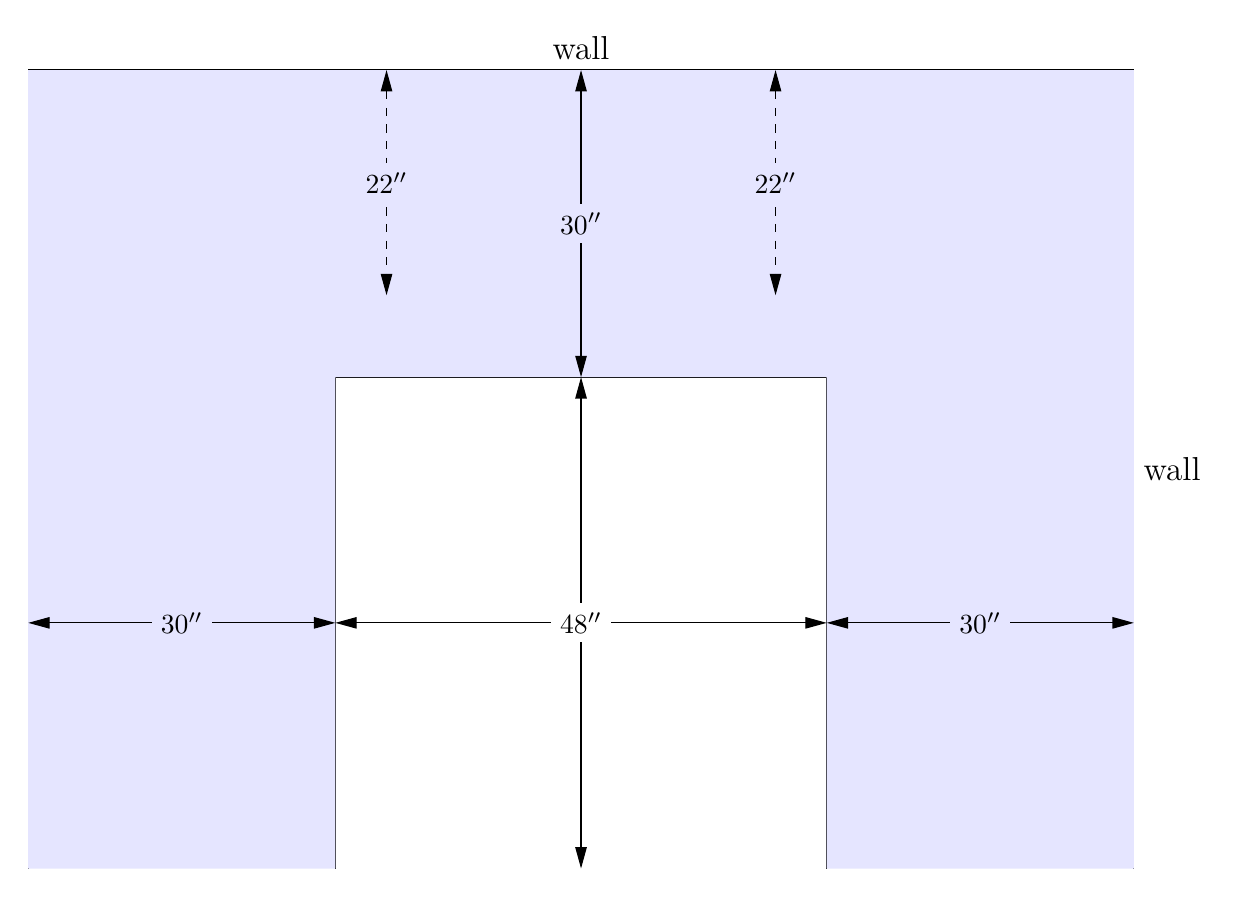
\begin{tikzpicture}[scale=0.13]
  % Define points.
  \coordinate   (p11) at (  0, 78);
    \coordinate (p14) at ( 35, 78);
    \coordinate (p15) at ( 54, 78);
    \coordinate (p16) at ( 73, 78);
    \coordinate (p19) at (108, 78);
  \coordinate   (p24) at ( 35, 67);
    \coordinate (p26) at ( 73, 67);
  \coordinate   (p35) at ( 54, 63);
  \coordinate   (p44) at ( 35, 56);
    \coordinate (p46) at ( 73, 56);
  \coordinate   (p53) at ( 30, 48);
    \coordinate (p55) at ( 54, 48);
    \coordinate (p57) at ( 78, 48);
  \coordinate   (p69) at (108, 39);
  \coordinate   (p71) at (  0, 24);
    \coordinate (p72) at ( 15, 24);
    \coordinate (p73) at ( 30, 24);
    \coordinate (p75) at ( 54, 24);
    \coordinate (p77) at ( 78, 24);
    \coordinate (p78) at ( 93, 24);
    \coordinate (p79) at (108, 24);
  \coordinate   (p81) at (  0,  0);
    \coordinate (p83) at ( 30,  0);
    \coordinate (p85) at ( 54,  0);
    \coordinate (p87) at ( 78,  0);
    \coordinate (p89) at (108,  0);
  % Put "wall" above drawing.
  \draw (p15) node[above] {\large wall};
  % Plot outer edge.
  \draw (p81) -- (p11) -- (p19) -- (p89);
  % Plot inner edge.
  \draw (p83) -- (p53) -- (p57) -- (p87);
  % Color the counter. 
  \fill[blue!10] (p81) -- (p11) -- (p19) -- (p89) -- (p87) -- (p57) -- (p53) -- (p83) -- cycle;
  % Vertical measurement lines.
  \draw[dashed, arrows = {Stealth[inset=0pt, angle=30:8pt]-Stealth[inset=0pt, angle=30:8pt]}]
    (p14) -- (p44);
  \draw (p24) node[fill=blue!10] {$22''$};
  \draw[arrows = {Stealth[inset=0pt, angle=30:8pt]-Stealth[inset=0pt, angle=30:8pt]}] (p15) -- (p55);
  \draw (p35) node[fill=blue!10] {$30''$};
  \draw[dashed, arrows = {Stealth[inset=0pt, angle=30:8pt]-Stealth[inset=0pt, angle=30:8pt]}]
    (p16) -- (p46);
  \draw (p26) node[fill=blue!10] {$22''$};
  \draw[arrows = {Stealth[inset=0pt, angle=30:8pt]-Stealth[inset=0pt, angle=30:8pt]}] (p55) -- (p85);
  % Horizontal measurement lines.
  \draw[arrows = {Stealth[inset=0pt, angle=30:8pt]-Stealth[inset=0pt, angle=30:8pt]}] (p71) -- (p73);
  \draw (p72) node[fill=blue!10] {$30''$};
  \draw[arrows = {Stealth[inset=0pt, angle=30:8pt]-Stealth[inset=0pt, angle=30:8pt]}] (p73) -- (p77);
  \draw (p75) node[fill=white] {$48''$};
  \draw[arrows = {Stealth[inset=0pt, angle=30:8pt]-Stealth[inset=0pt, angle=30:8pt]}] (p77) -- (p79);
  \draw (p78) node[fill=blue!10] {$30''$};
  % Put "wall" to the right of drawing.
  \draw (p69) node[right] {\large wall};
\end{tikzpicture}
\end{VerbatimOut}

\MyIO


\begin{VerbatimOut}{z.out}

\subsection{Fourier transform example}
\index{Fourier transform \TikZLogo\ example}
\todoindex{Fourier transform \TikZLogo\ example}
  
The Fourier transform decomposes a function
into the frequencies that make it up.
The inverse Fourier transformation combines the contributions
of all the different frequencies to recover the original function.

(Mark Senn {\tt\char'074}mark@purdue.edu{\tt\char'076} wrote sales@aavos.be on 2021-09-03
to ask permission
to use
\href{https://aavos.eu/glossary/fourier-transform/}{Fourier transform}
as the starting point
for an example \TikZLogo\ figure.  
Dominique Demurie {\tt\char'074}sales@aavos.be{\tt\char'076} replied
on 2021-09-06 with
``I think it is not an original drawing from us either.
We had it for years on our website,
but I cannot remember where we got it from.
We don't mind you using it for a thesis.'')

% Run this with
%     pdflatex --shell-escape t
% That makes the t.table.* files.
%
% See
%     https://ctan.math.washington.edu/tex-archive/graphics/pgf/base/doc/pgfmanual.pdf
%     PAGE    TOPIC
%      655    decorations.text library to draw text 
%     1221    animations
%
% for text decorations, which includes text along a path information.
% Also see
%     https://tex.stackexchange.com/questions/427454/tikz-3dplot-and-rotation-of-coordinates
%     https://tex.stackexchange.com/questions/67573/tikz-shift-and-rotate-in-3d
%     http://tug.ctan.org/graphics/pgf/contrib/tikz-3dplot/tikz-3dplot_documentation.pdf
%     https://tex.stackexchange.com/questions/45848/rotate-node-text-and-use-relative-positioning-in-tikz
  
% was scale = 2
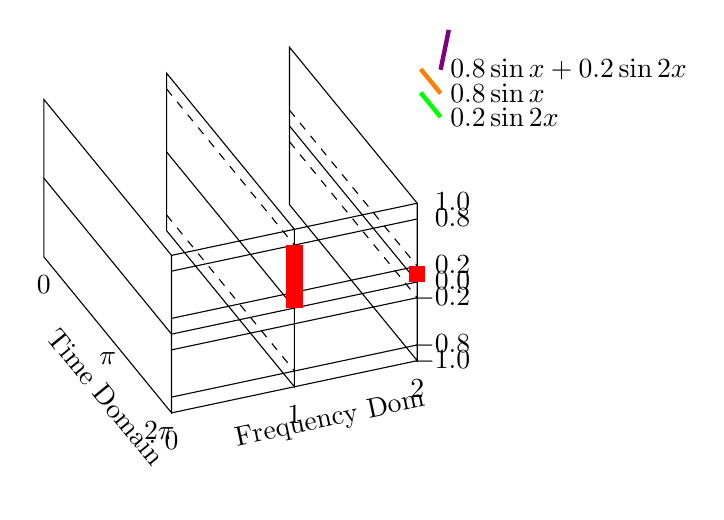
\begin{tikzpicture}[domain=0:6.283185, rotate around y=-55, scale=1]

  % total plot
  \begin{scope}[canvas is xy plane at z=0]
    \node[below=3pt] at (0,        -1) {0};
    \node[below=3pt] at (3.141593, -1) {$\pi$};
    \node[below=5pt] at (5.683185, -1) {$2\pi$};
    \draw[ultra thick,color=violet] plot[id=total,smooth] function{0.8*sin(x)+0.2*sin(8*x)};
    \draw[thin,color=black] (0,-1) -- (0,1) -- (6.283185,1) -- (6.283185,-1) -- cycle;
    \draw[thin,color=black] (0,0) -- (6.283185,0);
    \path[decorate,decoration={text along path,
% |\LARGE|
      text={Time Domain}}] (0.1,-2) -- (6.283185,-2); 
    % $s(t)$
  \end{scope}

  % tall plot
  \begin{scope}[canvas is xy plane at z=-1.5]
    \draw[dashed] (0,0.8) -- (6.283185,0.8);
    \draw[dashed] (0,-0.8) -- (6.283185,-0.8);
    \draw[thick,color=orange] plot[id=tall,smooth] function{0.8*sin(x)};
    \draw[thin,color=black] (0,-1) -- (0,1) -- (6.283185,1) -- (6.283185,-1) -- cycle;
    \draw[thin,color=black] (0,0) -- (6.283185,0);
  \end{scope}

  % short plot
  \begin{scope}[canvas is xy plane at z=-3.0]
    \draw[dashed] (0, 0.2) -- (6.283185,  0.2);
    \draw[dashed] (0,-0.2) -- (6.283185, -0.2);
    \draw[thick,color=green] plot[id=short,smooth] function{0.2*sin(2*x)};
    \draw[thin,color=black] (0,-1) -- (0,1) -- (6.283185,1) -- (6.283185,-1) -- cycle;
    \draw[thin,color=black] (0,0) -- (6.283185,0);
  \end{scope}

  % frequency plot
  \begin{scope}[canvas is zy plane at x=6.283185]
    \node[below=3pt] at ( 0.0,-1) {0};
    \node[below=3pt] at (-1.5,-1) {1};
    \node[below=3pt] at (-3.0,-1) {2};
    \draw[thin,color=black] (0,-1.0) -- (-3.0,-1.0);  \node[above=-9pt] at (-3.3,-1.0) {$-1.0$};
    \draw[thin,color=black] (0,-0.8) -- (-3.0,-0.8);  \node[above=-9pt] at (-3.3,-0.8) {$-0.8$};
    \draw[thin,color=black] (0,-0.2) -- (-3.0,-0.2);  \node[above=-9pt] at (-3.3,-0.2) {$-0.2$};
    \draw[thin,color=black] (0, 0.0) -- (-3.0, 0.0);  \node[above=-9pt] at (-3.3, 0.0) {$\phantom{-}0.0$};
    \draw[thin,color=black] (0, 0.2) -- (-3.0, 0.2);  \node[above=-9pt] at (-3.3, 0.2) {$\phantom{-}0.2$};
    \draw[thin,color=black] (0, 0.8) -- (-3.0, 0.8);  \node[above=-9pt] at (-3.3, 0.8) {$\phantom{-}0.8$};
    \draw[thin,color=black] (0, 1.0) -- (-3.0, 1.0);  \node[above=-9pt] at (-3.3, 1.0) {$\phantom{-}1.0$};
    \draw[line width=6pt,color=red] (-1.5,0) -- (-1.5,0.8);
    \draw[line width=6pt,color=red] (-3.0,0) -- (-3.0,0.2);
    \path[decorate,decoration={text along path,
% |\LARGE|
      text={Frequency Domain}}] (-0.8,-1.6) -- (-3.0,-1.6); 
    % $S(\omega)$
  \end{scope}

  %% legend
  %% Wolfram Language code:
  %%     In[1]:= ry[theta_] :=
  %%     {
  %%         {Cos[theta Degree],  0, Sin[theta Degree]},
  %%         {0,                  1, 0},
  %%         {-Sin[theta Degree], 0, Cos[theta Degree]}
  %%     }
  %%
  %%     ry[55] . {Pi, 0.7, -3.5}
  %%     # Out[] = {-1.06509, 0.7, -4.58096}
  %%     ry[55] . {(3/4)Pi, 0.7, -3.5}
  %%     # Out[] = {-1.51557, 0.7, -3.9376}

  \draw[ultra thick,color=violet] (2.45782, 1.7, -4.33538) -- (1.06509, 0.7, -4.58096);
    \node[right] at                                            (1.06509, 0.7, -4.58096) {$0.8\sin x + 0.2\sin 2x$};
  \draw[ultra thick,color=orange] ( 0.08509, 0.4, -4.58096) -- (1.06509, 0.4, -4.58096);
    \node[right] at                                            (1.06509, 0.4, -4.58096) {$0.8\sin x$};
  \draw[ultra thick,color=green]  ( 0.08509, 0.1, -4.58096) -- (1.06509, 0.1, -4.58096);
    \node[right] at                                            (1.06509, 0.1, -4.58096) {$0.2\sin 2x$};
\end{tikzpicture}
\end{VerbatimOut}

\MyIO


\begin{VerbatimOut}{z.out}

\subsection{Glider example}
\ix{Hirzel, Alex}
\index{glider \TikZLogo\ example}
\todoindex{glider \TikZLogo\ example}

The glider
is a pattern from the Game of Life,
and it's used as an emblem representing the hacker community.

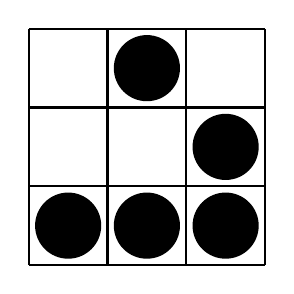
\begin{tikzpicture}[thick]
  \draw (0,0) grid (3,3);
  \foreach \c in {(0,0), (1,0), (2,0), (2,1), (1,2)}
    \fill \c + (0.5,0.5) circle (0.42);
\end{tikzpicture}
\end{VerbatimOut}

\MyIO


\begin{VerbatimOut}{z.out}

\newpage

\subsection{Tree example}
\ix{???, ???}
\index{tree \TikZLogo\ example}
\todoindex{tree \TikZLogo\ example}

{
  \def\f#1#2{$\displaystyle\frac #1#2$}
  \begin{tikzpicture}%
  [%
    level 1/.style={sibling distance=60mm},
    level 2/.style={sibling distance=30mm},
    level 3/.style={sibling distance=15mm}
  ]
    \node {\f 11}
      child {node {$\displaystyle\frac 12$}
        child {node {\f 13}
          child {node {\f 14}}
          child {node {\f 48}}
        }
        child {node {\f 32}
          child {node {\f 35}}
          child {node {\f 52}}
        }
      }
      child {node {\f 21}
        child {node {\f 23}
          child {node {\f 25}}
          child {node {\f 53}}
        }
        child {node {\f 31}
          child {node {\f 34}}
          child {node {\f 41}}
        }
      };
  \end{tikzpicture}    

\vspace*{4pt}
The node with value \f nd\\[2pt]
\indent\hspace*{4\parindent}
\begin{tabular}{@{}llll@{}}
  \bfseries with additional conditions& \bfseries has& \bfseries with value\\
  \noalign{\vspace{2pt}}
  (none)&                     left child&     \f n{{n+d}}\\
  \noalign{\vspace{12pt}}
  (none)&                     right child&    \f {{n+d}}d\\
  \noalign{\vspace{12pt}}
  $n<d$&                      parent&         \f n{{d-n}}\\
  \noalign{\vspace{12pt}}
  $n=d$&                      no parent&      (not applicable)\\
  \noalign{\vspace{12pt}}
  $n>d$&                      parent&         \f {{n-d}}d\\
\end{tabular}
}
\end{VerbatimOut}

\MyIO

\begin{VerbatimOut}{z.out}


\subsection{Yin and yang example}

This Yin and yang example was done by Thomas G. Kristensen \cite{kristensen}.
This is the ``traditional Taijitu symbol from Chinese philosophy''.
\ix{Kristensen, Thomas G.//Taijitu symbol//Yin and yang symbol}

\index{TikZ@\TikZLogo}  
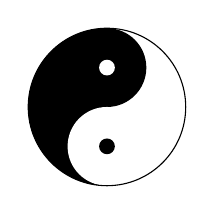
\begin{tikzpicture}
  % Yin and yang
  % Author: Thomas G. Kristensen
  
  % color one half of a unit circle                                              
  \begin{scope}
    \clip (0,0) circle (1cm);
    \fill[black] (0cm,1cm) rectangle (-1cm, -1cm);
  \end{scope}

  % fill heads                                                                   
  \fill[black] (0,0.5) circle (0.5cm);
  \fill[white] (0,-0.5) circle (0.5cm);

  % fill eyes                                                                    
  \fill[white] (0,0.5) circle (0.1cm);
  \fill[black] (0,-0.5) circle (0.1cm);

  % outer line                                                                   
  \draw (0,0) circle (1cm);

\end{tikzpicture}
\end{VerbatimOut}

\MyIO


\begin{VerbatimOut}{z.out}

\section{Wolfram Language (Mathematica uses this)}
\ix{Mathematica}
\ix{Wolfram Language}

\lightgreen{Wolfram Language can be set up to use \LaTeX\ fonts.}

\includegraphics{gr-mathematica.pdf}

This is the |misc/gr-mathematica.ma| input file
\MyI{misc/gr-mathematica.ma}

I typed, on Linux,
\Shell{math < gr-mathematica.ma}
in the |misc| subdirectory
to make the |graphics/gr-mathematica.pdf| output file.
\end{VerbatimOut}

\MyIO


  % Ignore these references.
  %\ProvidesFile{ap-ignore-these-references.tex}[2022-10-05 ignore these references appendix]

\begin{VerbatimOut}{z.out}
\chapter{IGNORE THESE REFERENCES---THEY ARE WRONG}
\end{VerbatimOut}

\MyIO


\begin{VerbatimOut}{z.out}

You may have seen these references on the web.
Ignore them---they're wrong.

\noindent
\textbf{Purdue Online Writing Lab, IEEE Reference List}
\cite{owl}

The IEEE
(The world's largest technical professional organization
for the advancement
of technology)
has changed their references format from,
for example,

\noindent
\begin{tabular}{@{}ll@{}}
\noalign{\vspace*{6pt}}
  [1]& W. K. Chen, Linear Networks and Systems. Belmont, CA: Wadsworth Press,\\
  \multispan{2}{2003.\hfil}\\
\noalign{\vspace*{6pt}}
\noalign{\noindent to}
\noalign{\vspace*{6pt}}
  [1]& W. K. Chen, Linear Networks and Systems. Belmont, CA: Wadsworth Press,\\
  & 2003.\hfil\\
\noalign{\vspace*{6pt}}
\end{tabular}
See
\cite[page~2]{ieeedataport}.
\end{VerbatimOut}

\MyIO


% BL  @online{owl,
% BT  @misc{owl,
%     author  = {Purdue Online Writing Lab},
%     title   = {IEEE Reference List},
%     url     = {https://owl.purdue.edu/owl/research_and_citation/ieee_style/reference_list.html},
% BL  urldate = {2022-03-17},
% }
% 
% BL  @online{ieeedataport,
% BT  @misc{ieeedataport,
%     author  = {IEEEDataPort},
%     title   = {How too Cite References: IEEE Documentation Style},
%     url     = {https://ieee-dataport.org/sites/default/files/analysis/27/IEEE%20Citation%20Guidelines.pdf},
% BL  urldate = {2022-03-17},
% }  


  % Logos.
  %\ProvidesFile{ap-logos.tex}[2022-10-05 logos appendix]

\begin{VerbatimOut}{z.out}
\chapter{LOGOS}

These logos are defined in |pa-logos.sty|:

\begin{tabular}{@{}ll@{}}
  \toprule
  \bfseries Input& \bfseries Output\\
  \midrule
  % From thesis.tex
  %     \newcommand{\tabularspace}{\noalign{\vspace*{2pt}}}
  % \tabularspace
  \verb+\AMSmathLogo+& \AMSmathLogo\\[2pt]
  \verb+\BibLaTeXLogo+& \BibLaTeXLogo\\[2pt]
  \verb+\BiberLogo+& \BiberLogo\\[2pt]
  \verb+\CalligraphicAMSLaTeXLogo+& \CalligraphicAMSLaTeXLogo\\[2pt]
  \verb+\CircuiTikZLogo+& \CircuiTikZLogo\\[2pt]
  \verb+\CTANLogo{\texttt{CTAN}\xspace}+& \CTANLogo\\[2pt]
  \verb+\LaTeXLogo+& \LaTeXLogo\\[2pt]
  \verb+\LuaLaTeXLogo+& \LuaLaTeXLogo\\[2pt]
  \verb+\METAFONTLogo+& \METAFONTLogo\\[2pt]
  \verb+\METAPOSTLogo+& \METAPOSTLogo\\[2pt]
  \verb+\MetaPostLogo+& \MetaPostLogo\\[2pt]
  \verb+\NonCalligraphicAMSLaTeXLogo+& \NonCalligraphicAMSLaTeXLogo\\[2pt]
  \verb+\PurdueThesisLogo+& \PurdueThesisLogo\\[2pt]
  \verb+\PuThLogo+& \PuThLogo\\[2pt]
  \verb+\TeXLogo+& \TeXLogo\\[2pt]
  \verb+\TeXLiveLogo+& \TeXLiveLogo\\[2pt]
  \verb+\TikZLogo+& \TikZLogo\\[2pt]
  \verb+\TEXUsersGroupLogo+& \TeXUsersGroupLogo\\[2pt]
  \verb+\TUGboatLogo+& \TUGboatLogo\\[2pt]
  \bottomrule
\end{tabular}
\end{VerbatimOut}

\MyIO


  % Miscellaneous.
  %\ProvidesFile{ap-miscellaneous.tex}[2022-10-05 miscellaneous appendix]

\begin{VerbatimOut}{z.out}
\chapter{MISCELLANEOUS}
\ix{miscellaneous//Miscellaneous appendix}
\end{VerbatimOut}

\MyIO


\begin{VerbatimOut}{z.out}
Demonstrate using a long Hungarian umlaut
(double acute)
(\H{o})
in text and bibligraphy
\cite{erdos1992}.
\end{VerbatimOut}

\MyIO

  
  % Numbers and Units.
  %\ProvidesFile{ap-numbers-and-units.tex}[2022-10-05 numbers and units appendix]

%  Primary sources:
%      See https://www.bipm.org/utils/common/pdf/si-brochure/SI-Brochure-9-EN.pdf.
%      See https://www.nist.gov/pml/special-publication-811/nist-guide-si-chapter-4-two-classes-si-units-and-si-prefixes.
%
%  Notes:
%      See https://www.iso.org/standard/60241.html.

% Historic Vote Ties Kilogram and Other Units to Natural Constants
% NIST
% https://www.nist.gov/news-events/news/2018/11/historic-vote-ties-kilogram-and-other-units-natural-constants
% created 2018-11-16
% updated 2018-12-21
% last retrieved 2018-12-22

% https://www.bipm.org/utils/common/pdf/CGPM-2018/26th-CGPM-Resolutions.pdf
% Resolutions adopted
% 26^e CGPM
% Versailes
% 13--16 November 2018
% last retrieved 2018-12-30

% author Joseph Wright
% date 2018-05-17
% retrieved 2018-12-29
% url ftp://ftp.dante.de/tex-archive/macros/latex/exptl/siunitx/siunitx.pdf


\begin{VerbatimOut}{z.out}
\chapter{NUMBERS AND UNITS}
\end{VerbatimOut}

\MyIO


\begin{VerbatimOut}{z.out}

Note to self: scientific prefixes, scientific suffixes, tables.

The puthesis 2.0 and after documentclass uses the siunitx
package with some extra definitions in the puthesis.cls
file to do numbers and units.
\end{VerbatimOut}

\MyIO


\begin{VerbatimOut}{z.out}

\section{Number Examples}
\end{VerbatimOut}

\MyIO


\begin{VerbatimOut}{z.out}
\noindent\begin{tabular}{@{}lll@{}}
  \bfseries Input& \bfseries Output& \bfseries Comment\\
  \tabularspace
  \verb+\num{-0.12345}+& \num{-0.12345}& note the small space after the ``3''\\
  \verb+\num{-0.1234}+&
    \num{-0.1234}&
    note no space between the ``3'' and ``4''\\
  \verb+\num{-.123}+& \num{-.123}& the ``0.'' is inserted automatically\\
  \verb+\num{123}+& \num{123}\\
  \verb+\num{1234}+& \num{1234}\\
  \verb+\num{12345}+& \num{12345}& note the small space after the ``2''\\
  \verb+\num{2e4}+& \num{2e4}\\
  \verb+\num{e5}+& \num{e5}\\
  \verb+\num{2.34567e6}+&
    \num{2.34567e6}&
    note the small space after the ``5''\\
\end{tabular}
\end{VerbatimOut}

\MyIO


\begin{VerbatimOut}{z.out}

\section{Unit Examples}
\end{VerbatimOut}

\MyIO


\begin{VerbatimOut}{z.out}

See page~\pageref{se:Complete-List-of-Units}
for the complete list
of units defined by \PurdueThesisLogo.

\noindent\begin{tabular}{@{}lll@{}}
  \bfseries Input& \bfseries Output& \bfseries Comment\\
  \tabularspace
  \verb+\si{\kg}+& \si{\kg}& kilogram\\
  \verb+\si{\m}+& \si{\m}& meter\\
  \verb+\si{\kg\per\m\squared}+&
    \si{\kg\per\m\squared}&
    \(= \si{\kg}/\si{\m\squared}\)\\
\end{tabular}
\end{VerbatimOut}

\MyIO


\begin{VerbatimOut}{z.out}

\section{Combined Number and Unit Examples}
\end{VerbatimOut}

\MyIO


\begin{VerbatimOut}{z.out}
\begin{tabular}{@{}lll@{}}
  \bfseries Input& \bfseries Output& \bfseries Comment\\
  \tabularspace
  \verb+\SI{12}{\kg}+& \SI{12}{\kg}& 12 kilograms\\
  \verb+\SI{34}{\m}+&  \SI{34}{\m}& 34 meters\\
  % The next input line is too wide for the margins
  % so I'm splitting it into pieces.
  \verb+\SI{4.5e3}{\kg\per\m\squared}+&
    \SI{4.5e3}{\kg\per\m\squared}&
    \(= \num{4.5e3}\,\si{\kg}/\si{\m\squared}\)\\
\end{tabular}
\end{VerbatimOut}

\MyIO


\begin{VerbatimOut}{z.out}

How many seconds are in a non-leap year that does not have any leap seconds?
% I tried several things and couold not get \cancel to work with \per.
% Mark Senn    2019-12-29
\begin{align*}
           \frac{\SI{365}{\cancel\d}}{\si{\y}}
    \times \frac{\SI{24}{\cancel\h}}{\si{\cancel\d}}
    \times \frac{\SI{60}{\cancel\min}}{\si{\cancel\h}}         
    \times \frac{\SI{60}{\s}}{\si{\cancel\min}}         
    % From http://www.emerson.emory.edu/services/latex/latex_119.html
    %     Spacing in Math Mode
    %     In a math environment, LaTeX ignores the spaces you type
    %     and puts in the spacing that it thinks is best. LaTeX formats
    %     mathematics the way it's done in mathematics texts. If you
    %     want different spacing, LaTeX provides the following four
    %     commands for use in math mode:
    %         \; - a thick space
    %         \: - a medium space
    %         \, - a thin space
    %         \! - a negative thin space
    & = \num{31536000}\;\frac{\si{\s}}{\si{\y}}\\
    & = \SI{31536000}{\s\per\y}\\
    & \approx \SI{3e7}{\s\per\y}\\
    & \approx \text{30 million\,}\si{\s\per\y}\\
\end{align*}
\end{VerbatimOut}

\MyIO


\begin{VerbatimOut}{z.out}

\section{Binary Prefixes}
\end{VerbatimOut}

\MyIO


\begin{VerbatimOut}{z.out}

The \verb+\kibi+ \ldots \verb+\yobi+
commands are defined immediately after the \verb+\usepackage{siunitx}+ command
in the PurdueThesis.cls file.
\end{VerbatimOut}

\MyIO


\begin{VerbatimOut}{z.out}

\newcolumntype{m}{>{$}r<{$}}  % math mode version of "r" column type
\renewcommand{\t}[4]{\(2^{#1}\) bytes is a #2, \(10^{#3}\) bytes is a #4}
\begin{tabular}{@{}mllll@{}}
  \multicolumn{1}{l}{\bfseries Power}&
    \bfseries Prefix&
    \bfseries Symbol&
    \bfseries Command&
    \bfseries Comment\\
  \tabularspace
  10& kibi& \unit{\kibi\nounit}& \verb+\si{\kibi}+& \t{10}{KB}{3}{KiB}\\
  20& mebi& \unit{\mebi\nounit}& \verb+\si{\mebi}+& \t{20}{MB}{6}{MiB}\\
  30& gibi& \unit{\gibi\nounit}& \verb+\si{\gibi}+& \t{30}{GB}{9}{GiB}\\
  40& tebi& \unit{\tebi\nounit}& \verb+\si{\tebi}+& \t{40}{TB}{12}{TiB}\\
  50& pebi& \unit{\pebi\nounit}& \verb+\si{\pebi}+& \t{50}{PB}{15}{PiB}\\
  60& exbi& \unit{\exbi\nounit}& \verb+\si{\exbi}+& \t{60}{EB}{18}{EiB}\\
  70& zebi& \unit{\zebi\nounit}& \verb+\si{\zebi}+& \t{70}{ZB}{21}{ZiB}\\
  80& yobi& \unit{\yobi\nounit}& \verb+\si{\yobi}+& \t{80}{YB}{24}{YiB}\\
\end{tabular}
\end{VerbatimOut}

\MyIO


\begin{VerbatimOut}{z.out}

\section{Decimal Prefixes}
\end{VerbatimOut}

\MyIO

\begin{VerbatimOut}{z.out}

\newcolumntype{m}{>{$}r<{$}}  % math mode version of "r" column type
\begin{tabular}{@{}mllll@{}}
  \multicolumn{1}{l}{\bfseries Power}&
    \bfseries Prefix&
    \bfseries Symbol&
    \bfseries Command&
    \bfseries Comment\\
  \tabularspace
  -24& yocto& \unit{\yocto\nounit}& \verb+\si{\yocto}+\\
  -21& zepto& \unit{\zepto\nounit}& \verb+\si{\zepto}+\\
  -18& atto&  \unit{\atto\nounit}&  \verb+\si{\atto}+\\
  -15& femto& \unit{\femto\nounit}& \verb+\si{\femto}+\\
  -12& pico&  \unit{\pico\nounit}&  \verb+\si{\pico}+\\
   -9& nano&  \unit{\nano\nounit}&  \verb+\si{\nano}+\\
   -6& micro& \unit{\micro\nounit}& \verb+\si{\micro}+\\
   -3& milli& \unit{\milli\nounit}& \verb+\si{\milla}+\\
   -2& centi& \unit{\centi\nounit}& \verb+\si{\centi}+\\
   -1& deci&  \unit{\deci\nounit}&  \verb+\si{\deci}+\\
    1& deca&  \unit{\deca\nounit}&  \verb+\si{\deca}+\\
    1& deka&  \unit{\deka\nounit}&  \verb+\si{\deka}+& same as \verb+\si{\deca}+\\
    2& hecto& \unit{\hecto\nounit}& \verb+\si{\hecto}+\\
    3& kilo&  \unit{\kilo\nounit}&  \verb+\si{\kilo}+\\
    6& mega&  \unit{\mega\nounit}&  \verb+\si{\mega}+\\
    9& giga&  \unit{\giga\nounit}&  \verb+\si{\giga}+\\
   12& tera&  \unit{\tera\nounit}&  \verb+\si{\tera}+\\
   15& peta&  \unit{\peta\nounit}&  \verb+\si{\peta}+\\
   18& exa&   \unit{\exa\nounit}&   \verb+\si{\exa}+\\
   21& zetta& \unit{\zetta\nounit}& \verb+\si{\zetta}+\\
   24& yotta& \unit{\yotta\nounit}& \verb+\si{\yotta}+\\
\end{tabular}
\end{VerbatimOut}

\MyIO


\begin{VerbatimOut}{z.out}

\section{SI Units}
\end{VerbatimOut}

\MyIO


\begin{VerbatimOut}{z.out}

The International System of Units
(SI)
% !!! Doing
% !!!     \include{tipa}
% !!! in thesis.tex so \textprimstress works
% !!! apparently causes problems with math commands.
% !!! Figure out why the following doesn't work later.
% (%
%   SI,
%   abbreviated from the French Syst\`eme International
%   (d\textprimstress unit\'es)%
% )
is the modern form of the metric system.
There are seven SI base units:

\hspace{40pt}
\begin{tabular}{@{}lll@{}}
  \tabularspace
  \bfseries Name& \bfseries Unit Of&         \bfseries Symbol\\
  \tabularspace
  ampere&         electrical current&        \si{\ampere}\\
  candela&        luminous intensity&        \si{\candela}\\
  kelvin&         thermodynamic temperature& \si{\kelvin}\\
  kg&             mass&                      \si{\kilogram}\\
  meter&          length&                    \si{\meter}\\
  mole&           amount of substance&       \si{\mole}\\
  second&         time&                      \si{\second}\\
\end{tabular}
\end{VerbatimOut}

\MyIO


\begin{VerbatimOut}{z.out}

\section{Complete List of Units}
\label{se:Complete-List-of-Units}
\end{VerbatimOut}

\MyIO

\begin{VerbatimOut}{z.out}

{%
  \ZZbaselinestretch{1}
  \newcommand\vsp{\noalign{\vspace*{6pt}}}
  % From
  % https://tex.stackexchange.com/questions/31508/flushleft-with-p-option-in-tabular
  %     It's necessary to use the \arraybackslash in the last column,
  %     otherwise \\ would not end the table row.  You can use \newline
  %     to end lines in the last column cells (and the regular \\ in
  %     the other column cells).
  %     ...
  %     If you need it often, consider defining a new column type using
  %     array features, as I did here:
  %         \newcolumntype{P}[1]{>{\raggedright\arraybackslash}p{#1}}
  \newcolumntype{P}[1]{>{\raggedright\arraybackslash}p{#1}}%
% \begin{longtable}{@{}P{1.4in}P{1in}llP{1.8in}@{}}
% \begin{longtable}{@{}P{1in}P{1in}llP{1.8in}@{}}
% \begin{longtable}{@{}P{1.2in}P{1in}llP{1.8in}@{}}
% \begin{longtable}{@{}P{90.72pt}P{1in}llP{1.8in}@{}}  % 1.2in (86.72pt) + 4pt = 90.72pt
  \begin{longtable}{@{}P{1.4in}P{1in}llP{1.8in}@{}}% 1.2in (86.72pt) + 4pt = 90.72pt
      \caption{Units and Corresponding Symbols}\\
      \bfseries Name&
        \bfseries Unit Of&
        \bfseries Symbol&
        \bfseries Command&
        \bfseries Is equal to\\
      \vsp
    \endfirsthead
      \caption[]{~\emph{continued}}\\
      \bfseries Name&
        \bfseries Unit Of&
        \bfseries Symbol&
        \bfseries Command&
        \bfseries Is equal to\\
      \vsp
    \endhead
      \vsp
      % I don't know why the \hspace*{-7.5mm} was
      % needed to center this horizontally.
      \multicolumn{5}{@{}c@{}}{\hspace*{-7.5mm}\emph{continued on next page}}%
    \endfoot    
    \endlastfoot
    ampere&
      electrical current&
      \si{\A}&
      \verb+\si{\A}+&
      (SI base unit)\\
    \quad picoampere&
      \ditto&
      \si{\pA}&
      \verb+\si{\pA}+&
      \SI{e-12}{\A}\\ 
    \quad nanoampere&
      \ditto&
      \si{\nA}&
      \verb+\si{\nA}+&
      \SI{e-9}{\A}\\
    \quad microampere&
      \ditto&
      \si{\uA}&
      \verb+\si{\uA}+&
      \SI{e-6}{\A}\\
    \quad milliampere&
      \ditto&
      \si{\mA}&
      \verb+\si{\mA}+&
      \SI{e-3}{\A}\\
    \quad kiloampere&
      \ditto&
      \si{\kA}&
      \verb+\si{\kA}+&
      \SI{e3}{\A}\\
    \vsp
    % \aa ngstr\"om&
    %   length&
    %   \si{\AA}&
    %   \verb+\si{\AA}+&
    %   \SI{e-10}{\m}\\
    \vsp
    arcminute&
      plane angle&
      \si{\arcmin}&
      \verb+\si{\arcmin}+&
      % Changed
      %     \SI{1/60}{\degree}\\
      % to
      1/60\unit{\degree\nounit}\\
    arcsecond&
      plane angle&
      \si{\arcsec}&
      \verb+\si{\arcsec}+&
      % Changed
      %     \SI{1/60}{\arcmin}\\
      % to
      1/60\unit{\arcmin\nounit}\\
    \vsp
    astronomical unit&
      length&
      \si{\au}&
      \verb+\si{\au}+&
      mean earth to\newline sun distance\\
    \vsp
    % From
    %     siunitx - A comprehensive (SI) units package
    %     Joseph Wright
    %     Released 2021-08-04
    %     (this describes v3.0.24, last revised 2021-08-04)
    %     https://mirror.las.iastate.edu/tex-archive/macros/latex/contrib/siunitx/siunitx.pdf
    % page 51:
    %     ...the unit \atomicmassunit has similar deprecated status:
    %     this was listed as with experimentally-determined units
    %     in the 8th Edition of the si Brochure but is equivalent
    %     to the dalton, a unit which remains accepted.
    % atomic mass unit&
    %   mass&
    %   \si{\amu}&
    %   \verb+\si{\amu}+&
    %   \(1/12\) mass of\newline carbon-12 atom\\
    % \vsp
    bar&
      pressure&
      \si{\bar}&
      \verb+\si{\bar}+&
      \SI{e-5}{\Pa}\\
    \quad millibar&
      \ditto&
      \si{\mbar}&
      \verb+\si{\mbar}+&
      \SI{e-3}{\bar}\\
    \vsp
    barn&
      area&
      \si{\b}&
      \verb+\si{\b}+&
      \SI{e-28}{\m\squared}\\
    \vsp
    becquerel&
      radioactivity&
      \si{\Bq}&
      \verb+\si{\Bq}+&
      one radioactive\newline decay per second\\
    \vsp
    bel&
      sound intensity&
      \si{\B}&
      \verb+\si{\B}+&
      10 decibels\\
    \quad decibel&
      \ditto&
      \si{\dB}&
      \verb+\si{\dB}+&
      \SI{e-1}{\B}\\
    \vsp
    bohr&
      length&
      \si{\bohr}&
      \verb+\si{\bohr}+&
      distance between\newline nucleus and electron\newline in hydrogen atom\\
    \vsp
    bushel&
      quantity&
      \si{\bu}&
      \verb+\si{\bu}+&
      see \cite{wikipedia-bushel}\\
    \vsp
    candela&
      luminous intensity&
      \si{\cd}&
      \verb+\si{\cd}+&
      (SI base unit)\\
    \vsp
    coulomb&
      electrical charge&
      \si{\C}&
      \verb+\si{\C}+&
      \si{\A\per\s}\\
    \vsp
    dalton&
      mass&
      \si{\Da}&
      \verb+\si{\Da}+&
      another name for\newline atomic mass unit\\
    \vsp
    day&
      time&
      \si{\d}&
      \verb+\si{\d}+&
      \SI{86400}{\s}\\
    \vsp
    degree&
      plane angle&
      \si{\degree}&
      \verb+\si{\degree}+&
      1/360 of a cicle\\
    \vsp
    degree Celsius&
      temperature&
      \si{\celsius}&
      \verb+\si{\celsius}+&
      xxx\\
    \vsp
    electron mass&
      mass&
      \si{\em}&
      \verb+\si{\em}+&
      xxx\\
    \vsp
    electronvolt&
      energy&
      \si{\eV}&
      \verb+\si{\eV}+&
      xxx\\
    \quad millielectronvolt&
      \ditto&
      \si{\meV}&
      \verb+\si{meV}+&
      \SI{e-3}{\eV}\\
    \quad kiloelectronvolt&
      \ditto&
      \si{\keV}&
      \verb+\si{keV}+&
      \SI{e3}{\eV}\\
    \quad megaelectronvolt&
      \ditto&
      \si{\MeV}&
      \verb+\si{MeV}+&
      \SI{e6}{\eV}\\
    \quad gigaelectronvolt&
      \ditto&
      \si{\GeV}&
      \verb+\si{\GeV}+&
      \SI{e9}{\eV}\\
    \quad teraelectronvolt&
      \ditto&
      \si{\TeV}&
      \verb+\si{\TeV}+&
      \SI{e12}{\eV}\\
    \vsp
    elementary charge&
      electrical charge&
      \si{\ec}&
      \verb+\si{\ec}+&
      \href{https://en.wikipedia.org/wiki/Elementary_charge}{\SI{\approx 1.6e19}{\C}}\\
    \vsp
    farad&
      electrical capacitance&
      \si{\F}&
      \verb+\si{\F}+&
      \si{\s\tothe{4}\A\squared\per\m\squared\per\kg}\\
    \quad femtofarad&
      \ditto&
      \si{\fF}&
      \verb+\si{\fF}+&
      \SI{e-15}{\F}\\
    \quad picofarad&
      \ditto&
      \si{\pF}&
      \verb+\si{\pF}+&
      \SI{e-12}{\F}\\
    \vsp
    foot&
      length&
      \si{\ft}&
      \verb+\si{\ft}+&
      \SI{0.3048}{\m}\\  % not an SI unit
    \vsp
    % gauss: The gauss, symbol G, sometimes Gs, is the cgs unit of measurement of magnetic flux.
    gray&
      absorbed dose of ionizing radiation&
      \si{\Gy}&
      \verb+\si{\Gy}+&
      \si{\J\per\kg}\\
    \vsp
    hartree&
      energy used in molecular orbital calculations&
      \si{\hartree}&
      \verb+\si{\hartree}+&
      xxx\\
    \vsp
    hectare&
      area&
      \si{\ha}&
      \verb+\si{\ha}+&
      \SI{e4}{\m\squared}\\
    \vsp
    henry&
      electrical inductance&
      \si{\H}&
      \verb+\si{\H}+&
      \si{\kg\m\squared\per\s\squared\per\A\squared}\\
    \vsp
    hertz&
      frequency&
      \si{\Hz}&
      \verb+\si{\Hz}+&
      \si{\per\s}\\
    \quad millihertz&
      \ditto&
      \si{\mHz}&
      \verb+\si{\mHz}+&
      \SI{e-3}{\Hz}\\
    \quad kilohertz&
      \ditto&
      \si{\kHz}&
      \verb+\si{\kHz}+&
      \SI{e3}{\Hz}\\
    \quad megahertz&
      \ditto&
      \si{\MHz}&
      \verb+\si{\MHz}+&
      \SI{e6}{\Hz}\\
    \quad gigahertz&
      \ditto&
      \si{\GHz}&
      \verb+\si{\GHz}+&
      \SI{e9}{\Hz}\\
    \quad terahertz&
      \ditto&
      \si{\THz}&
      \verb+\si{\THz}+&
      \SI{e12}{\Hz}\\
    \vsp
    horsepower&
      power&
      \si{\hp}&
      \verb+\si{\hp}+&
      \SI{\approx 745.7}{\W}, {\bfseries IMPORTANT:\newline
        see \href{https://en.wikipedia.org/wiki/Horsepower#Mechanical_horsepower}{Horsepower}}\\
        % not an SI unit
    \vsp
    hour&
      time&
      \si{\h}&
      \verb+\si{\h}+&
      \SI{3600}{\s}\\
    \vsp
    inch&
      length&
      \si{\in}&
      \verb+\si{\in}+&
      \SI{25.4}{\mm}\\  % not an SI unit
    \vsp
    joule&
      work or energy&
      \si{\J}&
      \verb+\si{\J}+&
      \si{\kg\m\squared\per\s\squared}\\
    \quad microjoule&
      \ditto&
      \si{\uJ}&
      \verb+\si{\uJ}+&
      \SI{e-6}{\J}\\
    \quad millijoule&
      \ditto&
      \si{\mJ}&
      \verb+\si{\mJ}+&
      \SI{e-3}{\J}\\
    \quad kilojoule&
      \ditto&
      \si{\kJ}&
      \verb+\si{\kJ}+&
      \SI{e3}{\J}\\
    \quad megajoule&
      \ditto&
      \si{\MJ}&
      \verb+\si{\MJ}+&
      \SI{e6}{\J}\\
    \vsp
    katal&
      catalytic activity&
      \si{\kat}&
      \verb+\si{\kat}+&
      \si{\mol\per\s}\\
    \vsp
    kelvin&
      thermodynamic temperature&
      \si{\K}&
      \verb+\si{\K}+&
      (SI base unit)\\
    \vsp
    kilogram&
      mass&
      \si{\kg}&
      \verb+\si{\kg}+&
      (SI base unit)\\
    \quad femtogram&
      \ditto&
      \si{\fg}&
      \verb+\si{\fg}+&
      \SI{e-15}{\g}\\
    \quad picogram&
      \ditto&
      \si{\pg}&
      \verb+\si{\pg}+&
      \SI{e-12}{\g}\\
    \quad nanogram&
      \ditto&
      \si{\ng}&
      \verb+\si{\ng}+&
      \SI{e-9}{\g}\\
    \quad microgram&
      \ditto&
      \si{\ug}&
      \verb+\si{\ug}+&
      \SI{e-6}{\g}\\
    \quad milligram&
      \ditto&
      \si{\mg}&
      \verb+\si{\mg}+&
      \SI{e-3}{\g}\\
    \quad gram&
      \ditto&
      \si{\g}&
      \verb+\si{\g}+&
      \SI{e-3}{\kg}\\
    \vsp
    kilowatt hour&
      electrical energy&
      \si{\kWh}&
      \verb+\si{\kWh}+&
      \si{\kW\h}\\
    \vsp
    knot&
      speed&
      \si{\kn}&
      \verb+\si{\kn}+&
      \si{\M\per\h}\\
    \vsp
    liter&
      volume&
      \si{\L}&
      \verb+\si{\L}+&
      \SI{e-3}{m\cubed}\\
    \quad microliter&
      \ditto&
      \si{\uL}&
      \verb+\si{\uL}+&
      \SI{e-6}{\L}\\
    \quad milliliter&
      \ditto&
      \si{\mL}&
      \verb+\si{\mL}+&
      \SI{e-3}{\L}\\
    \quad hectoliter&
      \ditto&
      \si{\hL}&
      \verb+\si{\hL}+&
      \SI{e2}{\L}\\
    \vsp
    lumen&
      luminous flux&
      \si{\lm}&
      \verb+\si{\lm}+&
      \si{\cd\sr}\\
    \vsp
    lux&
      illumination&
      \si{\lx}&
      \verb+\si{\lx}+&
      \si{\lm\per\m\squared}\\
    \vsp
    meter&
      length&
      \si{\m}&
      \verb+\si{\m}+&
      (SI base unit)\\
    \quad picometer&
      \ditto&
      \si{\pm}&
      \verb+\si{\pm}+&
      \SI{e-12}{\m}\\
    \quad nanometer&
      \ditto&
      \si{\nm}&
      \verb+\si{\nm}+&
      \SI{e-9}{\m}\\
    \quad micrometer&
      \ditto&
      \si{\um}&
      \verb+\si{\um}+&
      \SI{e-6}{\m}\\
    \quad millimeter&
      \ditto&
      \si{\mm}&
      \verb+\si{\mm}+&
      \SI{e-3}{\m}\\
    \quad centimeter&
      \ditto&
      \si{\cm}&
      \verb+\si{\cm}+&
      \SI{e-2}{\m}\\
    \quad decimeter&
      \ditto&
      \si{\dm}&
      \verb+\si{\dm}+&
      \SI{e-1}{\m}\\
    \quad kilometer&
      \ditto&
      \si{\km}&
      \verb+\si{\km}+&
      \SI{e3}{\m}\\
    \vsp
    % mile: not an SI unit
    millimeter of mercury&
      pressure&
      \si{\mmHg}&
      \verb+\si{\mmHg}+&
      \href{https://en.wikipedia.org/wiki/Millimetre_of_mercury}{\SI{\approx 133}{\Pa}}\\
    \vsp
    minute&
      time&
      \si{\min}&
      \verb+\si{\min}+&
      \SI{60}{\s}\\
    \vsp
    mole&
      amount of substance&
      \si{\mol}&
      \verb+\si{\mol}+&
      (SI base unit)\\
    \quad femtomole&
      \ditto&
      \si{\fmol}&
      \verb+\si{\fmol}+&
      \SI{e-15}{\mol}\\
    \quad picomole&
      \ditto&
      \si{\pmol}&
      \verb+\si{\pmol}+&
      \SI{e-12}{\mol}\\
    \quad nanomole&
      \ditto&
      \si{\nmol}&
      \verb+\si{\nmol}+&
      \SI{e-9}{\mol}\\
    \quad micromole&
      \ditto&
      \si{\umol}&
      \verb+\si{\umol}+&
      \SI{e-6}{\mol}\\
    \quad millimole&
      \ditto&
      \si{\mmol}&
      \verb+\si{\mmol}+&
      \SI{e-3}{\mol}\\
    \quad kilomole&
      \ditto&
      \si{\kmol}&
      \verb+\si{\kmol}+&
      \SI{e3}{\mol}\\
    \vsp
    nautical mile&
      distance&
      \si{\M}&
      \verb+\si{\M}+&
      \SI{1852}{\m}\\
    \vsp
    neper&
      gain, loss, and relative values&
      \si{\Np}&
      \verb+\si{\Np}+&
      1\\
    \vsp
    newton&
      force&
      \si{\N}&
      \verb+\si{\N}+&
      \si{\kg\m\per\s\squared}\\
    \quad millinewton&
      \ditto&
      \si{\mN}&
      \verb+\si{\mN}+&
      \SI{e-3}{\N}\\
    \quad kilonewton&
      \ditto&
      \si{\kN}&
      \verb+\si{\kN}+&
      \SI{e3}{\N}\\
    \quad meganewton&
      \ditto&
      \si{\MN}&
      \verb+\si{\MN}+&
      \SI{e6}{\N}\\
    \vsp
    ohm&
      electrical resistance&
      \si{\ohm}&
      \verb+\si{\ohm}+&
      \si{\kg\m\squared\per\s\cubed\per\A\squared}\\
    \quad milliohm&
      \ditto&
      \si{\mohm}&
      \verb+\si{\mohm}+&
      \SI{e-3}{ohm}\\
    \quad kiloohm&
      \ditto&
      \si{\kohm}&
      \verb+\si{\kohm}+&
      \SI{e3}{ohm}\\
    \quad megaohm&
      \ditto&
      \si{\Mohm}&
      \verb+\si{\Mohm}+&
      \SI{e6}{ohm}\\
    \vsp
    pascal&
      pressure&
      \si{\Pa}&
      \verb+\si{\Pa}+&
      \si{\kg\per\m\per\s\squared}\\
    \qquad kilopascal&
      \ditto&
      \si{\kPa}&
      \verb+\si{\kPa}+&
      \SI{e3}{\Pa}\\
    \qquad megapascal&
      \ditto&
      \si{\MPa}&
      \verb+\si{\MPa}+&
      \SI{e6}{\Pa}\\
    \qquad gigapascal&
      \ditto&
      \si{\GPa}&
      \verb+\si{\GPa}+&
      \SI{e9}{\Pa}\\
    \vsp
    percent&
      hundredths&
      \si{\percent}&
      \verb+\si{\percent}+&
      \SI{e-2}{}\\
    \vsp
    pound&
      weight&
      \si{\lb}&
      \verb+\si{\lb}+&
      \SI{.45359237}{\kg}\\  % not an SI unit
    \vsp
    radian&
      plane angular measurement&
      \si{\rad}&
      \verb+\si{\rad}+&
      \(180/\pi\) \unit{\degree\nounit}\\
    \vsp
    reduced Planck constant&
      angular momentum&
      \si{\planckbar}&
      \verb+\si{\planckbar}+&
      \(\approx \SI{1.05e-34}{\J\s}\)\\
    \vsp
    second&
      time&
      \si{\s}&
      \verb+\si{\s}+&
      (SI base unit)\\
    \quad attosecond&
      \ditto&
      \si{\as}&
      \verb+\si{\as}+&
      \SI{e-18}{\s}\\
    \quad femtosecond&
      \ditto&
      \si{\fs}&
      \verb+\si{\fs}+&
      \SI{e-15}{\s}\\
    \quad picosecond&
      \ditto&
      \si{\ps}&
      \verb+\si{\ps}+&
      \SI{e-12}{\s}\\
    \quad nanosecond&
      \ditto&
      \si{\ns}&
      \verb+\si{\ns}+&
      \SI{e-9}{\s}\\
    \quad microsecond&
      \ditto&
      \si{\us}&
      \verb+\si{\us}+&
      \SI{e-6}{\s}\\
    \quad millisecond&
      \ditto&
      \si{\ms}&
      \verb+\si{\ms}+&
      \SI{e-3}{\s}\\
    \vsp
    siemens&
      conductance&
      \si{\S}&
      \verb+\si{\S}+&
      \si{\per\kg\per\m\squared\s\cubed\A\squared}\\
    \vsp
    sievert&
      dosage of ionizing radiation&
      \si{\Sv}&
      \verb+\si{\Sv}+&
      \si{\m\squared\per\s\squared}\\
    \vsp
    speed of light&
      speed&
      \si{\clight}&
      \verb+\si{\clight}+&
      \SI{299792458}{\m\per\s}\\
    \vsp
    standard deviation&
      amount of variation&
      \si{\SD}&
      \verb+\si{\SD}+&
      $\displaystyle \sqrt{\frac 1{N-1} \sum_{i=1}^N(x_i-\bar x)^2}$\\
    \vsp
    steradian&
      measure of solid angles&
      \si{\sr}&
      \verb+\si{\sr}+&
      \SI{1}{\m\squared\per\m\squared}\\
    \vsp
    tesla&
      magnetic flux density&
      \si{\T}&
      \verb+\si{\T}+&
      \si{\kg\per\s\squared\per\A}\\
    \vsp
    metric ton&
      mass&
      \si{\t}&
      \verb+\si{\t}+&
      \SI{e3}{\kg}\\
    \vsp
    volt&
      electrical potential difference&
      \si{\V}&
      \verb+\si{\V}+&
      \si{\kg\m\squared\per\s\cubed\per\A}\\
    \quad picovolt&
      \ditto&
      \si{\pV}&
      \verb+\si{\pV}+&
      \SI{e-12}{\V}\\
    \quad nanovolt&
      \ditto&
      \si{\nV}&
      \verb+\si{\nV}+&
      \SI{e-9}{\V}\\
    \quad microvolt&
      \ditto&
      \si{\uV}&
      \verb+\si{\uV}+&
      \SI{e-6}{\V}\\
    \quad millivolt&
      \ditto&
      \si{\mV}&
      \verb+\si{\mV}+&
      \SI{e-3}{\V}\\
    \quad kilovolt&
      \ditto&
      \si{\kV}&
      \verb+\si{\kV}+&
      \SI{e3}{\V}\\
    \vsp
    watt&
      power&
      \si{\W}&
      \verb+\si{\W}+&
      \si{\kg\m\squared\per\s\cubed}\\
    \quad microwatt&
      \ditto&
      \si{\uW}&
      \verb+\si{\uW}+&
      \SI{e-6}{\W}\\
    \quad milliwatt&
      \ditto&
      \si{\mW}&
      \verb+\si{\mW}+&
      \SI{e-3}{\W}\\
    \quad kilowatt&
      \ditto&
      \si{\kW}&
      \verb+\si{\kW}+&
      \SI{e3}{\W}\\
    \quad megawatt&
      \ditto&
      \si{\MW}&
      \verb+\si{\MW}+&
      \SI{e6}{\W}\\
    \quad gigawatt&
      \ditto&
      \si{\GW}&
      \verb+\si{\GW}+&
      \SI{e9}{\W}\\
    \vsp
    weber&
      magnetic flux&
      \si{\Wb}&
      \verb+\si{\Wb}+&
      \si{\kg\m\squared\per\s\squared\per\A}\\
    \vsp
    yard&
      length&
      \si{\yd}&
      \verb+\si{\yd}+&
      \SI{.9144}{\m}\\  % not an SI unit
    \vsp
    year&
      time&
      \si{\y}&
      \verb+\si{\y}+&
      \SI{\approx 365.25}{\d}\\  % not an SI unit
  \end{longtable}
}
\end{VerbatimOut}

\MyIO
\endinput

%   Non-SI units accepted for use with the International System of Units.
%   
%   % From
%   %     https://www.bipm.org/en/publications/si-brochure/section2-2-1.html
%   \begin{tabular}{@{}llll@{}}
%     \bfseries Symbol& \bfseries Command& \bfseries Name& \bfseries Unit of\\
%     m^{-1}& reciprocal meter& wavenumber\\
%     m^2& square meter& area\\
%     m^3& cubic meter& volume\\
%     m/s& meter per second& & speed, velocity\\
%     m/s^2& meter per second squared& acceleration\\
%   \end{tabular}
%   
%   In  addition  to  the  units  themselves,
%   siunitx
%   provides  pre-defined  macros  for  all
%   
%   
%   % xxx needs lots more work above and maybe below
%   
%   \section{angles}
%   
%   \ang{1}
%   \ang{1;2}
%   \ang{1;2;3}
%   \ang{;2}
%   \ang{;;3}
%   -\ang{;2}
%   
%   
%   \ang{10}    \\
%   \ang{12.3}  \\
%   \ang{4,5}   \\
%   \ang{1;2;3} \\
%   \ang{;;1}   \\
%   \ang{+10;;} \
%   
%       degrees
%       degrees,minutes
%       degrees,minutes,seconds
%   
%       \degree
%       \arcminute
%       \arcsecond
%   
%       \SI{3.1415}{\degree}
%   
%       \ang{-0;1;}
%   
%       list
%           \SIlist{10;20}{\meter}
%           \SIlist{10;20;30}{\meter}
%       
%   temperatures
%   
%       \degreeCelsius
%       \celsius
%       
%       range
%           \SIrange{1}{5}{\metre}
%           \SIrange{1}{5}{\milli\metre}
%       
%   
%   numbers
%   
%   123                \num{123}     \\
%   1234               \num{1234}    \\
%   12 345             \num{12345}   \\
%   0.123              \num{0.123}   \\
%   0.1234             \num{0.1234}  \\
%   0.123 45           \num{.12345}  \\
%   3.45 x 10-4        \num{3.45d-4} \\
%   -10^{10}           \num{-e10}
%                      \num{12345.67890}
%                      \num{1+-2i}
%                      \num{.3.45}
%   
%       number list
%           \numlist{10;20}
%           \numlist{10;20;30}
%       
%       number range
%           \numrange{10}{20}
%       \celsius


  % Resources.
  %\ProvidesFile{ap-resources.tex}[2022-10-05 resources appendix]

\begin{VerbatimOut}{z.out}
\chapter{RESOURCES}

Books:
\begin{itemize}
  \item
  \citetitle{kottwitz2021}, second edition, \cite{kottwitz2021}.
\end{itemize}
  
\noindent
From the
IEEE Author Center
\cite{ieee-author-center}
\begin{itemize}
  \item
    The
    IEEE Editorial Style Manual for Authors
    \cite{ieee-editorial-style-manual-for-authors}
    contains a formal set of editorial guidelines.
  \item
    Editing Mathematics
    \cite{editing-mathematics}
    illustrates how to do mathematics.
  \item
    The
    IEEE Reference Guide
    \cite{ieee-reference-guide}
    outlines how to cite references.
\end{itemize}

\noindent
Question and Answer site:
\begin{itemize}
  \item
    \TeX\ -- \LaTeX\ Stack Exchange
    is a question and answer site
    for users of
    \TeX,
    \LaTeX,
    and related typesetting systems
    \cite{tex-stackexchange}.
\end{itemize}
\end{VerbatimOut}

\MyIO


  % Tables.
  %\ProvidesFile{ap-tables.tex}[2022-10-05 tables appendix]

\begin{VerbatimOut}{z.out}
\chapter{TABLES}
\ix{table}
\end{VerbatimOut}

\MyIO


% \newlength{\ta}
% \newlength{\tb}
% \newlength{\tc}
% 
% \settowidth{\ta}{\vbox{\hbox{Money}\hbox{Market}}}
% \settowidth{\tb}{\vbox{\hbox{Stocks}\hbox{and}\hbox{Bonds}}}
% \settowidth{\tc}{\vbox{\hbox{Money}\hbox{Market}\hbox{and}\hbox{Stocks}}}
% 
% {
%   \renewcommand{\baselinestretch}{1}
%   \begin{table}
%     \caption{%
%       \hfil Allocation of the IRA and Keogh Wealth\hfil\break
%       \mbox{}\hfil for Investors With or Without Brokerage Accounts\hfil
%     }
%     \label{tab:ira}
%     \begin{center}
%       \begin{tabular}%
%         {%
%           |%
%           c%
%           |%
%           >{\centering\hspace{0pt}}m{\the\ta}%  Money Market
%           |%
%           c%                                    Stocks 
%           |%
%           c%                                    Bonds
%           |%
%           c%                                    Diversified
%           |%
%           >{\centering\hspace{0pt}}m{\the\tb}%  Stocks and Bonds
%           |%
%           >{\centering\hspace{0pt}}m{\the\tc}%  Money Market and Stocks
%           |%
%           c%                                    Others
%           |%
%         }
%         \hline
%         IMP&
%           Money Market&
%           Stocks&
%           Bonds&
%           Diversified&
%           Stocks and Bonds&
%           Money Market and Stocks&
%           Others\tabularnewline
%         \hline
%         1& 14.19\%& 57.71\%& 12.21\%& 4.50\%& 7.36\%& 3.04\%& 0.99\%\tabularnewline \hline
%         2& 14.08\%& 58.18\%& 12.32\%& 4.44\%& 7.30\%& 2.80\%& 0.88\%\tabularnewline \hline
%         3 &14.26\%& 58.09\%& 12.27\%& 4.50\%& 7.19\%& 2.75\%& 0.94\%\tabularnewline \hline
%         4 &13.94\%& 58.11\%& 12.14\%& 4.78\%& 7.35\%& 2.68\%& 0.99\%\tabularnewline \hline
%         5 &13.92\%& 58.13\%& 11.93\%& 4.56\%& 7.60\%& 2.98\%& 0.88\%\tabularnewline \hline
%       \end{tabular}
%     \end{center}
%     This table presents the allocations of the wealth in the IRA
%     and Keogh accounts in various asset classes.
%     Results from each set of imputed data are presented here.
%     The first column lists the number of the imputations,
%     and rest of the columns lists various allocations.
%     Entrees under each asset class show the percentage of investors
%     who have most of their IRA
%     and Keogh wealth invested in that particular asset class.
%     The asset class Diversified
%     includes stocks,
%     bonds,
%     and money market investments.
%     The asset class Others
%     include investments in various life insurance products,
%     annuities,
%     real estate, etc.
%     \medskip
%     \footnotesize SOURCE: Survey of Consumer Finances,
%     2001,
%     Federal Reserve Board,
%     USA.\par
%   \end{table}
% }


\begin{VerbatimOut}{z.out}

Here is a really simple table.
I was greatly influenced
by Herbert Voss' following ideas
on typsetting tables
\cite{voss2011}:
Use |\toprule|, |\midrule|, and |\bottomrule|.
\index{\verb+\toprule+}
\index{\verb+\midrule+}
\index{\verb+\bottomrule+}
Don't have blank horizontal space to the left
or right of body of table.
\ix{Voss, Herbert}

% "h" means put table "here"---don't let it float to top or bottom of page
\begin{table}[ht]
  \caption{The first three American Presidents.}
  \vspace*{6pt}
  \centering
    % Table format:
    %     WHAT    DESCRIPTION
    %     @{}     don't put extra space before first column
    %     r       right justify first column
    %     l       left justify second column
    %     @{}     don't put extra space after second column
    \begin{tabular}{@{}rl@{}}
      \toprule
      \bf Number& \bf Name\\
      \midrule
      1& George Washington\\
      2& John Adams\\
      3& Thomas Jefferson\\
      \bottomrule
    \end{tabular}
  \label{ta:first-three-american-presidents}
\end{table}
\ix{table}
\index{\verb+\begin{table}+}
\end{VerbatimOut}

\MyIO


\begin{VerbatimOut}{z.out}

\newpage

Here is the same table with a longer caption.

% "h" means put table "here"---don't let it float to top or bottom of page
\begin{table}[ht]
  \caption{%
    The first three American Presidents.
    This caption is
    much, much, much, much, much, much,
    much, much, much, much, much, much
    longer.%
  }
  \vspace*{6pt}
  \centering
    % Table format:
    %     WHAT    DESCRIPTION
    %     @{}     don't put extra space before first column
    %     r       right justify first column
    %     l       left justify second column
    %     @{}     don't put extra space after second column
    \begin{tabular}{@{}rl@{}}
      \toprule
      \bf Number& \bf Name\\
      \midrule
      1& George Washington\\
      2& John Adams\\
      3& Thomas Jefferson\\
      \bottomrule
    \end{tabular}
  \label{ta:first-three-american-presidents-longer-caption}
\end{table}
\end{VerbatimOut}

\MyIO


\begin{VerbatimOut}{z.out}

\newpage

\LaTeX\ can print horizontal
and vertical rules in tables.
I don't like the way this looks 
and suggest you do not use tables
with lots of horizontal and vertical lines.
\begin{table}[ht]
  \caption{The first three American Presidents with horizontal and vertical lines}
  \vspace*{6pt}
  \centering
    % Table format:
    %     WHAT    DESCRIPTION
    %     @{}     don't put any space left of first column
    %     |       print a vertical rule
    %     c       center column 
    %     |       print a vertical rule
    %     l       left justify column
    %     |       print a vertical rule
    %     @{}     don't put any space right of last column
    \begin{tabular}{@{}|c|l|@{}}
      % "\hline" prints a horizontal rule
      \hline
      \bf \#& \bf Name\\
      \hline
      1& George Washington\\
      \hline
      2& John Adams\\
      \hline
      3& Thomas Jefferson\\
      \hline
    \end{tabular}
  \label{ta:American-Presidents-with-horizontal}
\end{table}
\end{VerbatimOut}

\MyIO


\begin{VerbatimOut}{z.out}

\newpage

Here is a more complicated table.

{
  \UndefineShortVerb{\|}
\begin{table}[ht]
  \caption{C Bitwise Operators}
  \vspace*{6pt}
  \centering
    % Table format:
    %     WHAT    DESCRIPTION
    %     @{}     don't put extra space before first column
    %     c       first column is centered
    %     c       second column is centered
    %     c       third column is centered
    %     c       fourth column is centered
    %     @{}     don't put extra space after fourth column
    \begin{tabular}{@{}cccc@{}}
      \toprule
      \bf A& \bf B& \bf A\(|\)B& \bf A\&B\\[2pt]
      \midrule
      0& 0& 0& 0\\
      0& 1& 1& 0\\
      1& 0& 1& 0\\
      1& 1& 1& 1\\
      \bottomrule
    \end{tabular}
  \label{ta:C-Bitwise}
\end{table}
}
\end{VerbatimOut}

\MyIO


% Plain Tex's \halign command can be used to make tables but it is not
% worth telling users about.  LaTeX is more convenient to make tables
% with generally.
% 
% \begin{VerbatimOut}{z.out}
% 
% You can use Plain \TeX's \verb+\halign+ command to make tables also.
% If you can't do a complicated table using \LaTeX\ commands
% you may want to try using Plain \TeX\ commands.
% \LaTeX's table making commands use Plain \TeX\ commands.
% 
% \begin{table}[ht]
%   \caption{American Presidents using {\tt\char'134 halign}}
%   \hbox to \textwidth{\hss\vbox{\halign{%
%     \strut #&      % 0. \strut
%     \hfil#\qquad&  % 1. Number
%     #\hfil\cr      % 2. Name
%     %
%     & \bf Number& \bf Name\cr
%     & 1& George Washington\cr
%     & 2& John Adams\cr
%     & 3& Thomas Jefferson\cr
%   }}\hss}
%   \label{ta:American-Presidents-using}
% \end{table}
% \end{VerbatimOut}
% 
% \MyIO


\begin{VerbatimOut}{z.out}
\begin{table}[ht]
  \caption{Participant descriptors for twelve practitioners engaged in co-creation activities}
  \label{tab:22participants}
  \center
  \begin{tabular}{@{}cllS@{}}
    \toprule
    \multicolumn{1}{@{}l}{\textbf{Pseudonym}}&
      \textbf{Disciplinary Role}&
      \textbf{Company Type}&
      \multicolumn{1}{l@{}}{\textbf{\# Years of Experience}}\\
    \midrule
    \multicolumn{4}{@{}l@{}}%
    {%
      \textbf{Sequence 1:} $\text{A1.1}\to\text{B2.1}$:
      Overlapping dilemma cards to strengthen and represent%
    }\\
    \multicolumn{4}{@{}l}{ethical complexity
      through practitioner's current ecological complexity model}\\
    1P1& UX Designer& Enterprise (B2C)& 1.5\\
    1P2& Product Manager& Enterprise (B2B)& 5\\
    1P3& Data Scientist& Agency or Consultancy& 1\\
    \noalign{\vspace{8pt}}
    \multicolumn{4}{@{}l@{}}%
    {%
      \textbf{Sequence 2:} $\text{B2.1}\to\text{A1.1}$:
      Building and tracing complexity based on Dilemmas Cards%
    }\\
    \multicolumn{4}{@{}l}{to reconstruct and reflect on their experience}\\
    2P1& UX Designer& Agency or Consultancy& 8\\
    2P2& Product Manager& Agency or Consultancy& 2\\
    2P3& Software Engineer& Enterprise (B2B)& 2\\
    \bottomrule
  \end{tabular}
\end{table}
\end{VerbatimOut}

\MyIO


\begin{VerbatimOut}{z.out}

\newpage

Here is a table that is too long to fit on one page.

% This is very loosely based on page 106 of _A Guide to LaTeX_, third edition,
% by Helmut Kopka and Patrick W. Daly.
\begin{longtable}{@{}ll@{}}
    \caption{State Abbreviations}\\
    \toprule
    \bf State& \bf Abbreviation\\
    \hline
  \endfirsthead
    \caption[]{\emph{continued}}\\
    \midrule
    \bf State& \bf Abbreviation\\
    \midrule
  \endhead
    \hline
    \multicolumn{2}{r}{\emph{continued on next page}}
  \endfoot
    \bottomrule
  \endlastfoot
  Alabama& AL\\
  Alaska& AK\\
  American Samoa& AS\\
  Arizona& AZ\\
  Arkansas& AR\\
  Armed Forces Europe& AE\\
  Armed Forces Pacific& AP\\
  Armed Forces the Americas& AA\\
  California& CA\\
  Colorado& CO\\
  Connecticut& CT\\
  Delaware& DE\\
  District of Columbia& DC\\
  Federated States of Micronesia& FM\\
  Florida& FL\\
  Georgia& GA\\
  Guam& GU\\
  Hawaii& HI\\
  Idaho& ID\\
  Illinois& IL\\
  Indiana& IN\\
  Iowa& IA\\
  Kansas& KS\\
  Kentucky& KY\\
  Louisiana& LA\\
  Maine& ME\\
  Marshall Islands& MH\\
  Maryland& MD\\
  Massachusetts& MA\\
  Michigan& MI\\
  Minnesota& MN\\
  Mississippi& MS\\
  Missouri& MO\\
  Montana& MT\\
  Nebraska& NE\\
  Nevada& NV\\
  New Hampshire& NH\\
  New Jersey& NJ\\
  New Mexico& NM\\
  New York& NY\\
  North Carolina& NC\\
  North Dakota& ND\\
  Northern Mariana Islands& MP\\
  Ohio& OH\\
  Oklahoma& OK\\
  Oregon& OR\\
  Pennsylvania& PA\\
  Puerto Rico& PR\\
  Rhode Island& RI\\
  South Carolina& SC\\
  South Dakota& SD\\
  Tennessee& TN\\
  Texas& TX\\
  Utah& UT\\
  Vermont& VT\\
  Virgin Islands& VI\\
  Virginia& VA\\
  Washington& WA\\
  West Virginia& WV\\
  Wisconsin& WI\\
  Wyoming& WY\\
  \multicolumn{2}{c}{make this three pages long}\\
  \multicolumn{2}{c}{make this three pages long}\\
  \multicolumn{2}{c}{make this three pages long}\\
  \multicolumn{2}{c}{make this three pages long}\\
  \multicolumn{2}{c}{make this three pages long}\\
  \multicolumn{2}{c}{make this three pages long}\\
  \multicolumn{2}{c}{make this three pages long}\\
  \multicolumn{2}{c}{make this three pages long}\\
  \multicolumn{2}{c}{make this three pages long}\\
  \multicolumn{2}{c}{make this three pages long}\\
  \multicolumn{2}{c}{make this three pages long}\\
  \multicolumn{2}{c}{make this three pages long}\\
  \multicolumn{2}{c}{make this three pages long}\\
  \multicolumn{2}{c}{make this three pages long}\\
  \multicolumn{2}{c}{make this three pages long}\\
  \multicolumn{2}{c}{make this three pages long}\\
  \multicolumn{2}{c}{make this three pages long}\\
  \multicolumn{2}{c}{make this three pages long}\\
  \multicolumn{2}{c}{make this three pages long}\\
  \multicolumn{2}{c}{make this three pages long}\\
  \multicolumn{2}{c}{make this three pages long}\\
  \multicolumn{2}{c}{make this three pages long}\\
  \multicolumn{2}{c}{make this three pages long}\\
  \multicolumn{2}{c}{make this three pages long}\\
  \multicolumn{2}{c}{make this three pages long}\\
  \multicolumn{2}{c}{make this three pages long}\\
  \multicolumn{2}{c}{make this three pages long}\\
  \multicolumn{2}{c}{make this three pages long}\\
  \multicolumn{2}{c}{make this three pages long}\\
  \multicolumn{2}{c}{make this three pages long}\\
  \multicolumn{2}{c}{make this three pages long}\\
  \multicolumn{2}{c}{make this three pages long}\\
  \multicolumn{2}{c}{make this three pages long}\\
  \multicolumn{2}{c}{make this three pages long}\\
  \multicolumn{2}{c}{make this three pages long}\\
\end{longtable}
\end{VerbatimOut}

\MyIO


\begin{VerbatimOut}{z.out}

% The table is on the next page.

\newpage

% Set \LTcapwidth (the longtable caption width)
% to \textwidth minus 4 paragraph indent widths.
\setlength{\LTcapwidth}{\textwidth}
\addtolength{\LTcapwidth}{-4\parindent}

\newlength{\twidth}
\newlength{\theight}

\setlength{\twidth}{\textwidth}
\setlength{\theight}{\textheight}

\begin{sidewaystable}
  % The following two lines compensate for what I think is a bug.
  \setlength{\textwidth}{\theight}
  \setlength{\textheight}{\twidth}
  \caption{Sidewaystable of the first three American Presidents.}
  \vspace*{6pt}
  \centering
    \begin{tabular}{@{}rl@{}}
      \toprule
      \bf Number& \bf Name\\
      \midrule
      1& George Washington\\
      2& John Adams\\
      3& Thomas Jefferson\\
      \bottomrule
    \end{tabular}
\end{sidewaystable}
\end{VerbatimOut}

\MyIO

\begin{VerbatimOut}{z.out}
\begin{sidewaystable}
  % The following two lines compensate for what I think is a bug.
  \setlength{\textwidth}{\theight}
  \setlength{\textheight}{\twidth}
  \caption{Two tables can be placed vertically in a sidewaystable environment.}
  \vspace*{6pt}
  \centering
    \begin{tabular}{@{}rl@{}}
      \toprule
      \bf Number& \bf Name\\
      \midrule
      1& George Washington\\
      2& John Adams\\
      3& Thomas Jefferson\\
      \bottomrule
    \end{tabular}
  \vspace*{2\baselineskip}
  \caption{This is the second table in the sideways environment.}
  \vspace*{6pt}
    \begin{tabular}{@{}rl@{}}
      \toprule
      \bf Number& \bf Name\\
      \midrule
      1& George Washington\\
      2& John Adams\\
      3& Thomas Jefferson\\
      \bottomrule
    \end{tabular}
\end{sidewaystable}
\end{VerbatimOut}

\MyIO


% Plain Tex's \halign command can be used to make tables but it is not
% worth telling users about.  LaTeX is more convenient to make tables
% with generally.
% 
% \begin{VerbatimOut}{z.out}
%
% \begin{sidewaystable}
%   % The following two lines compensate for what I think is a bug.
%   \setlength{\textwidth}{\theight}
%   \setlength{\textheight}{\twidth}
%   \caption{%
%     sidewaystable
%     {\tt\cbackslash halign\copencurly}\ldots{\tt\cclosecurly\/} table%
%   }
%   \hbox to \textwidth{\hss\vbox{\halign{%
%     \strut #&      % 0. \strut
%     \hfil#\qquad&  % 1. Number
%     #\hfil\cr      % 2. Name
%     %
%     & \bf Number& \bf Name\cr
%     \noalign{\vskip 2pt}
%     & 1& George Washington\cr
%     & 2& John Adams\cr
%     & 3& Thomas Jefferson\cr
%   }}\hss}
% \end{sidewaystable}
% \end{VerbatimOut}
%
% \MyIO


\begin{VerbatimOut}{z.out}
\begin{sidewaystable}[ht]%
  % The following two lines compensate for what I think is a bug.
  \setlength{\textwidth}{\theight}%
  \setlength{\textheight}{\twidth}%
  \caption{Live Guitar Open String Testing Data - Pitch (\textit{f\textsubscript{0}})}
  \vspace*{6pt}%
  \label{ta:live-guitar}%
  % Define "Live Guitar Test" column.
  \def\lgt#1{\bf Live Guitar Test #1}
  % Define "Note", "Computed", "Measured", "%", and "Accuracy" column headings.
  \def\note{\bf Note}
  \def\cal{\bf Computed}
  \def\mea{\bf Measured}
  \def\per{\bf \%}
  \def\acc{\bf Accuracy}
  % Define "Name", "f_0 (Hz)", "Error", and "Range (\textcent)" column headings.
  \def\name{\bf Name}
  \def\fsz{\bf \textit{f\textsubscript{0}} (Hz)}
  \def\err{\bf Error}
  \def\ran{\bf Range (\textcent)}
  % Make "!" be an invisible character the width of a digit.
  % (All digits in the normal font are the same width.)
  \catcode`\!=\active    \def!{\hphantom 1}
  \hbox to \textwidth
  {%
    \hss
    % From http://zerocapcable.com/?page_id=225
    %     The units of tuning accuracy are cents. A cent is one hundredth
    %     of a semitone.  Since there are 12 semitones in an octave, there
    %     are 1200 cents in an octave.
    % The default \tabcolsep is 6.0pt.
    \setlength{\tabcolsep}{5pt}%
    \begin{tabular}{@{}cc|ccc|ccc|ccc@{}}
      \hline
      \multicolumn{2}{c|}{ }&
        \multicolumn{3}{c|}{\lgt1}&
        \multicolumn{3}{c|}{\lgt2}&
        \multicolumn{3}{c}{\lgt3}\\
      \cline{3-11}
      \note& \cal& \mea& \per& \acc& \mea& \per& \acc& \mea& \per& \acc\\
      \name& \fsz& \fsz& \err& \ran& \fsz& \err& \ran& \fsz& \err& \ran\\
      \hline
      E\textsubscript 2& !82.407& !82.333& 0.0897& $+2$& !82.616& 0.2538& $+6$& !82.474& 0.0814& $+2$\\
      A\textsubscript 2& 110.000& 110.092& 0.0836& $+2$& 110.092& 0.0836& $+2$& 110.092& 0.0836& $+2$\\
      D\textsubscript 3& 146.832& 146.789& 0.0295& $-2$& 146.789& 0.0295& $-2$& 147.239& 0.2769& $+6$\\
      G\textsubscript 3& 195.998& 196.721& 0.3690& $+8$& 195.918& 0.0407& $+2$& 196.721& 0.3690& $+8$\\
      B\textsubscript 3& 246.942& 247.423& 0.1949& $+4$& 246.517& 0.1720& $-4$& 247.423& 0.1949& $+4$\\
      E\textsubscript 4& 329.628& 331.034& 0.4267& $+8$& 331.034& 0.4267& $+8$& 331.034& 0.4267& $+8$\\
      \hline
      \multicolumn{11}{@{}l}{Thanks to Kathryn Schmidt for donating this table.}\\
    \end{tabular}
    \hss
  }
\end{sidewaystable}
\end{VerbatimOut}

\MyIO


\begin{VerbatimOut}{z.out}
% Define a control sequence to save typing.
% Let * represent zero or more spaces!
% Method 1: \def\g#1{ requires using \g*{10} for 10.
%           Two shifted characters, { and } are needed.
% Method 2: \def\g#1/{ requires using \g*10/ for 10.
%           One unshifted character, / is needed.
% Method 2 requires less work than Method 1.
\def\g#1/{\includegraphics[scale=0.5]{gr-metapost-tally-#1.pdf}}%

% Define a length for use later.
\newlength{\tlen}
\setlength{\tlen}{2\parindent}
\end{VerbatimOut}

\MyIO


\begin{VerbatimOut}{z.out}
\begin{table}[h]%
  \label{ta:first-tally-table}
  \caption
  [%
    First tally table.  Use this method.%
  ]%
  {%
    First tally table.  Use this method.  I think it is the simplest.
  }
  \vspace*{6pt}
  %   Note that tabular* instead of tabular is used below.
  %   The {\textwidth} makes the total width of the table the width
  % of the printed area of the page.
  %   The @{\kern\tlen} puts blank space the width of two paragraph indents
  % before the first column.
  %   The @{extracolsep{\fill}} adds \fill space between all subsequent
  % columns.
  %   The lll left justifies the next three columns.
  % after the column.
  %   The @{\kern\tlen} puts blank space the width of two
  % paragraph indents before the first column.
  \begin{tabular*}{\textwidth}{@{\kern\tlen}@{\extracolsep{\fill}}lll@{\kern\tlen}}%
    \g 01/& \g 02/& \g 03/\\
    \g 04/& \g 05/\\
  \end{tabular*}%
\end{table}
\end{VerbatimOut}

\MyIO


\begin{VerbatimOut}{z.out}
\begin{table}[h]
  \caption{%
    Second tally table.
    Don't use this method.
    The method used in the first tally table
    is easier to understand.%
  }%  
  \vspace*{6pt}
  %   Note that tabularx instead of tabular is used below.
  %   The {\textwidth} makes the total width of the table the width
  % of the printed area on the page.
  %   The @{\kern\tlen} puts blank space the width of two paragraph indents
  % before the first column.
  %   The XX makes the first two columns the same width including the space
  % after the column.
  %   The l left justifies the last column.
  %   The @{\kern\tlen} puts blank space the width of two paragraph indents
  % after the last column.
  \begin{tabularx}{\textwidth}{@{\kern\tlen}XXl@{\kern\tlen}}%
    \g 01/& \g 02/& \g 03/\\
    \g 04/& \g 05/\\
  \end{tabularx}%
\end{table}
\end{VerbatimOut}

\MyIO


\begin{VerbatimOut}{z.out}
\begin{table}[h!]
  \caption{
    Third tally table.
    Don't use this method.
    The method used in the first tally table
    is easier to understand.%
  }%
  \vspace*{6pt}
  \def\t #1/#2/#3/%
  {%
    \hbox to\textwidth{%
      \kern\tlen \g #1/\hfil \g #2/\hfil \g #3/\kern\tlen
    }%
  }%
  \vbox{
    \t 01/02/03/
    \hbox to\textwidth{%
      \kern\tlen \g 04/\hfil \g 05/\hfil \phantom{\g 05/}\kern\tlen
    }%
    }
  \end{table}
\end{VerbatimOut}

\MyIO
  

\begin{VerbatimOut}{z.out}


% Process all unprocessed floats.
% None of the current floats will be after the \FloatBarrier.
\FloatBarrier
\end{VerbatimOut}

\MyIO





%\newlength{\ta}
%\settowidth{\ta}{\vbox{\hbox{Money}\hbox{Market}}}
%\newlength{\tb}
%\settowidth{\tb}{\vbox{\hbox{Stocks}\hbox{and}\hbox{Bonds}}}
%\newlength{\tc}
%\settowidth{\tc}{\vbox{\hbox{Money}\hbox{Market}\hbox{and}\hbox{Stocks}}}
%
%  {\renewcommand{\baselinestretch}{1}
%\begin{table}
%  \caption{\hfil Allocation of the IRA and Keogh Wealth\hfil\break\mbox{}\hfil for Investors With or Without Brokerage Accounts\hfil}
%  \label{tab:ira}
%  \begin{center}
%    \begin{tabular}%
%      {%
%        |%
%        c%
%        |%
%        >{\centering\hspace{0pt}}m{\the\ta}%  Money Market
%        |%
%        c%                                    Stocks 
%        |%
%        c%                                    Bonds
%        |%
%        c%                                    Diversified
%        |%
%        >{\centering\hspace{0pt}}m{\the\tb}%  Stocks and Bonds
%        |%
%        >{\centering\hspace{0pt}}m{\the\tc}%  Money Market and Stocks
%        |%
%        c%                                    Others
%        |%
%      }
%      \hline
%      IMP&
%        Money Market&
%        Stocks&
%        Bonds&
%        Diversified&
%        Stocks and Bonds&
%        Money Market and Stocks&
%        Others\tabularnewline
%      \hline
%      1& 14.19\%& 57.71\%& 12.21\%& 4.50\%& 7.36\%& 3.04\%& 0.99\%\tabularnewline \hline
%      2& 14.08\%& 58.18\%& 12.32\%& 4.44\%& 7.30\%& 2.80\%& 0.88\%\tabularnewline \hline
%      3 &14.26\%& 58.09\%& 12.27\%& 4.50\%& 7.19\%& 2.75\%& 0.94\%\tabularnewline \hline
%      4 &13.94\%& 58.11\%& 12.14\%& 4.78\%& 7.35\%& 2.68\%& 0.99\%\tabularnewline \hline
%      5 &13.92\%& 58.13\%& 11.93\%& 4.56\%& 7.60\%& 2.98\%& 0.88\%\tabularnewline \hline
%    \end{tabular}
%  \end{center}
%  This table presents the allocations of the wealth in the IRA
%  and Keogh accounts in various asset classes.
%  Results from each set of imputed data are presented here.
%  The first column lists the number of the imputations,
%  and rest of the columns lists various allocations.
%  Entrees under each asset class show the percentage of investors
%  who have most of their IRA
%  and Keogh wealth invested in that particular asset class.
%  The asset class Diversified
%  includes stocks,
%  bonds,
%  and money market investments.
%  The asset class Others
%  include investments in various life insurance products,
%  annuities,
%  real estate, etc.
%  \medskip
%  \footnotesize SOURCE: Survey of Consumer Finances,
%  2001,
%  Federal Reserve Board,
%  USA.\par
%\end{table}
%  }


  % Special characters.
  %\ProvidesFile{ap-special-characters.tex}[2022-10-05 special characters appendix]

\begin{VerbatimOut}{z.out}
\chapter{SPECIAL CHARACTERS}
\ix{special characters//Special Characters appendix}
\end{VerbatimOut}

\MyIO


\begin{VerbatimOut}{z.out}
% The following two lines compensate for what I think is a bug.
\begin{tabular}{@{}lll@{}}
  \toprule
  \textbf{Symbol}  & \textbf{\LaTeX\ Input}& \textbf{Comment}\\
  \midrule
  \textexclamdown  & |\textexclamdown|     & inverted exclamation mark\\
                   &                       & |!`| also works in PurdueThesis\\
  \textquestiondown& |\textquestiondown|   & inverted question mark\\
                   &                       & |?`| also works in PurdueThesis\\
  \H{o}            & |\H{o}|               & Hungarian o with double acute\\
  \bottomrule
\end{tabular}
\index{special characters}
\index{\verb+\begin{tabular}+}
\end{VerbatimOut}

\MyIO


  % Testing.
  %\ProvidesFile{ch-testing.tex}[2022-10-05 testing appendix]

\chapter{TESTING (THIS APPENDIX IS USED FOR TESTING, DOES THIS
  VERY, VERY, VERY, VERY, VERY, VERY, VERY,
  VERY, VERY, VERY, VERY, VERY, VERY, VERY,
  LONG TITLE LOOK OK?)}

\ix{Testing chapter}

\METAPOSTLogo


% {
%   \makeatletter
%     \renewcommand\@makechapterhead[1]%
%     {{%
%       \renewcommand{\baselinestretch}{1} \reset@font
%       \large\bf\thechapter. #1\endgraf
%     }}
% 
%     \chapter{TEST CHAPTER---THIS IS A VERY, VERY, VERY, VERY, VERY, VERY, VERY, VERY, VERY, VERY LONG CHAPTER NAME}
%   \makeatother
% }

\vspace*{0.2in}
\begin{tabular}{@{}lll@{}}
  \bfseries Input&         \bfseries Output&   Comment\\
  \verb+PurdueThesis+&      PurdueThesis&                 just ordinary text\\
  \verb+\PurdueThesisLogo+& \PurdueThesisLogo& PurdueThesis logo, less space between\\
    & & \verb+P+ and \verb+u+, \verb+e+ and \verb+T+, and \verb+T+ and \verb+h+\\
  \verb+\PuThLogo+&         \PuThLogo&         PuTh abbreviation logo\\
\end{tabular}
\vspace*{0.2in}

\ix{%
  alpha//beta//gamma//delta//epsilon//zeta//%
  eta//theta//iota//kappa//lambda//mu//%
  nu//xi//omicron//pi//rho//sigma//%
  tau//upsilon//phi//chi//psi//omega%
}

\section{Figure Captions}


\begin{VerbatimOut}{z.out}

\paragraph{This is a paragraph.}
\end{VerbatimOut}

\MyIO


\begin{VerbatimOut}{z.out}

\begin{figure}[h]
  This is the figure.
  \caption
  [%
    This is the caption.  This is the caption.  This is the caption.
    This is the caption.  This is the caption.  This is the caption.%
  ]%
  {%
    This is the caption.  This is the caption.  This is the caption.
    This is the caption.  This is the caption.  This is the caption.%
  }
\end{figure}
\end{VerbatimOut}

\MyIO
  

\begin{VerbatimOut}{z.out}


\section{Apostrophes}

Test apostrophes in text mode: f', f'', and f'''.

Test apostrophes in math mode: \(f',\ f'',\text{ and }f'''\).
\end{VerbatimOut}

\MyIO


\begin{VerbatimOut}{z.out}


\section{Citations}

Do a bunch of citations:\\
\cite{t001,t002,t003,t004,t005,t006,t007,t008,t009,t010}\\
\cite{t011,t012,t013,t014,t015,t016,t017,t018,t019,t020}\\
\cite{t021,t022,t023,t024,t025,t026,t027,t028,t029,t030}\\
\cite{t031,t032,t033,t034,t035,t036,t037,t038,t039,t040}\\
\cite{t041,t042,t043,t044,t045,t046,t047,t048,t049,t050}\\
\cite{t051,t052,t053,t054,t055,t056,t057,t058,t059,t060}\\
\cite{t061,t062,t063,t064,t065,t066,t067,t068,t069,t070}\\
\cite{t071,t072,t073,t074,t075,t076,t077,t078,t079,t080}\\
\cite{t081,t082,t083,t084,t085,t086,t087,t088,t089,t090}\\
\cite{t091,t092,t093,t094,t095,t096,t097,t098,t099,t100}.

If numeric citations are used,
these numeric citations get ``compressed'':\\
\cite{t100,t099,t001,t002,t003,t005,,t007,t008,t098}.\\
\end{VerbatimOut}

\MyIO


% \begin{lemma} ... \end{lemma} is not defined yet
%
% \begin{VerbatimOut}{z.out}
% 
% 
% \section{Environments}
% 
% \begin{lemma}
%   This is a lemma.
% \end{lemma}
% 
% \MyIO


\begin{VerbatimOut}{z.out}


\section{Footnote}

This is a footnote\footnote{This is a footnote.}%
\index{\verb+\footnote+}%
\ix{footnote}
\end{VerbatimOut}

\MyIO


\section{Section heading in {\protect\scshape SmallCaps} font}
\label{section-headings-with-smallcaps-font}

Section headings with \verb+{\protect\scshape SmallCaps}+ don't work.%
\todoerror{Section headings with {\protect\scshape SmallCaps} don't work.}

\mbox{}

\todowarn{Putting this section in a VerbatimOut environment
  caused a ``'! LaTeX Error: Float(s) lost.'' error.}

This does not work:
\begin{verbatim}
\section{Section heading in {\protect\scshape SmallCaps} font}
\end{verbatim}
use
\begin{verbatim}
\section
  [Section heading with {\protect\scshape SmallCaps}]%
  {Section heading with S{\protect\scriptsize MALL}C{\protect\scriptsize APS}}
\end{verbatim}
instead.


\begin{VerbatimOut}{z.out}


\section{To-do notes}

Make a todo comment.%
\todocomment{Some people use ``to-do'',
  but I want to be consistent with command names.}

The Purdue football game is at noon tomorrow.%
\todowarn{Leave at 10:00---the traffic will be terrible.}

\[
  \sum_1^n = 1, 2, \ldots, n - 1
\]%
\todoerror{\(n-1\) should be \(n\).}
\end{VerbatimOut}

\MyIO


\begin{VerbatimOut}{z.out}
Cite a reference with a very, very, very, \ldots long title
\cite{test-long-title}.
\end{VerbatimOut}

\MyIO


\begin{VerbatimOut}{z.out}
Emily Spreen wrote that the following URLs are invisible in the PDF file.

\begin{verbatim}
@misc{gerstenmaier,
  author = {William H. Gerstenmaier},
  title = {{Progress in Defining the Deep Space Gateway and Transport Plan}},
  month = {March},
  year = {2017},
  howpublished = {\url{https://www.nasa.gov/sites/default/files/atoms/files/nss_chart_v23.pdf}},
  organization = {NASA}
}
\end{verbatim}

I suggest using the following
(added a `2' to the key so they'd have separate entries in the references.).
\begin{verbatim}
@misc{gerstenmaier2,
  author = {William H. Gerstenmaier},
  title = {{Progress in Defining the Deep Space Gateway and Transport Plan}},
  date = {2017-03},
  url = {https://www.nasa.gov/sites/default/files/atoms/files/nss_chart_v23.pdf},
  organization = {NASA}
}
\end{verbatim}

See \cite{gerstenmaier} and \cite{gerstenmaier2} in the REFERENCES.
\end{VerbatimOut}


@misc{hambleton,
  key = {Deep Space Gateway},
  title = {{Deep Space Gateway to Open Opportunities for Distant Destinations}},
  note = {Editor: Kathryn Hambleton},
  year = {2018},
  month = {August 24,},
  howpublished = {\url{https://www.nasa.gov/feature/deep-space-gateway-to-open-opportunities-for-distant-destinations}},
  organization = {NASA}
}
              
\MyIO


  % Text.
  %\usepackage{amsmath}
\ProvidesFile{ap-text.tex}[2022-10-05 text appendix]


\subsection{Photoswitching induced spatial coherence}

Photoswitching fluorescent molecules are described in the density matrix formalism

\begin{equation*}
\rho = \xi\ket{\alpha}\bra{\alpha} + (1-\xi)\ket{0}\bra{0}
\end{equation*}

where $\ket{\alpha}$ is a coherent state with amplitude $\alpha$ i.e., $\langle n\rangle = \bra{\alpha} n\ket{\alpha} = |\alpha|^{2}$. We consider a simplified model consisting of a single mode field 

\begin{equation*}
E_{0}^{+}\sim \sum_{j=1}^{M}\delta(s-s_{j})a_{j} \;\; E^{+}(r_{i}) = \int d^{2}s E_{0}^{+} h(r-s) = h(r_{i}-s)\hat{a}
\end{equation*}

\begin{equation*}
g^{(2)}_{ij}(0) = \frac{\langle E^{-}(r_{i})E^{-}(r_{j})E^{+}(r_{i})E^{+}(r_{j}) \rangle}{\langle E^{-}(r_{i})E^{+}(r_{i})\rangle\langle E^{-}(r_{j})E^{+}(r_{j})\rangle} = \frac{\mathrm{Tr}(a^{\dagger}a^{\dagger}aa\rho)}{\mathrm{Tr}(a^{\dagger}a\rho)^{2}}
\end{equation*}

Notice that terms related to point spread function will cancel. Now,

\begin{align*}
\mathrm{Tr}(a^{\dagger}a^{\dagger}aa\rho) &= \mathrm{Tr}(a^{\dagger}a^{\dagger}aa \left(\xi\ket{\alpha}\bra{\alpha} + (1-\xi)\ket{0}\bra{0}\right))\\
&= \mathrm{Tr}\left(\xi e^{-|\alpha|^{2}}\sum_{n,m}^{\infty}\frac{\alpha^{n}}{n!}\ket{n}\bra{m}\right)\\
&= \mathrm{Tr}\left(\xi e^{-|\alpha|^{2}}\sum_{n}^{\infty}\frac{|\alpha|^{2n}}{n!}n(n-1)\right)\\
&= \mathrm{Tr}\left(\xi e^{-|\alpha|^{2}}\sum_{n=2}^{\infty}\frac{|\alpha|^{2n}}{(n-2)!}\right)\\
&= \xi|\alpha|^{4}
\end{align*}

The second trace in the denominator proceeds similarly to the first

\begin{align*}
\mathrm{Tr}(a^{\dagger}a\rho) &= \mathrm{Tr}(a^{\dagger}a \left(\xi\ket{\alpha}\bra{\alpha} + (1-\xi)\ket{0}\bra{0}\right))\\
&= \mathrm{Tr}\left(\xi e^{-|\alpha|^{2}}\sum_{n,m}^{\infty}\frac{\alpha^{n}}{n!}\ket{n}\bra{m} \right)\\
&= \mathrm{Tr}\left(\xi e^{-|\alpha|^{2}}\sum_{n}^{\infty}\frac{|\alpha|^{2n}}{n!}n\right)\\
&= \mathrm{Tr}\left(\xi e^{-|\alpha|^{2}}\sum_{n=2}^{\infty}\frac{|\alpha|^{2n}}{(n-1)!}\right)\\
&= \xi|\alpha|^{2}
\end{align*}

As expected, this gives $\langle n\rangle$. Putting it all together yields a simple expression for the two-point coherence function

\begin{equation*}
g^{(2)}_{ij}(0) = \frac{\xi|\alpha|^{4}}{\xi^{2}|\alpha|^{4}} = \frac{1}{\xi}
\end{equation*}

Notice that as $\xi\rightarrow 1$ (always on) we recover the coherent state. As $\xi\rightarrow 0$ we observe $g^{(2)}_{ij}(0) > 1$ i.e., bunching. This is a critical result: photoswitching results in non-trivial correlations between pixels $i$ and $j$. Introducing more than one photoswitching emitter gives? In practice, we can estimate of $g^{(2)}_{ij}(0)$ in a finite time interval. I guess that $\langle n_{i}\rangle = \xi |\alpha|^{2}\Delta = 0.5$ is reasonable; however this is best addressed by Monte Carlo simulation. The total interval $T$ constrained by the super-resolution frame rate e.g., $T=10\mathrm{ms}$. 



\subsection{Details of the Gaussian PSF}

We will derive the gradients for the integrated astigmatic Gaussian, since it is the more general case. As before, define $i_{0} = g_{k}\gamma\Delta t N_{0}$ such that $\mu_{k}' = i_{0}\lambda_{k}$

\begin{equation*}
J_{x_{0}} = \beta_{k}\lambda_{y}\frac{\partial \lambda_{x}}{\partial x_{0}} \;\; J_{y_{0}} = \beta_{k}\lambda_{x}\frac{\partial \lambda_{y}}{\partial y_{0}}\;\;\; J_{z_{0}}  = \frac{\partial \mu_{k}'}{\partial \sigma_{x}}\frac{\partial \sigma_{x}}{\partial z_{0}} + \frac{\partial \mu_{k}'}{\partial \sigma_{y}}\frac{\partial \sigma_{y}}{\partial z_{0}}
\end{equation*}

\begin{align*}
J_{x_{0}} &= \beta_{k}\lambda_{y}\frac{\partial \lambda_{x}}{\partial x_{0}} \\
&= \frac{\beta_{k}\lambda_{y}}{2}\frac{\partial}{\partial x_{0}}\left(\mathrm{erf}\left(\frac{x_{k}+\frac{1}{2}-x_{0}}{\sqrt{2}\sigma_{x}}\right) -\mathrm{erf}\left(\frac{x_{k}-\frac{1}{2}-x_{0}}{\sqrt{2}\sigma_{x}}\right)\right)\\
&= \frac{\beta_{k}\lambda_{y}}{\sqrt{2\pi}\sigma_{x}}\left(\mathrm{exp}\left(\frac{(x_{k}-\frac{1}{2}-x_{0})^{2}}{2\sigma_{x}^{2}}\right) -\mathrm{exp}\left(\frac{(x_{k}+\frac{1}{2}-x_{0})^{2}}{2\sigma_{x}^{2}}\right)\right)
\end{align*}

\begin{align*}
J_{y_{0}} &= \beta_{k}\lambda_{x}\frac{\partial \lambda_{y}}{\partial y_{0}} \\
&= \frac{\beta_{k}\lambda_{x}}{2}\frac{\partial}{\partial y_{0}}\left(\mathrm{erf}\left(\frac{y_{k}+\frac{1}{2}-y_{0}}{\sqrt{2}\sigma_{y}}\right) -\mathrm{erf}\left(\frac{y_{k}-\frac{1}{2}-y_{0}}{\sqrt{2}\sigma_{y}}\right)\right)\\
&= \frac{\beta_{k}\lambda_{x}}{\sqrt{2\pi}\sigma_{y}}\left(\mathrm{exp}\left(\frac{(y_{k}-\frac{1}{2}-y_{0})^{2}}{2\sigma_{y}^{2}}\right) -\mathrm{exp}\left(\frac{(y_{k}+\frac{1}{2}-y_{0})^{2}}{2\sigma_{y}^{2}}\right)\right)
\end{align*}

\begin{align*}
J_{\sigma_{x}} &= \beta_{k}\lambda_{y}\frac{\partial \lambda_{x}}{\partial \sigma_{x}} \\
&= \frac{\beta_{k}\lambda_{y}}{2}\frac{\partial}{\partial \sigma_{x}}\left(\mathrm{erf}\left(\frac{x_{k}+\frac{1}{2}-x_{0}}{\sqrt{2}\sigma_{x}}\right) -\mathrm{erf}\left(\frac{x_{k}-\frac{1}{2}-x_{0}}{\sqrt{2}\sigma_{x}}\right)\right)\\
&= \frac{\beta_{k}\lambda_{y}}{\sqrt{2\pi}}\left(\frac{\left(x-x_{0}-\frac{1}{2}\right) e^{-\frac{\left(x-x_{0}-\frac{1}{2}\right)^2}{2 \sigma_{x} ^2}}}{\sigma_{x} ^2}-\frac{ \left(x-x_{0}+\frac{1}{2}\right) e^{-\frac{\left(x-x_{0}+\frac{1}{2}\right)^2}{2 \sigma_{x} ^2}}}{\sigma_{x} ^2}\right)
\end{align*}

\begin{align*}
J_{\sigma_{y}} &= \beta_{k}\lambda_{x}\frac{\partial \lambda_{y}}{\partial \sigma_{y}} \\
&= \frac{\beta_{k}\lambda_{x}}{2}\frac{\partial}{\partial \sigma_{y}}\left(\mathrm{erf}\left(\frac{y_{k}+\frac{1}{2}-y_{0}}{\sqrt{2}\sigma_{y}}\right) -\mathrm{erf}\left(\frac{y_{k}-\frac{1}{2}-y_{0}}{\sqrt{2}\sigma_{y}}\right)\right)\\
&= \frac{\beta_{k}\lambda_{x}}{\sqrt{2\pi}}\left(\frac{\left(y-y_{0}-\frac{1}{2}\right) e^{-\frac{\left(y-y_{0}-\frac{1}{2}\right)^2}{2 \sigma_{y} ^2}}}{\sigma_{y} ^2}-\frac{ \left(y-y_{0}+\frac{1}{2}\right) e^{-\frac{\left(y-y_{0}+\frac{1}{2}\right)^2}{2 \sigma_{y} ^2}}}{\sigma_{y} ^2}\right)
\end{align*}

Luckily, computing the Hessian matrix for (2.9) is tractable, and is actually quite simple when one takes advantage of the chain rule for Hessian matrices. Looking at (2.9), the likelihood is a hierarchical function that maps a vector space $\Theta$ to a vector space $\Lambda$ to a scalar value. Formally, we define $T: \Theta \rightarrow \Lambda$ and $W: \Lambda \rightarrow \mathbb{R}$. The parameter vector $(x_{0},y_{0},z_{0}, \sigma_{0}, N_{0})\in \Theta$, the Poisson rate vector $\vec{\lambda} \in \Lambda$ and $\ell \in \mathbb{R}$. Note that we choose to optimize $\sigma_{x}$ and $\sigma_{y}$ directly and compute $z_{0}$ to simplify the computation of the Hessian. To get the Hessian, we need the chain-rule for Hessian matrices, which can be quickly computed in terms of the jacobian and hessian of $T$ and $W$.


\begin{equation*}
H_{\ell} = J_{\mu}^{T} H_{\ell} J_{\mu} + (J_{\ell}\otimes I_{n})H_{\mu}
\end{equation*}

where we have used $J_{\mu}$ to represent the jacobian of $T$ and $J_{\ell}$ for the jacobian of $W$. Similar notation is used for the corresponding Hessian matrices. 
In the 3D case, the Hessian matrix is not directly separable since $\mu \propto \lambda_{x}(x_{0},\sigma_{0},\sigma_{x})\lambda_{y}(y_{0},\sigma_{0},\sigma_{y})$. To see this, an abstract representation of the Hessian reads 


\subsection{Fisher information for 2D integrated gaussian}

For the 2D integrated gaussian point spread function, the Hessian only contains separable second order derivatives, so the Fisher information matrix takes on a convenient form

\begin{equation}
I_{ij}(\theta) = \underset{\theta}{\mathbb{E}}\left(\frac{\partial \ell}{\partial\theta_{i}}\frac{\partial\ell}{\partial\theta_{j}}\right) 
\end{equation}

For an arbitrary parameter then we have

\begin{align*}
\frac{\partial \ell}{\partial \theta_{i}} &= \frac{\partial}{\partial \theta_{i}} \sum_{k}  x_{k}\log x_{k} + \mu_{k}' - x_{k}\log\left(\mu_{k}'\right)\\
&= \sum_{k} \frac{\partial \mu_{k}'}{\partial\theta_{i}} \left(\frac{\mu_{k}'-x_{k}}{\mu_{k}'}\right)
\end{align*}

\begin{equation*}
I_{ij}(\theta) = \underset{\theta}{\mathbb{E}}\left(\sum_{k}\frac{\partial \mu_{k}'}{\partial\theta_{i}}\frac{\partial \mu_{k}'}{\partial\theta_{j}} \left(\frac{\mu_{k}'-x_{k}}{\mu_{k}'}\right)^{2}\right) = \sum_{k}\frac{1}{\mu_{k}'}\frac{\partial \mu_{k}'}{\partial\theta_{i}}\frac{\partial \mu_{k}'}{\partial\theta_{j}}
\end{equation*}

To compute the bound, it turns out all we need is the jacobian $\frac{\partial \mu_{k}'}{\partial\theta_{j}} $.

\section{The Fokker-Planck Equation}

The Fokker-Planck equation is a central tool in non-equilibrium statistical mechanics, analagous to the master equation for discrete systems. It allows us to determine the time evolution of probability densities over continuous state spaces. Important examples in biophysics are the phase space of a particle or the membrane potential of a nerve cell.

Suppose we have a random variable $\bm{x}$ and its joint distribution $P(\bm{x},t)$, which is not necessarily stationary. Define a vector field $\vec{J}(\bm{x},t)$ which is the probability current, which we will specify in a moment. The Fokker-Planck equation is by starting with a continuity equation for probability 

\begin{align*}
\frac{d}{dt}\int_{V_{0}} P(\bm{x},t)dV &= \int_{S}P(\bm{x},t)(\vec{J}\cdot\hat{n})dS\\
&= -\int_{V_{0}}P(\bm{x},t)(\nabla\cdot \vec{J})dV
\end{align*}

Clearly this implies that

\begin{equation*}
\frac{dP(\bm{x},t)}{dt} = -\left(\nabla\cdot \vec{J}\right)P(\bm{x},t)
\end{equation*}

We often call the divergence term, the Fokker-Planck operator $\mathcal{L}_{FP}=-\nabla\cdot \vec{J}$. A more rigorous derivation is given in the appendix, which tells us that, to second order

\begin{equation*}
J(x_{i},t)  = \left(M_{i}^{(1)}(t) - \sum_{j}\frac{\partial}{\partial x_{j}}M_{ij}^{(2)}(t) \right)P(\bm{x},t)
\end{equation*}

where $M_{i}^{n}(t)$ is the $n$th moment of a transition kernel $T(x_{i}',t'|x_{i},t)$ for variable $i$. The first moment is essentially just the deterministic part of the Langevin dynamics. The second and higher moments will depend on these higher moments in the stochastic forcing terms. As proven more completely in the appendix, the full multi-dimensional Fokker-Planck equation reads

\begin{align}
\frac{\partial P(\vec{x},t)}{\partial t}  &= \vec{\nabla} \cdot J(\vec{x},t)\\
&= \sum_{i=1}^{N}\left(-\frac{\partial}{\partial x_{i}}M_{i}^{(1)}(t) + \sum_{j=1}^{N} \frac{\partial^{2}}{\partial x_{i}\partial x_{j}}M_{ij}^{(2)}(t)\right)P(\vec{x},t)
\end{align}

If we make a further constraint that the moments of the transition operator are stationary $M_{i}^{(1)}(t) = \Upsilon_{ij}$ and $M_{ij}^{(2)}(t) = D_{ij}$ 

\begin{align}
\frac{\partial P(\vec{x},t)}{\partial t}  &= \sum_{ij}\left(\Upsilon_{ij}\frac{\partial}{\partial x_{i}} + D_{ij}\frac{\partial^{2}}{\partial x_{i}\partial x_{j}}\right)P(\vec{x},t)
\end{align}

\begin{equation*}
D = \begin{pmatrix}0&0 \\ 0& \gamma k_{B}T/m \end{pmatrix}\;\;\Upsilon = \begin{pmatrix}0 & -1\\ 0 & \gamma\end{pmatrix}
\end{equation*}

\section{Free Brownian particle}

Consider a familiar Langevin dynamics on phase space $\bm{x} = (x,v)$, where a free particle ($V(x)=0\; \forall x$) experiences a viscous drag force and stochastic forcing $\xi(t)$ where $\xi(t)\sim\mathcal{N}(\mu,\sigma^{2})$ and $\langle \xi(t)\xi(t+\tau)\rangle = \delta(t-\tau)$. 

\begin{align*}
\dot{x} &= v\\
\dot{v} &= -\frac{\gamma}{m}v + \frac{1}{m}\xi(t)
\end{align*}

The moments of the transition kernel must be

\begin{equation*}
M_{x}^{(1)} = v  \;\; M_{v}^{(1)} = -\frac{\gamma}{m}v + \mu \;\; M_{v}^{(v)} = \sigma^{2}
\end{equation*}

To simplify the notation let us define $\nabla\cdot \vec{J} = \frac{\partial J_{x}}{\partial x} + \frac{\partial J_{x}}{\partial v}= \mathcal{L}_{x} + \mathcal{L}_{v} = \mathcal{L}_{FP}$. This gives the full Fokker-Planck equation $\frac{dP(\bm{x},t)}{dt} = -\mathcal{L}_{FP}P(\bm{x},t)$. 

\begin{align*}
\mathcal{L}_{x}P(\bm{x},t) &= \frac{\partial}{\partial x}\left(vP(\bm{x},t)\right)\\
\mathcal{L}_{v}P(\bm{x},t) &= \frac{\partial}{\partial v}\left(-\frac{\gamma}{m}v + \frac{1}{m}F(x)\right)P(\bm{x},t) + \sigma^{2}\frac{\partial^{2}}{\partial v^{2}}P(\bm{x},t)
\end{align*}


\section{The Brownian Harmonic oscillator}

Consider a familiar Langevin dynamics on phase space $\bm{x} = (x,v)$, where a particle in a potential $V(x)$ experiences a viscous drag force and stochastic forcing $\xi(t)$ where $\xi(t)\sim\mathcal{N}(\mu,\sigma^{2})$ and $\langle \xi(t)\xi(t+\tau)\rangle = \delta(t-\tau)$. 

\begin{align*}
\dot{x} &= v\\
\dot{v} &= -\frac{\gamma}{m}v + \frac{1}{m}F(x) + \frac{1}{m}\xi(t)
\end{align*}

The moments of the transition kernel must be

\begin{equation*}
M_{x}^{(1)} = v  \;\; M_{v}^{(1)} = -\frac{\gamma}{m}v + \frac{1}{m}F(x) + \mu \;\; M_{v}^{(v)} = \sigma^{2}
\end{equation*}

To simplify the notation let us define $\nabla\cdot \vec{J} = \frac{\partial J_{x}}{\partial x} + \frac{\partial J_{x}}{\partial v}= \mathcal{L}_{x} + \mathcal{L}_{v} = \mathcal{L}_{FP}$. This gives the full Fokker-Planck equation $\frac{dP(\bm{x},t)}{dt} = -\mathcal{L}_{FP}P(\bm{x},t)$. 

\begin{align*}
\mathcal{L}_{x}P(\bm{x},t) &= \frac{\partial}{\partial x}\left(vP(\bm{x},t)\right)\\
\mathcal{L}_{v}P(\bm{x},t) &= \frac{\partial}{\partial v}\left(-\frac{\gamma}{m}v + \frac{1}{m}F(x)\right)P(\bm{x},t) + \sigma^{2}\frac{\partial^{2}}{\partial v^{2}}P(\bm{x},t)
\end{align*}


\begin{VerbatimOut}{z.out}
\chapter{TEXT}

\end{VerbatimOut}

\MyIO


  % Video.
  % \ProvidesFile{ap-video.tex}[2022-10-05 video appendix]

\begin{VerbatimOut}{z.out}
\chapter{VIDEO}

% The following is based on information in
%     http://ctan.math.washington.edu/tex-archive/macros/latex/contrib/media9/doc/media9.pdf
% with the following details
%     The media9 Package, v1.19
%     Alexander Grahn
%     https://gitlab.com/agrahn/media9
%     29th July 2021
% See section 2 on page 3 of the document for software dependencies.
% Embed a YouTube video.

This video example doesn't work for me using Firefox on Linux.

\includemedia[
  activate  = pageopen,
  flashvars =
  {
    autohide        = 1   % Autohide controlbar.
    &modestbranding = 1   % No YouTube logo in control bar.
    &rel            = 0   % No related videos after end of this video.
    &showinfo       = 0   % No title and other info before start of video.
  },
  height    = 2.25in,     % 9 x 16 aspect ratio
  width     = 4in
]{}{https://www.youtube.com/watch?v=C0DPdy98e4c}
\end{VerbatimOut}

\MyIO


  % Astronomy.
  %\ProvidesFile{ap-astronomy.tex}[2022-10-05 astronomy appendix]

\begin{VerbatimOut}{z.out}
\chapter{ASTRONOMY}
\ix{astronomy//Astronomy appendix}

\ix{astronomy}  

\end{VerbatimOut}

\MyIO


  % Biology.
  %\ProvidesFile{ap-biology.tex}[2022-10-05 biology appendix]

\begin{VerbatimOut}{z.out}
\chapter{BIOLOGY}

\ix{Biology appendix}
\end{VerbatimOut}

\MyIO


  % Chemistry.
  %\ProvidesFile{ap-chemistry.tex}[2022-10-05 chemistry appendix]

\begin{VerbatimOut}{z.out}
\chapter{CHEMISTRY}
\label{ch:chemistry}

\ix{chemistry}
\ix{Chemistry appendix}

\end{VerbatimOut}

\MyIO


\begin{VerbatimOut}{z.out}


\section{Chemical Diagrams}

The chemplants package
\cite{feffin2019}
extends the
\href{http://ctan.math.washington.edu/tex-archive/graphics/pgf/base/doc/pgfmanual.pdf}{\TikZLogo}
package
to draw chemical process units.
\end{VerbatimOut}

\MyIO


\begin{VerbatimOut}{z.out}


\section{Chemical Equations}

The mhchem Bundle
\cite{hensel2018}
contains mhchem v4.08 (chemical equations),
hpstatement v1.02 (official hazard and precautionary statements),
and rsphrase v3.11 (official rist and safety phrases).
\end{VerbatimOut}

\MyIO


\begin{VerbatimOut}{z.out}

Defined in thesis.tex: \nitrate.
\end{VerbatimOut}

\MyIO


\begin{VerbatimOut}{z.out}

% See page 1 of
%     https://www.thoughtco.com/what-is-a-chemical-equation-604026
\ce{CH4 + 2O2 -> CO2 + 2H2O}
\end{VerbatimOut}

\MyIO


\begin{VerbatimOut}{z.out}

% See page 1 of
%     https://www.thoughtco.com/what-is-a-chemical-equation-604026
\ce{2H2(g) + O2(g) -> 2H2O(l)}
\end{VerbatimOut}

\MyIO


\begin{VerbatimOut}{z.out}

% See page 1 of
% https://www.thoughtco.com/definition-of-ionic-equation-605262
\ce{Ag+(aq) + NO3-(aq) + Na+(aq) + Cl-(aq) -> AgCl(s) + Na+(aq) + NO3-(aq)}
is an ionic equation of the chemical reaction:
\ce{AgNO3(aq) + NaCl(aq) -> AgCl(s) + NaNO3(aq)}
\end{VerbatimOut}

\MyIO


\begin{VerbatimOut}{z.out}

% See page 1 of
%     https://www.thoughtco.com/definition-of-balanced-equation-and-examples-604380
\ce{Fe2O3 + C -> Fe + CO2}
\end{VerbatimOut}

\MyIO


\begin{VerbatimOut}{z.out}

% From page 1 of
%     https://www.thoughtco.com/definition-of-molecular-equation-605366

For example, in the reaction between sodium chloride
(\ce{NaCl})
and silver nitrate
(\ce{AgNO3}),
the molecular reaction is:

\ce{NaCl(aq) + AgNO3 -> NaNO3(aq) + AgCl(s)}
\end{VerbatimOut}

\MyIO


\begin{VerbatimOut}{z.out}

The complete ionic equation is:

\ce{Na+(aq) + Cl-(aq) + Ag+(aq) + NO3-(aq) -> AgCl(s) + Na+(aq) + NO3-(aq)}
\end{VerbatimOut}

\MyIO


\begin{VerbatimOut}{z.out}

Ruben
\cite[starting at 5:25]{meerman2013}
claims this equation
\begin{center}
  \ce{C55H104O6 + 78O2 -> 55CO2 + 52H2O + energy}\endgraf
\end{center}
describes weight loss.
\end{VerbatimOut}

\MyIO


\begin{VerbatimOut}{z.out}

And with better annotation:

\begin{center}
  \newcommand{\vph}{{\vphantom{\large Ag}}}
  \ce{
    $\underset{\text{\vph \footnotesize human fat}}{\ce{C55H104O6}}$
    +
    $\underset{\text{\vph \footnotesize oxygen}}{\ce{78O2}}$
    ->
    $\underset{\text{\vph \footnotesize carbon dioxide}}{\ce{55CO2}}$
    +
    $\underset{\text{\vph \footnotesize water}}{\ce{52H2O}}$
    +
    $\underset{\text{\vph \footnotesize body heat, moving, thinking, growing}}{\text{energy}}$
  }
\end{center}
\end{VerbatimOut}

\MyIO


\begin{VerbatimOut}{z.out}

And with still better annotation:

\begin{center}
  \newcommand{\Fs}{\scriptsize}
  \begin{tabular}{@{}c@{}c@{}c@{}c@{}c@{}c@{}c@{}c@{}c@{}}
    &                                                       %  1. C55H10406
      &                                                     %  2. +
      &                                                     %  3. 78O2
      &                                                     %  4. ->
      &                                                     %  5. 55CO2
      &                                                     %  6. +
      &                                                     %  7. 52H2O
      &                                                     %  8. +
      \Fs calories\\                                        %  9. energy
    %
    \Fs kg&                                                 %  1.
      &                                                     %  2.
      \Fs kg&                                               %  3.
      &                                                     %  4.
      \Fs kg&                                               %  5.
      &                                                     %  6.
      \Fs kg&                                               %  7.
      &                                                     %  8.
      \Fs kJ\\                                              %  9.
    %
    \noalign{\vspace{3pt}}
    %
    \ce{C55H104O6}                                          %  1.
      & \ce{+}                                              %  2.
      & \ce{78O2}                                           %  3.
      & \ce{->}                                             %  4.
      & \ce{55CO2}                                          %  5.
      & \ce{+}                                              %  6.
      & \ce{52H2O}                                          %  7.
      & \ce{+}                                              %  8.
      & energy\\                                            %  9.
    %
    \Fs human fat&                                          %  1.
      &                                                     %  2.
      \Fs oxygen&                                           %  3.
      &                                                     %  4.
      \Fs carbon dioxide&                                   %  5.
      &                                                     %  6.
      \Fs water&                                            %  7.
      &                                                     %  8.
      \Fs body heat, moving, thinking, growing\\            %  9.
  \end{tabular}
\end{center}
\end{VerbatimOut}

\MyIO


\begin{VerbatimOut}{z.out}


\section{Chemical Figures}

Below is an example of how to use the chemfig package
\cite{tellechea2021}.

% Chicago Manual of Style Online, 17 edition, section 9.61 states
% that 72--73, not 72--3, should be used.
Here is the chemical figure
for Penicillin
\cite[pages~72--73]{tellechea2021}\\

\chemfig{
  [:-90]HN(-[::-45](-[::-45]R)=[::+45]O)>[::+45]*4(-(=O)-N*5(-(<:(=[::-60]O)
  -[::+60]OH)-(<[::+0])(<:[::-108])-S>)--)
}
\end{VerbatimOut}

\MyIO


\begin{VerbatimOut}{z.out}
\newpage
\section{Chemical Schemes}

Below are some examples of how to do schemes.

\begin{scheme}[ht]
  \caption{This is the first scheme caption.}
  \vspace*{6pt}
  \begin{center}
    This is the first scheme.
  \end{center}
\end{scheme}
\end{VerbatimOut}

\MyIO


\begin{VerbatimOut}{z.out}
\begin{scheme}[ht]
  \caption{This is the second scheme caption.}
  \vspace*{6pt}
  \begin{center}
    % Next line was added to make scheme a little smaller.
    \scriptsize\setchemfig{bond offset=1pt,atom sep=3em,compound sep=6em}
    \schemestart
      \chemfig{-[:30](-[2])-[:-30]OH}
      \arrow
      \chemfig{-[:30](-[2])=^[:-30]O}
    \schemestop
  \end{center}
\end{scheme}
\end{VerbatimOut}

\MyIO


\begin{VerbatimOut}{z.out}
\newpage
\begin{scheme}[ht]
  \caption[The Fischer indole synthesis]{%
    The Fischer indole synthesis
    \cite[pages~74--75]{tellechea2021}.%
  }
  \vspace*{6pt}
  \begin{center}
    % Next line was added to make scheme a little smaller.
    \scriptsize\setchemfig{bond offset=1pt,atom sep=3em,compound sep=6em}
    \schemestart
      \chemfig{*6(=-*6(-\chembelow{N}{H}-NH_2)=-=-)}
      \+
      \chemfig{(=[:-150]O)(-[:-30]R_2)-[2]-[:150]R_1}
      \arrow(.mid east--.mid west){->[\chemfig{H^+}]}
      \chemfig{*6(-=*5(-\chembelow{N}{H}-(-R_2)=(-R_1)-)-=-=)}
    \schemestop
  \end{center}
\end{scheme}
\end{VerbatimOut}

\MyIO


\begin{VerbatimOut}{z.out}
\newpage
\begin{scheme}[ht]
  \caption[The Cannizzaro reaction.]{%
    The Cannizzaro reaction
    \cite[pages~77--78]{tellechea2021}.%
  }
  \vspace*{12pt}
  \begin{center}
    % Next line was added to make scheme a little smaller.
    \scriptsize\setchemfig{bond offset=1pt,atom sep=3em,compound sep=6em}
    \schemestart
      \chemfig{[:-30]*6(=-=(-@{atoc}C([6]=[@{db}]@{atoo1}O)-H)-=-)}
      \arrow(start.mid east--.mid west){->[\chemfig{@{atoo2}\chemabove{O}{\scriptstyle\ominus}}H]}
      \chemmove[-stealth,shorten >=2pt,dash pattern=on 1pt off 1pt,thin]{
        \draw[shorten <=8pt](atoo2) ..controls +(up:10mm) and +(up:10mm)..(atoc);
        \draw[shorten <=2pt](db) ..controls +(left:5mm) and +(west:5mm)..(atoo1);}
      \chemfig{[:-30]*6(=-=(-C([6]-[@{sb1}]@{atoo1}\chembelow{O}{\scriptstyle\ominus})
        ([2]-OH)-[@{sb2}]H)-=-)}
      \hspace{1cm}
      \chemfig{[:-30]*6((-@{atoc}C([6]=[@{db}]@{atoo2}O)-[2]H)-=-=-=)}
      \chemmove[-stealth,shorten <=2pt,shorten >=2pt,dash pattern=on 1pt off 1pt,thin]{
        \draw([yshift=-4pt]atoo1.270) ..controls +(0:5mm) and +(right:10mm)..(sb1);
        \draw(sb2) ..controls +(up:10mm) and +(north west:10mm)..(atoc);
        \draw(db) ..controls +(right:5mm) and +(east:5mm)..(atoo2);}
      \arrow(@start.base west--){0}[-75,2]
      {}
      \arrow
      \chemfig{[:-30]*6(=-=(-C([1]-@{atoo2}O-[@{sb}0]@{atoh}H)([6]=O))-=-)}
      \arrow{0}
      \chemfig{[:-30]*6((-C(-[5]H)(-[7]H)-[2]@{atoo1}\chemabove{O}{\scriptstyle\ominus})-=-=-=)}
      \chemmove[-stealth,shorten >=2pt,dash pattern=on 1pt off 1pt,thin]{
        \draw[shorten <=7pt](atoo1.90) ..controls +(+90:8mm) and +(up:10mm)..(atoh);
        \draw[shorten <=2pt](sb) ..controls +(up:5mm) and +(up:5mm)..(atoo2);}
    \schemestop
  \end{center}
\end{scheme}
\end{VerbatimOut}

\MyIO


%\begin{scheme}[ht]
%  \caption{This is the third scheme caption.}
%  \vspace*{6pt}
%  \begin{center}
%    \schemestart
%      \chemfig{*6(=-=(-(=[2]O)-[%-60]O-[0]O-[%30](=[2]O)-[%-60]*6(=-=-=-))=-)}
%      \arrow{->[$\Delta$]}
%      2 \chemfig{*6(=-=(-(=[2]O)-[%-60]{0.,0})-=-)}
%      \arrow
%      2 \chemfig{*6(=-=(-[,.15,,,draw-none]{0.,})-=-)}\+\ch{2 CO2 ^}
%    \schemestop
%  \end{center}
%\end{scheme}


  % Computer Science.
  %\ProvidesFile{ap-computer-science.tex}[2022-10-05 computer science appendix]

\begin{VerbatimOut}{z.out}
\chapter{COMPUTER SCIENCE}
\ix{computer science//Computer Science appendix}

The cryptocode package
\cite{mittelbach2020}
\ix{cryptocode//pseudocode//algorithm//protocol}%
is used to typeset pseudocode,
algorithms,
and protocols.
\end{VerbatimOut}

\MyIO


\begin{VerbatimOut}{z.out}


\section{Protocol examples}

\begin{protocol}[ht]
  \caption{This is the first protocol caption.}
  This is the first protocol.
\end{protocol}

\begin{protocol}[ht]
  \caption{This is the second protocol caption.}
  \pseudocodeblock
  {
    \textbf{Alice} \> \> \textbf{Bob}\\
    b \sample \bin \> \>\\
    \> \xrightarrow{\text{send over } b} \> \\
    \> \> \text{do something}
  }
\end{protocol}
\end{VerbatimOut}

\MyIO


  % Electrical Engineering.
  %\ProvidesFile{ap-electrical-engineering.tex}[2022-10-05 electrical engineering appendix]

\begin{VerbatimOut}{z.out}
\chapter{ELECTRICAL ENGINEERING}
\ix{electrical engineering//Electrical Engineering appendix}
\end{VerbatimOut}

\MyIO


\begin{VerbatimOut}{z.out}


\section{Amplifiers}
\end{VerbatimOut}

\MyIO


\begin{VerbatimOut}{z.out}
This \qty{18}{\W} MOSFET amplifier
with npn transistor was done by Ram\'on Jaramillo
\cite{jaramillo}.
\ix{Jaramillo, Ram\'on}
This example make uses the \CircuiTikZLogo\index{\CircuiTikZLogo}
\cite{redaelli2021}
\ix{Redaelli, Massimo A.}%
and siunitx packages.

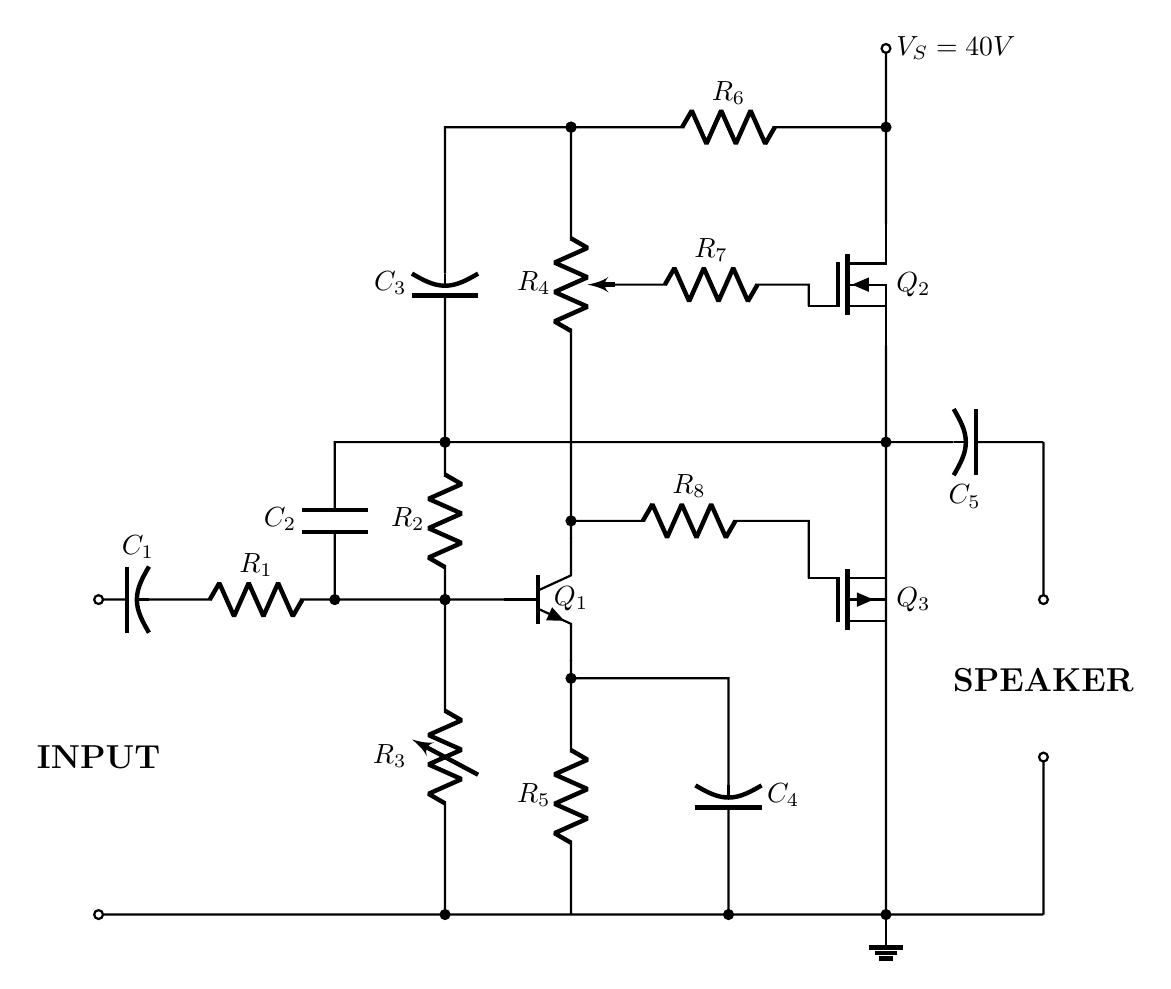
\begin{tikzpicture}[scale=2]
  \draw[color=black, thick]
    (0,0) to [short,o-] (6,0){} % Baseline for connection to ground
    % Input and ground
    (0,1) node[]{\large{\textbf{INPUT}}}
    % Connection of passive components
    (5,0) node[ground]{} node[circ](4.5,0){}
    (0,2) to [cC, l=$C_1$, o-] (0.5,2)
    to [R,l=$R_1$,](1.5,2)
    to node[short]{}(2.6,2)
    (1.5,2) to [C, l=$C_2$, *-] (1.5,3) -| (5,3)
    (2.2,2) to [R, l=$R_2$, *-*] (2.2,3)
    (2.2,3) to [cC, l=$C_3$, *-] (2.2,5) -| (3,5)
    % Transistor Bipolar Q1
    (3,0) to [R,l=$R_5$,-*] (3,1.5)
    to [Tnpn,n=npn1] (3,2.5)
    (npn1.E) node[right=3mm, above=5mm]{$Q_1$} % Labelling the NPN transistor
    (4,0) to [cC, l_=$C_4$, *-] (4, 1.5)--(3,1.5)
    (2.2,0) to [vR, l=$R_3$, *-*] (2.2,2)
    (3,2.5) to node[short]{}(3,3)
    (3,5) to [pR, n=pot1, l_=$R_4$, *-] (3,3)
    (3,5) to [R, l=$R_6$, *-] (5,5)
    to [short,*-o](5,5.5) node[right]{$V_S=40 V$}
    % Mosfet Transistors
    (5,3) to [Tnigfetd,n=mos1] (5,5)
    (mos1.B) node[anchor=west]{$Q_2$} % Labelling MOSFET Q2 Transistor
    (pot1.wiper) to [R, l=$R_7$] (4.5,4) -| (mos1.G)
    (5,1.5) to [Tpigfetd,n=mos2] (5,2.5)
    (5,0) to (mos2.S)
    (3,2.5) to [R, l=$R_8$, *-] (4.5,2.5)
    -| (mos2.G)
    (mos2.B) node[anchor=west]{$Q_3$} % Labelling MOSFET Q3 Transistor
    % Output
    (6,3) to [cC, l=$C_5$,-*](5,3)
    (6,3) to [short,-o] (6,2){}
    (mos1.S)--(mos2.D)
    (6,0) to [short,-o] (6,1){} node[above=7mm]{\large{\textbf{SPEAKER}}}
    ;
\end{tikzpicture}
\end{VerbatimOut}

\MyIO


\begin{VerbatimOut}{z.out}


\section{Kalman Filter System Model}

This Kalman filter system model was done by Burkart Lingner
\cite{lingner2010}.
\ix{Lingner, Burkart}

% An example using TikZ/PGF 2.00
%
% Features: Decorations, Fit, Layers, Matrices, Styles
% Tags: Block diagrams, Diagrams
% Technical area: Electrical engineering

%%%% \documentclass[a4paper,10pt]{article}
%%%% 
%%%% \usepackage[english]{babel}
%%%% \usepackage[T1]{fontenc}
%%%% \usepackage[ansinew]{inputenc}
%%%% 
%%%% \usepackage{lmodern}	% font definition
%%%% \usepackage{amsmath}	% math fonts
%%%% \usepackage{amsthm}
%%%% \usepackage{amsfonts}
%%%% 
%%%% \usepackage{tikz}
%%%% 
%%%% %%%<
%%%% \usepackage{verbatim}
%%%% \usepackage[active,tightpage]{preview}
%%%% \PreviewEnvironment{tikzpicture}
%%%% \setlength\PreviewBorder{5pt}%
%%%% %%%>
%%%% 
%%%% \begin{comment}
%%%% :Title: Kalman Filter System Model
%%%% :Slug: kalman-filter
%%%% :Author: Burkart Lingner
%%%% 
%%%% This is the system model of the (linear) Kalman filter. 
%%%% 
%%%% \end{comment}
%%%% 
%%%% 

\begin{figure}[htbp]
\caption{Kalman filter system model}
\centering
% The state vector is represented by a blue circle.
% "minimum size" makes sure all circles have the same size
% independently of their contents.
\tikzstyle{state}=[circle,
                                    thick,
                                    minimum size=1.2cm,
                                    draw=blue!80,
                                    fill=blue!20]

% The measurement vector is represented by an orange circle.
\tikzstyle{measurement}=[circle,
                                                thick,
                                                minimum size=1.2cm,
                                                draw=orange!80,
                                                fill=orange!25]

% The control input vector is represented by a purple circle.
\tikzstyle{input}=[circle,
                                    thick,
                                    minimum size=1.2cm,
                                    draw=purple!80,
                                    fill=purple!20]

% The input, state transition, and measurement matrices
% are represented by gray squares.
% They have a smaller minimal size for aesthetic reasons.
\tikzstyle{matrx}=[rectangle,
                                    thick,
                                    minimum size=1cm,
                                    draw=gray!80,
                                    fill=gray!20]

% The system and measurement noise are represented by yellow
% circles with a "noisy" uneven circumference.
% This requires the TikZ library "decorations.pathmorphing".
\tikzstyle{noise}=[circle,
                                    thick,
                                    minimum size=1.2cm,
                                    draw=yellow!85!black,
                                    fill=yellow!40,
                                    decorate,
                                    decoration={random steps,
                                                            segment length=2pt,
                                                            amplitude=2pt}]

% Everything is drawn on underlying gray rectangles with
% rounded corners.
\tikzstyle{background}=[rectangle,
                                                fill=gray!10,
                                                inner sep=0.2cm,
                                                rounded corners=5mm]

\begin{tikzpicture}[>=latex,text height=1.5ex,text depth=0.25ex]
    % "text height" and "text depth" are required to vertically
    % align the labels with and without indices.
  
  % The various elements are conveniently placed using a matrix:
  \matrix[row sep=0.5cm,column sep=0.5cm] {
    % First line: Control input
    &
        \node (u_k-1) [input]{$\mathbf{u}_{k-1}$}; &
        &
        \node (u_k)   [input]{$\mathbf{u}_k$};     &
        &
        \node (u_k+1) [input]{$\mathbf{u}_{k+1}$}; &
        \\
        % Second line: System noise & input matrix
        \node (w_k-1) [noise] {$\mathbf{w}_{k-1}$}; &
        \node (B_k-1) [matrx] {$\mathbf{B}$};       &
        \node (w_k)   [noise] {$\mathbf{w}_k$};     &
        \node (B_k)   [matrx] {$\mathbf{B}$};       &
        \node (w_k+1) [noise] {$\mathbf{w}_{k+1}$}; &
        \node (B_k+1) [matrx] {$\mathbf{B}$};       &
        \\
        % Third line: State & state transition matrix
        \node (A_k-2)         {$\cdots$};           &
        \node (x_k-1) [state] {$\mathbf{x}_{k-1}$}; &
        \node (A_k-1) [matrx] {$\mathbf{A}$};       &
        \node (x_k)   [state] {$\mathbf{x}_k$};     &
        \node (A_k)   [matrx] {$\mathbf{A}$};       &
        \node (x_k+1) [state] {$\mathbf{x}_{k+1}$}; &
        \node (A_k+1)         {$\cdots$};           \\
        % Fourth line: Measurement noise & measurement matrix
        \node (v_k-1) [noise] {$\mathbf{v}_{k-1}$}; &
        \node (H_k-1) [matrx] {$\mathbf{H}$};       &
        \node (v_k)   [noise] {$\mathbf{v}_k$};     &
        \node (H_k)   [matrx] {$\mathbf{H}$};       &
        \node (v_k+1) [noise] {$\mathbf{v}_{k+1}$}; &
        \node (H_k+1) [matrx] {$\mathbf{H}$};       &
        \\
        % Fifth line: Measurement
        &
        \node (z_k-1) [measurement] {$\mathbf{z}_{k-1}$}; &
        &
        \node (z_k)   [measurement] {$\mathbf{z}_k$};     &
        &
        \node (z_k+1) [measurement] {$\mathbf{z}_{k+1}$}; &
        \\
    };
    
    % The diagram elements are now connected through arrows:
    \path[->]
        (A_k-2) edge[thick] (x_k-1)	% The main path between the
        (x_k-1) edge[thick] (A_k-1)	% states via the state
        (A_k-1) edge[thick] (x_k)		% transition matrices is
        (x_k)   edge[thick] (A_k)		% accentuated.
        (A_k)   edge[thick] (x_k+1)	% x -> A -> x -> A -> ...
        (x_k+1) edge[thick] (A_k+1)
        
        (x_k-1) edge (H_k-1)				% Output path x -> H -> z
        (H_k-1) edge (z_k-1)
        (x_k)   edge (H_k)
        (H_k)   edge (z_k)
        (x_k+1) edge (H_k+1)
        (H_k+1) edge (z_k+1)
        
        (v_k-1) edge (z_k-1)				% Output noise v -> z
        (v_k)   edge (z_k)
        (v_k+1) edge (z_k+1)
        
        (w_k-1) edge (x_k-1)				% System noise w -> x
        (w_k)   edge (x_k)
        (w_k+1) edge (x_k+1)
        
        (u_k-1) edge (B_k-1)				% Input path u -> B -> x
        (B_k-1) edge (x_k-1)
        (u_k)   edge (B_k)
        (B_k)   edge (x_k)
        (u_k+1) edge (B_k+1)
        (B_k+1) edge (x_k+1)
        ;
    
    % Now that the diagram has been drawn, background rectangles
    % can be fitted to its elements. This requires the TikZ
    % libraries "fit" and "background".
    % Control input and measurement are labeled. These labels have
    % not been translated to English as "Measurement" instead of
    % "Messung" would not look good due to it being too long a word.
    \begin{pgfonlayer}{background}
        \node [background,
                    fit=(u_k-1) (u_k+1),
                    label=left:Entrance:] {};
        \node [background,
                    fit=(w_k-1) (v_k-1) (A_k+1)] {};
        \node [background,
                    fit=(z_k-1) (z_k+1),
                    label=left:Measure:] {};
    \end{pgfonlayer}
\end{tikzpicture}

\end{figure}
\end{VerbatimOut}

\MyIO


  % Linguistics.
  %\ProvidesFile{ap-linguistics.tex}[2022-10-05 linguistics appendix]

\begin{VerbatimOut}{z.out}
\chapter{LINGUISTICS}
\ix{linguistics//Linguistics appendix}

See WIKIBOOKS \LaTeX/Linguistics \cite{wikibooks-latex-linguistics}
or google for the information you need.

The doulossil font
\cite{tambe2020}
is a TrueType font.
Version 0.1 on September 21, 2020 claimed
``it has characters that are not in other TeX IPA fonts''.
\end{VerbatimOut}

\MyIO


\begin{VerbatimOut}{z.out}


\section{Demonstrate the example and examples environments}

The example and examples environment
are defined
in the covington
\cite{covington2021}
package.

Demonstrate the example environment:
\begin{example}
  This is an example.
  This is an example.
\end{example}

Demonstrate the examples environment:
\begin{examples}
  \item First example.
  \item Second example.
\end{examples}
\end{VerbatimOut}

\MyIO


  % Mathematics.
  %\ProvidesFile{ap-mathematics.tex}[2022-10-05 mathematics appendix]

\begin{VerbatimOut}{z.out}
\chapter{MATHEMATICS}
\ix{mathematics//Mathematics appendix}

\PurdueThesisLogo\ loads the \AMSmathLogo\ package
\cite{amslatex3project2019}
to do mathematics.
\end{VerbatimOut}


\subsection{Photoswitching induced spatial coherence}

Photoswitching fluorescent molecules are described in the density matrix formalism

\begin{equation*}
\rho = \xi\ket{\alpha}\bra{\alpha} + (1-\xi)\ket{0}\bra{0}
\end{equation*}

where $\ket{\alpha}$ is a coherent state with amplitude $\alpha$ i.e., $\langle n\rangle = \bra{\alpha} n\ket{\alpha} = |\alpha|^{2}$. We consider a simplified model consisting of a single mode field 

\begin{equation*}
E_{0}^{+}\sim \sum_{j=1}^{M}\delta(s-s_{j})a_{j} \;\; E^{+}(r_{i}) = \int d^{2}s E_{0}^{+} h(r-s) = h(r_{i}-s)\hat{a}
\end{equation*}

\begin{equation*}
g^{(2)}_{ij}(0) = \frac{\langle E^{-}(r_{i})E^{-}(r_{j})E^{+}(r_{i})E^{+}(r_{j}) \rangle}{\langle E^{-}(r_{i})E^{+}(r_{i})\rangle\langle E^{-}(r_{j})E^{+}(r_{j})\rangle} = \frac{\mathrm{Tr}(a^{\dagger}a^{\dagger}aa\rho)}{\mathrm{Tr}(a^{\dagger}a\rho)^{2}}
\end{equation*}

Notice that terms related to point spread function will cancel. Now,

\begin{align*}
\mathrm{Tr}(a^{\dagger}a^{\dagger}aa\rho) &= \mathrm{Tr}(a^{\dagger}a^{\dagger}aa \left(\xi\ket{\alpha}\bra{\alpha} + (1-\xi)\ket{0}\bra{0}\right))\\
&= \mathrm{Tr}\left(\xi e^{-|\alpha|^{2}}\sum_{n,m}^{\infty}\frac{\alpha^{n}}{n!}\ket{n}\bra{m}\right)\\
&= \mathrm{Tr}\left(\xi e^{-|\alpha|^{2}}\sum_{n}^{\infty}\frac{|\alpha|^{2n}}{n!}n(n-1)\right)\\
&= \mathrm{Tr}\left(\xi e^{-|\alpha|^{2}}\sum_{n=2}^{\infty}\frac{|\alpha|^{2n}}{(n-2)!}\right)\\
&= \xi|\alpha|^{4}
\end{align*}

The second trace in the denominator proceeds similarly to the first

\begin{align*}
\mathrm{Tr}(a^{\dagger}a\rho) &= \mathrm{Tr}(a^{\dagger}a \left(\xi\ket{\alpha}\bra{\alpha} + (1-\xi)\ket{0}\bra{0}\right))\\
&= \mathrm{Tr}\left(\xi e^{-|\alpha|^{2}}\sum_{n,m}^{\infty}\frac{\alpha^{n}}{n!}\ket{n}\bra{m} \right)\\
&= \mathrm{Tr}\left(\xi e^{-|\alpha|^{2}}\sum_{n}^{\infty}\frac{|\alpha|^{2n}}{n!}n\right)\\
&= \mathrm{Tr}\left(\xi e^{-|\alpha|^{2}}\sum_{n=2}^{\infty}\frac{|\alpha|^{2n}}{(n-1)!}\right)\\
&= \xi|\alpha|^{2}
\end{align*}

As expected, this gives $\langle n\rangle$. Putting it all together yields a simple expression for the two-point coherence function

\begin{equation*}
g^{(2)}_{ij}(0) = \frac{\xi|\alpha|^{4}}{\xi^{2}|\alpha|^{4}} = \frac{1}{\xi}
\end{equation*}

Notice that as $\xi\rightarrow 1$ (always on) we recover the coherent state. As $\xi\rightarrow 0$ we observe $g^{(2)}_{ij}(0) > 1$ i.e., bunching. This is a critical result: photoswitching results in non-trivial correlations between pixels $i$ and $j$. Introducing more than one photoswitching emitter gives? In practice, we can estimate of $g^{(2)}_{ij}(0)$ in a finite time interval. I guess that $\langle n_{i}\rangle = \xi |\alpha|^{2}\Delta = 0.5$ is reasonable; however this is best addressed by Monte Carlo simulation. The total interval $T$ constrained by the super-resolution frame rate e.g., $T=10\mathrm{ms}$. 



\subsection{Details of the Gaussian PSF}

We will derive the gradients for the integrated astigmatic Gaussian, since it is the more general case. As before, define $i_{0} = g_{k}\gamma\Delta t N_{0}$ such that $\mu_{k}' = i_{0}\lambda_{k}$

\begin{equation*}
J_{x_{0}} = \beta_{k}\lambda_{y}\frac{\partial \lambda_{x}}{\partial x_{0}} \;\; J_{y_{0}} = \beta_{k}\lambda_{x}\frac{\partial \lambda_{y}}{\partial y_{0}}\;\;\; J_{z_{0}}  = \frac{\partial \mu_{k}'}{\partial \sigma_{x}}\frac{\partial \sigma_{x}}{\partial z_{0}} + \frac{\partial \mu_{k}'}{\partial \sigma_{y}}\frac{\partial \sigma_{y}}{\partial z_{0}}
\end{equation*}

\begin{align*}
J_{x_{0}} &= \beta_{k}\lambda_{y}\frac{\partial \lambda_{x}}{\partial x_{0}} \\
&= \frac{\beta_{k}\lambda_{y}}{2}\frac{\partial}{\partial x_{0}}\left(\mathrm{erf}\left(\frac{x_{k}+\frac{1}{2}-x_{0}}{\sqrt{2}\sigma_{x}}\right) -\mathrm{erf}\left(\frac{x_{k}-\frac{1}{2}-x_{0}}{\sqrt{2}\sigma_{x}}\right)\right)\\
&= \frac{\beta_{k}\lambda_{y}}{\sqrt{2\pi}\sigma_{x}}\left(\mathrm{exp}\left(\frac{(x_{k}-\frac{1}{2}-x_{0})^{2}}{2\sigma_{x}^{2}}\right) -\mathrm{exp}\left(\frac{(x_{k}+\frac{1}{2}-x_{0})^{2}}{2\sigma_{x}^{2}}\right)\right)
\end{align*}

\begin{align*}
J_{y_{0}} &= \beta_{k}\lambda_{x}\frac{\partial \lambda_{y}}{\partial y_{0}} \\
&= \frac{\beta_{k}\lambda_{x}}{2}\frac{\partial}{\partial y_{0}}\left(\mathrm{erf}\left(\frac{y_{k}+\frac{1}{2}-y_{0}}{\sqrt{2}\sigma_{y}}\right) -\mathrm{erf}\left(\frac{y_{k}-\frac{1}{2}-y_{0}}{\sqrt{2}\sigma_{y}}\right)\right)\\
&= \frac{\beta_{k}\lambda_{x}}{\sqrt{2\pi}\sigma_{y}}\left(\mathrm{exp}\left(\frac{(y_{k}-\frac{1}{2}-y_{0})^{2}}{2\sigma_{y}^{2}}\right) -\mathrm{exp}\left(\frac{(y_{k}+\frac{1}{2}-y_{0})^{2}}{2\sigma_{y}^{2}}\right)\right)
\end{align*}

\begin{align*}
J_{\sigma_{x}} &= \beta_{k}\lambda_{y}\frac{\partial \lambda_{x}}{\partial \sigma_{x}} \\
&= \frac{\beta_{k}\lambda_{y}}{2}\frac{\partial}{\partial \sigma_{x}}\left(\mathrm{erf}\left(\frac{x_{k}+\frac{1}{2}-x_{0}}{\sqrt{2}\sigma_{x}}\right) -\mathrm{erf}\left(\frac{x_{k}-\frac{1}{2}-x_{0}}{\sqrt{2}\sigma_{x}}\right)\right)\\
&= \frac{\beta_{k}\lambda_{y}}{\sqrt{2\pi}}\left(\frac{\left(x-x_{0}-\frac{1}{2}\right) e^{-\frac{\left(x-x_{0}-\frac{1}{2}\right)^2}{2 \sigma_{x} ^2}}}{\sigma_{x} ^2}-\frac{ \left(x-x_{0}+\frac{1}{2}\right) e^{-\frac{\left(x-x_{0}+\frac{1}{2}\right)^2}{2 \sigma_{x} ^2}}}{\sigma_{x} ^2}\right)
\end{align*}

\begin{align*}
J_{\sigma_{y}} &= \beta_{k}\lambda_{x}\frac{\partial \lambda_{y}}{\partial \sigma_{y}} \\
&= \frac{\beta_{k}\lambda_{x}}{2}\frac{\partial}{\partial \sigma_{y}}\left(\mathrm{erf}\left(\frac{y_{k}+\frac{1}{2}-y_{0}}{\sqrt{2}\sigma_{y}}\right) -\mathrm{erf}\left(\frac{y_{k}-\frac{1}{2}-y_{0}}{\sqrt{2}\sigma_{y}}\right)\right)\\
&= \frac{\beta_{k}\lambda_{x}}{\sqrt{2\pi}}\left(\frac{\left(y-y_{0}-\frac{1}{2}\right) e^{-\frac{\left(y-y_{0}-\frac{1}{2}\right)^2}{2 \sigma_{y} ^2}}}{\sigma_{y} ^2}-\frac{ \left(y-y_{0}+\frac{1}{2}\right) e^{-\frac{\left(y-y_{0}+\frac{1}{2}\right)^2}{2 \sigma_{y} ^2}}}{\sigma_{y} ^2}\right)
\end{align*}

Luckily, computing the Hessian matrix for (2.9) is tractable, and is actually quite simple when one takes advantage of the chain rule for Hessian matrices. Looking at (2.9), the likelihood is a hierarchical function that maps a vector space $\Theta$ to a vector space $\Lambda$ to a scalar value. Formally, we define $T: \Theta \rightarrow \Lambda$ and $W: \Lambda \rightarrow \mathbb{R}$. The parameter vector $(x_{0},y_{0},z_{0}, \sigma_{0}, N_{0})\in \Theta$, the Poisson rate vector $\vec{\lambda} \in \Lambda$ and $\ell \in \mathbb{R}$. Note that we choose to optimize $\sigma_{x}$ and $\sigma_{y}$ directly and compute $z_{0}$ to simplify the computation of the Hessian. To get the Hessian, we need the chain-rule for Hessian matrices, which can be quickly computed in terms of the jacobian and hessian of $T$ and $W$.


\begin{equation*}
H_{\ell} = J_{\mu}^{T} H_{\ell} J_{\mu} + (J_{\ell}\otimes I_{n})H_{\mu}
\end{equation*}

where we have used $J_{\mu}$ to represent the jacobian of $T$ and $J_{\ell}$ for the jacobian of $W$. Similar notation is used for the corresponding Hessian matrices. 
In the 3D case, the Hessian matrix is not directly separable since $\mu \propto \lambda_{x}(x_{0},\sigma_{0},\sigma_{x})\lambda_{y}(y_{0},\sigma_{0},\sigma_{y})$. To see this, an abstract representation of the Hessian reads 


\subsection{Fisher information for 2D integrated gaussian}

For the 2D integrated gaussian point spread function, the Hessian only contains separable second order derivatives, so the Fisher information matrix takes on a convenient form

\begin{equation}
I_{ij}(\theta) = \underset{\theta}{\mathbb{E}}\left(\frac{\partial \ell}{\partial\theta_{i}}\frac{\partial\ell}{\partial\theta_{j}}\right) 
\end{equation}

For an arbitrary parameter then we have

\begin{align*}
\frac{\partial \ell}{\partial \theta_{i}} &= \frac{\partial}{\partial \theta_{i}} \sum_{k}  x_{k}\log x_{k} + \mu_{k}' - x_{k}\log\left(\mu_{k}'\right)\\
&= \sum_{k} \frac{\partial \mu_{k}'}{\partial\theta_{i}} \left(\frac{\mu_{k}'-x_{k}}{\mu_{k}'}\right)
\end{align*}

\begin{equation*}
I_{ij}(\theta) = \underset{\theta}{\mathbb{E}}\left(\sum_{k}\frac{\partial \mu_{k}'}{\partial\theta_{i}}\frac{\partial \mu_{k}'}{\partial\theta_{j}} \left(\frac{\mu_{k}'-x_{k}}{\mu_{k}'}\right)^{2}\right) = \sum_{k}\frac{1}{\mu_{k}'}\frac{\partial \mu_{k}'}{\partial\theta_{i}}\frac{\partial \mu_{k}'}{\partial\theta_{j}}
\end{equation*}

To compute the bound, it turns out all we need is the jacobian $\frac{\partial \mu_{k}'}{\partial\theta_{j}} $.

\section{The Fokker-Planck Equation}

The Fokker-Planck equation is a central tool in non-equilibrium statistical mechanics, analagous to the master equation for discrete systems. It allows us to determine the time evolution of probability densities over continuous state spaces. Important examples in biophysics are the phase space of a particle or the membrane potential of a nerve cell.

Suppose we have a random variable $\bm{x}$ and its joint distribution $P(\bm{x},t)$, which is not necessarily stationary. Define a vector field $\vec{J}(\bm{x},t)$ which is the probability current, which we will specify in a moment. The Fokker-Planck equation is by starting with a continuity equation for probability 

\begin{align*}
\frac{d}{dt}\int_{V_{0}} P(\bm{x},t)dV &= \int_{S}P(\bm{x},t)(\vec{J}\cdot\hat{n})dS\\
&= -\int_{V_{0}}P(\bm{x},t)(\nabla\cdot \vec{J})dV
\end{align*}

Clearly this implies that

\begin{equation*}
\frac{dP(\bm{x},t)}{dt} = -\left(\nabla\cdot \vec{J}\right)P(\bm{x},t)
\end{equation*}

We often call the divergence term, the Fokker-Planck operator $\mathcal{L}_{FP}=-\nabla\cdot \vec{J}$. A more rigorous derivation is given in the appendix, which tells us that, to second order

\begin{equation*}
J(x_{i},t)  = \left(M_{i}^{(1)}(t) - \sum_{j}\frac{\partial}{\partial x_{j}}M_{ij}^{(2)}(t) \right)P(\bm{x},t)
\end{equation*}

where $M_{i}^{n}(t)$ is the $n$th moment of a transition kernel $T(x_{i}',t'|x_{i},t)$ for variable $i$. The first moment is essentially just the deterministic part of the Langevin dynamics. The second and higher moments will depend on these higher moments in the stochastic forcing terms. As proven more completely in the appendix, the full multi-dimensional Fokker-Planck equation reads

\begin{align}
\frac{\partial P(\vec{x},t)}{\partial t}  &= \vec{\nabla} \cdot J(\vec{x},t)\\
&= \sum_{i=1}^{N}\left(-\frac{\partial}{\partial x_{i}}M_{i}^{(1)}(t) + \sum_{j=1}^{N} \frac{\partial^{2}}{\partial x_{i}\partial x_{j}}M_{ij}^{(2)}(t)\right)P(\vec{x},t)
\end{align}

If we make a further constraint that the moments of the transition operator are stationary $M_{i}^{(1)}(t) = \Upsilon_{ij}$ and $M_{ij}^{(2)}(t) = D_{ij}$ 

\begin{align}
\frac{\partial P(\vec{x},t)}{\partial t}  &= \sum_{ij}\left(\Upsilon_{ij}\frac{\partial}{\partial x_{i}} + D_{ij}\frac{\partial^{2}}{\partial x_{i}\partial x_{j}}\right)P(\vec{x},t)
\end{align}

\begin{equation*}
D = \begin{pmatrix}0&0 \\ 0& \gamma k_{B}T/m \end{pmatrix}\;\;\Upsilon = \begin{pmatrix}0 & -1\\ 0 & \gamma\end{pmatrix}
\end{equation*}

\section{Free Brownian particle}

Consider a familiar Langevin dynamics on phase space $\bm{x} = (x,v)$, where a free particle ($V(x)=0\; \forall x$) experiences a viscous drag force and stochastic forcing $\xi(t)$ where $\xi(t)\sim\mathcal{N}(\mu,\sigma^{2})$ and $\langle \xi(t)\xi(t+\tau)\rangle = \delta(t-\tau)$. 

\begin{align*}
\dot{x} &= v\\
\dot{v} &= -\frac{\gamma}{m}v + \frac{1}{m}\xi(t)
\end{align*}

The moments of the transition kernel must be

\begin{equation*}
M_{x}^{(1)} = v  \;\; M_{v}^{(1)} = -\frac{\gamma}{m}v + \mu \;\; M_{v}^{(v)} = \sigma^{2}
\end{equation*}

To simplify the notation let us define $\nabla\cdot \vec{J} = \frac{\partial J_{x}}{\partial x} + \frac{\partial J_{x}}{\partial v}= \mathcal{L}_{x} + \mathcal{L}_{v} = \mathcal{L}_{FP}$. This gives the full Fokker-Planck equation $\frac{dP(\bm{x},t)}{dt} = -\mathcal{L}_{FP}P(\bm{x},t)$. 

\begin{align*}
\mathcal{L}_{x}P(\bm{x},t) &= \frac{\partial}{\partial x}\left(vP(\bm{x},t)\right)\\
\mathcal{L}_{v}P(\bm{x},t) &= \frac{\partial}{\partial v}\left(-\frac{\gamma}{m}v + \frac{1}{m}F(x)\right)P(\bm{x},t) + \sigma^{2}\frac{\partial^{2}}{\partial v^{2}}P(\bm{x},t)
\end{align*}


\section{The Brownian Harmonic oscillator}

Consider a familiar Langevin dynamics on phase space $\bm{x} = (x,v)$, where a particle in a potential $V(x)$ experiences a viscous drag force and stochastic forcing $\xi(t)$ where $\xi(t)\sim\mathcal{N}(\mu,\sigma^{2})$ and $\langle \xi(t)\xi(t+\tau)\rangle = \delta(t-\tau)$. 

\begin{align*}
\dot{x} &= v\\
\dot{v} &= -\frac{\gamma}{m}v + \frac{1}{m}F(x) + \frac{1}{m}\xi(t)
\end{align*}

The moments of the transition kernel must be

\begin{equation*}
M_{x}^{(1)} = v  \;\; M_{v}^{(1)} = -\frac{\gamma}{m}v + \frac{1}{m}F(x) + \mu \;\; M_{v}^{(v)} = \sigma^{2}
\end{equation*}

To simplify the notation let us define $\nabla\cdot \vec{J} = \frac{\partial J_{x}}{\partial x} + \frac{\partial J_{x}}{\partial v}= \mathcal{L}_{x} + \mathcal{L}_{v} = \mathcal{L}_{FP}$. This gives the full Fokker-Planck equation $\frac{dP(\bm{x},t)}{dt} = -\mathcal{L}_{FP}P(\bm{x},t)$. 

\begin{align*}
\mathcal{L}_{x}P(\bm{x},t) &= \frac{\partial}{\partial x}\left(vP(\bm{x},t)\right)\\
\mathcal{L}_{v}P(\bm{x},t) &= \frac{\partial}{\partial v}\left(-\frac{\gamma}{m}v + \frac{1}{m}F(x)\right)P(\bm{x},t) + \sigma^{2}\frac{\partial^{2}}{\partial v^{2}}P(\bm{x},t)
\end{align*}


  % Music.
  %\ProvidesFile{ap-music.tex}[2022-10-05 music appendix]

\begin{VerbatimOut}{z.out}
\chapter{MUSIC}
\ix{music//Music appendix}

To get the following printed music score I did the following steps.
\begin{itemize}
  \item
    Get the ``Example of LilyPond input file''
    from the Wikipedia LilyPond page
    \cite{wikipedia-lilypond}
    and put it in a \verb+fib.ly+ file.
  \item
    Ran \verb+lilypond fib.ly+ and got the following \verb+fib.pdf+ file:
\end{itemize}
\ix{LilyPond music typesetting software}

\noindent \includegraphics[scale=0.77]{gr-fib.pdf}
\end{VerbatimOut}

\MyIO


  % The examples in ap-physics require LuaLaTeX but LuaLaTeX
  % screws up the spacing in the List of Figures.  So, the
  % ap-physics file is not included.
  %
  % For some reason, ap-physics doesn't work when using BibTeX.
  % Just enclosing \ProvidesFile{ap-physics.tex}[2022-10-05 Physics appendix]

\chapter{Optical fluctuation microscopy}
\ix{physics//Physics appendix}

\subsection{Spatial coherence for an isolated emitter}

Photoswitching fluorescent molecules are described in the density matrix formalism

\begin{equation*}
\rho = \sum_{k}\xi_{k}\ket{\alpha_{k}}\bra{\alpha_{k}}\;\; \sum_{k}\xi_{k} = 1
\end{equation*}


where $\ket{\alpha_{k}}$ is a coherent state with amplitude $\alpha_{k}$ i.e., $\langle n\rangle = \bra{\alpha_{k}} n\ket{\alpha_{k}} = \lvert\alpha_{k}^{2}\rvert$. Typically $\xi_{k}$ and $\langle n_{k}\rangle$ are heterogeneous. We consider a simplified model consisting of a single mode field 

\begin{equation*}
E^{+}(r_{i}) = h(r_{i}-s_{0})\hat{a}_{n}
\end{equation*}

\begin{equation*}
g^{(2)}_{ij}(0) = \frac{\langle E^{-}(r_{i})E^{-}(r_{j})E^{+}(r_{i})E^{+}(r_{j}) \rangle}{\langle E^{-}(r_{i})E^{+}(r_{i})\rangle\langle E^{-}(r_{j})E^{+}(r_{j})\rangle} = \frac{\mathrm{Tr}(E^{-}(r_{i})E^{-}(r_{j})E^{+}(r_{i})E^{+}(r_{j})\rho)}{\mathrm{Tr}(E^{-}(r_{i})E^{+}(r_{i})\rho)\mathrm{Tr}(E^{-}(r_{j})E^{+}(r_{j})\rho)}
\end{equation*}

Terms related to point spread function will cancel. It is instructive to compute

\begin{align*}
\mathrm{Tr}(a^{\dagger}a^{\dagger}aa \left(\xi_{k}\ket{\alpha_{k}}\bra{\alpha_{k}}\right) &= \mathrm{Tr}\left(\xi_{k} e^{-\lvert\alpha\rvert^{2}}\sum_{n,m}^{\infty}\frac{\alpha^{n}}{n!}\ket{n}\bra{m}\right)\\
&= \mathrm{Tr}\left(\xi_{k} e^{-\lvert\alpha\rvert^{2}}\sum_{n}^{\infty}\frac{\lvert\alpha\rvert^{2n}}{n!}n(n-1)\right)\\
&= \mathrm{Tr}\left(\xi_{k} e^{-\lvert\alpha\rvert^{2}}\sum_{n=2}^{\infty}\frac{\lvert\alpha\rvert^{2n}}{(n-2)!}\right)\\
&= \xi_{k}\lvert\alpha_{k}\rvert^{4}
\end{align*}

Similarly,

\begin{align*}
\mathrm{Tr}(a^{\dagger}a \left(\xi \ket{\alpha}\bra{\alpha}\right)) &= \mathrm{Tr}\left(\xi e^{-\lvert\alpha\rvert^{2}}\sum_{n,m}^{\infty}\frac{\alpha^{n}(\alpha^{m})^{*}}{\sqrt{n!}\sqrt{m!}}a^{\dagger}a\ket{n}\bra{m} \right)\\
&= \xi e^{-\lvert\alpha\rvert^{2}}\sum_{n=0}^{\infty}\frac{(\lvert\alpha\rvert^{2})^{n}}{n!}n\\
&= \xi e^{-\lvert\alpha\rvert^{2}}\sum_{n=1}^{\infty}\frac{(\lvert\alpha\rvert^{2})^{n}}{(n-1)!}\\
&= \xi e^{-\lvert\alpha\rvert^{2}}\left(\lvert\alpha\rvert^{2} + \frac{\lvert\alpha\rvert^{4}}{1!} + \frac{\lvert\alpha\rvert^{6}}{2!}+...\right)\\
&= \xi e^{-\lvert\alpha\rvert^{2}}\lvert\alpha\rvert^{2}\left(1 + \frac{\lvert\alpha\rvert^{2}}{1!} + \frac{\lvert\alpha\rvert^{3}}{2!}+...\right)\\
&= \xi e^{-\lvert\alpha\rvert^{2}}e^{\lvert\alpha\rvert^{2}}\lvert\alpha\rvert^{2} = \xi\lvert\alpha\rvert^{2}
\end{align*}

\begin{align*}
\mathrm{Tr}(a a^{\dagger} \left(\xi \ket{\alpha}\bra{\alpha}\right)) &= \mathrm{Tr}\left(\xi e^{-\lvert\alpha\rvert^{2}}\sum_{n,m}^{\infty}\frac{\alpha^{n}(\alpha^{m})^{*}}{\sqrt{n!}\sqrt{m!}}a a^{\dagger}\ket{n}\bra{m} \right)\\
&= \xi e^{-\lvert\alpha\rvert^{2}}\sum_{n=0}^{\infty}\frac{(\lvert\alpha\rvert^{2})^{n}}{n!}(n+1)\\
&= \xi e^{-\lvert\alpha\rvert^{2}}\left(\sum_{n=1}^{\infty}\frac{(\lvert\alpha\rvert^{2})^{n}}{(n-1)!} + e^{\lvert\alpha\rvert^{2}}\right)\\
&= \xi e^{-\lvert\alpha\rvert^{2}}\left(\lvert\alpha\rvert^{2}e^{\lvert\alpha\rvert^{2}} + e^{\lvert\alpha\rvert^{2}}\right) = \xi(\lvert\alpha\rvert^{2} + 1)
\end{align*}

Putting it all together yields a simple expression for the two-point coherence function

\begin{equation*}
g^{(2)}_{ij}(0) = \frac{\sum_{k}\xi_{k}\lvert\alpha_{k}\rvert^{4}}{\left(\sum_{k}\xi_{k}\lvert\alpha_{k}\rvert^{2}\right)\left(\sum_{k}\xi_{k}\lvert\alpha_{k}\rvert^{2}\right)}
\end{equation*}

For example, if we have a two-level system consisting of a fluorescent state with amplitude $\alpha$ and the vacuum state, this becomes

\begin{equation*}
g^{(2)}_{ij}(0) = \frac{\xi\lvert\alpha\rvert^{4}}{\xi^{2}\lvert\alpha\rvert^{4}} = \frac{1}{\xi}
\end{equation*}

As $\xi\rightarrow 1$ (always on) we recover a coherent state. As $\xi\rightarrow 0$ we observe $g^{(2)}_{ij}(0) > 1$ i.e., bunching.

\subsection{Generalization to nonzero background}

\begin{equation*}
E_{0}^{+}\sim \sum_{j=1}^{M}\delta(s-s_{j})a_{j} \;\; E^{+}(r_{i}) = \int d^{2}s E_{0}^{+} = \sum_{n}h(r_{i}-s_{n})a_{n}
\end{equation*}

\begin{equation*}
\rho_{S} = \xi\ket{\alpha}\bra{\alpha} + (1-\xi)\ket{0}\bra{0}\;\;\rho_{B} = \ket{\beta}\bra{\beta}\;\;\rho = \rho_{S}\otimes\rho_{B}
\end{equation*}

\begin{equation*}
E(r_{i})^{+} = E_{S}(r_{i})^{+} + E_{B}(r_{i})^{+} = h(r_{i}-s_{n})a_{S} + a_{B}
\end{equation*}

\begin{align*}
G^{2}_{ij}(0) &= \langle(E_{S}^{\dagger} + E_{B}^{\dagger}) (E_{S}^{\dagger} + E_{B}^{\dagger})( E_{S} + E_{B}) (E_{S} + E_{B})\rangle \\
&= h_{i}^{2}h_{j}^{2}\langle a_{S}^{\dagger}a_{S}^{\dagger}a_{S}a_{S}\rangle + h_{i}^{2}\langle a_{S}^{\dagger}a_{B}^{\dagger}a_{S}a_{B}\rangle + h_{j}^{2}\langle a_{B}^{\dagger}a_{S}^{\dagger}a_{B}a_{S}\rangle  + \langle a_{B}^{\dagger}a_{B}^{\dagger}a_{B}a_{B}\rangle  \\
&= \xi(h_{i}^{2}h_{j}^{2}\lvert\alpha\rvert^{4}+ h_{i}^{2}\lvert\alpha\rvert^{2}\lvert\beta\rvert^{2} + h_{j}^{2}\lvert\alpha\rvert^{2}\lvert\beta\rvert^{2}\rangle  + \lvert\beta\rvert^{4} ) \\
&= \xi(h_{i}^{2}h_{j}^{2}\lvert\alpha\rvert^{4}+ \lvert\alpha\rvert^{2}\lvert\beta\rvert^{2}(h_{i}^{2} + h_{j}^{2})  + \lvert\beta\rvert^{4}) \\
\end{align*}

The normalized second order coherence function then reads

\begin{align*}
g^{2}_{ij}(0) &= \frac{\xi h_{i}^{2}h_{j}^{2}N_{0}^{2} + \xi N_{0}B_{0}(h_{i}^{2} + h_{j}^{2}) + B_{0}^{2}}{\xi^{2} h_{i}^{2}h_{j}^{2}N_{0}^{2} + \xi N_{0}B_{0}(h_{i}^{2}+h_{j}^{2}) +  B_{0}^{2}}
\end{align*}

Notice the PSF factor $h_{i}$ appears squared. This squared value can be seen as the probability of photon detection at a point $s_i$, while $h_{i}$ is the amplitude of the electric field. 

\subsection{Ergodicity of photoswitching}

In general, Markov jump processes are non-ergodic, meaning that their time averages and ensemble averages are not equal. The use of $\xi$ as a probability is only valid when the observation duration (exposure time) is much longer than the characteristic switching time. However, the use of $\xi$ above is quite convenient, so we look to determine how long our exposure must be for the emitter to be considered in equilibrium. For a two state process

\begin{equation*}
P(t) = e^{Wt}P(0)\rightarrow \dot{P}(t) = We^{Wt}P(0)
\end{equation*}

\begin{equation*}
e^{Wt} = I + W\frac{1-e^{-2\lambda t}}{2\lambda}
\end{equation*}

where $\lambda = (\lambda_1 + \lambda_2)/2$. Now,

\begin{equation*}
\dot{P}(t) = W\left(I + W\frac{1-e^{-2\lambda t}}{2\lambda}\right)P(0)
\end{equation*}

It can then be shown that the individual gradients are


\begin{equation*}
\begin{pmatrix}
\frac{\lambda_1 \lambda_2 \left(1-e^{-t (\lambda_1+\lambda_2)}\right)}{\lambda_1+\lambda_2}-\lambda_1 \left(1-\frac{\lambda_1 \left(1-e^{-t (\lambda_1+\lambda_2)}\right)}{\lambda_1+\lambda_2}\right) & \lambda_2 \left(1-\frac{\lambda_2 \left(1-e^{-t (\lambda_1+\lambda_2)}\right)}{\lambda_1+\lambda_2}\right)-\frac{\lambda_1 \lambda_2 \left(1-e^{-t (\lambda_1+\lambda_2)}\right)}{\lambda_1+\lambda_2} \\
\lambda_1 \left(1-\frac{\lambda_1 \left(1-e^{-t (\lambda_1+\lambda_2)}\right)}{\lambda_1+\lambda_2}\right)-\frac{\lambda_1 \lambda_2 \left(1-e^{-t (\lambda_1+\lambda_2)}\right)}{\lambda_1+\lambda_2} & \frac{\lambda_1 \lambda_2 \left(1-e^{-t (\lambda_1+\lambda_2)}\right)}{\lambda_1+\lambda_2}-\lambda_2 \left(1-\frac{\lambda_2 \left(1-e^{-t (\lambda_1+\lambda_2)}\right)}{\lambda_1+\lambda_2}\right)
\end{pmatrix}
\end{equation*}



\subsection{Details of the Gaussian PSF}\

We will derive the gradients for the integrated astigmatic Gaussian, since it is the more general case. As before, define $i_{0} = g_{k}\gamma\Delta t N_{0}$ such that $\mu_{k}' = i_{0}\lambda_{k}$

\begin{equation*}
J_{x_{0}} = \beta_{k}\lambda_{y}\frac{\partial \lambda_{x}}{\partial x_{0}} \;\; J_{y_{0}} = \beta_{k}\lambda_{x}\frac{\partial \lambda_{y}}{\partial y_{0}}\;\;\; J_{z_{0}}  = \frac{\partial \mu_{k}'}{\partial \sigma_{x}}\frac{\partial \sigma_{x}}{\partial z_{0}} + \frac{\partial \mu_{k}'}{\partial \sigma_{y}}\frac{\partial \sigma_{y}}{\partial z_{0}}
\end{equation*}

\begin{align*}
J_{x_{0}} &= \beta_{k}\lambda_{y}\frac{\partial \lambda_{x}}{\partial x_{0}} \\
&= \frac{\beta_{k}\lambda_{y}}{2}\frac{\partial}{\partial x_{0}}\left(\mathrm{erf}\left(\frac{x_{k}+\frac{1}{2}-x_{0}}{\sqrt{2}\sigma_{x}}\right) -\mathrm{erf}\left(\frac{x_{k}-\frac{1}{2}-x_{0}}{\sqrt{2}\sigma_{x}}\right)\right)\\
&= \frac{\beta_{k}\lambda_{y}}{\sqrt{2\pi}\sigma_{x}}\left(\mathrm{exp}\left(\frac{(x_{k}-\frac{1}{2}-x_{0})^{2}}{2\sigma_{x}^{2}}\right) -\mathrm{exp}\left(\frac{(x_{k}+\frac{1}{2}-x_{0})^{2}}{2\sigma_{x}^{2}}\right)\right)
\end{align*}

\begin{align*}
J_{y_{0}} &= \beta_{k}\lambda_{x}\frac{\partial \lambda_{y}}{\partial y_{0}} \\
&= \frac{\beta_{k}\lambda_{x}}{2}\frac{\partial}{\partial y_{0}}\left(\mathrm{erf}\left(\frac{y_{k}+\frac{1}{2}-y_{0}}{\sqrt{2}\sigma_{y}}\right) -\mathrm{erf}\left(\frac{y_{k}-\frac{1}{2}-y_{0}}{\sqrt{2}\sigma_{y}}\right)\right)\\
&= \frac{\beta_{k}\lambda_{x}}{\sqrt{2\pi}\sigma_{y}}\left(\mathrm{exp}\left(\frac{(y_{k}-\frac{1}{2}-y_{0})^{2}}{2\sigma_{y}^{2}}\right) -\mathrm{exp}\left(\frac{(y_{k}+\frac{1}{2}-y_{0})^{2}}{2\sigma_{y}^{2}}\right)\right)
\end{align*}

\begin{align*}
J_{\sigma_{x}} &= \beta_{k}\lambda_{y}\frac{\partial \lambda_{x}}{\partial \sigma_{x}} \\
&= \frac{\beta_{k}\lambda_{y}}{2}\frac{\partial}{\partial \sigma_{x}}\left(\mathrm{erf}\left(\frac{x_{k}+\frac{1}{2}-x_{0}}{\sqrt{2}\sigma_{x}}\right) -\mathrm{erf}\left(\frac{x_{k}-\frac{1}{2}-x_{0}}{\sqrt{2}\sigma_{x}}\right)\right)\\
&= \frac{\beta_{k}\lambda_{y}}{\sqrt{2\pi}}\left(\frac{\left(x-x_{0}-\frac{1}{2}\right) e^{-\frac{\left(x-x_{0}-\frac{1}{2}\right)^2}{2 \sigma_{x} ^2}}}{\sigma_{x} ^2}-\frac{ \left(x-x_{0}+\frac{1}{2}\right) e^{-\frac{\left(x-x_{0}+\frac{1}{2}\right)^2}{2 \sigma_{x} ^2}}}{\sigma_{x} ^2}\right)
\end{align*}

\begin{align*}
J_{\sigma_{y}} &= \beta_{k}\lambda_{x}\frac{\partial \lambda_{y}}{\partial \sigma_{y}} \\
&= \frac{\beta_{k}\lambda_{x}}{2}\frac{\partial}{\partial \sigma_{y}}\left(\mathrm{erf}\left(\frac{y_{k}+\frac{1}{2}-y_{0}}{\sqrt{2}\sigma_{y}}\right) -\mathrm{erf}\left(\frac{y_{k}-\frac{1}{2}-y_{0}}{\sqrt{2}\sigma_{y}}\right)\right)\\
&= \frac{\beta_{k}\lambda_{x}}{\sqrt{2\pi}}\left(\frac{\left(y-y_{0}-\frac{1}{2}\right) e^{-\frac{\left(y-y_{0}-\frac{1}{2}\right)^2}{2 \sigma_{y} ^2}}}{\sigma_{y} ^2}-\frac{ \left(y-y_{0}+\frac{1}{2}\right) e^{-\frac{\left(y-y_{0}+\frac{1}{2}\right)^2}{2 \sigma_{y} ^2}}}{\sigma_{y} ^2}\right)
\end{align*}

Luckily, computing the Hessian matrix for (2.9) is tractable, and is actually quite simple when one takes advantage of the chain rule for Hessian matrices. Looking at (2.9), the likelihood is a hierarchical function that maps a vector space $\Theta$ to a vector space $\Lambda$ to a scalar value. Formally, we define $T: \Theta \rightarrow \Lambda$ and $W: \Lambda \rightarrow \mathbb{R}$. The parameter vector $(x_{0},y_{0},z_{0}, \sigma_{0}, N_{0})\in \Theta$, the Poisson rate vector $\vec{\lambda} \in \Lambda$ and $\ell \in \mathbb{R}$. Note that we choose to optimize $\sigma_{x}$ and $\sigma_{y}$ directly and compute $z_{0}$ to simplify the computation of the Hessian. To get the Hessian, we need the chain-rule for Hessian matrices, which can be quickly computed in terms of the jacobian and hessian of $T$ and $W$.


\begin{equation*}
H_{\ell} = J_{\mu}^{T} H_{\ell} J_{\mu} + (J_{\ell}\otimes I_{n})H_{\mu}
\end{equation*}

where we have used $J_{\mu}$ to represent the jacobian of $T$ and $J_{\ell}$ for the jacobian of $W$. Similar notation is used for the corresponding Hessian matrices. 
In the 3D case, the Hessian matrix is not directly separable since $\mu \propto \lambda_{x}(x_{0},\sigma_{0},\sigma_{x})\lambda_{y}(y_{0},\sigma_{0},\sigma_{y})$. To see this, an abstract representation of the Hessian reads 


\subsection{Fisher information for 2D integrated gaussian}

For the 2D integrated gaussian point spread function, the Hessian only contains separable second order derivatives, so the Fisher information matrix takes on a convenient form

\begin{equation}
I_{ij}(\theta) = \underset{\theta}{\mathbb{E}}\left(\frac{\partial \ell}{\partial\theta_{i}}\frac{\partial\ell}{\partial\theta_{j}}\right) 
\end{equation}

For an arbitrary parameter then we have

\begin{align*}
\frac{\partial \ell}{\partial \theta_{i}} &= \frac{\partial}{\partial \theta_{i}} \sum_{k}  x_{k}\log x_{k} + \mu_{k}' - x_{k}\log\left(\mu_{k}'\right)\\
&= \sum_{k} \frac{\partial \mu_{k}'}{\partial\theta_{i}} \left(\frac{\mu_{k}'-x_{k}}{\mu_{k}'}\right)
\end{align*}

\begin{equation*}
I_{ij}(\theta) = \underset{\theta}{\mathbb{E}}\left(\sum_{k}\frac{\partial \mu_{k}'}{\partial\theta_{i}}\frac{\partial \mu_{k}'}{\partial\theta_{j}} \left(\frac{\mu_{k}'-x_{k}}{\mu_{k}'}\right)^{2}\right) = \sum_{k}\frac{1}{\mu_{k}'}\frac{\partial \mu_{k}'}{\partial\theta_{i}}\frac{\partial \mu_{k}'}{\partial\theta_{j}}
\end{equation*}

To compute the bound, it turns out all we need is the jacobian $\frac{\partial \mu_{k}'}{\partial\theta_{j}} $.


 in braces, i..e.,
  %     {
  %       \ProvidesFile{ap-physics.tex}[2022-10-05 Physics appendix]

\chapter{Optical fluctuation microscopy}
\ix{physics//Physics appendix}

\subsection{Spatial coherence for an isolated emitter}

Photoswitching fluorescent molecules are described in the density matrix formalism

\begin{equation*}
\rho = \sum_{k}\xi_{k}\ket{\alpha_{k}}\bra{\alpha_{k}}\;\; \sum_{k}\xi_{k} = 1
\end{equation*}


where $\ket{\alpha_{k}}$ is a coherent state with amplitude $\alpha_{k}$ i.e., $\langle n\rangle = \bra{\alpha_{k}} n\ket{\alpha_{k}} = \lvert\alpha_{k}^{2}\rvert$. Typically $\xi_{k}$ and $\langle n_{k}\rangle$ are heterogeneous. We consider a simplified model consisting of a single mode field 

\begin{equation*}
E^{+}(r_{i}) = h(r_{i}-s_{0})\hat{a}_{n}
\end{equation*}

\begin{equation*}
g^{(2)}_{ij}(0) = \frac{\langle E^{-}(r_{i})E^{-}(r_{j})E^{+}(r_{i})E^{+}(r_{j}) \rangle}{\langle E^{-}(r_{i})E^{+}(r_{i})\rangle\langle E^{-}(r_{j})E^{+}(r_{j})\rangle} = \frac{\mathrm{Tr}(E^{-}(r_{i})E^{-}(r_{j})E^{+}(r_{i})E^{+}(r_{j})\rho)}{\mathrm{Tr}(E^{-}(r_{i})E^{+}(r_{i})\rho)\mathrm{Tr}(E^{-}(r_{j})E^{+}(r_{j})\rho)}
\end{equation*}

Terms related to point spread function will cancel. It is instructive to compute

\begin{align*}
\mathrm{Tr}(a^{\dagger}a^{\dagger}aa \left(\xi_{k}\ket{\alpha_{k}}\bra{\alpha_{k}}\right) &= \mathrm{Tr}\left(\xi_{k} e^{-\lvert\alpha\rvert^{2}}\sum_{n,m}^{\infty}\frac{\alpha^{n}}{n!}\ket{n}\bra{m}\right)\\
&= \mathrm{Tr}\left(\xi_{k} e^{-\lvert\alpha\rvert^{2}}\sum_{n}^{\infty}\frac{\lvert\alpha\rvert^{2n}}{n!}n(n-1)\right)\\
&= \mathrm{Tr}\left(\xi_{k} e^{-\lvert\alpha\rvert^{2}}\sum_{n=2}^{\infty}\frac{\lvert\alpha\rvert^{2n}}{(n-2)!}\right)\\
&= \xi_{k}\lvert\alpha_{k}\rvert^{4}
\end{align*}

Similarly,

\begin{align*}
\mathrm{Tr}(a^{\dagger}a \left(\xi \ket{\alpha}\bra{\alpha}\right)) &= \mathrm{Tr}\left(\xi e^{-\lvert\alpha\rvert^{2}}\sum_{n,m}^{\infty}\frac{\alpha^{n}(\alpha^{m})^{*}}{\sqrt{n!}\sqrt{m!}}a^{\dagger}a\ket{n}\bra{m} \right)\\
&= \xi e^{-\lvert\alpha\rvert^{2}}\sum_{n=0}^{\infty}\frac{(\lvert\alpha\rvert^{2})^{n}}{n!}n\\
&= \xi e^{-\lvert\alpha\rvert^{2}}\sum_{n=1}^{\infty}\frac{(\lvert\alpha\rvert^{2})^{n}}{(n-1)!}\\
&= \xi e^{-\lvert\alpha\rvert^{2}}\left(\lvert\alpha\rvert^{2} + \frac{\lvert\alpha\rvert^{4}}{1!} + \frac{\lvert\alpha\rvert^{6}}{2!}+...\right)\\
&= \xi e^{-\lvert\alpha\rvert^{2}}\lvert\alpha\rvert^{2}\left(1 + \frac{\lvert\alpha\rvert^{2}}{1!} + \frac{\lvert\alpha\rvert^{3}}{2!}+...\right)\\
&= \xi e^{-\lvert\alpha\rvert^{2}}e^{\lvert\alpha\rvert^{2}}\lvert\alpha\rvert^{2} = \xi\lvert\alpha\rvert^{2}
\end{align*}

\begin{align*}
\mathrm{Tr}(a a^{\dagger} \left(\xi \ket{\alpha}\bra{\alpha}\right)) &= \mathrm{Tr}\left(\xi e^{-\lvert\alpha\rvert^{2}}\sum_{n,m}^{\infty}\frac{\alpha^{n}(\alpha^{m})^{*}}{\sqrt{n!}\sqrt{m!}}a a^{\dagger}\ket{n}\bra{m} \right)\\
&= \xi e^{-\lvert\alpha\rvert^{2}}\sum_{n=0}^{\infty}\frac{(\lvert\alpha\rvert^{2})^{n}}{n!}(n+1)\\
&= \xi e^{-\lvert\alpha\rvert^{2}}\left(\sum_{n=1}^{\infty}\frac{(\lvert\alpha\rvert^{2})^{n}}{(n-1)!} + e^{\lvert\alpha\rvert^{2}}\right)\\
&= \xi e^{-\lvert\alpha\rvert^{2}}\left(\lvert\alpha\rvert^{2}e^{\lvert\alpha\rvert^{2}} + e^{\lvert\alpha\rvert^{2}}\right) = \xi(\lvert\alpha\rvert^{2} + 1)
\end{align*}

Putting it all together yields a simple expression for the two-point coherence function

\begin{equation*}
g^{(2)}_{ij}(0) = \frac{\sum_{k}\xi_{k}\lvert\alpha_{k}\rvert^{4}}{\left(\sum_{k}\xi_{k}\lvert\alpha_{k}\rvert^{2}\right)\left(\sum_{k}\xi_{k}\lvert\alpha_{k}\rvert^{2}\right)}
\end{equation*}

For example, if we have a two-level system consisting of a fluorescent state with amplitude $\alpha$ and the vacuum state, this becomes

\begin{equation*}
g^{(2)}_{ij}(0) = \frac{\xi\lvert\alpha\rvert^{4}}{\xi^{2}\lvert\alpha\rvert^{4}} = \frac{1}{\xi}
\end{equation*}

As $\xi\rightarrow 1$ (always on) we recover a coherent state. As $\xi\rightarrow 0$ we observe $g^{(2)}_{ij}(0) > 1$ i.e., bunching.

\subsection{Generalization to nonzero background}

\begin{equation*}
E_{0}^{+}\sim \sum_{j=1}^{M}\delta(s-s_{j})a_{j} \;\; E^{+}(r_{i}) = \int d^{2}s E_{0}^{+} = \sum_{n}h(r_{i}-s_{n})a_{n}
\end{equation*}

\begin{equation*}
\rho_{S} = \xi\ket{\alpha}\bra{\alpha} + (1-\xi)\ket{0}\bra{0}\;\;\rho_{B} = \ket{\beta}\bra{\beta}\;\;\rho = \rho_{S}\otimes\rho_{B}
\end{equation*}

\begin{equation*}
E(r_{i})^{+} = E_{S}(r_{i})^{+} + E_{B}(r_{i})^{+} = h(r_{i}-s_{n})a_{S} + a_{B}
\end{equation*}

\begin{align*}
G^{2}_{ij}(0) &= \langle(E_{S}^{\dagger} + E_{B}^{\dagger}) (E_{S}^{\dagger} + E_{B}^{\dagger})( E_{S} + E_{B}) (E_{S} + E_{B})\rangle \\
&= h_{i}^{2}h_{j}^{2}\langle a_{S}^{\dagger}a_{S}^{\dagger}a_{S}a_{S}\rangle + h_{i}^{2}\langle a_{S}^{\dagger}a_{B}^{\dagger}a_{S}a_{B}\rangle + h_{j}^{2}\langle a_{B}^{\dagger}a_{S}^{\dagger}a_{B}a_{S}\rangle  + \langle a_{B}^{\dagger}a_{B}^{\dagger}a_{B}a_{B}\rangle  \\
&= \xi(h_{i}^{2}h_{j}^{2}\lvert\alpha\rvert^{4}+ h_{i}^{2}\lvert\alpha\rvert^{2}\lvert\beta\rvert^{2} + h_{j}^{2}\lvert\alpha\rvert^{2}\lvert\beta\rvert^{2}\rangle  + \lvert\beta\rvert^{4} ) \\
&= \xi(h_{i}^{2}h_{j}^{2}\lvert\alpha\rvert^{4}+ \lvert\alpha\rvert^{2}\lvert\beta\rvert^{2}(h_{i}^{2} + h_{j}^{2})  + \lvert\beta\rvert^{4}) \\
\end{align*}

The normalized second order coherence function then reads

\begin{align*}
g^{2}_{ij}(0) &= \frac{\xi h_{i}^{2}h_{j}^{2}N_{0}^{2} + \xi N_{0}B_{0}(h_{i}^{2} + h_{j}^{2}) + B_{0}^{2}}{\xi^{2} h_{i}^{2}h_{j}^{2}N_{0}^{2} + \xi N_{0}B_{0}(h_{i}^{2}+h_{j}^{2}) +  B_{0}^{2}}
\end{align*}

Notice the PSF factor $h_{i}$ appears squared. This squared value can be seen as the probability of photon detection at a point $s_i$, while $h_{i}$ is the amplitude of the electric field. 

\subsection{Ergodicity of photoswitching}

In general, Markov jump processes are non-ergodic, meaning that their time averages and ensemble averages are not equal. The use of $\xi$ as a probability is only valid when the observation duration (exposure time) is much longer than the characteristic switching time. However, the use of $\xi$ above is quite convenient, so we look to determine how long our exposure must be for the emitter to be considered in equilibrium. For a two state process

\begin{equation*}
P(t) = e^{Wt}P(0)\rightarrow \dot{P}(t) = We^{Wt}P(0)
\end{equation*}

\begin{equation*}
e^{Wt} = I + W\frac{1-e^{-2\lambda t}}{2\lambda}
\end{equation*}

where $\lambda = (\lambda_1 + \lambda_2)/2$. Now,

\begin{equation*}
\dot{P}(t) = W\left(I + W\frac{1-e^{-2\lambda t}}{2\lambda}\right)P(0)
\end{equation*}

It can then be shown that the individual gradients are


\begin{equation*}
\begin{pmatrix}
\frac{\lambda_1 \lambda_2 \left(1-e^{-t (\lambda_1+\lambda_2)}\right)}{\lambda_1+\lambda_2}-\lambda_1 \left(1-\frac{\lambda_1 \left(1-e^{-t (\lambda_1+\lambda_2)}\right)}{\lambda_1+\lambda_2}\right) & \lambda_2 \left(1-\frac{\lambda_2 \left(1-e^{-t (\lambda_1+\lambda_2)}\right)}{\lambda_1+\lambda_2}\right)-\frac{\lambda_1 \lambda_2 \left(1-e^{-t (\lambda_1+\lambda_2)}\right)}{\lambda_1+\lambda_2} \\
\lambda_1 \left(1-\frac{\lambda_1 \left(1-e^{-t (\lambda_1+\lambda_2)}\right)}{\lambda_1+\lambda_2}\right)-\frac{\lambda_1 \lambda_2 \left(1-e^{-t (\lambda_1+\lambda_2)}\right)}{\lambda_1+\lambda_2} & \frac{\lambda_1 \lambda_2 \left(1-e^{-t (\lambda_1+\lambda_2)}\right)}{\lambda_1+\lambda_2}-\lambda_2 \left(1-\frac{\lambda_2 \left(1-e^{-t (\lambda_1+\lambda_2)}\right)}{\lambda_1+\lambda_2}\right)
\end{pmatrix}
\end{equation*}



\subsection{Details of the Gaussian PSF}\

We will derive the gradients for the integrated astigmatic Gaussian, since it is the more general case. As before, define $i_{0} = g_{k}\gamma\Delta t N_{0}$ such that $\mu_{k}' = i_{0}\lambda_{k}$

\begin{equation*}
J_{x_{0}} = \beta_{k}\lambda_{y}\frac{\partial \lambda_{x}}{\partial x_{0}} \;\; J_{y_{0}} = \beta_{k}\lambda_{x}\frac{\partial \lambda_{y}}{\partial y_{0}}\;\;\; J_{z_{0}}  = \frac{\partial \mu_{k}'}{\partial \sigma_{x}}\frac{\partial \sigma_{x}}{\partial z_{0}} + \frac{\partial \mu_{k}'}{\partial \sigma_{y}}\frac{\partial \sigma_{y}}{\partial z_{0}}
\end{equation*}

\begin{align*}
J_{x_{0}} &= \beta_{k}\lambda_{y}\frac{\partial \lambda_{x}}{\partial x_{0}} \\
&= \frac{\beta_{k}\lambda_{y}}{2}\frac{\partial}{\partial x_{0}}\left(\mathrm{erf}\left(\frac{x_{k}+\frac{1}{2}-x_{0}}{\sqrt{2}\sigma_{x}}\right) -\mathrm{erf}\left(\frac{x_{k}-\frac{1}{2}-x_{0}}{\sqrt{2}\sigma_{x}}\right)\right)\\
&= \frac{\beta_{k}\lambda_{y}}{\sqrt{2\pi}\sigma_{x}}\left(\mathrm{exp}\left(\frac{(x_{k}-\frac{1}{2}-x_{0})^{2}}{2\sigma_{x}^{2}}\right) -\mathrm{exp}\left(\frac{(x_{k}+\frac{1}{2}-x_{0})^{2}}{2\sigma_{x}^{2}}\right)\right)
\end{align*}

\begin{align*}
J_{y_{0}} &= \beta_{k}\lambda_{x}\frac{\partial \lambda_{y}}{\partial y_{0}} \\
&= \frac{\beta_{k}\lambda_{x}}{2}\frac{\partial}{\partial y_{0}}\left(\mathrm{erf}\left(\frac{y_{k}+\frac{1}{2}-y_{0}}{\sqrt{2}\sigma_{y}}\right) -\mathrm{erf}\left(\frac{y_{k}-\frac{1}{2}-y_{0}}{\sqrt{2}\sigma_{y}}\right)\right)\\
&= \frac{\beta_{k}\lambda_{x}}{\sqrt{2\pi}\sigma_{y}}\left(\mathrm{exp}\left(\frac{(y_{k}-\frac{1}{2}-y_{0})^{2}}{2\sigma_{y}^{2}}\right) -\mathrm{exp}\left(\frac{(y_{k}+\frac{1}{2}-y_{0})^{2}}{2\sigma_{y}^{2}}\right)\right)
\end{align*}

\begin{align*}
J_{\sigma_{x}} &= \beta_{k}\lambda_{y}\frac{\partial \lambda_{x}}{\partial \sigma_{x}} \\
&= \frac{\beta_{k}\lambda_{y}}{2}\frac{\partial}{\partial \sigma_{x}}\left(\mathrm{erf}\left(\frac{x_{k}+\frac{1}{2}-x_{0}}{\sqrt{2}\sigma_{x}}\right) -\mathrm{erf}\left(\frac{x_{k}-\frac{1}{2}-x_{0}}{\sqrt{2}\sigma_{x}}\right)\right)\\
&= \frac{\beta_{k}\lambda_{y}}{\sqrt{2\pi}}\left(\frac{\left(x-x_{0}-\frac{1}{2}\right) e^{-\frac{\left(x-x_{0}-\frac{1}{2}\right)^2}{2 \sigma_{x} ^2}}}{\sigma_{x} ^2}-\frac{ \left(x-x_{0}+\frac{1}{2}\right) e^{-\frac{\left(x-x_{0}+\frac{1}{2}\right)^2}{2 \sigma_{x} ^2}}}{\sigma_{x} ^2}\right)
\end{align*}

\begin{align*}
J_{\sigma_{y}} &= \beta_{k}\lambda_{x}\frac{\partial \lambda_{y}}{\partial \sigma_{y}} \\
&= \frac{\beta_{k}\lambda_{x}}{2}\frac{\partial}{\partial \sigma_{y}}\left(\mathrm{erf}\left(\frac{y_{k}+\frac{1}{2}-y_{0}}{\sqrt{2}\sigma_{y}}\right) -\mathrm{erf}\left(\frac{y_{k}-\frac{1}{2}-y_{0}}{\sqrt{2}\sigma_{y}}\right)\right)\\
&= \frac{\beta_{k}\lambda_{x}}{\sqrt{2\pi}}\left(\frac{\left(y-y_{0}-\frac{1}{2}\right) e^{-\frac{\left(y-y_{0}-\frac{1}{2}\right)^2}{2 \sigma_{y} ^2}}}{\sigma_{y} ^2}-\frac{ \left(y-y_{0}+\frac{1}{2}\right) e^{-\frac{\left(y-y_{0}+\frac{1}{2}\right)^2}{2 \sigma_{y} ^2}}}{\sigma_{y} ^2}\right)
\end{align*}

Luckily, computing the Hessian matrix for (2.9) is tractable, and is actually quite simple when one takes advantage of the chain rule for Hessian matrices. Looking at (2.9), the likelihood is a hierarchical function that maps a vector space $\Theta$ to a vector space $\Lambda$ to a scalar value. Formally, we define $T: \Theta \rightarrow \Lambda$ and $W: \Lambda \rightarrow \mathbb{R}$. The parameter vector $(x_{0},y_{0},z_{0}, \sigma_{0}, N_{0})\in \Theta$, the Poisson rate vector $\vec{\lambda} \in \Lambda$ and $\ell \in \mathbb{R}$. Note that we choose to optimize $\sigma_{x}$ and $\sigma_{y}$ directly and compute $z_{0}$ to simplify the computation of the Hessian. To get the Hessian, we need the chain-rule for Hessian matrices, which can be quickly computed in terms of the jacobian and hessian of $T$ and $W$.


\begin{equation*}
H_{\ell} = J_{\mu}^{T} H_{\ell} J_{\mu} + (J_{\ell}\otimes I_{n})H_{\mu}
\end{equation*}

where we have used $J_{\mu}$ to represent the jacobian of $T$ and $J_{\ell}$ for the jacobian of $W$. Similar notation is used for the corresponding Hessian matrices. 
In the 3D case, the Hessian matrix is not directly separable since $\mu \propto \lambda_{x}(x_{0},\sigma_{0},\sigma_{x})\lambda_{y}(y_{0},\sigma_{0},\sigma_{y})$. To see this, an abstract representation of the Hessian reads 


\subsection{Fisher information for 2D integrated gaussian}

For the 2D integrated gaussian point spread function, the Hessian only contains separable second order derivatives, so the Fisher information matrix takes on a convenient form

\begin{equation}
I_{ij}(\theta) = \underset{\theta}{\mathbb{E}}\left(\frac{\partial \ell}{\partial\theta_{i}}\frac{\partial\ell}{\partial\theta_{j}}\right) 
\end{equation}

For an arbitrary parameter then we have

\begin{align*}
\frac{\partial \ell}{\partial \theta_{i}} &= \frac{\partial}{\partial \theta_{i}} \sum_{k}  x_{k}\log x_{k} + \mu_{k}' - x_{k}\log\left(\mu_{k}'\right)\\
&= \sum_{k} \frac{\partial \mu_{k}'}{\partial\theta_{i}} \left(\frac{\mu_{k}'-x_{k}}{\mu_{k}'}\right)
\end{align*}

\begin{equation*}
I_{ij}(\theta) = \underset{\theta}{\mathbb{E}}\left(\sum_{k}\frac{\partial \mu_{k}'}{\partial\theta_{i}}\frac{\partial \mu_{k}'}{\partial\theta_{j}} \left(\frac{\mu_{k}'-x_{k}}{\mu_{k}'}\right)^{2}\right) = \sum_{k}\frac{1}{\mu_{k}'}\frac{\partial \mu_{k}'}{\partial\theta_{i}}\frac{\partial \mu_{k}'}{\partial\theta_{j}}
\end{equation*}

To compute the bound, it turns out all we need is the jacobian $\frac{\partial \mu_{k}'}{\partial\theta_{j}} $.



  %     }
  % doesn't help so it is only loaded if we are using BibLaTeX.
  %
  % Physics-related exmples.

  % Notes and footnotes are optional.
  % Reference: TM2017 page 34.
  % I have not implemented this yet.  Mark Senn 2002-06-03

  % A vita is optional for masters theses
  % and required for doctoral dissertations.
  % Reference: TM2017 page 13.
  \ProvidesFile{ap-vita.tex}[2022-10-05 vita appendix]

\begin{vita}
\ix{vita}
\index{\verb+\begin{vita}+}
  
[Put a brief autobiographical sketch here.]

\end{vita}


  % Listing or including publications(s) is optional.
  %\ProvidesFile{ap-publications.tex}[2022-10-05 publications appendix]

\ZZnonchapter{odd}{PUBLICATION(S)}{y}{0pt}
\ix{publication environment//publications environment}
\index{\verb+\begin{publicationa}+@\verb+\begin{publication}+}
\index{\verb+\begin{publications}+}
    
The following is based on information in
\cite{template1,template2,template3}.

\renewcommand{\I}{\hspace*{2\ZZparindent}$\bullet$\hspace*{1.5em}}

In a publication or publications section you can\\
  \I list a single publication\index{publication environment}\\
  \I include a single publication\\
  \I list multiple publications\index{publications environment}\\
  \I include multiple publications\\
Use\newline
\hspace*{0.5in}\verb+\begin{publication}+\ldots\verb+\end{publication}+\newline
or\newline
\hspace*{0.5in}\verb+\begin{publications}+\ldots\verb+\end{publications}+\newline
to skip to the next page and put the appropriate heading on the
top of the page.

\vspace*{1.5\baselineskip}

\section*{To List a Single Publication}

\begin{verbatim}
  \begin{publication}
    ...list a single publication here...
    ...IMPROVE THIS LATER to show how to do that...
  \end{publication}
\end{verbatim}


\section*{To Include a Single Publication}

\begin{verbatim}
  \begin{publication}
    ...put a single publication here...
    ...IMPROVE THIS LATER to show how to do that...
  \end{publication}
\end{verbatim}


\section*{To List Multiple Publications}

\begin{verbatim}
  \begin{publications}
    ...list multiple publications here...
    ...IMPROVE THIS LATER to show how to do that...
  \end{publications}
\end{verbatim}


\section*{To Include Multiple Publications}

\begin{verbatim}
  \begin{publications}
    ...put the multiple publications here...
    ...IMPROVE THIS LATER to show how to do that...
  \end{publications}
\end{verbatim}


  % Print the index.
  % The index is optional.
  \pdfbookmark{INDEX}{index}
  \printindex

  % If \ZZshowcolophon is true, print the colophon.
  \pdfbookmark{COLOPHON}{colophon}
  \ifthen{\equal{true}{\ZZshowcolophon}}
    {\ProvidesFile{ap-colophon.tex}[2022-10-05 colophon appendix]

\begin{VerbatimOut}{z.out}
\chapter*{COLOPHON}
\label{ap:colophon}

\ix{colophon}

This is the colophon.
The colophon describes how a document was produced
\cite{diggypod-colophon}.

This document was compiled using \PurdueThesisVersion\ on \ZZDateRun\ at \ZZTimeRun\ with\\
\begin{tabular}{@{}ll@{}}
  \noalign{\vspace*{6pt}}
  \toprule
  \bf Control Sequence& \bf Value\\
  \midrule
  \multicolumn{2}{@{}l}{INPUT\hfil}\\
  \verb+\ZZinstitution+& \ZZinstitution\\
  \verb+\ZZcampus+& \ZZcampus\\
  \verb+\ZZprogram+& \ZZprogram\\
  \verb+\ZZdegree+& \ZZdegree\\
  \verb+\ZZauthor+& \ZZauthor\\
  \verb+\ZZdocument+& \ZZdocument\\
  \verb+\ZZgraduation+& \ZZgraduation\\
  \verb+\ZZtitle+& \ZZtitle\\
  \noalign{\vspace*{6pt}}
  \verb+\ZZshowcolophon+& \ZZshowcolophon\\
  \verb+\ZZshowdiagonalline+& \ZZshowdiagonalline\\
  \verb+\ZZshowgridlines+& \ZZshowgridlines\\
  \verb+\ZZshowmarginlines+& \ZZshowmarginlines\\
  \verb+\ZZshowtimestamp+& \ZZshowtimestamp\\
  \verb+\ZZtodonotes+& \ZZtodonotes\\
  \noalign{\vspace*{12pt}}
  \multicolumn{2}{@{}l}{SHORTENED (for debugging)\hfil}\\
  \verb+\ZZins+& \ZZins\\
  \verb+\ZZcam+& \ZZcam\\
  \verb+\ZZpro+& \ZZpro\\
  \verb+\ZZdeg+& \ZZdeg\\
  \noalign{\vspace*{12pt}}
  \multicolumn{2}{@{}l}{DERIVED (for debugging)\hfil}\\
  \verb+\ZZinscam+& \ZZinscam\\
  \verb+\ZZinscampro+& \ZZinscampro\\
  \verb+\ZZinscamprodeg+& \ZZinscamprodeg\\
  \noalign{\vspace*{12pt}}
  \multicolumn{2}{@{}l}{COMPUTED\hfil}\\
  \bottomrule
\end{tabular}
\end{VerbatimOut}

\MyIO
}

% LaTeX won't read after the \end{document} command.
% You can put notes to yourself or LaTeX input not
% ready for use after "\end{document}" if you'd like.
\end{document}
